% referencias
\addbibresource{./files/gbTeXbib-20250501FARRAN.bib}

% glosarios

\newglossaryentry{@glo232-ciecs}{
type = \acronymtype,
name         = {CIECS},
description  = {Centro de Investigaciones y Estudios sobre la Cultura y la Sociedad},
first        = {Centro de investigaciones y Estudios sobre la Cultura y la Sociedad (CIECS)},
text         = {CIECS},
}
\newglossaryentry{@glo233-conicet}{
type = \acronymtype,
name         = {CONICET},
description  = {Consejo Nacional de Investigaciones Científicas y Técnicas},
first        = {Consejo Nacional de Investigaciones Científicas y Técnicas (CONICET)},
text         = {CONICET},
}
\newglossaryentry{@glo234-serquaser}{
name         = {Ser qua ser},
description  = {"Ser qua ser" es una frase latina que significa "el ser en cuanto ser" o "el ser como tal". En filosofía, se refiere al estudio del ser en sí mismo, independientemente de sus cualidades o atributos particulares.},
text         = {ser qua ser},
}

\ifPDF
% separata de capítulos solo en pdf de pantalla
\newcounter{PrimPag}
\setcounter{PrimPag}{1}
\setcounter{PrimPag}{\theCurrentPage+1}
\newwrite\script
\immediate\openout\script=separatas.sh
\immediate\write\script{\string#!/bin/bash}
\newcommand{\separata}[1]{\immediate\write\script{pdftk ./pdf/\jobname.pdf cat \thePrimPag-\theCurrentPage\space output ./docs/#1-\jobname.pdf}}

% control de inconsistencias de principio y fin de linea
\usepackage[hyphenation,homeoarchy,homeoarchywordcolor=orange, homeoarchycharcolor=orange,draft]{impnattypo}
\usepackage[allcolors=magenta, colorlinks, unicode]{hyperref}
\usepackage{easyReview}
\usepackage{hyperxmp}
\hypersetup{
pdfauthor={-},
pdfsubject={-},
pdfsubtitle={-},
pdfauthortitle={-},
pdfdate={-},
pdfcopyrightstatus={Unknown},
pdfcaptionwriter={-},
pdfpublisher={Seminario},
pdfpagerange={-},
pdfisbn={-},
pdfdoi={-},
pdfsummary={.},
pdfkeywords={-},
pdfcopyrightstatustype={Text},
pdftitle={-},
pdfcreator={gbTeXpublisher},
pdfproducer={Ecosistema de LaTeX},
unicode=true,
bookmarks=true,
pdfdisplaydoctitle=true,
pdfnewwindow=true
}

	\else
	\ifBNPDF
	\usepackage[width=18truecm,height=25.5truecm,cam,center]{crop}
	\newcommand*\infofont[1]{\sf{\footnotesize #1 (ja.vill4lba@gmail.com)}}
	\crop[font=infofont]
	\usepackage[hidelinks, unicode]{hyperref}
	\usepackage{hyperxmp}
	\hypersetup{
pdfauthor={-},
pdfsubject={-},
pdfsubtitle={-},
pdfauthortitle={-},
pdfdate={-},
pdfcopyrightstatus={Unknown},
pdfcaptionwriter={-},
pdfpublisher={Seminario},
pdfpagerange={-},
pdfisbn={-},
pdfdoi={-},
pdfsummary={.},
pdfkeywords={-},
pdfcopyrightstatustype={Text},
pdftitle={-},
pdfcreator={gbTeXpublisher},
pdfproducer={Ecosistema de LaTeX},
unicode=true,
bookmarks=true,
pdfdisplaydoctitle=true,
pdfnewwindow=true
}

		\else
		\ifPNGEPUB
		\usepackage[hidelinks, unicode]{hyperref}
			\else
			\ifHTMLEPUB
			\usepackage[allcolors=blue,colorlinks,hyperindex=true,unicode]{hyperref}
			\fi
		\fi
	\fi
\fi

\begin{document}
\frontmatter

\ifHTMLEPUB
	\ifdefined\HCode
	\phantomsection
%	\addcontentsline{toc}{chapter}{Imagen de tapa}
	\coverimage[natwidth=\paperwidth,natheight=\paperheight]{./tapa/cover.png}
	\newpage
	\fi
\fi

\ifPDF
\ifPDF
\PaginaEnBlanco
\PaginaEnBlanco
	\else
	\ifBNPDF
	\PaginaEnBlanco
	\PaginaEnBlanco
	\fi
\fi

% página 3
\newpage
\thispagestyle{empty}
{\textcolor{white}{.}}

\vspace{30mm}

\begin{center}
	\LARGE{Ontologías Políticas}
\end{center}

% página 4
\newpage
\thispagestyle{empty}
{\textcolor{white}{.}}

% página 5
\newpage
\thispagestyle{empty}

\vspace{30mm}

\begin{center}
	\LARGE{Ontologías Políticas}\\\vspace{10mm}

	\Large{}
\end{center}

\vspace{10mm}

\begin{center}%,draft
{\sc\large{Gala Aznarez Carini\\
		Emmanuel Biset\\
		Andrés Daín\\
		Roque Farrán\\
		Daniel Groisman\\
		Manuel Moyano\\
		Juan Manuel Reynares\\
		Aurora Romero\\
		Mercedes Vargas}}\\ %compiladoras
\end{center}



\vfill

\begin{figure}[b]
\centering
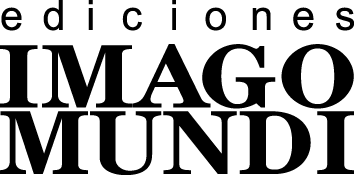
\includegraphics[width=20mm]{./media/logo-imago-ByW.png}
\end{figure}

% página 6
\newpage
\thispagestyle{empty}
\begin{figure}[t]
\centering
\vspace{-10mm}

\includegraphics[width=20mm]{./media/desconocido.png}\\
\end{figure}

\noindent Gala Aznarez Carini; Emmanuel Biset; Andrés Daín et al. \\
\noindent Ontologías Políticas. 1a ed. Buenos Aires: 2023.\\
\noindent \ztotpages\ p.; \valorEspecifico. ISBN 978-950-793-000-0 \\
\noindent 1. \\
\noindent CDD .\\
\noindent Fecha de catalogación: 28/06/2025 \\
\noindent \textcopyright~2025, Villalba, Javier A. \\
\noindent \textcopyright~2025, Ediciones Imago Mundi\\
\noindent Imagen de tapa: Marta M.\\
\noindent Hecho el depósito que marca la ley 11.723\\
\noindent Impreso en Argentina, tirada de esta edición: 1000 ejemplares\\

\vfill

\noindent \qrcode[height=2cm]{https://www.edicionesimagomundi.com/}\bigskip

\noindent Ninguna parte de esta publicación, incluido el diseño de cubierta, puede ser reproducida, almacenada o transmitida de manera alguna ni por ningún medio, ya sea eléctrico, químico, mecánico, óptico, de grabación o de fotocopia, sin permiso previo por escrito del editor. Este libro se terminó de imprimir en el mes de xxxx de 20xx en San Carlos Impresiones, Virrey Liniers 2203, Ciudad Autónoma de Buenos Aires, República Argentina.

\Author{Sumario}
\tableofcontents
	\else
	\ifBNPDF
	\ifPDF
\PaginaEnBlanco
\PaginaEnBlanco
	\else
	\ifBNPDF
	\PaginaEnBlanco
	\PaginaEnBlanco
	\fi
\fi

% página 3
\newpage
\thispagestyle{empty}
{\textcolor{white}{.}}

\vspace{30mm}

\begin{center}
	\LARGE{Ontologías Políticas}
\end{center}

% página 4
\newpage
\thispagestyle{empty}
{\textcolor{white}{.}}

% página 5
\newpage
\thispagestyle{empty}

\vspace{30mm}

\begin{center}
	\LARGE{Ontologías Políticas}\\\vspace{10mm}

	\Large{}
\end{center}

\vspace{10mm}

\begin{center}%,draft
{\sc\large{Gala Aznarez Carini\\
		Emmanuel Biset\\
		Andrés Daín\\
		Roque Farrán\\
		Daniel Groisman\\
		Manuel Moyano\\
		Juan Manuel Reynares\\
		Aurora Romero\\
		Mercedes Vargas}}\\ %compiladoras
\end{center}



\vfill

\begin{figure}[b]
\centering
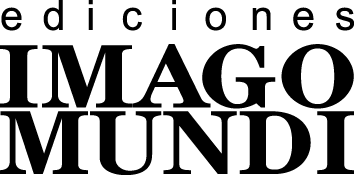
\includegraphics[width=20mm]{./media/logo-imago-ByW.png}
\end{figure}

% página 6
\newpage
\thispagestyle{empty}
\begin{figure}[t]
\centering
\vspace{-10mm}

\includegraphics[width=20mm]{./media/desconocido.png}\\
\end{figure}

\noindent Gala Aznarez Carini; Emmanuel Biset; Andrés Daín et al. \\
\noindent Ontologías Políticas. 1a ed. Buenos Aires: 2023.\\
\noindent \ztotpages\ p.; \valorEspecifico. ISBN 978-950-793-000-0 \\
\noindent 1. \\
\noindent CDD .\\
\noindent Fecha de catalogación: 28/06/2025 \\
\noindent \textcopyright~2025, Villalba, Javier A. \\
\noindent \textcopyright~2025, Ediciones Imago Mundi\\
\noindent Imagen de tapa: Marta M.\\
\noindent Hecho el depósito que marca la ley 11.723\\
\noindent Impreso en Argentina, tirada de esta edición: 1000 ejemplares\\

\vfill

\noindent \qrcode[height=2cm]{https://www.edicionesimagomundi.com/}\bigskip

\noindent Ninguna parte de esta publicación, incluido el diseño de cubierta, puede ser reproducida, almacenada o transmitida de manera alguna ni por ningún medio, ya sea eléctrico, químico, mecánico, óptico, de grabación o de fotocopia, sin permiso previo por escrito del editor. Este libro se terminó de imprimir en el mes de xxxx de 20xx en San Carlos Impresiones, Virrey Liniers 2203, Ciudad Autónoma de Buenos Aires, República Argentina.

	\Author{Sumario}
	\tableofcontents
		\else
		\ifPNGEPUB
		\ifPDF
\PaginaEnBlanco
\PaginaEnBlanco
	\else
	\ifBNPDF
	\PaginaEnBlanco
	\PaginaEnBlanco
	\fi
\fi

% página 3
\newpage
\thispagestyle{empty}
{\textcolor{white}{.}}

\vspace{30mm}

\begin{center}
	\LARGE{Ontologías Políticas}
\end{center}

% página 4
\newpage
\thispagestyle{empty}
{\textcolor{white}{.}}

% página 5
\newpage
\thispagestyle{empty}

\vspace{30mm}

\begin{center}
	\LARGE{Ontologías Políticas}\\\vspace{10mm}

	\Large{}
\end{center}

\vspace{10mm}

\begin{center}%,draft
{\sc\large{Gala Aznarez Carini\\
		Emmanuel Biset\\
		Andrés Daín\\
		Roque Farrán\\
		Daniel Groisman\\
		Manuel Moyano\\
		Juan Manuel Reynares\\
		Aurora Romero\\
		Mercedes Vargas}}\\ %compiladoras
\end{center}



\vfill

\begin{figure}[b]
\centering
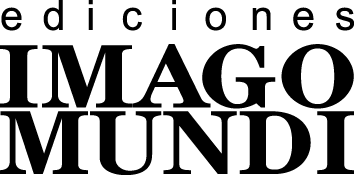
\includegraphics[width=20mm]{./media/logo-imago-ByW.png}
\end{figure}

% página 6
\newpage
\thispagestyle{empty}
\begin{figure}[t]
\centering
\vspace{-10mm}

\includegraphics[width=20mm]{./media/desconocido.png}\\
\end{figure}

\noindent Gala Aznarez Carini; Emmanuel Biset; Andrés Daín et al. \\
\noindent Ontologías Políticas. 1a ed. Buenos Aires: 2023.\\
\noindent \ztotpages\ p.; \valorEspecifico. ISBN 978-950-793-000-0 \\
\noindent 1. \\
\noindent CDD .\\
\noindent Fecha de catalogación: 28/06/2025 \\
\noindent \textcopyright~2025, Villalba, Javier A. \\
\noindent \textcopyright~2025, Ediciones Imago Mundi\\
\noindent Imagen de tapa: Marta M.\\
\noindent Hecho el depósito que marca la ley 11.723\\
\noindent Impreso en Argentina, tirada de esta edición: 1000 ejemplares\\

\vfill

\noindent \qrcode[height=2cm]{https://www.edicionesimagomundi.com/}\bigskip

\noindent Ninguna parte de esta publicación, incluido el diseño de cubierta, puede ser reproducida, almacenada o transmitida de manera alguna ni por ningún medio, ya sea eléctrico, químico, mecánico, óptico, de grabación o de fotocopia, sin permiso previo por escrito del editor. Este libro se terminó de imprimir en el mes de xxxx de 20xx en San Carlos Impresiones, Virrey Liniers 2203, Ciudad Autónoma de Buenos Aires, República Argentina.

		\Author{Sumario}
		\tableofcontents
		\fi
	\fi
\fi

\ifHTMLEPUB
\tableofcontents
\fi

\chapter{Presentación}
\Author{ } % Esta línea es necesaria
\chaptermark{ }
\sectionmark{ } % Para evitar que "Sumario" siga apareciendo

Si muchas veces el trabajo intelectual parece darse en soledad, en el caso de este libro se trata de un pensar conjunto. A lo largo del tiempo hemos puesto en común nuestros trabajos individuales, los hemos sometido a discusión, hemos discrepado, compartido lecturas, y así, hemos tratado de escucharnos. De modo que este texto surge de un ejercicio colectivo de pensamiento nucleado en torno al \enquote{Programa de Estudios en Teoría Política} radicado en el \gls{@glo232-ciecs} de la \gls{@glo235-unc} y el \gls{@glo233-conicet}.

Desde el pensar en común han surgido escritos singulares, diversos, plurales, que en su vacilación y fortaleza decidimos publicar para seguir dándole vueltas a preguntas, problemas, inquietudes, malestares y alegrías que nos convocan. La singularidad de cada texto no debe de dejar notar que los mismos están atravesados, de un lado, por una reflexión teórico-política y, de otro lado, por el trabajo desde autores que constituyen una constelación heredera de ciertas transformaciones surgidas del pensamiento francés de la década del `60. Autores como Althusser, Derrida, Foucault, Lacan, Rancière, Agamben, Nancy o Badiou han sido convocados. Cada texto, entonces, en la tensión entre singularidad y comunidad.

Publicamos para seguir la conversación infinita en la que estamos.

\chapter{¿Por qué ontologías políticas?}
\Author{ } % Esta línea es necesaria
\chaptermark{Introducción}
\sectionmark{ } % Para evitar que "Sumario" siga apareciendo

1.

La apuesta colectiva de este libro surge de un posicionamiento frente a los estudios contemporáneos sobre la política. Con la expresión \enquote{ontología política} planteamos un distanciamiento respecto al privilegio del abordaje gnoseológico, puesto que la teoría política, la filosofía política o el pensamiento impolítico suponen un vínculo singular entre el saber y la política. Tratándose siempre de las posibilidades o imposibilidades abiertas por esa vinculación entre un área del saber y determinadas formas políticas. Esto ha llevado a cuestionamientos recurrentes en el pensamiento contemporáneo a la filosofía o teoría política en tanto las mismas determinaciones de lo filosófico o lo teórico imposibilitarían abordar en toda su complejidad la política sin llevar a su subordinación o eliminación.

Frente a ello, creemos oportuno hablar de ontologías políticas en tanto se trata de formas de pensar la configuración del mundo y no sólo elaboraciones teóricas. Esto se debe a que en tal caso se parte, al mismo tiempo, de cierta definición de lo teórico y de un área de la realidad nombrada con el término política. Las diversas ontologías políticas presentadas aquí no surgen de una relación exterior entre conocimiento y realidad, o entre sujeto y objeto, sino que son formas de pensar cómo se constituye el mundo como tal. De un lado, se destituye el privilegio de la teoría en cuanto no se define una forma de conocer, sino una forma de constituir el mundo. De otro lado, la política ya no se considera un área determinada dentro de la realidad, sino el mismo proceso de constitución de lo real (lo que supone un juego infinito entre lo constituyente y lo constituido).

Pretendemos poner en primer plano la cuestión del ser, su interrogación, rompiendo con la sutura epistemológica que sostiene que las teorías sólo pueden preguntarse por las condiciones de posibilidad del conocimiento. De modo que la primera aproximación a un posicionamiento ontológico para abordar la política surge del distanciamiento y la subversión de las perspectivas epistemológicas, puesto que no se trata del conocimiento exterior de un objeto determinado, sino del pensamiento del \emph{\gls{@glo234-serquaser}}, es decir, de las maneras en las que se configura de uno u otro modo.

La apuesta entonces es pasar del conocer al ser.

2.

La palabra ontología tal como lo indica su etimología nombra el \enquote{discurso sobre el ser}, es decir, la relación entre el discurso, el lenguaje o la razón con el ser en tanto que ser. Resulta central señalar que no nos referimos al ser en tanto que ser \rdm{el ser en sí mismo} sino al o los \emph{discursos} sobre el ser. La cuestión es pensar de qué modo, entonces, se da el vínculo entre discurso y ser tal como lo pensamos aquí.

Desde lo establecido en el apartado anterior es posible señalar que nos diferenciamos de dos perspectivas al respecto. En primer lugar, nos diferenciamos de una perspectiva que identifica pensamiento y ser, esto es, que parte de la \enquote{identidad} entre ambos. En segundo lugar, nos separamos de aquellas posiciones que la piensan como una relación de exterioridad, esto es, un discurso que se dirige al mundo (en su forma moderna implicaría el esquema de la representación donde el sujeto fundamenta la legitimidad del objeto). Para no pensar en términos de identidad o exterioridad, partimos de la copertenencia entre ser y pensar. Esta implicancia mutua da cuenta de una vinculación necesaria (de ahí la ausencia de identidad) pero sin pensarla como dos dimensiones opuestas (de ahí la ausencia de exterioridad).

El discurso sobre el ser no es un discurso sobre una dimensión u objeto externo, sino un discurso que en la pregunta por el ser abre su misma posibilidad. Dicho en otros términos, la identificación es imposible en tanto existe un distanciamiento propio de la pregunta que abre, pero es el mismo ser quien realiza la pregunta, en tanto no existe un algo más allá del ser que pregunte por el ser. Al preguntar por el ser en tanto que tal surge un pliegue en el mismo ser. Por ello ser y pensar son lo mismo sin ser idénticos.

La forma de los discursos sobre el ser que aquí presentamos es la pregunta o el preguntar. O mejor, los discursos presentados están sobredeterminados por la forma-pregunta. La pregunta por el ser es lo que \emph{abre} el mismo ser: no lo crea, no lo reconoce, no lo experimenta, no lo percibe, sino que es una indagación o una cuestión que abre una grieta en lo existente al preguntar por su modo de ser. En este sentido, la pregunta se dirige de un modo singular a la multiplicidad de lo existente en tanto indaga en esa diversidad por sus maneras de ser.

Los discursos sobre el ser en tanto que apertura (grieta, hiancia, brecha) de lo dado suponen dos cosas. Por un lado, que lo dado al mismo tiempo que es lo único existente no es sólo lo dado. Existe una diferencia inherente en cuanto la pregunta permite diferenciar entre lo dado y aquello que lo hace ser como tal. Esto es lo que, siguiendo a Heidegger, podemos llamar diferencia ontológica\index[concepto]{Diferencia!ontológica}. La pregunta es así la condición de posibilidad incesantemente renovada de la diferencia entre lo dado como existente y su modo de ser específico. Por otro lado, al introducir una grieta en lo real, lo dado deja de ser evidencia o inmediatez, para convertirse en algo cuya constitución es contingente. La pregunta ontológica abre al ser como pura posibilidad. Esto nos permite señalar que una indagación ontológica es aquella que piensa los modos en que se configura lo dado, o mejor, los procesos contingentes desde los que se estabiliza una forma de lo existente. Lo posible no es algo más allá del mundo, sino su misma condición, y por lo tanto la posibilidad de ya no ser como tal.

Por todo esto, los discursos sobre el ser \rdm{las ontologías propuestas aquí} tiene un estatuto cuasi-trascendental. \emph{Trascendental} en tanto abren lo dado más allá de lo dado sin conducir a otro existente. Desde la tradición kantiana lo trascendental indica un estatuto singular: la condición de posibilidad. \emph{Cuasi} en tanto la pregunta supone condiciones de posibilidad y de imposibilidad y, al mismo tiempo, no existe un trascendental puro sino que siempre se encuentra contaminado de facticidad o empiricidad.

Esta última indicación nos permite afirmar que nuestros discursos están producidos de manera situada y por ello se ubican en la tensión entre las discusiones teóricas y los acontecimientos políticos. La situacionalidad no la entendemos como la ubicación en determinado contexto histórico, que otra vez podríamos reconstruir como sujetos cognoscentes, sino como la contaminación irreductible de cualquier pureza teórica con lo que acontece. Esto no significa sólo atenerse a lo existente, sino indagando sus condiciones abrir hacia un más allá incierto,la incertidumbre no es coyuntural sino su mismo exceso.

Los discursos sobre el ser son el preguntar que abre lo dado más allá de lo dado: a su modo contingente de configuración. Esto implica pasar de la pregunta por el \enquote{qué} a la pregunta por el \enquote{cómo}. Se trata de pensar el cómo de la multiplicidad de lo dado sin remitir a algo más allá de ello. Se acentúa así el proceso de constitución de lo existente, lo que nos permite señalar que las condiciones de posibilidad son condiciones de existencia.

3.

El término ontología tal como lo comprendemos aquí supone una determinada concepción de lo dado que se opone a dos perspectivas o, en otros términos, la singularidad de nuestra propuesta se comprende en el distanciamiento respecto del \gls{@glo236-esencialismo} y del \gls{@glo237-constructivismo}. Primero, al acentuar la dimensión ontológica como apertura en tanto posibilidad nos oponemos a cualquier posición metafísica que fije lo existente, fundándolo de modo trascendente o inmanente. Esto significa que aquello que existe no tiene una esencia o idea que pueda ser fijada de un modo definitivo, por lo que existe una inestabilidad constitutiva donde se producen estabilizaciones precarias. Segundo, nos distanciamos de cierto constructivismo que desde metáforas arquitectónicas supone un agente, una forma o idea y una materia informe. Este constructivismo parte de que lo dado es construido desde una alteridad respecto de lo dado, sea un sujeto individual, sea la sociedad en su conjunto, sea dios. Lo que, al mismo tiempo que cuestiona el esencialismo, restituye un lugar trascendente respecto del mundo que posibilita su construcción (constructivismo sobredeterminado por una especie de voluntarismo que bajo las formas del lenguaje, la cultura, el sujeto, la racionalidad o la sociedad ubican lo posible en un exterior, es decir, la contingencia como algo exterior a lo existente).

El doble distanciamiento, respecto del esencialismo y del constructivismo, permite comprender el vínculo entre ontología e historia que plantamos aquí. Si desde el esencialismo se afirma la perennidad de una idea o concepto, el constructivismo lo cuestiona señalando que existe una historicidad contextual constitutiva de los lenguajes y las instituciones políticas. Ahora bien, el problema del constructivismo es que la historicidad se ubica en un contexto exterior a aquello que historiza. Un concepto varía, así, porque es ubicado en uno u otro momento histórico. Frente a ello, aquí postulamos un historicismo radical, lo que significa dos cosas: por una parte, que la historicidad no es exterior o contextual sino inherente a un lenguaje o institución; por otra parte, que la indagación ontológica es historial y no histórica, se trata de la diferencia que hace posible la historia misma.

Desde nuestra perspectiva, lo dado al mismo tiempo es y no es lo único existente. Esta paradoja se entiende si afirmamos que no existe algo más allá, un fundamento exterior que dé origen a lo dado (cuya figura histórica por excelencia ha sido la del dios creador), pero al mismo tiempo la pregunta abre lo existente más allá de su existencia: abre una grieta en cuanto se establece la diferencia entre lo existente y su modo de ser (o entre ente y ser para retomar los términos heideggerianos).

Las ontologías como formas de indagación por el cómo de lo dado destituyen la explicación causal que supone una relación exterior entre el efecto y su causa, que también conlleva una temporalidad lineal donde existe una precedencia de la causa sobre el efecto. Aquí partimos de lo dado para indagar cómo determinada configuración lo ha constituido como tal, por lo que nunca se cierra como algo autoconstituido. Debido a que el ente nunca se constituye a sí mismo (imposibilidad de cierre), eso le imprime un carácter ontológico a la indagación, de su inacabamiento a la apertura constitutiva.

Por estos motivos, más allá del esencialismo y del constructivismo, partimos de la ontología como indagación sobre la \emph{constitución} de lo dado.

4.

La utilización del calificativo \enquote{políticas} para referirnos a las ontologías presentadas busca mantenerse en la indeterminación. Partimos no sólo de la variación histórica del concepto de política, sino de su contingencia, lo que significa que aun cuando fuera posible sistematizar la totalidad de las definiciones dadas de política no sería posible fijar su sentido. Esto nos permite afirmar que no existe concepto o esencia de la política. O, en otros términos, que la política es constitutivamente inadecuada a su concepto. Por lo que el concepto mismo se configura en su imposibilidad de cierre e inacabamiento significativo (esto no quiere decir que no se afirme a través de nuevos términos significantes)

La política es aporética, es decir, al mismo tiempo que está saturada por múltiples definiciones existe una falta que imposibilita esa saturación. Lo aporético se da en el cruce entre exceso y falta que se juega en distintos niveles discursivos y términos electivos (entre ontología y política, lo político y la política, la teoría y la praxis, etc.). Siendo así, la política comienza siempre con una lucha por la definición de la política, por la estabilización precaria de los límites que permiten considerar a algo político. Por esto mismo, la sobredeterminación de una definición de política desde el conflicto, el orden, el acuerdo, la tragedia, es secundaria respecto a su radical inestabilidad. Así, como no existe un núcleo último al cual acceder, sólo es posible moverse en una u otra sobredeterminación.

La inestabilidad también se ubica en la política como dispositivo: la precaria fijación de un sentido de política surge en la tensión entre las formas-políticas y las formas-veritativas de una época. Con el término forma-política nos referimos a las instituciones, prácticas, relaciones políticas de una determinada época. Con el término forma-veritativa nos referimos al modo como se configura el saber y la verdad también epocalmente. La política, así, es la tensión entre formas políticas y veritativas en cuanto nunca se corresponden de modo pleno.

Con esto queremos indicar, primero, que no partimos de una definición dada de política, sino que la misma surge en los diferentes textos (apostando así por la indefinición o la definición en acto en cada apuesta de pensamiento); segundo, que la política no tiene un vínculo privilegiado con la ontología, no existe una relación necesaria entre una y la otra, sino que aquí pensamos ontologías que en su pluralidad pueden ser calificadas de políticas. Puede haber otras ontologías (estéticas, matemáticas, etc.) y puede haber otras ontologías políticas. Aquí presentamos distintos discursos que no tratan la política como un área determinada, sino como formas posibles que puede adquirir la configuración del mundo.

5.

Atender a la constitución de lo dado es indagar por su modo de ser. Esta indagación, señalábamos, no parte simplemente de la multiplicidad o pluralidad de lo existente, sino que abre hacia su dimensión ontológica. Esto conlleva un doble movimiento: un momento negativo puesto que al indagar por el modo de ser se niega lo existente como tal, el ser de algo no es lo dado, no es lo ente, y así es la nada de lo ente; pero también un momento positivo en tanto allí aparecen los modos de constitución de lo existente como procesos de configuración.

Una perspectiva ontológica como la propuesta aquí de ningún modo legitima el mundo como tal, puesto que parte de su socavamiento. Se trata de una indagación que abre lo existente a su configuración desde un trasfondo de posibilidades. De ahí que rompa con la lógica de la legitimidad que supone la exterioridad del juicio. En otros términos, la apuesta por pensar ontologías políticas supone una redefinición de lo que se entiende por tarea crítica del pensamiento. La pregunta por la legitimidad de lo dado, desde su dependencia del dispositivo político moderno, se dirige a preguntar por el porqué de lo existente. Esto es, supone la estructura del juicio en tanto el tribunal de la razón juzga lo existente desde un criterio y conlleva por ello mismo la fijación de un fundamento que otorgue o niega la legitimación (en términos históricos sería posible mostrar el paso de una fundamentación trascendente a una inmanente).

La ontología como crítica más allá de la crítica no juzga lo real desde la razón, sino que abre lo real a su posibilidad. Por ello mismo se trata de una posición que constituye en sí misma una apuesta política. No se trata de no aceptar lo dado en cuanto no se ajusta a un criterio previamente establecido, sino de mostrar que lo dado no es tal, que su modo de ser es la misma posibilidad.

Nuestra apuesta teórica, nuestra apuesta política: preguntar para abrir lo posible \emph{en} lo dado.

\emph{Gala Aznarez Carini, Emmanuel Biset, Andrés Daín, Roque Farrán, Daniel Groisman, Manuel Moyano, Juan Manuel Reynares, Aurora Romero, Mercedes Vargas.}

\mainmatter

\chapter[\textbf{Emmanuel Biset}\\ Ontología de la diferencia]{Ontología de la diferencia}
\Author{Emmanuel Biset}
\chaptermark{Ontología de la diferencia}
\nombreautor{Emmanuel Biset}

\epigraph{\emph{\enquote{La diferencia entre Deleuze y Derrida como diferencia propia \rdm{y en consecuencia, como identidad en sí dividida} de un tiempo, de un presente de pensamiento que habrá formado una inflexión decisiva, sigue estando por pensar}.}}{Jean-Luc Nancy}

\section{Introducción}

Existen ciertos conceptos y no otros que marcan determinada época. Conceptos que al mismo tiempo que constituyen un índice del tiempo vivido intervienen en él. Uno de esos conceptos es el de \enquote{diferencia}, concepto que se ha constituido como un indicio central para pensar el mundo contemporáneo en, por lo menos, dos sentidos. De un lado, el término diferencia ha servido para designar toda una corriente del pensamiento contemporáneo: aquello que se ha denominado \enquote{filosofía de la diferencia}. De otro lado, el término diferencia en un sentido político viene a designar una época en la cual se han pluralizado las formas de vida y la alteridad se ha convertido en un problema ineludible. Un pensamiento de la diferencia en política parece remitir a la pluralidad expandida del mundo contemporáneo y así a las discusiones sobre multiculturalismo, interculturalidad, etc., y al problema de la alteridad radical, y así a las discusiones sobre migrantes, sexualidades, pueblos originarios, etc.

Aquí no se indaga la supuesta pluralidad contemporánea, sino en la discusión de diferentes pensamientos de la diferencia se da cuenta del estatuto ontológico de la diferencia. Cuando nos referimos a estatuto ontológico de la diferencia señalamos que no se trata de pensar la diferencia entre elementos de una realidad ya constituida, sino de la diferencia como constituyente\index[concepto]{Diferencia!como constituyente} de esa misma realidad. Este mismo problema surge en el plano de la significación. Si queremos precisar el significado de un término como \enquote{diferencia} lo reducimos al plano de un signo entre otros, siendo que la diferencia menta el mismo proceso de significación. Por lo que el primer objetivo del texto es mostrar cómo se ha roto con aquellos planteos que hacen de la diferencia algo secundario respecto a elementos constituidos. Para cumplir este objetivo se avanza en tres pasos.

En un primer momento se muestra el contexto en el cual la diferencia dejó de ser un concepto entre otros para caracterizar a toda una generación de autores. De este contexto destacamos el enfrentamiento con la dialéctica hegeliana, la elaboración de una filosofía de la diferencia en Heidegger y el lugar de la diferencia lingüística en el estructuralismo. Planteos que no sólo se muestran como indicios de época, sino que articulan una serie de supuestos desde los que se elabora el pensamiento de la diferencia.

En un segundo momento, se analiza la diferencia en los pensamientos de Gilles Deleuze y Jacques Derrida. Si estos autores son identificados como los autores de la diferencia, el objetivo del texto es indicar qué sentido adquiere la diferencia en cada uno, no sólo mostrando sus antecedentes, sino aquellos aspectos que los distancian. Será la referencia a Hegel aquello que permita notar dos filosofías de la diferencia.

En un tercer momento, se muestra el carácter político de una ontología de la diferencia.\footcite[\emph{Ontología diferencial} es el título de una propuesta reciente de Miguel de Beistegui que cruza los planteos de Heidegger y Deleuze para elaborar una filosofía que escape a su fragmentación. Aquí, a diferencia de Beistegui, se trata de pensar desde una perspectiva política esta ontología diferencial. Véase][]{@6960-BEISTEGUI2004} Para ello, se dan argumentos en dos sentidos: se analiza el carácter \enquote{constituyente} de la diferencia a partir de la distinción entre lo óntico, lo ontológico y lo trascendental, y se propone, a distancia de ciertos planteos contemporáneos, la politicidad de la diferencia como procesos de temporalización y espaciamiento en tanto condiciones de existencia de lo dado. Este apartado, indicativo ante todo, pretende ser el aporte del texto.

En resumidas cuentas, efectuamos un recorrido singular para mostrar el carácter político de la diferencia. Lo cual nos permite dar cuenta de una particular vinculación teórica entre ontología y política.

\section{Dialéctica y diferencia}

Al comenzar \emph{Diferencia y repetición}, Gilles Deleuze escribe sobre el contexto en que surge el problema de la diferencia:

\begin{quote}
El tema aquí tratado se encuentra, sin duda alguna, en la atmósfera de nuestro tiempo. Sus signos pueden ser detectados: la orientación cada vez más acentuada de Heidegger hacia una filosofía de la Diferencia ontológica; el ejercicio del estructuralismo, basado en una distribución de caracteres diferenciales en un espacio de coexistencia; el arte de la novela contemporánea, que gira en torno de la diferencia y de la repetición, no sólo en su reflexión más abstracta sino también en sus técnicas efectivas; el descubrimiento, en toda clase de campos, de un poder propio de repetición, que sería tanto la del inconsciente como la del lenguaje y del arte. Todos estos signos pueden ser atribuidos a un anti-hegelianismo generalizado: la diferencia y la repetición ocuparon el lugar de lo idéntico y de lo negativo, de la identidad y de la contradicción.\footcite[15]{@6961-DELEUZE2002}
\end{quote}

Desde la perspectiva de Deleuze, el pensamiento de la diferencia puede ser entendido desde un antihegelianismo generalizado, es decir, se comprende como reacción ante la hegemonía de la dialéctica. Si bien es posible indicar que existen otras corrientes con una presencia ineludible \rdm{así la fenomenología}, la noción de diferencia surge en oposición a cierta interpretación de Hegel. Esto resulta central, pues en gran medida la historia intelectual del pensamiento francés contemporáneo comienza con la lectura que realiza Alexander Kojève de la fenomenología hegeliana

\begin{quote}
Si existe un signo del cambio de mentalidades \rdm{rebelión contra el neo-kantismo, eclipse del bergsonismo}, desde luego que es la vuelta firme de Hegel. Éste, proscrito por los neokantianos, de repente se vuelve, curiosamente, un autor de vanguardia citado con respeto en los círculos más avanzados. Este renacimiento parece deberse a dos razones principales. Una es el nuevo período de interés hacia el marxismo, tras la revolución rusa.(\dots) La otra razón es la influencia del curso pronunciado por Alexandre Kojève en la Escuela Práctica de Altos Estudios a partir de 1933 y que se prolongará hasta 1939. \footcite[28]{@6962-DESCOMBES1998}
\end{quote}

La relación con Kojève es central porque permite entender cómo se lee a Hegel en el pensamiento francés contemporáneo. Una interpretación en la cual se recupera la \emph{Fenomenología del espíritu}, apartándose de las lecturas que ven en el filósofo alemán sólo la hipóstasis de la razón. Esta lectura acentúa el origen irrazonable de lo razonable en relación con las filosofías de la existencia de principios de siglo, es decir, en proximidad con Husserl y Heidegger. Ante las lecturas panlogistas que destacan la identificación de lo real y lo racional, en el Hegel de Kojève el pensamiento es el movimiento de la razón hacia su otro, y por ello es una ampliación de la razón. Se trata de la \emph{negatividad} pensada en términos antropológicos, o mejor, de una antropología ontológica donde el hombre es el motor de la historia: \enquote{\ldots antropológico en el sentido que se trata ahí de \enquote{existencia}, es decir, de deseo y de \emph{acción}. Hegel no es simplemente un intelectualista: sin la creación por la acción negadora no hay contemplación de lo dado}.\footcite[53]{@6963-KOJEVE1996} En esta perspectiva, la dialéctica expresa un humanismo, esto es, la dialéctica es ontológicamente humanista porque todo lo que tiene sentido se decide en la historia humana entendida como acción transformadora del hombre.

La lectura de Kojève será central al trabajar Hegel a la luz de la filosofía contemporánea, marcando así a toda una generación del pensamiento francés entre quienes se puede citar a Georges Bataille, Raymond Aron, Alexandre Koyré, Pierre Klossowski, Jacques Lacan, Maurice Merleau-Ponty, Eric Weil. La dialéctica goza de un importante prestigio en la Francia posterior a 1930. Quizá el mayor indicio de esta relevancia se encuentra en \emph{La crítica de la razón dialéctica} de Jean Paul Sartre, publicada en 1960, y donde el marxismo como razón dialéctica constituye el \enquote{horizonte irrebasable} de nuestro tiempo: \enquote{Nuestro tiempo será, pues, \emph{crítico} porque tratará de determinar la validez y los límites de la Razón dialéctica, lo que supone indicar las oposiciones y los lazos de esta Razón con la Razón analítica y positivista}. \footcite[11]{@6964-SARTRE1995}

Frente a esta generación, ciertos autores que comienzan a escribir en las décadas del 50 y 60 se definen por su crítica a la dialéctica. Si bien existen diferencias de estilo, de acento, de interpretación, se comparte esta oposición al hegelianismo. Autores como Michel Foucault, Gilles Deleuze, Jacques Derrida, se caracterizan por la ruptura con Hegel. Señala Michel Foucault: \enquote{(\dots) toda nuestra época, bien sea por la lógica o por la epistemología, bien sea por Marx o por Nietzsche, intenta escapar de Hegel}. \footcite[59]{@6984-FOUCAULT1973} Esta ruptura con Hegel resulta central para pensar el contexto de emergencia del pensamiento de la diferencia. Pues vale recordar que la dialéctica hegeliana se construye como una lógica donde la alteridad tiene un lugar constitutivo. La negatividad nombra un movimiento de alienación, de un hacerse otro. La diferencia como \emph{mediación} es constitutiva del movimiento dialéctico. Al mismo tiempo, la identidad juega un rol central, pues la mediación se produce en vistas a una reconciliación final. En este marco es necesario destacar que la crítica a Hegel surge de la oposición entre identidad y diferencia, pues la cuestión es de qué modo la predominancia de la identidad reduciría la diferencia, es decir, la alteridad a la mismidad. Desde esta perspectiva, la dialéctica al considerar la diferencia como negación produciría un sometimiento de lo otro en una articulación superior, en una unidad idéntica superior jerárquicamente.

En este contexto de crítica a la dialéctica es posible ubicar dos de los indicios de época que Deleuze señala en su cita: la filosofía de la diferencia de Martin Heidegger y el estructuralismo de Ferdinand de Saussure. En Heidegger aparece explícitamente la confrontación entre dialéctica y diferencia en un escrito central para la época: \emph{Identidad y diferencia}. Publicado en el año 1957, el texto se compone de dos conferencias: \enquote{El principio de identidad} y \enquote{La constitución onto-teo-lógica de la metafísica}. Si la diferencia ontológica es constitutiva del pensamiento heideggeriano, es su radicalización en una filosofía de la diferencia aquello que constituye un indicio central para el pensamiento francés de la década del 60. En el segundo de los artículos citados, texto de 1957 escrito como finalización de un curso sobre Hegel, Heidegger nomina su pensamiento desde la noción de diferencia oponiéndola a la dialéctica hegeliana:

\begin{quote}
Para Hegel, el asunto del pensar es el ser en relación con lo que fue pensado sobre lo ente en el pensar absoluto y en cuanto tal. Para nosotros, el asunto del pensar es lo mismo, y por lo tanto, el ser, pero el ser desde la perspectiva de su diferencia con lo ente. Digámoslo con más precisión todavía: para Hegel, el asunto del pensar es el pensamiento como concepto absoluto. Para nosotros, el asunto del pensar \rdm{usando un nombre provisional}, es la diferencia \emph{en cuanto} diferencia. \footcite[107]{@6965-HEIDEGGER1988}
\end{quote}

La noción de diferencia retomando la diferencia ontológica sirve aquí para nombrar la distancia con Hegel. De modo que en Heidegger encontramos claramente la oposición entre pensamiento de la diferencia y filosofía dialéctica. Si esta oposición constituye el primer aspecto a destacar contextualmente, el segundo aspecto es la necesidad de pensar la diferencia en cuanto diferencia. Esto significa: pensar la diferencia en cuanto tal\index[concepto]{Diferencia!en cuanto tal}. Este \enquote{en cuanto tal} permite notar dos cosas respecto al tratamiento de la diferencia: primero, que con el término diferencia no se nombra la diferencia de cosas existentes en el mundo: la diferencia óntica\index[concepto]{Diferencia!óntica}; segundo, que tampoco el término diferencia se dirige a una distinción establecida por el entendimiento. Heidegger nos ayuda a comprender que con este término no se está aludiendo a dos cosas distintas en el mundo ni a una distinción establecida por el entendimiento humano. Estas distinciones son secundarias puesto que suponen, ante todo, la identidad de aquellas cosas que luego entrarán en una relación diferencial. En cualquiera de estos casos la diferencia es sobreañadida a una realidad preexistente, sea como representación del entendimiento, sea como vinculación en la experiencia. Por lo que la diferencia se reduce a una diferencia entre entes.

Heidegger señala que la cuestión es pensar la diferencia entre ente y ser. Esta diferencia no es posterior a dos realidades llamadas por caso ser y ente, sino que ser y ente aparecen a partir de la diferencia. Esto resulta central, pues la diferencia no es posterior, sino es la misma \emph{posibilidad} del ser y el ente, por lo que existe una \enquote{primacía ontológica} de la diferencia sobre el ser y el ente. No se puede distinguir ser y ente como dos entes singulares, pues en tal caso se elimina la pregunta por la diferencia ontológica. Se trata de pensar en el ente mismo el ser, por lo que ser y ente no son algo distinto, son lo mismo, o mejor, es la diferencia en lo mismo: \enquote{Ser y ente son lo Mismo; sólo en la diferenciación entre ser y ente está unido de propio lo Mismo (el ser del ente, el ente en su ser) en la unidad con él mismo. Ser no es algo distinto de lo ente; si fuera algo distinto sería, una vez más, ente, y la Diferencia ontológica quedaría invertida en mera Diferencia óntica}. \footcites[176]{@6966-POGGELER1993}[Si ya tempranamente la cuestión de la diferencia ontológica resulta central, será su radicalización como pensamiento de la diferencia aquello que constituya un marco de referencia para la filosofía francesa. Radicalización en cuanto se trata de pensar la diferencia en cuanto diferencia. Pensamiento de la diferencia en cuanto tal que se enfrenta a una dificultad constitutiva debido a que existen diversos términos en alemán que el autor utiliza para nombrarla. Véase][]{@6990-RESTA1988} Esta será la principal crítica a la tradición, convertir al ser en un ente más, incluso un ente supremo que fundaría el resto de los entes (onto-teo-logía). Pero si el ser se piensa como un ente entre otros, olvidamos la pregunta por la diferencia ontológica. De modo que el pensamiento de Heidegger resulta central porque, de un lado, aparece una \enquote{filosofía de la diferencia} en expresa confrontación con Hegel y, de otro lado, un pensamiento de la diferencia en cuanto tal \index[concepto]{Diferencia!en cuanto tal} lleva a la formulación de la diferencia ontológica, es decir, a mostrar el estatuto ontológico de la diferencia. En otros términos, la diferencia no es posterior a la existencia de cosas en el mundo, sino que es aquello que hace posible al mundo como tal.

El otro indicio ineludible del contexto es el estructuralismo. \footcite[Francois Dosse en su historia intelectual del estructuralismo señala la relevancia para la década del 60 del cruce entre el programa nietzscheano-heideggeriano y el estructuralismo: \enquote{La búsqueda heideggeriana del logos se une aquí con la genealogía nietzscheana, y ambas encontraron en el estructuralismo un magnifico destino. La crítica del etnocentrismo, del eurocentrismo, van a acentuarse en los años cincuenta y sesenta con la marea estructuralista, que va a retomar el paradigma crítico del nietzscheao-heideggerismo}][416]{@6967-DOSSE2004} No se trata de una teoría entre otras, sino del marco teórico que hegemoniza la época. Una \enquote{aventura de la mirada} que pretende atravesar diversos campos proponiendo una forma singular de indagar todo objeto. En el estructuralismo la noción de diferencia no es una más, sino que puede considerarse su núcleo duro. Como es sabido, Saussure inaugura la ciencia del lenguaje en cuanto define la naturaleza del objeto y los métodos propios para su análisis. El objeto de la lingüística es la lengua como hecho social que forma el lenguaje en oposición a su manifestación individual, el habla. La lengua es un sistema de signos donde resulta constitutiva la diferencia:

\begin{quote}
Todo lo precedente viene a decir que \emph{en la lengua no hay más que diferencias.} Todavía más: una diferencia supone, en general, términos positivos entre los cuales se establece; pero en la lengua \emph{sólo hay diferencias sin términos positivos.} Ya se considere el significante, ya el significado, la lengua no comporta ni ideas ni sonidos preexistentes al sistema lingüístico, sino solamente diferencias conceptuales y diferencias fónicas resultantes de ese sistema. \footcite[144]{@6968-SAUSSURE1945}
\end{quote}

La lengua introduce un principio de clasificación de los fenómenos del lenguaje. Esta clasificación se sustenta en la idea de signo que organiza la lingüística saussureana: el signo es una unidad discreta que se define por su combinatoria. El signo, como unidad fundamental de la lengua, une un significado y un significante, en términos de Saussure, una imagen acústica y un concepto. Signo que posee dos caracteres primordiales: en primer lugar, es arbitrario, pues el lazo que une el significante al significado es inmotivado; en segundo lugar, el significante posee un carácter lineal, es decir, se desarrolla en el tiempo, el significante posee una extensión que es mensurable en una línea de tiempo. Luego de establecer estos dos principios, es fundamental notar que el valor del signo surge de una relación diferencial. Esto significa que la lengua es un sistema donde todos los términos son solidarios y el valor de cada uno surge de la presencia simultánea de los otros: \enquote{En todos estos casos, pues, sorprendemos, en lugar de \emph{ideas} dadas de antemano, valores que emanan del sistema. Cuando se dice que los valores corresponden a conceptos, se sobreentiende que son puramente diferenciales, definidos no positivamente por su contenido, sino negativamente por sus relaciones con los otros términos del sistema. Su más exacta característica es la de ser lo que los otros no son}.\footcite[141]{@6968-SAUSSURE1945} Por ello señala Saussure que arbitrario y diferencial son dos cualidades correlativas que constituyen la lengua donde sólo hay diferencias sin términos positivos.

Siguiendo los señalamientos de Saussure, la diferencia será central en el estructuralismo puesto que no es un pensamiento de la relación entre signos ya constituidos, sino que el mismo valor o identidad del signo surge de la relación diferencial. En este sentido, la diferencia es \enquote{constitutiva} de los signos, pues un sistema diferencial precede y posibilita la identidad de los elementos. Por esto, en el estructuralismo se vinculan de modo inherente génesis y estructura: la estructura como sistema de diferencias muestra la génesis diferencial de todo elemento. Partiendo de esta perspectiva, el estructuralismo excedió su primera formulación restringida al campo lingüístico, para constituirse en un modo de abordar diferentes objetos donde posibilidad de determinar la significación surgía de consideraciones formales: \enquote{Las investigaciones estructurales carecerían de interés si las estructuras no fueran traducibles a modelos cuyas propiedades formales son comparables, con independencia de los elementos que las componen}.\footcite[256]{@6969-LEVISTRAUSS1977} Un ordenamiento es estructurado si es un sistema con cohesión interna que se revela en el estudio de las transformaciones del mismo. Un modelo geométrico de la diferencia constituye el sentido mismo, es decir, un modelo espacial construye la estructura como la forma desde la cual se analiza un objeto determinado. La estructura como imagen espacial sólo es posible a partir de la simultaneidad, es decir, del orden de la co-existencia. Resulta central así la simultaneidad de la forma. El estructuralismo vive de la constitución de totalidades coexistentes donde se organiza el sentido de un modo geométrico. La espacialidad constituye la idea de estructura como sistema donde la modificación de cualquier elemento entraña la modificación de todos los demás.

Sea en el pensamiento de Heidegger, sea en el estructuralismo como modo de abordar diversos objetos, la diferencia deja de ser considerada un significante entre otros para pasar a ser constitutivo de ambos pensamientos. Si bien sería posible desarrollar en extensión la diferencia en ambos marcos, aquí nos sirve para indicar no sólo la relevancia de la diferencia en un contexto determinado, sino en qué sentido adquiere un estatuto ontológico. Se trata, en última instancia, de pensar la diferencia en sí misma, lo que significa romper con una concepción relacional de la diferencia como vinculación de elementos previamente constituidos. La diferencia es ontológica en cuanto constituye los mismos elementos, esto es, la diferencia es \emph{genética}, sea en la precedencia respecto del ser y el ente en Heidegger, sea en la constitución del valor del signo en Saussure. Por esto, la pregunta es qué se entiende por \enquote{constitución} y cómo es posible vincular esto con la política. Para avanzar en este sentido, las referencias a Gilles Deleuze y Jacques Derrida resultan ineludibles.

\begin{table}[!ht]
	\sf\footnotesize\setlength\tabcolsep{4pt}
	\centering
	\begin{tabular}{l | >{\raggedright\arraybackslash}m{3.8cm} | >{\raggedright\arraybackslash}m{4cm}}
		\toprule
		\textbf{Autor} & \textbf{Relación con la diferencia} & \textbf{Relación con la dialéctica} \\
		\midrule
		Heidegger &
		Piensa la diferencia como diferencia ontológica (entre ser y ente), no como distinción entre entes. Propone una filosofía de la diferencia. &
		Rechaza la dialéctica hegeliana. La diferencia no es mediación sino lo que hace posible el ser mismo. \\
		\midrule
		Saussure &
		La lengua está compuesta únicamente por diferencias sin términos positivos. El significado surge de relaciones diferenciales. &
		No recurre a la dialéctica. Sustituye el devenir por estructuras. La diferencia organiza el sentido sin síntesis. \\
		\midrule
		Hegel &
		Destaca la negatividad como deseo y acción. La diferencia es el motor del pensamiento como movimiento hacia lo otro. &
		Reformula la dialéctica como antropología ontológica. Luego será criticada por Deleuze, Foucault y Derrida. \\
		\bottomrule
	\end{tabular}
	\caption{Diferencias frente a la dialéctica hegeliana}
	\label{tab:Cuadro 1.1}
\end{table}

\section{La diferencia afirmativa: Gilles Deleuze}

Desde los señalamientos contextuales, resulta posible indicar que la noción de diferencia va a constituir un índice y un factor en la Francia de los 60. Una de las figuras centrales en el esbozo de un pensamiento de la diferencia es Gilles Deleuze. En cierto sentido la categoría de diferencia se identifica con toda la obra deleuzeana, de ahí la dificultad de precisar un sentido. Ya en su escrito temprano sobre David Hume, de 1953, aparece la idea de un \enquote{principio de diferencia}. Cuando se pregunta qué es lo dado para el empirismo, indica que se trata de un conjunto de percepciones \rdm{un movimiento}, sin una identidad previa. El empirismo parte de la experiencia como una sucesión móvil de percepciones distintas. Por lo que el principio del empirismo no es aquel según el cual toda idea deriva de una impresión sensible, sino aquel según el cual todo lo que es separable es discernible y así todo lo discernible es diferente. El principio del empirismo es la diferencia.\footcite{@6970-DELEUZE1996} La diferencia no es producida por el entendimiento, sino que surge de la misma experiencia: toda percepción discernible es una existencia separada. Esto rompe con la idea de representación como un sujeto que ordena el caos del mundo objetivo.

Si en el estudio del empirismo se puede ubicar el primer antecedente, la referencia a Friedrich Nietzsche en Deleuze es central por dos motivos: primero, porque será leyendo la noción de \enquote{voluntad de poder} que formula su noción de diferencia y, segundo, porque sirve para comprender de qué modo se trata de pensar a Nietzsche contra Hegel, donde aparece claramente un primer esbozo de la relación entre lo afirmativo y lo negativo. En este sentido, el uso de Nietzsche por autores como Foucault, Deleuze o Derrida estará signado por el abandono de la dialéctica.\footcite{@6971-SAZBON2009,@6972-CASTRO2002} En la lectura de Nietzsche la diferencia aparece en relación a la noción de fuerza, pues todo objeto se configura desde una pluralidad de fuerzas que actúan unas sobre otras. No será sino esa multiplicidad como relación diferencial de fuerzas lo que aparezca en el concepto de diferencia. Para Deleuze, desde el momento en que la fuerza está relacionada con otra fuerza se llama voluntad, por lo que la voluntad es el elemento diferencial de la fuerza: \enquote{Que cualquier fuerza se relaciona con otra, sea para obedecer sea para mandar, he aquí lo que nos encamina hacia el origen: el origen es la diferencia en el origen, la diferencia en el origen es \emph{jerarquía}, es decir la relación de una fuerza dominante con una fuerza dominada, de una voluntad obedecida con una voluntad obediente}.\footcites[16]{@6973-DELEUZE1998}[Indudablemente si en la noción de voluntad de poder se encuentra la genealogía de la diferencia deleuzeana, la repetición surge del eterno retorno: \enquote{(\dots) el eterno retorno se dice solamente del devenir, de lo múltiple. Es la ley de un mundo sin ser, sin unidad, sin identidad. Lejos de \emph{presuponer} lo Uno o lo Mismo, constituye la unidad exclusiva de lo múltiple en cuanto múltiple, la única identidad de lo que difiere: el volver es el único \enquote{ser} del devenir}.][163]{@6974-DELEUZE2005}

La lectura de Nietzsche nos permite ingresar en el núcleo de la diferencia tal como será elaborado en \emph{Diferencia y repetición}, libro que puede ser caracterizado como un tratado sobre la diferencia. El pensamiento de la diferencia en Deleuze se caracteriza por su distancia respecto a la negatividad hegeliana, su ruptura con el primado de la identidad y la crítica a la representación: \enquote{Pues la diferencia no implica lo negativo, y no admite ser llevada hasta la contradicción más que en la medida en que se continúe subordinándola a lo idéntico. El primado de la identidad, cualquiera sea la forma en que esta sea concebida, define el mundo de la representación}.\footcite[15]{@6961-DELEUZE2002} Todo el esfuerzo deleuzeano se encuentra en pensar una diferencia sin negación: una \emph{diferencia pura}. Esto implica que existen dos formas de comprender la diferencia, una dialéctica y una pura:

\begin{quote}
La dialéctica hegeliana consiste en la reflexión sobre la diferencia, pero invierte la imagen. Sustituye la afirmación de la diferencia como tal por la negación de lo que difiere; la afirmación de sí mismo, por la negación del otro; la afirmación de la afirmación, por la famosa negación de la negación. (\dots) Al ocupar la oposición el lugar de la diferencia, se produce el triunfo de las fuerzas reactivas que hallan en la voluntad de la nada el principio que les corresponde.\footcite[272]{@6973-DELEUZE1998}
\end{quote}

De modo que el primer elemento que es necesario retomar de la diferencia en Deleuze es su crítica a Hegel. La crítica a lo negativo no debe entenderse como su simple abandono. Por el contrario se trata en Deleuze de pensar de modo afirmativo la diferencia y desde allí mostrar que la afirmación es primera respecto de la negación. En todo caso, la negación deja de ser una cualidad primera y un poder autónomo, y por ello se subordina a la afirmación. Si la negación se opone a la afirmación, la afirmación sólo difiere de la negación, pues si se señala que la afirmación se opone a la negación ya se introduce la negación o contradicción en su seno. Si la oposición es la esencia de la negación, la diferencia es la esencia de la afirmación. Afirmación que no es la afirmación de lo dado, la aceptación, imposibilidad de decir que no, sino afirmación como creación. Afirmación que, en última instancia, se duplica: es afirmación de la afirmación. Lo negativo resulta de la afirmación de la diferencia: \enquote{Lo negativo no está presente en la esencia como aquello de donde la fuerza extrae su actividad: al contrario, resulta de esta actividad, de la existencia de una fuerza activa y de la afirmación de su diferencia. Lo negativo es un producto de la propia existencia: la agresividad necesariamente asociada a una existencia activa, la agresividad de una afirmación}.\footcite[17]{@6973-DELEUZE1998}

En la distancia con la dialéctica hay que pensar la distancia entre diferencia y oposición, pues la diferencia hegeliana se piensa como oposición. Si en Hegel la fuerza tiene un lugar central, piensa la misma como oposición o contradicción. Esto para Deleuze supone una abstracción de las fuerzas donde se pierde el elemento real del que proceden las fuerzas, esto es, la dialéctica se queda en la abstracción de las relaciones. Por el contrario en la diferencia se piensa la infinita complejidad de la génesis de las fuerzas en relación. Por ello, Deleuze no niega simplemente la negación, sino que muestra su trasfondo diferencial. Para que sea posible una oposición que limita, es preciso un trasfondo de fuerzas diferenciales, una multiplicidad informal y potencial. Es sobre este trasfondo que se trazan las limitaciones y oposiciones. De modo que lo negativo es una imagen invertida de la diferencia: \enquote{No es la diferencia lo que supone la oposición, sino la oposición lo que supone la diferencia, y lejos de resolverla, es decir, de conducirla hasta un fundamento, la oposición traiciona y desnaturaliza la diferencia}.\footcite[94]{@6961-DELEUZE2002}La diferencia no se deja llevar hasta la contradicción porque es más profunda que ella, es la que posibilita incluso la contradicción. Para que exista contradicción u oposición es necesario que la diferencia sea mediada por el concepto y se haya constituido en algo idéntico. Sólo cuando la diferencia es reducida por la identidad a un mismo plano surge la contradicción. \ref{tab: Cuadro 1.2}

En este marco, resulta central la crítica a la representación como la dominación de la diferencia en tanto la subordina al plano del concepto. La identidad del concepto fija las diferencias de modo externo. La representación es la relación del concepto con su objeto, por lo que la pluralidad del mundo es reducida al concepto que la representa y garantiza su unidad. La diferencia es de este modo regulada por el concepto, subsumida en la unidad que representa. Frente a ello, Deleuze propone pensar la diferencia sin concepto: los existentes que se resisten a la correspondencia con el concepto. La diferencia es pensada como la relación entre lo diferente y lo diferente, por fuera de las formas de la representación que la subordinan a lo mismo. En el caso de la representación, la diferencia es externa porque está dada en la representación de un concepto, la \emph{diferencia interna} es no conceptual y no puede ser representada por un observador externo:

\begin{quote}
El error de la filosofía de la diferencia, de Aristóteles a Hegel, pasando por Leibniz, fue tal vez haber confundido el concepto de la diferencia con una diferencia simplemente conceptual, contentándose con inscribir la diferencia en el concepto en general. En realidad, mientras se inscriba la diferencia en el concepto en general, no tendremos ninguna Idea singular de la diferencia, permaneceremos tan sólo en el elemento de una diferencia ya mediatizada por la representación.\footcites[58]{@6961-DELEUZE2002}[La noción de \enquote{diferencia interna} resulta central puesto que se permite comprender la distancia con una noción de diferencia externa que no sólo parte de la imposición del concepto exterior, sino de la oposición. En un texto donde rastrea la diferencia en Bergson, Deleuze escribe: \enquote{La filosofía mantiene una relación positiva y directa con las cosas solamente en la medida en que pretende captar la cosa misma de lo que ella es, en su diferencia con respecto a todo lo demás, es decir, en su \emph{diferencia interna}. (\dots) Si existen diferencias de naturaleza entre individuos de un mismo género, habremos de reconocer que, efectivamente, la diferencia no es simplemente espacio-temporal, ni tampoco genérica o específica y, en suma, que no es exterior ni superior a la cosa misma}.][46]{@6975-DELEUZE2005}
\end{quote}

Existen dos formas de la representación que niegan la diferencia: por un lado, la representación finita, propia del aristotelismo, representa la diferencia mediatizándola al subordinarla a los géneros; por otro lado, la representación infinita, propia del hegelianismo, constituye a la mediación como fundamento en la diferencia entre la totalidad y el sujeto. En ambos casos la diferencia se subordina a la identidad pues se inscribe en el concepto general. El problema de la representación es que la mediatización del concepto termina por eliminar la diferencia, es decir, reducirla a la identidad del concepto. Esto surge como reaseguro ante una realidad múltiple, ante la coexistencia de una pluralidad de fuerzas que imposibilitan esa misma representación. Frente a ello no se trata de pluralizar los puntos de vista, multiplicar las representaciones, sino destituir la representación:

\begin{quote}
Es necesario que la diferencia se convierta en el elemento, en la unidad última que remita, pues, a otras diferencias que no la identifiquen sino que la diferencien. Es preciso que cada término de una serie, siendo ya diferencia, sea puesto en una relación variable con otros términos, y constituya así otras series desprovistas de centro y de convergencia. Hay que afirmar, en la serie misma, la divergencia y el descentramiento. Cada cosa, cada ser, debe ver su propia identidad sumida en la diferencia, ya que cada uno no es más que una diferencia entre diferencias. Hay que mostrar la diferencia \emph{difiriendo}.\footcite[101]{@6961-DELEUZE2002}
\end{quote}

La pregunta es entonces cómo pensar una diferencia no conceptual, es decir, no mediada por la representación. La filosofía de la diferencia deleuzeana niega entonces que toda determinación sea negación, es decir, se trata de pensar una \emph{determinación sin negación}. Por lo que hay que romper el dualismo hegeliano entre lo indeterminado indiferente (la noche de gatos pardos) y la determinación como negación (el trabajo de la dialéctica). Para ello Deleuze señala que la diferencia es determinación, pero no se trata de una determinación extrínseca mediada por el concepto, sino la determinación como distinción unilateral. Por esto mismo es posible afirmar que la diferencia se hace, se trata de \enquote{hacer la diferencia}. Con esto hay que evitar la confusión entre la búsqueda de un concepto de diferencia y la inscripción de la diferencia en el concepto general.

El punto de partida de la ontología deleuzeana es la afirmación de la \emph{univocidad del ser}. Esto no significa que ser se diga en un mismo y único sentido, sino que se dice en un único y mismo sentido de todas las diferencias individuantes. Las modalidades del ser son diferentes pero el ser es el mismo para todas ellas. Deleuze señala que el ser se dice en un mismo sentido de todo lo que se dice, pero aquello de lo que se dice difiere, por esto la univocidad del ser se dice de la diferencia misma:

\begin{quote}
Que el ser sea unívoco, que sólo pueda decirse de una única y misma manera, es paradójicamente la mayor condición para que la identidad no domine la diferencia, y que la ley de lo Mismo no la fije como simple oposición en el elemento del concepto; el ser puede decirse de la misma manera ya que las diferencias no están reducidas de antemano por las categorías, ya que no se reparten en un diverso siempre reconocible por la percepción, que no se organizan según la jerarquía conceptos de las especies y los géneros.\footcite[42]{@6976-FOUCAULT1995}
\end{quote}

Existen dos modos de pensar la distribución y las jerarquías en las diferencias: en el caso de la representación la distribución se da por propiedades limitadas en la misma representación, en el otro caso la distribución se da sin un principio, ya no hay reparto de una distribución representada, sino la misma partición de quienes se distribuyen en un espacio abierto. Lo mismo sucede con la jerarquía, pues en un caso se mide por la distancia o cercanía respecto de un principio, en el otro se trata de grados de la potencia no en función de un principio sino de lo que esa misma potencia puede. En este sentido existe una distribución nómade del ser unívoco.

La diferencia no puede ser conducida a una instancia previa, la diferencia es ontológica en tanto relaciona lo diferente con lo diferente sin ninguna mediación. La diferenciación de la diferencia como \emph{diferenciante}. El término \enquote{diferenciante} nombra la diferencia de segundo grado, pues si existen dos o más series definidas por las diferencias que las componen, la comunicación de estas series de diferencias también es diferencial. Al entrar en contacto series heterogéneas algo pasa, estallan acontecimientos. Un dinamismo en la resonancia de las series acopladas. Lo que lleva a una pregunta: ¿es la diferencia la que relaciona lo diferente con lo diferente? Para que sea posible el acoplamiento de dos series heterogéneas resultaría necesario un elemento común que las haga entrar en contacto. Para resolver esto, Deleuze introduce la idea de un \emph{precursor sombrío}, siendo aquello que posibilita la comunicación entre series heterogéneas. Claro que el problema es atribuirle identidad o semejanza a ese precursor, o mejor, identidad y semejanza son conceptos de la reflexión para pensar ese precursor: \enquote{Dadas dos series heterogéneas, dos series de diferencias, el precursor actúa como el diferenciante de estas diferencias. De este modo, las relaciona de inmediato en virtud de su propia potencia: es el en-sí de la diferencia o lo \enquote{diferentemente diferente}, es decir, la diferencia en segundo grado, la diferencia consigo que relaciona lo diferente con lo diferente por sí mismo}.\footcite[186]{@6961-DELEUZE2002}

Este precursor es llamado por Deleuze \enquote{dispar}, y no procede de modo anticipatorio o estableciendo una teleología de la vinculación, sino que sólo se vuelve visible de modo retroactivo, sólo en cuanto se pueden analizar las series vinculadas. Por esto mismo no tiene una identidad dada, es una X que falta. Este precursor se desplaza y se disfraza constantemente, la identidad lógica o la semejanza empírica sólo son formas de ocultar el precursor. La necesidad de un tercero que vincule dos cadenas de diferencias no es una condición sino de la representación. El precursor que vincula series heterogéneas constituye un espacio de desplazamiento que determina una magnitud relativa de las diferencias relacionadas. Donde la magnitud no se mide en función de un principio externo a las series vinculadas, sino que surge de la diferenciación interna que produce. Cada serie se explica sólo en tanto está implicada en otras series. Estas series son coexistentes, se dan siempre en la simultaneidad. Esto es lo que se denomina \emph{multiplicidad}: una organización que no tiene la necesidad de la unidad para formar un sistema. La multiplicidad no está subordinada a ningún principio exterior puesto que manifiesta la misma diferencia. Los elementos de la multiplicidad están determinados recíprocamente, por lo que no existe ninguna independencia. Esto implica \enquote{(\dots) plantar la cuestión del ser del devenir en términos de disposición relativa de una pluralidad de elementos que no sólo se constituyen diferencialmente unos en relación a otros sino que, además, no constituyen el circuito de su mutua reciprocidad más que en tanto logran hacer pasar algo que necesariamente los excede y atraviesa por el medio}.\footcite[15]{@6977-GALLEGO2008}

Según las indicaciones establecidas hasta aquí se podría entender la diferencia sólo en el plano de lo dado. Por el contrario Deleuze señala que no se trata de la diferencia entre individuos empíricos, sino de aquel principio trascedente que actúa individuando, es decir, los factores individuantes. Se trata entonces de una \emph{diferencia individuante}. Por lo que el ser se dice de la diferencia, donde nuestra individualidad permanece equívoca en un ser unívoco. Ahora bien, para entender la individuación resulta central atender a la distinción entre lo virtual y lo actual. Esto porque la diferencia no es lo diverso en lo dado, sino aquello por lo cual lo dado es diverso. La diferencia, entonces, es virtual. Esto no significa que sea posible o que carezca de realidad, sino que tiene un estatuto trascendental: la diferencia no es lo dado, sino aquello que configura lo dado. La multiplicidad en tanto diferenciante es la idea, así una relación múltiple ideal como relación diferencial se actualiza en relaciones espacio-temporales: \enquote{(\dots) una multiplicidad interna, es decir, una sistema de relación múltiple no localizable entre elementos diferenciales que se encarna en relaciones reales y términos actuales}.\footcite[278]{@6961-DELEUZE2002} Por ello no hay oposición entre génesis y estructura, la génesis de una multiplicidad es su misma estructura, se trata sólo del paso de lo virtual a su actualización. Una estructura no es sino un sistema de relaciones y elementos diferenciales.

La diferencia se comprende atendiendo al doble sentido del término \enquote{diferenciación}: la diferenciación virtual en el plano de la idea y la diferenciación como actualización de esa virtualidad. Esto es lo que se encuentra en la distinción deleuzeana entre \emph{differentiation} y \emph{differenciation}. El primer sentido hace referencia a la diferenciación estructural, en el plano de la Idea; en el segundo sentido la diferenciación es la actualización de esa virtualidad. El paso de lo virtual a lo actual es una dramatización, es decir, el paso de lo ideal a lo sensible se da por un proceso de diferenciación de intensidades. La diversidad de lo dado es posible por la diferencia que es su razón suficiente: \enquote{Todo lo que pasa y aparece es correlativo de órdenes de diferencias, diferencia de nivel, de temperatura, de presión, de tensión, de potencial, \emph{diferencia de intensidad}}.\footcite[333]{@6961-DELEUZE2002} La intensidad no es un calificativo de la diferencia, en realidad se trata de una tautología, la intensidad es la forma de la diferencia pues toda intensidad es diferencial. La diferencia es lo que crea lo diverso, la diferencia de intensidad es lo profundo de donde surgen la extensión y la cualidad. La intensidad tiene tres caracteres: primero, la intensidad siempre se da como diferencia de cantidad, es decir, lo inigualable en la cantidad misma; segundo, la intensidad hace de la diferencia un objeto de afirmación, y esto implica que no posee ninguna negatividad; tercero, la intensidad es una cantidad implicada que no puede dividirse sin cambiar de naturaleza. La intensidad es entonces lo determinante en el proceso de actualización: es la intensidad lo que se dramatiza.\footcite{@6975-DELEUZE2005}

En resumidas cuentas, es posible indicar que el pensamiento deleuzeano de la diferencia da cuenta de una diferencia que escapa a la representación. Y esto debido a que la representación sólo aborda la diferencia como algo externo subordinado a la identidad del concepto. Es esto lo que le permite criticar la elaboración de la diferencia en el pensamiento clásico y, ante todo, en la dialéctica hegeliana. El desafío resulta pensar una diferencia más allá de la negatividad. Que, como hemos repetido, no significa simplemente eliminar la negación o la oposición, sino mostrar su carácter derivado. Con ello se rompe la oposición hegeliana entre lo indeterminado indiferenciado y la determinación negativa, pues la diferencia es determinación como distinción. De ahí que sea eminentemente activa, la diferencia se hace en tanto se comprende como proceso de diferenciación. Diferenciación estructural y diferenciación como actualización. Por lo que la diferencia no es simplemente empírica, interior al mundo, sino que es trascendental. Esto se comprende desde el juego de palabras con el término diferenciación: la diferencia es ese precursor que hace que lo diferente sea diferente. La diferencia se convierte, de este modo, en irreductiblemente múltiple y vinculada con otras diferencias: \enquote{(\dots) la verdad de la realidad de aquello que es como diferenciado en un sentido triple: 1) porque se diferencia respecto de otros seres, 2) porque resulta diferenciado \emph{en} el ser, 3) porque es, en sí mismo, bien una diferencia, bien la integración de un cierto complejo de diferencias mutuamente ligadas}.\footcite[17]{@6977-GALLEGO2008}

\section{La diferencia negativa: Jacques Derrida}

Si la dificultad central a la hora de exponer la forma en la que Deleuze concibe la diferencia se encuentra en que toda su obra puede ser calificada como filosofía de la diferencia, en el caso de Jacques Derrida la dificultad surge de la diseminación de la noción de diferencia en diversos escritos. Ya en su primer texto, una extensa introducción a \emph{El origen de la geometría} de Edmund Husserl, de 1962, finaliza con una referencia a la diferencia. En Husserl, los objetos matemáticos son ideales en tanto tienen una pureza incontaminada por la facticidad. Pero esa idealidad tiene una génesis, es decir, surge en determinado contexto histórico y en cierta subjetividad. La cuestión es entonces cómo pensar el origen de la geometría en tanto su idealidad parece prescindir de todo contexto fáctico de emergencia. Derrida nota que Husserl para pensar el paso de la subjetividad del inventor a la verdad ideal introduce no sólo la referencia al lenguaje (resulta inherente a la objetividad la intersubjetividad posibilitada por la mediación lingüística) sino a la escritura (como posibilidad de transmisión más allá de un contexto histórico particular). Esto desmantela los postulados husserlianos en tanto la escritura, cuya facticidad es irreductible, tiene un estatuto genético respecto de la idealidad de los objetos matemáticos. Finalizando este texto escribe Derrida: \enquote{Trascendental sería la Diferencia. Trascendental, sería la inquietud pura e interminable del pensamiento dispuesto a \enquote{\emph{reducir}} la Diferencia, superando la infinitud fáctica hacia la infinitud de su sentido y de su valor, es decir, manteniendo la Diferencia}.\footcite[162]{@6978-DERRIDA2000} La diferencia no se ubica en la facticidad, sino que tiene un lugar trascendental, o mejor, la diferencia es cuasi-trascendental puesto que se ubica entre la infinitud fáctica y la infinitud ideal.\ref{tab:Cuadro 1.1}

Esta primera aparición de la diferencia será complejizada a lo largo de los escritos posteriores llevando a Derrida a construir un neografismo para singularizar su perspectiva: la \emph{différance}. La forma de escribir el término introduce una variación gráfica que resulta inaudible. Esto sólo se comprende en el marco de una reflexión constante sobre la escritura en los textos tempranos del autor. Derrida muestra en distintas lecturas la persistencia en la tradición de un esquema que ubica la escritura en un lugar derivado. Este esquema parte del pensamiento como algo inmediato, luego la voz como la mediación más cercana a ese pensamiento y por último la escritura como mediación que sólo \enquote{representa} la voz. Esto significa que una y otra vez se repite la ilusión de un pensamiento sin lenguaje \rdm{sin mediación}, presente a sí mismo. Y el privilegio de la voz resulta de su materialidad difusa, pues al borrarse restituye esa ilusión. La escritura será condenada entonces no sólo porque es una mera representación del habla como primera mediación, sino porque su materialidad viene a mostrar el carácter irreductible de las mediaciones en el mismo seno del pensamiento. Al mismo tiempo, la escritura en tanto mera representación del habla va a ser caracterizada como un significante de otro significante. Paradójicamente, esa caracterización nombra la diferencia que no sólo no es derivada, sino que es lo que constituye el mismo proceso de significación. Si Derrida escribe \emph{différance} es porque existe una íntima unidad entre grafía y diferencia, es decir, se cuestiona la reducción de la diferencia por la presencia o la inmediatez.

La diferencia no puede ser nombrada con un concepto o una palabra, pues da cuenta del movimiento de \enquote{constitución} de conceptos o palabras, de unidades significativas. Por ello Derrida señala que la \emph{différance} es un \enquote{haz} indicando dos cosas: por un lado, que no se busca reconstruir y contextualizar los diferentes usos textuales que se le ha dado al término, sino de referir a un sistema de economía general; por otro lado, la palabra haz refleja la idea de tejido, de un cruce de líneas de sentido: \enquote{(\dots) los elementos del sistema no tienen nada de atómico (en el sentido clásico, al menos), hay que decir que tales elementos no son otra cosa que haces de huellas. Estas huellas no son lo que cierta lingüística denomina rasgos distintivos, sino sólo las huellas de la ausencia del otro \enquote{elemento} que, por otro lado, no está ausente en el sentido de \enquote{presente en otro lado}, sino formado, él también, por huellas}.\footcite[95]{@6979-BENNINGTON1994} La diseminación de la \emph{différance} no se refiere sólo a su inscripción en diversos textos, sino a la imposibilidad de fijarla como elemento simple. Aún más, la diferencia en Derrida viene a señalar la imposibilidad de la simplicidad de los elementos en cuanto para su misma constitución necesitan la referencia a otros elementos.

La noción de \emph{differánce}, señala Derrida, tiene tres antecedentes: Nietzsche, Freud y Heidegger. En primer lugar, en el caso de Nietzsche, Derrida señala que ha puesto en tela de juicio la idea de una conciencia presente a sí misma, pues la gran fuente de actividad es el inconsciente. La consciencia es un mero efecto de esas fuerzas que le son extrañas. Ahora bien, Derrida siguiendo la lectura deleuzeana de Nietzsche, señala que esa fuerza no estaría nunca presente puesto que es un juego del diferir de fuerzas. El pensamiento de Nietzsche sirve aquí para mostrar que la \emph{différance} derridiana implica una lucha de fuerzas, es siempre una diferencia entre fuerzas:

\begin{quote}
Todo el pensamiento de Nietzsche ¿no es una crítica de la filosofía como indiferencia activa ante la diferencia, como sistema de reducción o de represión a-diaforística? Lo cual no excluye que según la misma lógica, según la lógica misma, la filosofía viva \emph{en}y\emph{de}la \emph{différance}, cegándose así a lo \emph{mismo} que no es lo idéntico. Lo mismo es precisamente la \emph{différance} (con una a) como paso desviado y equívoco de un diferente a otro, de un término de la oposición a otro. Podríamos así volver a tomar todas las parejas en oposición sobre las que se ha construido la filosofía y de las que vive nuestro discurso para ver ahí no borrarse la oposición, sino anunciarse una necesidad tal que uno de los términos aparezca como la \emph{différance} del otro, como el otro diferido en la economía del mismo.\footcite[18]{@6980-DERRIDA1989}
\end{quote}

En segundo lugar, resulta central la referencia a Freud en tanto anticipa los dos sentidos de la \emph{différance}: el diferir como distinción, desviación, espaciamiento; y el diferir como demora, reserva, temporalización. No es posible hablar del origen de la memoria y el psiquismo sin apelar a la diferencia. El inconsciente introduce una alteridad que no puede ser reapropiada por la presencia, el inconsciente es un pasado que nunca fue presente y que no se puede volver presente. Una alteridad que se encuentra en la noción de huella y que permite comprender en qué sentido el planteo de Freud es importante aquí.

\begin{quote}
Una cierta alteridad \rdm{Freud le da el nombre metafísico de inconsciente} es definitivamente sustraída a todo proceso de presentación por el cual lo llamaríamos a mostrarse en persona. En este contexto y bajo este nombre el inconsciente no es, como es sabido, una presencia para sí escondida, virtual, potencial. Se difiere, esto quiere decir sin duda que se teje de diferencias y también que envía, que delega representantes, mandatarios; pero no hay ninguna posibilidad de que el que manda \enquote{exista}, esté presente, sea el mismo en algún sitio y todavía menos de que se haga consciente.\footcite[21]{@6980-DERRIDA1989}
\end{quote}

En tercer lugar, Derrida señala que todo el horizonte epocal en el que se ubica es la interrogación del ser como presencia realizada por Heidegger. Esto conduce a la relación que se establece entre el término derridiano y la diferencia óntico-ontológica heideggeriana: \enquote{Por una cierta cara de sí misma, la \emph{différance} no es ciertamente más que el \emph{despliegue} histórico y de época del ser o de la diferencia ontológica. La \emph{a} de la \emph{différance} señala el \emph{movimiento}de este despliegue}.\footcites[23]{@6980-DERRIDA1989}[La diferencia ontológica sería, así, derivada: \enquote{(\dots) ente y ser, óntico y ontológico, \enquote{óntico-ontológico} serían, en un estilo original, \emph{derivados} respecto de la diferencia; y en relación con lo que más adelante denominaremos la \emph{différance}, concepto económico que designa la producción del diferir, en el doble sentido de esta palabra. La diferencia óntico-ontológica y su fundamento (\emph{Grund}) en la \enquote{trascendencia del Dasein} [\emph{Vom Wesen des Grundes}, p. 16] no serían absolutamente originarios. La \emph{différance} sería más \enquote{originaria}, pero no podría denominársela ya \enquote{origen} ni \enquote{fundamento}, puesto que estas nociones pertenecen esencialmente a la historia de la onto-teología, es decir al sistema que funciona como borradura de la diferencia}.][32]{@6992-DERRIDA1998} Este despliegue es también un intento de dar un paso más allá de Heidegger. La \emph{différance}, por un lado, y a diferencia de Heidegger, será un término que pertenece a la metafísica en tanto nada se puede nombrar si no es en sus límites; pero, por otro lado, intenta escapar a esa determinación histórica. La singularidad de la posición de Derrida se encuentra en el cruce de ambas posibilidades, aquello que ha de llamar a lo largo de sus primeros escritos \enquote{clausura}. Con este término se indica que no se trata del fin o el cierre de la metafísica, lo cual sería imposible, sino de una determinada forma de trabajar al interior de la tradición. Pretender abandonar definitivamente la tradición metafísica resulta imposible puesto que inevitablemente hablamos un lenguaje atravesado por la misma. Por ello, se trata de habitar en su interior para dislocar los significados constituidos. Es por esto que Derrida retoma el discurso heideggeriano, pero sin la creencia en una etapa presocrática donde sea posible nombrar el ser. Se trata de romper con la \enquote{nostalgia} de un nombre propio inscripta en el pensador alemán. No existe nombre para la \emph{différance}, no existe una unidad nominal, por ello se disloca todo el tiempo en una cadena de sustituciones. Y esto implica una fuerte afirmación, un gesto nietzscheano de risa y danza. Lo que derrumba la otra cara de la nostalgia que es la esperanza, dirigida a encontrar el nombre único, el nombre-Dios.

Las referencias a Nietzsche, Freud y Heidegger, le sirven a Derrida, como a Deleuze, para marcar un claro distanciamiento de la dialéctica. Pero se trata de dos distanciamientos diferentes, y donde se juega posiblemente la distancia entre sus nociones de diferencia. En el caso de Derrida, no se trata de abandonar la dialéctica hegeliana, sino de llevarla a sus límites. De hecho la relación con Hegel encuentra su lugar privilegiado en los primeros escritos de Derrida en la lectura de Georges Bataille. No es posible simplemente evitar la lectura de Hegel, lo cual supondría en todo caso quedar atrapados en las redes de su pensamiento, sino de esbozar un \enquote{hegelianismo sin reserva}. Para Derrida la dialéctica se puede comprender como una economía del sentido, es decir, como un pensamiento cuya circularidad se apropia de la negatividad en vistas a la construcción de un sentido. Todo aquello que parece exceder la razón termina siendo reapropiado. Frente a ello, Bataille rompe con el círculo económico que siempre implica un reencuentro final, es una ruptura con la diferencia hegeliana donde el movimiento finaliza en el reencuentro:

\begin{quote}
Pues el carácter económico de la \emph{différance} no implica de ninguna manera que la presencia diferida pueda ser todavía reencontrada, que no haya así más que una inversión que retarda provisionalmente y sin pérdida la presentación de la presencia, la percepción del beneficio o el beneficio de la percepción. Contrariamente a la interpretación metafísica, dialéctica, \enquote{hegeliana} del movimiento económico de la \emph{différance}, hay que admitir aquí un juego donde quien pierde gana y donde se gana y pierde cada vez. Si la presentación desviada sigue siendo definitiva e implacablemente rechazada, no es sino un cierto presente lo que permanece escondido o ausente; pero la \emph{différance} nos mantiene en relación con aquello de lo que ignoramos necesariamente que excede la alternativa de la presencia y de la ausencia.\footcites[21]{@6980-DERRIDA1989}[La \emph{différance} al mismo tiempo que no puede entenderse como un antihegelianismo indicativo, no se comprende desde la circularidad de sentido de la dialéctica: \enquote{La \emph{différance} debe señalar el punto de ruptura con el sistema de la \emph{Aufhebung} y de la dialéctica especulativa. Esta conflictualidad de la différance, que no se puede llamar contradicción, que a condición de demarcarla por un largo trabajo de la de Hegel, no dejándose nunca relevar totalmente, marca sus efectos en lo que he llamado el texto en general, en un texto que no se contiene en el reducto del libro o de la biblioteca y no se deja nunca dirigir por un referente en el sentido clásico, por una cosa o por un significado transcendental que regularía todo el movimiento. No es, como se puede ver, por prurito de apaciguamiento o reconciliación por lo que recurro de buena gana a la marca \enquote{\emph{différance}} antes que al sistema de la diferencia-y-de-la-contradicción}.][58]{@6993-DERRIDA1877}[Al respecto, señala Caterina Resta: \enquote{Se trata de pensar una mediación sin oposición: «La \emph{différance} afirma una \enquote{diferencia radical}, una radical alteridad y heterogeneidad que todavía dan lugar a una relación, a una \emph{mediación}. La di-ferencia es quizá esto: relación con lo inapropiable, con lo sin-relación}.][123]{@6981-RESTA1990}
\end{quote}
% La tercera cita no se resalta en TeXstudio por limitación del resaltado de sintaxis, pero compila bien.

Desde estos antecedentes, tres señalamientos es posible establecer para pensar la \emph{différance}. Primero, la diferencia se refiere a la diferencialidad de las diferencias, la fuerza que conserva agrupado al sistema ante su dispersión, es decir, su mantenimiento. La \emph{différance} se entiende desde la diferencia y la arbitrariedad como estructura general de la lengua propuesta por Saussure. Como indica este autor, la diferencia implica que no existen términos positivos, esto es, que no hay concepto o significado presente a sí mismo, sino que se constituye en la cadena de intercambios. Existen dos rasgos de esta diferencia que la hacen estar y escapar del sistema de la lengua: las diferencias actúan, constituyen los términos, pero esas diferencias son efectos de la misma lengua, son históricas. Segundo, la diferencia se refiere a la demora o el retraso que hace que el sentido siempre se anticipe o se restablezca posteriormente. En este caso es la diferencia como temporalización, como diferir. Verbo que significa dejar para más tarde, temporizar, recurrir a una mediación temporal que suspende el cumplimiento o satisfacción de la voluntad. \footcite[Por lo que se juega aquí también una comprensión de la temporalidad: \enquote{Estos conceptos de \emph{différance}} y de retardo originarios son impensables bajo la autoridad de la lógica de la identidad o incluso bajo el concepto de tiempo. El absurdo mismo que se señala así \emph{en los términos} permite pensar, con tal que esté organizado de una cierta manera, el más allá de esta lógica y de este concepto. Bajo la palabra \emph{retardo}, hay que pensar otra cosa que una relación entre dos \enquote{presentes}; hay que evitar la representación siguiente: sólo ocurre en un presente B lo que debía (habría debido) producirse en un presente A (\enquote{anterior}).][280]{@6982-DERRIDA1989}  Tercero, la posibilidad de toda distinción conceptual, por ejemplo, entre sensible e inteligible, esto es el espaciamiento. Desde los tres sentidos es posible indicar que la diferencia nombra la diferencialidad de todo proceso de significación como temporalización y espaciamiento. La \emph{différance} designa, así, el movimiento por el cual todo sistema de repeticiones se constituye históricamente como entramado de diferencias. Esto implica que cada cosa presente se constituye reteniendo la marca del elemento pasado y dejándose marcar por el elemento futuro. La \emph{différance} es ese espaciamiento y temporalización como producción de diferencias:

\begin{quote}
Lo que se escribe como \enquote{\emph{différance}} será así el movimiento de juego que \enquote{produce}, por lo que no es simplemente una actividad, estas diferencias, estos efectos de diferencia. Esto no quiere decir que la \emph{différance} que produce las diferencias esté antes que ellas en un presente simple y en sí mismo inmodificado, in-diferente. La \emph{différance} es el \enquote{origen} no-pleno, no-simple, el origen estructurado y diferente (de diferir) de las diferencias.\footcite[12]{@6980-DERRIDA1989}
\end{quote}

Ahora bien, la diferencia en Derrida no sólo indica la diferencialidad en tanto distinción y retraso, sino que la diferencia también es \emph{polemos}. En este caso, es la diferencia como diferendo irreductible, como lucha de fuerzas. Aún más, lo que no ha podido ser pensado es esta conjunción en la diferencia de diferir y diferendo: \enquote{(\dots) la palabra diferencia (con \emph{e}) nunca ha podido remitir así a diferir como temporización ni al desacuerdo como \emph{polemos}. Es esta pérdida de sentido lo que debería compensar \rdm{económicamente} la palabra \emph{différance} (con \emph{a})}.\footcite[8]{@6980-DERRIDA1989} En esta notación de Derrida se encuentra el elemento central que ha sido referido: la \emph{différance} no es sólo una reinscripción de la diferencia saussuriana a partir del diferir temporal, sino que se relaciona con el \emph{polemos,} es decir, con un desacuerdo que no remite simplemente al conflicto fáctico entre dos posiciones. Se trata del desacuerdo como lucha de fuerzas, o economía de la violencia, ubicado en la misma diferencialidad de todo proceso de significación.

Es importante notar que las diferencias no son producidas por un sujeto primigenio, o por una conciencia \emph{a priori} que tuviera tal facultad de producción. El sujeto mismo es un efecto de la lengua, de ese diferir. El privilegio de la conciencia remite al privilegio otorgado al presente. La \emph{différance} solicita tal privilegio, interroga la presencia cuando se piensa como punto de partida absoluto. Si en el caso de Deleuze lo negativo resultaba derivado respecto de la diferencia, en Derrida la presencia es una determinación o un efecto de la diferencia:

\begin{quote}
Este privilegio es el éter de la metafísica, el elemento de nuestro pensamiento en tanto que es tomado en la lengua de la metafísica. No se puede delimitar un tal cierre más que solicitando hoy este valor de presencia del que Heidegger ha mostrado que es la determinación ontoteológica del ser; y al solicitar así este valor de presencia, por una puesta en tela de juicio cuyo \emph{status} debe ser completamente singular, interrogamos el privilegio absoluto de esta forma o de esta época de la presencia en general que es la consciencia como querer-decir en la presencia para sí.\footcite[17]{@6980-DERRIDA1989}
\end{quote}

La \emph{différance} es un movimiento de diferenciación, pero también de diferir. Y diferir no es sólo el retraso originario, sino \emph{polemos}¸ lucha. Se trata de una relación de fuerzas como inscripción de la alteridad, pero nunca una inscripción equivalente. Se inscribe la alteridad en una diferencia de fuerzas:

\emph{Différance} designa también, en el mismo campo problemático, a esa economía \rdm{de guerra} que pone con relación a la alteridad radical o a la exterioridad absoluta de lo exterior con el campo cerrado, agonístico y jerarquizante de las oposiciones filosóficas, de los \enquote{diferentes} o de la \enquote{diferencia}. Movimiento económico de la huella que implica a la vez su señal y su desaparición \rdm{el margen de su imposibilidad} según una relación que ninguna dialéctica especulativa del mismo y del otro podría denominar por lo mismo que es una operación de dominio.\footcite[9]{@6983-DERRIDA1997}

La noción de diferencia en Derrida se constituye desde un entramado de sentidos irreductible. Irreductible porque al buscar una pureza del concepto de diferencia se reconduce la diferencia a la no-diferencia, es decir, a la presencia plena. En Derrida, entonces, la diferencia tiene un estatuto cuasi-trascendental. Ese \enquote{cuasi} nombra la facticidad o equivocidad que es imposible reducir en lo trascendental (no existe una idealidad trascendental pura). Una diferencia que remite a un movimiento de diferenciación como el lugar donde se producen las diferencias, así por ejemplo las oposiciones, y esto porque es \enquote{lo mismo} en el que las posiciones se anuncian. En este sentido, no se trata de diferencias fácticas, sino de la producción de las diferencias: la diacriticidad como condición de toda significación. Esta producción de diferencias es, primero, diferir como remisión o retraso; segundo, es distinción o separación; tercero, es diferendo como lucha de fuerzas:

\begin{quote}
La actividad o la productividad connotadas por la \emph{a} de la \emph{différance} remiten al movimiento generativo en el juego de las diferencias. Estas diferencias no caen del cielo y no se inscriben de una vez por todas en un sistema cerrado,en una estructura estática que una operación sincrónica y taxonómica podría agotar. Las diferencias son los efectos de transformaciones y desde este punto de vista el tema de la \emph{différance} es incompatible con el motivo estático, sincrónico, taxonómico, ahistórico, etc. del concepto de \emph{estructura}.\footcite[37]{@6983-DERRIDA1997}
\end{quote}

\begin{table}[!ht]
	\sf\footnotesize\setlength\tabcolsep{4pt}
	\centering
	\begin{tabular}{l | >{\raggedright\arraybackslash}m{3.8cm} | >{\raggedright\arraybackslash}m{4cm}}
		\toprule
		\textbf{Autor} & \textbf{Aporte a la \emph{différance}} & \textbf{Conceptos clave} \\
		\midrule
		Nietzsche &
		Crítica a la conciencia como presencia inmediata. La \emph{différance} como lucha de fuerzas y desplazamiento de oposiciones. &
		Voluntad de poder, inconsciente activo, fuerza, oposición. \\
		\midrule
		Freud &
		El inconsciente como alteridad no reapropiable. Dos sentidos de la \emph{différance}: distinción (espacio) y demora (tiempo). &
		Inconsciente, huella, memoria, alteridad. \\
		\midrule
		Heidegger &
		La \emph{différance} como despliegue del ser más allá de la diferencia ontológica. Derrida retoma y disloca su lenguaje. &
		Diferencia ontológica, ser, clausura, presencia. \\
		\bottomrule
	\end{tabular}
	\caption{Antecedentes filosóficos de la \emph{différance} en Derrida}
	\label{tab: Cuadro 1.2}
\end{table}

\section{Ontologías políticas de la diferencia}

Si la noción de diferencia, tal como hemos señalado, es a la vez índice y factor de una época, resta la pregunta por las aperturas teóricas inauguradas allí en su vinculación con la política. Quisiéramos señalar, ante todo, que a pesar de sus diferencias, en Deleuze y Derrida la política adquiere un estatuto ontológico. En este sentido, el pensamiento de estos autores resulta central para pensar la política fuera de un esquema que la ubica en un lugar derivado como área de la realidad o como área de conocimiento. Contra esta subordinación han reaccionado quienes defienden la \enquote{autonomía de lo político}, pero incluso tal autonomía supone un área de la realidad que puede ser calificada de política que tendría su propia legalidad. Por lo que no es en la defensa de la autonomía de lo político que se comprende un pensamiento de la diferencia, pues la diferencia tal como fue señalado cuestiona la misma posibilidad de autonomía ontológica u epistemológica (en otros términos, cuestionan el \enquote{auto} que compone la palabra puesto que supone una entidad definida en un sentido propio no diferencial). No se trata de postular la diferencia específica de la política respecto a otras áreas, sino que la misma diferencia es un movimiento político.

La primera anotación que es posible realizar, en vistas a clarificar la politicidad de la diferencia, es que en ambos autores la diferencia deja de comprenderse como diferencia relacional. \footcite[En este sentido, la diferencia es también la relación con lo sin-relación, con el afuera: \enquote{Lo otro antes de ser mi otro, es decir, el opuesto o la negación de mí \emph{mismo}, es el \emph{afuera} que no deja de habitarme, de repetirme y alterarme al punto en que yo no tengo ya identidad alguna, de espaciarme, diferenciarme, divergirme, aun cuando en este espaciamiento yo no haya tenido nunca identidad ni egoidad alguna, no haya tenido jamás palabra}.][126]{@6985-MENGUE2008} Pensar la diferencia relacional supone ubicarla en una instancia secundaria respecto de elementos previamente constituidos, por lo que la misma constitución de esos elementos no entra en discusión, sino solamente su modo de vinculación. Este cuestionamiento a un elemento definido \emph{a priori} también es realizado por la dialéctica hegeliana. Desde una perspectiva dialéctica la identidad de un elemento surge desde las mediaciones que atraviesa, esto es, la identidad es un resultado de un proceso de negaciones que encuentra al final del camino una totalidad. Por ello mismo el pensamiento de la diferencia surge en discusión con los planteos hegelianos. Si se comparte que lo dado es fruto de mediaciones, la cuestión es cómo pensar las mismas. La crítica a Hegel se ubica en la reducción de la diferencia al enmarcarla en una lógica donde el todo finalmente encuentra una reconciliación consigo mismo. En otros términos, si la identidad o la presencia no son puntos de partida, sí son puntos de llegada en una lógica de la totalidad. Frente a ello se trata de pensar la diferencia sin reconciliación final.

Deleuze y Derrida comparten la disyunción de lo idéntico y lo uno, y así piensan la diferencia misma: \enquote{Ellos compartieron el tiempo filosófico de la diferencia. El tiempo del pensamiento de la diferencia. El tiempo del pensamiento diferente de la diferencia. El tiempo de un pensamiento que debía diferir de aquellos que lo había precedido. El tiempo de un estremecimiento de la identidad: el tiempo, el momento, de un reparto}.\footcite[250]{@6986-NANCY2008} Al mismo tiempo ambos se apartan de una consideración representativa del pensamiento, es decir, de tomar la diferencia como objeto que piensa un sujeto. Esta comunidad no debe interpretarse como un mismo punto de partida, pues en tal caso caeríamos en el absurdo de partir de una identidad, un punto, que a posteriori se diferencia en dos interpretaciones. Por el contrario, los pensamientos de Derrida y Deleuze se dan en la diferencia. Por esto mismo, tampoco se trata de buscar un tercer aspecto que pueda reunir las diferencias, pues no existe una regla común de esa reunión. No hay comunidad, aun cuando ambos abordan la diferencia misma, en sí misma.

La diferencia, entonces, tiene un estatuto ontológico porque no es a posteriori sino que se ubica en la misma configuración de lo dado. De ahí que ni en Deleuze ni en Derrida la diferencia esté ubicada en el orden de las distinciones en lo fáctico o empírico. El estatuto virtual o cuasi-trascendental de la diferencia da cuenta de que lo dado es siempre un efecto, un producto, de un proceso de diferenciación. Claro que esto supone dislocar la misma temporalidad, pues no se puede pensar la diferencia como una instancia previa que causa lo dado, en tal caso la diferencia sería reducida a un elemento simple no diferencial. Tal como muestran ambos autores un pensamiento diferencial rompe con una lógica del origen puro o simple.

Al señalar que lo dado surge de un proceso de diferenciación, proceso por definición abierto (es decir, no regulado en su desarrollo por una determinada lógica), lo dado no es sino un resultado de ciertas diferenciaciones. Y si, como señalan ambos autores, la diferencia es siempre diferencia de fuerzas \rdm{\emph{polemos}}, el mismo proceso de configuración de lo dado es político. Esto es, la política no se ubica en el plano de los vínculos o relaciones entre elementos dados, sino que la política es ontológica porque es el proceso de configuración de lo dado. La política deja de ser un área subordinada que se ocupa de cierta región óntica, tal como las instituciones o los movimientos políticos, para indicar que lo dado es siempre diferencial. Esto no debe ser confundido con una perspectiva que parta de la construcción social de la realidad que en todo caso supone cierto \emph{socius} como sujeto que construye la realidad, y así reproduce en última instancia un esquema moderno donde el sujeto le da sentido al mundo que se representa. Que la diferencia sea ontológica significa que no existe ese antecedente, es decir, se disloca una posición de un sujeto que produce un mundo (donde se entrecruzan la relación causa-efecto y la representación que vincula sujeto y objeto).

Para clarificar el sentido ontológico de la diferencia parece oportuno clarificar su estructura para evitar posibles absurdos. Hemos podido señalar que la diferencia no es secundaria, sino que se ubica es aquello que configura lo dado. ¿Cómo comprender aquí, entonces, el sentido \enquote{constituyente} de la diferencia? Nuestra apuesta se encuentra en pensar la diferencia desde una estructura tripartida. Primero, está la diferencia óntica\index[concepto]{Diferencia!óntica}, las distinciones en el plano de lo dado, diferencias fácticas o empíricas Segundo, está la diferencia ontológica\index[concepto]{Diferencia!ontológica}, aquella que permite diferenciar ente y ser, partiendo de que ente y ser no pueden ser realidades diferentes, sino que son lo mismo. Este señalamiento, central a nuestro juicio, cuestiona aquellos planteos que hacen de la diferencia ontológica el lugar de fundamentos contingentes, repitiendo una posición que termina por reducir el ser a un ente supremo (no cambia demasiado la lógica que a ese ser le llamemos Dios o \enquote{lo político}). En este plano, como supo señalar Heidegger, es imposible hablar de una mediación entre ser y ente, puesto que esto supondría una relación de exterioridad. Por esto, tercero, está la diferencia trascendental, es decir, la serie de mediaciones que hacen de lo dado algo dado. Si no nos queremos atener a lo empírico, a una mera aceptación de lo existente, y tanto Deleuze como Derrida se oponen a esto, lo dado no es sino fruto de un proceso de diferenciación. \footcite[En este sentido acentuamos el carácter trascendental del empirismo de Deleuze. Al respecto señala Agamben: \enquote{(\dots) con Deleuze lo trascendental se aparta decididamente de toda idea de conciencia para presentarse como una experiencia sin conciencia ni sujeto: un empirismo trascendental}][]{@6987-AGAMBEN2008} Proceso de diferenciación que no se ubica en el plano de lo existente, como si se pudiera decir que tal elemento surge de sus relaciones con tal otro, sino que son las \enquote{condiciones de existencia} de lo dado, que son siempre condiciones de posibilidad e imposibilidad al mismo tiempo. \footcite[Por esto mismo nuestra lectura discute las tesis de Gianni Vattimo expuestas en \emph{Las aventuras de la diferencia}. De ningún modo creemos, como señala el autor, que Deleuze y Derrida, retrocedan respecto de Heidegger al eliminar su carácter historial.][]{@6988-VATTINO1999}

Esta estructura tripartita, así, nos permite discutir con quienes ubican la política en una diferencia óntica y con quienes ubican la política en la diferencia ontológica. La política sólo se puede encontrar, desde nuestra perspectiva, en la diferencia trascendental. Como supo señalar Deleuze la diferencia es la diferencia individuante, o mejor, el proceso de diferenciación que hace de un individuo un existente. Lo trascendental se enfrenta a lo inmanente y a lo trascendente, entendidos aquí como algo lo dado y algo exterior. Lo trascendental no es nada diferente a lo dado mismo, sino su condición de existencia que sólo puede ser pensada en una temporalidad retroactiva. Diferencia trascendental, siempre atendiendo a las observaciones críticas sobre lo trascendental hechas por Derrida, que quizá comprenda los procesos polémicos de espaciamiento y temporalización como condición de lo dado. Como señalamos, al reivindicar Deleuze y Derrida las nociones de fuerza y de lucha, destacan que la diferencia en tanto diferenciación conlleva una lucha de fuerzas o una economía de guerra irreductible. De ahí que se pueda indicar que la diferenciación es política, no como un área pasible de ser distinguida de la cultura, la sociedad o la economía, sino como la condición genética \rdm{polémica} de lo existente. Por esto mismo, lo cual es más difícil de pensar, no se trata de tres nociones de diferencia, sino de una complejidad inherente a la misma diferencia.

En la oración fúnebre dedicada a Deleuze, Derrida va a acentuar esta convergencia en un pensamiento diferencial:

\begin{quote}
Por lo que respecta, aunque esta palabra no es apropiada, a las \enquote{tesis}, y concretamente a aquella que concierne a una diferencia irreductible a la oposición dialéctica, una diferencia \enquote{más profunda} que una contradicción (\emph{Diferencia y repetición),}una diferencia en la afirmación felizmente repetida (\enquote{sí, sí}), la asunción del simulacro, Deleuze sigue siendo sin duda, a pesar de tantas diferencias, aquel de quien me he considerado siempre más cerca de entre todos los de esta \enquote{generación}, jamás he sentido la menor \enquote{objeción} insinuarse en mí.\footnote{Jacques Derrida, \enquote{Tendré que errar solo}, en \emph{Cada vez única, el fin del mundo,} Pre-Textos, Valencia.}
\end{quote}

Esta cercanía en la que no surge la menor objeción, no debe dejar de evidenciar una serie de distanciamientos irreductibles. Si ambos piensan la diferencia trascendental, la cuestión es cómo la piensan. Aquí quisiéramos señalar cuál es a nuestro criterio la diferencia central entre sus planteos y aquello que queda por pensar allí.\footnote{Quizá otra distancia surja de las formas de abordar la tradición, en la tensión entre una lectura crítica minuciosa de la tradición y una apuesta a la creación de algo nuevo: \enquote{(\dots) pues no se trata solamente de apuntar, a causa de la indecisión, a la detención de las proposiciones del discurso metafísico, sino sobre todo a la invención de un discurso diferente que fluye y abre en otro lugar otras formas de pensar y de sentir}. \cite[114]{@6985-MENGUE2008}}

Esta diferencia se encuentra en el estatuto de la negatividad en la diferencia en cuanto tal\index[concepto]{Diferencia!en cuanto tal}, esto es, un distanciamiento en sus respectivas herencias de Hegel. Si bien ambos coinciden en la crítica a Hegel, el lugar desde el cual lo realizan es diferente. En el caso de Deleuze, todo el esfuerzo teórico está dirigido a pensar una diferencia previa a la negatividad, y así una diferencia afirmativa. Esto debido a las consecuencias éticas de la dialéctica como afirmación del trabajo, el dolor y en última instancia negación del placer. Al mismo tiempo que la dialéctica sólo puede pensar la diferencia como oposición y con ello la composibilitación de fuerzas surge siempre de un choque donde las fuerzas se limitan entre sí. Para Deleuze pensar la diferencia como oposición o contradicción conlleva, de un lado, la reducción de la diferencia a la identidad del concepto y, de otro lado, una limitación de la misma diferenciación, pues las fuerzas como opuestas no pueden sino chocar unas con otras y limitar respectivamente su despliegue: una fuerza limita otra fuerza. Esto implicaría ya no sólo un problema ético al reducir el placer, afirmar el trabajo y el dolor, sino un problema político, pues la diferencia como contradicción es un pensamiento que coacciona el desenvolvimiento diferencial (la composibilitación de la potencia) desde la contraposición de fuerzas.

En el caso de Derrida, no se trata del abandono del hegelianismo, sino de su extralimitación. La diferencia es negativa en cuanto resulta irreductible como \enquote{diferencia de\ldots}, conserva una estructura de remisión (la \enquote{ferencia} de la diferencia) que hace que cada elemento esté marcado por otros elementos. Esto será nombrado por Derrida \enquote{huella}, si cada elemento conserva la huella del resto de los elementos es porque la determinación nunca puede ser unilateral, de ahí que la negatividad resulte irreductible. Negatividad que Derrida, en una lectura rigurosa de Bataille, escapa a su definición hegeliana. Tal como hemos señalado, la negatividad hegeliana es interpretada como una economía del sentido donde cada negación adquiere sentido desde la lógica de la totalidad, es decir, la dialéctica es un movimiento de reapropiación de cada elemento diferencial en un todo reconciliado consigo mismo. Frente a ello, Bataille abre la posibilidad de pensar una negatividad sin empleo donde se vuelve imposible la apropiación hegeliana, donde se rompe cualquier lógica que le otorgue sentido a los elementos en juego. De hecho la idea de \enquote{gasto sin reserva}, aquellos gastos excesivos de energía como el erotismo, la poesía o el sacrificio, suspenden cualquier lógica del intercambio económica. De allí que Derrida hable de un hegelianismo sin reserva, de una negatividad que destituye la misma posibilidad de la totalidad. Esto resulta imposible porque la alteridad sólo es posible desde múltiples mediaciones.

En resumidas cuentas, si en Deleuze la inmanencia es el lugar por excelencia de la diferencia, en Derrida es su ruptura en tanto la negatividad sin círculo hace del ser algo constitutivamente equívoco \footnote{Nancy señala que la distancia podría encontrarse entre las formulas: \enquote{diferir consigo mismo} y \enquote{sí mismo difiriéndose}, de Deleuze y Derrida respectivamente. En el primer caso es el ser univoco que se dice de las diferencias, en el segundo caso, el ser nunca puede decirse como tal puesto que siempre difiere, no se hace presente. Si en un caso el sentido se produce en la diferencia, en el otro el sentido se vuelve imposible: \enquote{(\dots) por un lado, el sentido se apoya en la autoridad de la diferenciación, por el otro, el sentido se anula en ella. Uno hace caer todo el peso sobre el sentido como movimiento, como producción, como novedad, como devenir, el otro hace caer un peso equivalente sobre el sentido como idealidad, como identidad localizable, como verdad presentable}.\cite[256]{@6986-NANCY2008} Es la distinción entre la producción de lo nuevo y una suplencia de lo antiguo siempre perdido. Al mismo tiempo, Giorgio Agamben, en un texto que trabaja la inmanencia deleuzeana, establece esta oposición entre Levinas/Derrida del lado de lo trascendental y Deleuze/Foucault del lado de la inmanencia.\cite{@6987-AGAMBEN2008}} Incluso es posible afirmar que en gran medida el esfuerzo de Derrida, más cercano a la noción de lo trascendental, es mostrar la imposibilidad de una totalidad inmanente desde que la diferencia se entiendo como un proceso infinito (aquí se comprende también como la temprana crítica a Levinas es realizada desde una recuperación de la negatividad o mediación necesaria en todo vínculo con la alteridad).\footcite{@6989-DERRIDA1989}

En el caso de Deleuze, la diferencia afirmativa dará lugar a una política de la potencia como composibilitación. La potencia, partiendo de la secundariedad de lo negativo, es \emph{a priori} composición con otras potencias. O mejor, los grados de intensidad sólo en segundo término disminuyen una potencia que es ante todo despliegue. En el caso de Derrida, la negatividad no puede ser eliminada porque se trata del mismo movimiento de la diferencia, por lo que resulta necesario pensar una negatividad sin regulación, sin empleo. Toda diferenciación es al mismo tiempo una composición que expande y limita. La diferencia hace imposible la pura inmanencia, lo que dará lugar a una política no de la potencia, sino de la comunidad (el ser de la comunidad como su propia ausencia). Potencia y comunidad nombran dos de las derivas políticas de las ontologías de la diferencia. Y con ello una serie de autores que pueden ser ubicados en una u otra herencia: Negri, Virno, para Deleuze; Nancy, Esposito, para Derrida.

Frente a estas herencias quisiéramos sugerir, sólo sugerir, que es posible otra ontología política de la diferencia a partir de la noción de diferencia trascendental. Si de un lado tenemos ciertos planteos que acentúan el carácter afirmativo de la potencia en una herencia spinoziana, de otro lado tenemos autores que acentúan el carácter negativo de la comunidad, es decir, la comunidad sin fundamento sería aquella donde no existe un rasgo \enquote{común} que de origen o sentido a la comunidad. En ambos casos, parece eliminarse la posibilidad de pensar la diferencia como tal, es decir, como proceso de diferenciación. No se trata ni de la potencia de lo dado, ni de un lugar ausente de la comunidad, sino de la serie de diferencias que configuran lo dado. Diferenciación que se entiende como condición de existencia, esto es: una configuración singular de tiempo y espacio. En otros términos, la diferencia se entiende como los procesos de temporalización y espaciamiento en tanto condiciones de existencia de lo dado. Resta pensar si en esa diferenciación tiene lugar la negatividad, no entendida como fundamento ausente, ni siquiera como la nada de lo ente, sino como la serie de mediaciones no dialécticas. O, como hemos visto, si la diferencia es una distinción unilateral o si esa unilateralidad supone ya una serie de diferenciaciones. La pregunta por el lugar de la negatividad en la diferencia queda abierta.

\section{Aperturas}

Hemos intentado a lo largo del texto indagar dos cosas: de un lado, en qué sentido la diferencia es ontológica, de allí que acentuamos su carácter genético en los diferentes autores; de otro lado, cuáles son los distanciamientos entre las concepciones de diferencia. Esto en vistas a pensar cómo se entiende la politicidad de estas ontologías diferenciales y cuáles son las posiciones que surgen allí. Si el recorrido por lecturas de la diferencia nos ha posibilitado destacar su carácter constitutivo, su carácter político surge de la existencia de un \emph{polemos} en el mismo proceso de diferenciación.

En un primer momento en una presentación contextual señalamos que el pensamiento de la diferencia surge en oposición a la dialéctica hegeliana. Discusión central en tanto la diferencia es inherente al movimiento dialéctico, incluso el movimiento de la negatividad puede ser pensado como diferenciación. De allí la necesidad de mostrar la distancia con este planteo, tal como surge en Heidegger y Saussure. En ambos casos se trata de romper con una concepción de la diferencia relacional. En el caso de Heidegger, la radicalización de la diferencia ontológica permite pensar la diferencia en cuanto tal\index[concepto]{Diferencia!en cuanto tal} como lo que hace posible la diferencia entre ser y ente. En el caso del estructuralismo, se muestra que la diferencia es lo que le otorga valor o identidad a cada signo.

En un segundo momento, presentamos la diferencia en Gilles Deleuze calificándola de afirmativa. Desde el trabajo de lectura de Nietzsche, la diferencia se distancia de la negatividad hegeliana. Se trata de pensar, para el autor, una diferencia sin negatividad. Esto implica liberar a la diferencia de su apropiación por la identidad desde un esquema representativo. La representación reduce la diferencia al subordinarla a la identidad del concepto. Frente a ello un pensamiento de la diferencia interna lleva a la cuestión de la determinación de lo dado como distinción unilateral, lo que se comprende desde la expresión \enquote{hacer la diferencia}. Pero para evitar la asimilación al plano de lo dado, Deleuze aporta la noción de diferenciación que se mueve entre el plano de lo virtual y lo actual. La diferencia es diferencia individuante.

En un tercer momento, presentamos la diferencia en Jacques Derrida calificándola de negativa. Desde una primera referencia en la lectura temprana de Husserl, la diferencia surge en un cuestionamiento al fonologismo de la tradición. Por este motivo el neologismo \emph{différance} resulta solo legible y no audible. Los antecedentes de Nietzsche, Freud y Heidegger son centrales para entender el triple estatuto de la diferencia en Derrida: diferencia como espaciamiento, esto es, diacriticidad; diferencia como temporalización, esto es, retraso originario; diferencia como \emph{polemos,} esto es, economía de la violencia. En los planteos del autor la referencia a Hegel, y específicamente a Bataille, es importante porque allí se indica que no se trata de abandonar la dialéctica, sino de extralimitarla. Pensar la diferencia desde una negatividad sin empleo.

En un cuarto momento, procedimos en un doble movimiento para mostrar las implicancias de una ontología política diferencial. Primero, señalando que los planteos de Deleuze y Derrida dan lugar a la diferencia como \enquote{constitución} de lo dado. Para ello hemos propuesto una esquema donde la diferencia se complejiza desde los calificativos óntica, ontológica y trascendental. Se trata de pensar la política como el proceso de diferenciación en tanto condición de existencia de lo dado. Segundo, hemos destacado que la distancia entre los autores puede ubicarse en su relación con la negatividad. Desde este distanciamiento señalamos que dos herencias posibles en el pensamiento contemporáneo acentúan, por caso, el carácter afirmativo de la potencia y el carácter negativo de la comunidad. Frente a ello, pensar la diferencia en su carácter trascendental permite dar cuenta de una instancia de diferenciación activa, y con ello la espacialización y la temporalización como sus caracteres fundamentales. En este sentido, en ningún caso una ontología diferencial es una ingenua afirmación de la pluralidad de lo existente, como si diferencia mentara una especie de pluralismo social. Por el contrario, el estatuto trascendental de la diferencia no sólo no se identifica con el pluralismo empírico sino que es la posibilidad de su cuestionamiento.

Indicaciones que tienen el lugar de aperturas a indagar. Y esto porque, frente a la formulación de conclusiones que cierren un texto, un pensamiento de la diferencia es un habitar constante con cierta incomodidad. Lo que da lugar, también, a una cierta política del pensamiento: \enquote{Lo que comparten {[}Deleuze y Derrida{]} es también esto: que filosofar es entrar en la diferencia, salir de la identidad y, en consecuencia, tomar las medidas y asumir los riesgos que tal salida exige. Acaso de eso se trata desde el comienzo de la filosofía: de no poder quedarnos quietos ahí donde en principio nos parece estas puestos, seguros de un suelo, de una morada y de una historia}\footnote{Jean-Luc Nancy, \enquote{Las diferencias paralelas. Deleuze y Derrida}, \emph{op. cit.,} p. 261.}.

\section*{Referencias}
\printbibliography[heading=none]

\chapter[\textbf{Andrés Daín}\\ Ontología de la sobredeterminación]{Ontología de la sobredeterminación} % en este tipo de diseño donde lo que está entre corchetes es lo que va aparecer en el índice y lo que está entre llaves es lo que va aparecer en la página del capítulo, sí corresponde usar el chaptermark
\Author{Andrés Daín}
\chaptermark{Ontología de la sobredeterminación}
\nombreautor{Andrés Daín}

\section{Introducción}
%
%En el presente capítulo nos proponemos avanzar en la elaboración de una ontología política que se haga eco de las principales implicancias del pensamiento político posfundacionalista y que esté orientada a poner en tensión el encorsetamiento impuesto al análisis político por parte de la ciencia política canónica. Una ontología que dé cuenta de una aproximación antiesencialista a los procesos de creación y fijación de sentido, al tiempo que asuma el carácter constitutivamente abierto de toda identidad. A la vez que también evidencie la relativa estructuralidad que actúa como superficie de inscripción de toda significación, su carácter intrínsecamente fallido y su condición de estar hegemónicamente suturada. Una ontología de la significación que cuestione toda parcelización teórica que actúe como legitimadora de la delimitación de un campo de objetos y prácticas denominadas \emph{a priori} como \emph{políticos} y así nos permita pensar más al análisis político como un \emph{modo de ve}r que como un \emph{qué ver}. En definitiva, una ontología que nos posibilite avanzar en la conformación de un nuevo campo de intervención politológica a partir de una concepción del modo en que se crean las estructuras socialmente significativas; o sea, una ontología que legitime al análisis político para dar cuenta de las operaciones ideológicas que definen los objetos y las prácticas sociales, sean o no definidas por las gramáticas tradicionales como \emph{políticas}. En conclusión, una ontología de la sobredeterminación.
%
%Una \emph{ontología,} en cuanto se cuestiona por el modo en que los objetos y las prácticas sociales adquieren su \emph{ser}; ya que pretende dar cuenta de los procesos de creación/fijación de sentido. De la \emph{sobredeterminación,} en cuanto ésta es la categoría central que nos permite evidenciar la lógica que orienta cómo se relacionan los sentidos \rdm{constitutivamente dislocados} entre sí y cómo se relacionan éstos con la relativa estructuralidad que actúa como superficie de inscripción de todo proceso significativo. \emph{Política,} porque se inscribe en el marco de una ontología política de lo social, a partir de la cual asume que todo acto de significación está basado en un acto de exclusión y que la operación hegemónica es la condición de posibilidad de cualquier sentido social en la medida en que \emph{sutura} el contexto donde éstos se fijan.
%
%En esta dirección, el presente trabajo se estructura básicamente en tres partes. En primer término, plantearemos brevemente dos hitos fundamentales en el modo de pensar la significación desde una gramática posfundacionalista; por un lado, la lingüística estructuralista de origen saussureano, y por el otro, la crítica derridiana a la misma idea de estructura, intervención ineludible para cualquier aproximación antiesencialista. Este primer apartado concluirá con la presentación de la categoría de discurso que habilita nuestra ontología de la sobredeterminación La segunda parte girará en torno a la propia noción de sobredeterminación, y aquí nuevamente nos encontraremos con dos momentos centrales; el inaugural, a partir de los desarrollos del psicoanálisis freudiano, particularmente en referencia a la interpretación de los sueños, y el de la traslación althusseriana de la sobredeterminación al campo general del pensamiento social estructuralista. Finalmente, en un tercer y último momento, plantearemos nuestra propuesta de una ontología de la sobredeterminación.
%
%\section{La irrupción del lenguaje en las ciencias sociales}
%
%Los desarrollos teóricos en el campo de la lingüística en las primeras décadas del siglo pasado comenzaron a habilitar una nueva forma de pensar no sólo la propia estructuración del lenguaje, sino, sobre todo, el conjunto de las relaciones sociales en la medida en que permitieron pensar cualquier sistema de significación. Particularmente, en el marco de la teoría política \emph{postestructuralista} la noción central de \emph{discurso} está directamente inspirada en la idea de \emph{estructura} de la lingüística saussureana y postsaussureana.
%
%Ferdinand de Saussure va a emprender un análisis estrictamente formal del lenguaje desplazando \rdm{hasta su anulación} el rol del \emph{referente} en el proceso de significación. De esta manera, Saussure comienza a pensar el lenguaje como un sistema de diferencias, donde no hay términos positivos ni sustancia, pasando el lenguaje a ser pura \emph{forma}. La identidad de un término, de un \emph{signo} (unidad lingüística) deja de depender del \emph{referente} y se constituye a partir de un relacionamiento diferencial con el resto de los signos que conforman la lengua, de modo que la identidad de los \emph{eventos} está dada por su pertenencia a la estructura y no por la existencia de un vínculo natural o esencial entre el \emph{significante} (imagen acústica) y el \emph{significado} (concepto); diferenciándose así de la teoría \emph{referencial} del significado, para la cual las palabras denotan objetos y por tanto el lenguaje es reductible a una nomenclatura. Precisamente, este sería el aporte principal del \emph{corte} saussureano: \enquote{la ruptura se situaría entonces esencialmente en el nivel de la definición de una teoría del valor, en los principios generales de descripción, en la abstracción del procedimiento. Su noción de sistema es la expresión de la construcción de una vía abstracta, conceptual, puesto que un sistema no se observa, y sin embargo cada elemento lingüístico depende de él}\footnote{François Dosse, \emph{Historia del Estructuralismo. Tomo I: El Campo del signo 1945-1966,} Akal, Madrid, 2004, p. 64.}. Como podemos observar, en Saussure existe una presencia de la estructura a partir de sus efectos en cada elemento del sistema y, a su vez, cada evento no puede ser significado con independencia de su partencia estructural. Estamos ya \rdm{como procuraremos demostrar más adelante} en la lógica de la \emph{sobredeterminación} estructural.
%
%Para Saussure el vínculo de asociación de los términos implicados en el signo lingüístico es de carácter psíquico, la unión entre el significante y el significado es arbitraria y la entidad lingüística sólo existe gracias a la asociación entre el concepto y la imagen acústica. En otros términos, el signo no une una cosa con su nombre, sino un concepto con su imagen acústica. Ahora bien, el carácter arbitrario del signo no debe llevarnos a la burda conclusión de que cualquier asociación entre el significante y el significado es posible: \enquote{el símbolo de la justicia, la balanza, no podría reemplazarse por otro objeto cualquiera, un carro, por ejemplo}\footnote{Ferdinand de Saussure, \emph{Curso de lingüística general,} Losada, Buenos Aires, 2007, p. 145.}. Esta limitación a la arbitrariedad del signo va a ser pensado por la teoría política postestructuralista en relación a una relativa estructuralidad que limita/habilita cierta fijación (parcial y contingente) entre significado y significante. Asimismo, tampoco debemos ubicar al sujeto en el lugar de portador de dicha arbitrariedad. No se trata de una cuestión de libre elección; por el contrario, las posibilidades del individuo son prácticamente nulas. La noción de arbitrariedad pretende dar cuenta del carácter \enquote{\emph{inmotivado,} es decir, arbitrario con relación al significado, con el cual no guarda en la realidad ningún lazo natural}\footnote{\emph{Ídem,} p. 146.}, pero es impuesto con relación a la comunidad lingüística que lo emplea. Por lo tanto, el relato del \emph{contrato} \rdm{por lo menos en los términos que la tradición liberal lo ha pensado}para dar cuenta de esta arbitrariedad del signo no encuentra lugar en la propuesta saussureana: \enquote{precisamente porque el signo es arbitrario no conoce otra ley que la de la tradición, y precisamente por fundarse en la tradición puede ser arbitrario}\footnote{\emph{Ídem,} p. 153.}. Estamos frente a la paradójica relación \emph{mutabilidad}/\emph{inmutabilidad} del signo lingüístico. Lo que gobierna todo cambio es la persistencia de la materia vieja, de modo que siempre hay una infidelidad parcial del pasado El signo puede alterarse porque se continúa. Se produce, en definitiva, un continuo \emph{desplazamiento} de la relación entre el significado y el significante.
%
%Con la finalidad de condensar aún más el argumento saussureano podemos presentar su conclusión fundamental: el lenguaje \enquote{gira todo él sobre identidades y diferencias, siendo éstas la contraparte de aquéllas}\footnote{\emph{Ídem,} p. 230.}. Así, podemos sintetizar el orden de la lingüística estructural en torno a dos principios fundamentales: el primero indica que \enquote{\emph{en la lengua no hay más que diferencias} (\dots) pero en la lengua \emph{sólo hay diferencias sin términos positivos}}\footnote{\emph{Ídem,} p. 247.}, lo que revela el carácter puramente relacional y diferencial de las identidades lingüísticas, mostrando por un lado que \enquote{la lengua no puede ser otra cosa que un sistema de valores puros}\footnote{\emph{Ídem,} p. 235.} a la vez que constituye un sistema en el cual ningún elemento puede ser definido independientemente de los otros. Y el segundo principio indica que la lengua es \enquote{una forma, no una sustancia}\footnote{\emph{Ídem,} p. 237.}, donde cada elemento se define exclusivamente mediante reglas de combinaciones y sustituciones con los otros elementos, poniéndose en evidencia el carácter formal del lenguaje.
%
%\section{El retiro del fundamento}
%
%Los \emph{Cursos} de Saussure no tardaron en generar un fuerte impacto en el mundo intelectual, alcanzando un importante nivel de influencia en las ciencias sociales, ya que rápidamente se procuró exportar el modelo lingüístico al campo de las ciencias humanas en general, a partir de la idea de que cualquier sistema de significación puede ser abordado en los mismos términos en que Saussure estudió el lenguaje. En este sentido, entendemos que es importante insistir sobre algunas cuestiones fundamentales de la lingüística estructural. Por una parte, la asunción saussureana de un enfoque formal para abordar la significación, la consecuente desaparición del referente en el proceso de significación y el continuo desplazamiento de la relación entre el significante y el significado. Por otro lado, sus conclusiones en torno a la identidad como reverso de la diferencia y sobre la arbitrariedad del vínculo entre significante y significado; sobre los límites de dicha arbitrariedad y sobre las posibilidades del sujeto en dicha situación. Y finalmente, la centralidad de la pertenencia estructural para comprender dicho proceso, al tiempo que se habilita a pensar la estructura como algo no observable ni aprehensible directamente sino a través de sus implicancias.
%
%Sin embargo, el marco saussureano pronto comenzó a mostrar insalvables fisuras. Será 1967 el año que verá aparecer dos críticas centrales desde genio de una misma persona: Jacques Derrida. La primera, se encuentra en su ya clásica obra \emph{De la gramatología} donde sitúa claramente al estructuralismo saussureano dentro de su (devastadora) crítica a la \emph{metafísica de la presencia} y al \emph{logocentrismo}. Pero, a los fines que estamos abocados, el texto central será un breve trabajo publicado ese mismo año en su libro \emph{La escritura y la diferencia,} el cual terminará por configurarse como el \emph{locus} del pensamiento posfundacionalista. Nos referimos a \emph{La estructura, el signo y el juego en el discurso de las ciencias humanas}. Dicho artículo se erigirá como una bisagra fundamental para el desarrollo del estructuralismo y será bautizado por algunos autores como el texto fundacional del postestructuralismo, su \emph{locus classicus}.
%
%En este trabajo Derrida no se ocupa directamente de Saussure; por el contrario, realiza una lectura de Claude Lévi-Strauss y a partir de la misma \emph{deconstruye} una noción central dentro de las corrientes estructuralistas: la propia noción de estructura, o más bien, la \emph{estructuralidad} de la estructura; y es en este sentido que podemos hacer extensible sus conclusiones al conjunto del pensamiento estructuralista en general y a la lingüística saussureana y postsaussureana en particular.
%
%Derrida comienza el texto indicando que en la historia del concepto de estructura se ha producido un \emph{acontecimiento,} que tendría la forma exterior de una \emph{ruptura} y de un \emph{redoblamiento}. \emph{Acontecimiento} que ha consistido en pensar la misma estructuralidad de la estructura, cuestión que las corrientes estructuralistas parecieron siempre haber dado por supuesto o bien creyeron haber neutralizado y reducido \enquote{mediante un gesto consistente en darle un centro, en referirla a un punto de presencia, a un origen fijo}\footnote{Jacques Derrida, \enquote{La escritura, el signo y el juego en el discurso de la ciencias humanas}, en \emph{La escritura y la diferencia,} Anthropos, Barcelona, 1989, p. 383.}. Por una parte, dicho \emph{acontecimiento} se presenta como una \emph{ruptura,} como una \emph{dislocación} que es parte ya del conjunto de una época y que encuentra sus momentos culmines en los nombres de Nietzsche, Heidegger, Freud, entre otros. No sólo bajo la forma de un discurso filosófico sino que también se trata fundamentalmente de \enquote{un momento político, económico, técnico, etc.}\footnote{\emph{Ídem,} p. 388.}. Y por la otra, se muestra también como un \emph{momento} que ha estado \emph{siempre ya} allí, y no de una simple deriva de los desarrollos intelectuales contemporáneos. De esta forma se produce una apertura a un nuevo modo de pensar la estructuralidad de la estructura, una \emph{irrupción} del fundacionalismo desde dentro, un cambio paradigmático sin la necesidad de \enquote{restringir de una manera histórica los momentos de aparición de tales acontecimientos a nuestro propio tiempo}\footnote{Oliver Marchart, \emph{El pensamiento político posfundacional. La diferencia política en Nancy, Lefort, Badiou y Laclau,} Fondo de Cultura Económica, Buenos Aires, 2009, p. 31.}.
%
%A la estructura siempre se le ha asignado un centro cuya función principal no solamente era organizarla (el orden es condición \emph{sine qua non} de la estructura) sino fundamentalmente hacer del principio de organización de la estructura un límite al \emph{juego} de la estructura, un límite al juego de los desplazamientos y de las sustituciones hacia el interior de la misma. El centro de una estructura posibilita su propia organización al permitir el juego de los elementos en el interior de dicha totalidad, a la vez que plantea los propios límites de dicho juego: en tanto que el centro habilita el juego de los elementos de la estructura, a la vez \enquote{es el punto donde ya no es posible la sustitución de los contenidos, de los elementos, de los términos}\footnote{Jacques Derrida, \emph{op. cit.,} p. 384.}. Veamos, por ejemplo, el caso del lenguaje. Si la lógica relacional y diferencial es la que guía el proceso de constitución de la identidad de todos y cada uno de sus signos, entonces la condición de posibilidad del lenguaje es que éste sea un sistema cerrado, ya que sin dicha \emph{sistematicidad} sería imposible la significación porque el sistema no podría determinar si una diferencia está dentro o fuera del mismo.
%
%En definitiva, el centro es condición de posibilidad de la estructura porque le brinda un punto a partir de cual se organizan sus elementos constitutivos, pero al mismo tiempo escapa a la propia estructuralidad de la estructura. Como afirma nuestro autor: \enquote{del centro puede decirse, paradójicamente, que está \emph{dentro de} la estructura y \emph{fuera de} la estructura. Está en el centro de la totalidad y sin embargo, como el centro no forma parte de ella, la totalidad tiene \emph{su centro en otro lugar}. El centro no es el centro}\footnote{\emph{Ibíd.}}. Por lo tanto, el deseo del centro en la constitución de la estructura apela a una presencia central imposible porque desde siempre dicha presencia \enquote{ha estado deportada fuera de sí en su sustituto {[}pero éste{]} (\dots) no sustituye a nada que de alguna manera le haya pre-existido}\footnote{\emph{Ídem,} p. 385}. Así, como está tanto dentro como fuera, el centro de la estructura ha recibido tanto los nombres de origen o de fin, pero todos sus movimientos y reemplazos quedaron siempre inmersos en una (H)istoria del sentido \enquote{cuyo origen siempre puede despertarse, o anticipar su fin, en la forma de la presencia}\footnote{\emph{Ídem,} p. 384.}.
%
%Toda la historia del concepto de estructura\footnote{Según Derrida, la historia del concepto de estructura posee la edad de la \emph{episteme} de la ciencia y la filosofía occidentales, pero tiene \enquote{sus raíces en el suelo del lenguaje ordinario, al fondo del cual va la episteme a recogerlas para traerlas hacia sí en un desplazamiento metafórico}. \emph{Ídem,} p. 383.}, hasta el \emph{acontecimiento} que refiere Derrida, \enquote{debe pensarse como una serie de sustituciones de centro a centro, un encadenamiento de determinaciones del centro}\footnote{\emph{Idem,} p. 385.} que actúa como fundamento, como principio, como lo invariante de una presencia y que ha ido recibiendo diferentes nombres: \emph{eidos,} \emph{arché,} \emph{telos,} \emph{energeia,} \emph{ousía,} conciencia, Dios, hombre, etc.
%
%La inexistencia del centro y su requerimiento, hace pensar que el centro no puede tener la forma de un ente-presente ni de un lugar fijo \enquote{sino una función, una especie de no-lugar en el que se representaban sustituciones de signos hasta el infinito}\footnote{\emph{Ibid.}}. El centro, en definitiva, tiene la forma de una \emph{falta}.
%
%Por lo tanto, Derrida está descartando lo que él mismo denomina la \emph{hipótesis clásica} sobre cómo pensar el límite de la totalización. No se trata entonces de que la totalización sea imposible debido a las limitaciones del sujeto cognoscente situado frente a una infinitud empírica; no es entonces que \enquote{la pluralidad no puede fundarse porque siempre será \enquote{demasiado plural} para que alguien la funde}\footnote{Oliver Marchart, \emph{op. cit}., p. 32.}. Por el contrario, Derrida propone una nueva hipótesis, que algunos\footnote{Cf. Oliver Marchart, \emph{op. cit}.} han bautizado como \emph{posclásica}. La imposibilidad de la totalidad no se debe a la infinitud de un campo, sino a que la propia naturaleza del campo excluye la totalización. En palabras de nuestro autor:
%
%\begin{quote}
%(\dots) este campo es, en efecto, el de un juego, es decir, de sustituciones infinitas en la clausura de un conjunto finito. Este campo tan sólo permite tales sustituciones infinitas porque es finito, es decir, porque en lugar de ser un campo inagotable, como en la hipótesis clásica, en lugar de ser demasiado grande, le falta algo, a saber, un centro que detenga y funde el juego de las sustituciones (\dots). Ese movimiento del juego, permitido por la falta, por la ausencia de centro o de origen, es el movimiento de la \emph{suplementariedad}. No se puede determinar el centro y agotar la totalización puesto que el signo que reemplaza al centro, que lo \emph{suple,} que ocupa su lugar en su ausencia, ese signo se añade, viene por añadidura, como \emph{suplemento}. El movimiento de la significación añade algo, es lo que hace que haya siempre \enquote{más}, pero esa adición es flotante porque viene a ejercer una función vicaria, a suplir una falta por el lado del significado. (\dots) La \emph{sobreabundancia} del significante, su carácter \emph{suplementario,} depende, pues, de una finitud, es decir, de una falta que debe ser \emph{suplida}\footnote{Jacques Derrida, \emph{op. cit}., pp. 397-398.}.
%\end{quote}
%
%Este \emph{descentramiento} de la estructura lleva a Derrida a una conclusión fundamental. Los límites de toda totalidad (la \emph{estructuralidad} de la estructura, la \emph{sistematicidad} del sistema) están penetrados por una \emph{indecidibilidad} constitutiva, están constitutivamente \emph{dislocados} pero no por razones \emph{empíricas,} no porque sea demasiado amplio y complejo, sino porque hay algo que le falta \rdm{un centro, un fundamento \emph{último}} que es justamente lo \enquote{que hace posible la pluralización misma al hacer \emph{imposible} la realización final de una totalidad}\footnote{\emph{Ídem,} p. 33.}. Por lo tanto, si toda estructura está penetrada por una indecidibilidad constitutiva, ningún sistema, producto de dicha indecidibilidad de sus fronteras, puede hallarse totalmente protegido. De modo que toda identidad \emph{intra} sistema estará constitutivamente dislocada y esta dislocación pondrá en evidencia su radical contingencia, demostrándose \enquote{la imposibilidad de fijar con precisión \rdm{es decir, en relación con una totalidad necesaria} tanto las relaciones \emph{como las identidades}}\footnote{Ernesto Laclau, \emph{Nuevas reflexiones sobre la revolución en nuestro tiempo,} Nueva Visión, Buenos Aires, 1990, p. 37.}.
%
%Dicha ausencia tiene un status cuasi-trascendental ya que niega la posibilidad de un fundamento último (trascendental) y dicha negación es una verdad necesaria para todas las fundaciones empíricas. Este es el momento en que frente a la ausencia central el lenguaje invade al conjunto de las ciencias sociales y todo se convierte en discurso, es decir, todo comienza a ser pensado como un \enquote{sistema en el que el significado central, originario o trascendental no está nunca absolutamente presente fuera de un sistema de diferencias}\footnote{Jacques Derrida, \emph{op. cit}., p. 385.}. Ahora bien, este cuestionamiento a la existencia de un fundamento último no solamente tiene implicancias empíricas al favorecer a una mejor comprensión de una determinada coyuntura al \emph{reactivar} los procesos mediante los cuales ciertos fundamentos \rdm{entre una pluralidad} devienen en dominantes \rdm{en \emph{hegemónicos,} como procuraremos demostrar más adelante}, sino que fundamentalmente nos arroja luz sobre la diferencia entre las \emph{condiciones de posibilidad} de cualquier fundamento precario y los determinantes empíricos del mismo. En otras palabras, este tipo de cuestionamiento del estatus ontológico de los fundamentos nos muestra que la imposibilidad de un fundamento último es al mismo tiempo \enquote{la condición de posibilidad de los fundamentos en cuanto presentes, vale decir, en su objetividad o \enquote{existencia} empírica como seres ónticos}, de forma que la pluralización de los fundamentos es consecuencia \enquote{de una imposibilidad radical, de una brecha radical entre lo óntico y lo ontológico que es preciso postular a fin de dar cuenta de la pluralidad en la esfera óntica}\footnote{Oliver Marchart, \emph{op. cit}., p. 30.}. La imposibilidad de un fundar definitivo o trascendental es una verdad necesaria \rdm{un supuesto ontológico} para todas las fundaciones empíricas, pero como al mismo tiempo se sigue sosteniendo la necesidad del fundamento, éste sigue presente en su ausencia y sigue operando en tanto fundamento, pero siempre sobre la base de su propia ausencia. Quizás sea ésta la diferencia cardinal entre el \emph{pos}fundacionalismo y cualquier forma de \emph{anti}fundacionalismo.
%
%\section{Discurso, hegemonía y el retorno de lo político}
%
%A partir de esta irrupción del lenguaje en las ciencias sociales, fue generalizándose la idea de que \emph{discurso} hace referencia \enquote{a un punto de vista desde el cual era posible redescribir la totalidad de la vida social}\footnote{Ernesto Laclau, \enquote{Discurso},\emph{Revista Topos y Tropos,} Número 1, Invierno de 2004, Córdoba, pp. 1-7, cf. p. 3.}. Si el lenguaje es un sistema de diferencias donde la identidad de cada elemento es puramente relacional y, consecuentemente, todo acto de significación implica a la totalidad del lenguaje, entonces se puede pensar que dicho carácter relacional no es exclusivo del lenguaje y, por tanto, caracteriza a todas las estructuras significativas, es decir, a todas las estructuras sociales. Obviamente, esto \enquote{no significa que todo sea lenguaje en el sentido restrictivo de habla o escritura sino, más bien, que la estructura relacional o diferencial del lenguaje caracteriza a todas las estructuras significativas}\footnote{Ernesto Laclau y Chantal Mouffe, \enquote{Posmarxismo sin pedidos de disculpas} en Ernesto Laclau, \emph{Nuevas reflexiones sobre la revolución en nuestro tiempo,} Nueva Visión, Buenos Aires, 1990, pp. 111-145, cf. p.124.}.
%
%Desde este punto de vista, el discurso consistirá en una construcción social y política\footnote{Desde este punto de vista, el pensamiento político postestructuralista se enmarcaría dentro del \emph{constructivismo social,} a la vez que expresa su oposición a cualquier forma de \emph{idealismo}. Cf. Alejandro Groppo, \emph{Los dos príncipes: Juan D. Perón y Getulio Vargas: un estudio comparado del populismo latinoamericano,} Eduvim, Villa María, 2009. El propio Lacan, a quien muchos han acusado despectivamente de \emph{sofista,} asume dicho supuesto ontológico. Para un desarrollo de este argumento y su llamativa coincidencia con otra postura teórica aparentemente distante como la de Cornelius Castoriadis.Cf. Yannis Stavrakakis, \emph{La izquierda lacaniana. Psicoanálisis, teoría, política,} Fondo de Cultura Económica, Buenos Aires, 2010.}, en una totalidad parcial y precariamente estructurada, donde la identidad de cada elemento es relacional, pero no por ello es arbitraria, sino que dicho proceso transcurre sobre un determinado orden de relaciones sistemáticas que definen los valores diferenciales y no a partir de una necesidad exterior al sistema que las estructura.
%
%Un rasgo fundamental de esta noción de discurso emerge tras descartar la imposibilidad lógica de toda totalidad: el carácter constitutivamente abierto de toda formación discursiva. Estamos frente a un límite de la lógica diferencial y relacional saussureana que permite la constitución de toda identidad. Como dicha totalidad no puede presentarse nunca bajo la forma de una positividad simplemente dada y delimitada, la lógica relacional entre los elementos que la conforman va a ser constitutivamente incompleta y estará atravesada por la contingencia. Si asumimos la imposibilidad de cierre de toda formación discursiva, existe por lo tanto, un \emph{exterior} a ella que subvierte toda identidad e imposibilita toda \emph{sutura}\footnote{Para un desarrollo de este concepto lacaniano, Jacques-Alain Miller \enquote{La sutura}, en \emph{Matemas II,} Manantial, Buenos Aires, 2008, pp. 53-68.} definitiva. La existencia de ese exterior \rdm{que no significa la introducción de un elemento extradiscursivo} es la condición de posibilidad de todo discurso porque le permite fijar parcialmente las identidades; pero a la vez, es su condición de imposibilidad, al \emph{subvertir} toda identidad e imposibilitar cualquier cierre definitivo. Así, la \enquote{tensión irresoluble interioridad/exterioridad es la condición de toda práctica social}\footnote{Ernesto Laclau y Chantal Mouffe, \emph{Hegemonía y estrategia socialista: hacia una radicalización de la democracia,} Fondo de Cultura Económica, Buenos Aires, 2006, p. 151.}.
%
%De este modo, desde la perspectiva \emph{posfundacionalista} que sostenemos, la significación de un objeto o práctica social, la constitución de su identidad, es un proceso de fijación parcial atravesado por la lógica relacional y diferencial (y no por \emph{el referente} ni por substancia alguna). La fijación \emph{es} parcial, afirmamos. \emph{Fijación,} en cuanto la significación consiste en una estabilización entre significante y significado; y \emph{parcial,} ya que dicha fijación es siempre precaria y contingente producto de la indecidibilidad constitutiva de sus fronteras: es así, pero \emph{siempre} pudo haber sido de otro modo; y es así, pero \emph{siempre} podrá ser de otro modo en el futuro\footnote{Nótese que estamos afirmando que la \emph{historicidad} de toda fijación es intrínseca al concepto mismo. Se trata de una historicidad \emph{interna.}Cf. Emmanuel Biset, \enquote{Historicidad y política}, en Hunziker, P., Smola, J., (eds.), \emph{El tiempo, la política y la historia,} Actas de las Jornadas El problema de la historia. Variaciones sobre el tiempo y la narración, Editorial de la Universidad Nacional de General Sarmiento, Buenos Aires, 2010. Este es el sentido estricto de nuestra noción de contingencia. No negamos una fijación definitiva de un concepto solamente porque éste siempre se encuentre situado históricamente, porque cambie su sentido en función del contexto. De lo que se trata no es de un \emph{exceso de sentido} sino por el contrario, como indicamos con nuestra lectura de Derrida, se trata de la existencia de una \emph{falta,} de una \emph{ausencia} que impide toda fijación definitiva. Esto mismo, en el campo de la Historia de la Ideas, se conoce como la \emph{tesis de la esencial refutabilidad} de los conceptos (políticos), la que reza la imposibilidad de un fijar definitivo (intrínseco carácter aporético) a la vez que afirma que la posibilidad de dicha fijación siempre se da en relación a una determinada comunidad. Cf. Elías J. Palti, \emph{El tiempo de la política: el siglo XIX reconsiderado,} Siglo XXI, Buenos Aires, 2007, pp. 245-253.}. Asimismo, la propia superficie de inscripción sobre la que se produce dicho proceso de significación de identidades particulares también se configura discursivamente y por lo tanto, ella misma está atravesada por una indecidibilidad de sus fronteras.
%
%De la aplicación literal del formalismo se deriva lógicamente otra característica de nuestra noción de \emph{discurso}: el \emph{discurso,} en tanto totalidad significativa, trasciende la separación entre lo lingüístico y lo no lingüístico. De hecho, a partir de la crítica postestructuralista, se debe descartar toda diferenciación sustancial entre estos campos. De modo que el \emph{discurso} no se reduce a una mera combinación de habla y escritura, sino que, por el contrario, habla y escritura son tan sólo algunos de sus componentes. En definitiva, el término \emph{discurso} permite resaltar el hecho de que \enquote{toda configuración social es una configuración significativa}\footnote{\emph{Ídem,} p. 114.}. Consecuentemente, se rechaza también cualquier distinción entre \emph{prácticas discursivas} y \emph{no discursivas}. Si todo objeto se conforma como objeto discursivo, en la medida en que no hay objeto que se dé por fuera de toda superficie discursiva de emergencia, toda diferenciación entre lo que habitualmente se denominan aspectos lingüísticos y prácticos de una práctica social o bien es considerada incorrecta o bien se da bajo la forma de diferenciaciones internas a la producción social de sentido, estructurada en forma de totalidad discursiva. Asimismo, distinguir dos actos, por ejemplo una enunciación de una acción, según la oposición lingüístico/extralingüístico no agota su realidad, porque a pesar de que efectivamente sean diferentes en estos términos, ambos comparten algo \rdm{su pertenencia a un discurso} que es justamente lo que permite su comparación. Por lo tanto, si pertenecen a una misma totalidad, ésta es anterior a la distinción lingüístico/extralingüístico.
%
%Finalmente, es pertinente marcar otra cuestión fundamental que apunta hacia la misma dirección. Asumir una aproximación discursiva, que supone que todo objeto se constituye como objeto de discurso, no tiene relación alguna con la problemática en torno a la existencia de un mundo exterior al pensamiento, ni con la diferenciación entre \emph{realismo} e \emph{idealismo}. Afirmar el carácter discursivo de todo objeto \enquote{no implica en absoluto poner su \emph{existencia} en cuestión}\footnote{Ernesto Laclau, \emph{Nuevas reflexiones\ldots{}}, \emph{op. cit}.,p. 115.}. De hecho, la existencia de los objetos es tan independiente de su significación que, por ejemplo, ésta es el punto de partida de los enfoques predominantes de la ciencia política (y de los de las ciencias sociales en general). Pero si todos los objetos adquieren su \emph{ser} gracias al discurso, entonces ¿no hay objetividad o realidad anterior al discurso? ¿Aquellos objetos sobre los que no se habla, no se escribe o no se piensa, simplemente no existen?\footnote{Al respecto es interesante el siguiente pasaje de la crítica de Boron a Laclau: \enquote{Encerrado en sus propias premisas epistemológicas, la única escapatoria que le queda a Laclau para dar cuenta del carácter contradictorio de lo real \rdm{que estalla ante sus propios ojos} es postular que las contradicciones de la sociedad son meramente discursivas y que no están ancladas en la naturaleza objetiva (algo que no debe confundirse con el \enquote{objetivismo}) de las cosas. Conclusión interesante, si bien un tanto conservadora: las contradicciones del capitalismo se convierten, mediante la prestidigitación \enquote{posmarxista}, en simples problemas semánticos. Los fundamentos estructurales del conflicto social se volatilizan en la envolvente melodía del discurso, y de paso, en estos desdichados tiempos neoliberales, el capitalismo se legitima ante sus víctimas pues sus contradicciones sólo serían tales en la medida en que existan discursos que lacanianamente las hablen. La lucha de clases se convierte en un deplorable malentendido. No hay razones valederas que la justifiquen: ¡todo se reduce a un simple problema de comunicación! (\dots) El mundo exterior y objetivo se constituye a partir de su transformación en objeto de un discurso lógico que le infunde su soplo vital y que, de paso, devora y disuelve la conflictividad de lo real. La explotación capitalista ya no es resultado de la ley del valor y de la extracción de la plusvalía, sino que sólo se configura si el obrero la puede representar discursivamente}.Atilio Boron, \enquote{¿Posmarxismo? Crisis, recomposición o liquidación del marxismo en la obra de Ernesto Laclau} en Atilio Boron, \emph{Tras el Búho de Minerva. Mercado contra democracia en el capitalismo de fin de siglo,} Fondo de Cultura Económica,Buenos Aires, 1996. La imposibilidad (o negación) de comprender el carácter material del discurso por parte de Boron es tan evidente que no admite ningún comentario más.} De lo que se trata es de no incurrir en una confusión básica \enquote{entre el ser (\emph{esse}) de un objeto, que es histórico y cambiante, y la entidad (\emph{ens}) de tal objeto, que no lo es}\footnote{Ernesto Laclau, \emph{Nuevas reflexiones\ldots{}}, \emph{op. cit}.,pp. 117-118.}. El \emph{ser} de una cosa sólo puede encontrarse en relación a una determinada configuración discursiva (o \enquote{juego de lenguaje}), fuera de ella, los objetos sólo tienen \emph{existencia,} no un \emph{ser}\footnote{Un ejemplo interesante es el que ofrece el propio Geras. Afirmar que un terremoto es producto de la ira de Dios es una superstición característica de las sociedades \enquote{primitivas}, mientras que expresar que es un fenómeno natural, simplemente es decir lo que \enquote{realmente es}. Como destaca el propio Laclau, resulta evidente la tendencia autoritaria en dicha ejemplificación. Por supuesto que en ciertos contextos discursivos \rdm{como el que caracteriza a nuestra sociedad} resulta correcto calificar de \enquote{supersticioso} aquella creencia. Sin embargo, otra es la cuestión al contraponerlo a lo que \enquote{realmente es}, porque estamos negando la posibilidad de que nuestra visión pueda cambiar, que nuestra idea actual de lo natural en un futuro resulte insuficiente o errónea; y al mismo tiempo, estamos afirmando que ahora tenemos un acceso transparente, verdadero y no mediado por ninguna teoría, al fenómeno \enquote{terremoto}.}.
%
%Ahora bien, esto nos sitúa frente a un clásico problema acerca de la necesidad de distinguir entre significado y acción. A partir de la filosofía analítica wittgensteiniana, la separación entre \emph{semántica} \rdm{que se ocupa del significado de las palabras} y \emph{pragmática} \rdm{que se refiere a cómo se usa una palabra en diferentes contextos} tiende a ser cada vez menos nítida, hasta el punto de que se asume que el significado de un término depende por completo del contexto en cual se lo emplea, ya que es el uso el que ayuda a determinar su sentido. Esto lleva a sostener que la semántica de un término depende directamente de su pragmática, y dicha separación no es más que una mera distinción analítica. En definitiva, toda identidad se configura en el contexto de una acción. El carácter performativo del lenguaje y la difuminación de la separación entre semántica y pragmática, entre significado y uso, nos habilita a rechazar lo que algunos han denominado como el carácter \emph{mental} del discurso. Y a la vez, sostener que todo discurso tiene un carácter \emph{material,} porque de lo contrario, volveríamos a una clásica dicotomía entre la existencia de un espacio objetivo conformado al margen de todo discurso y un discurso consistente en la mera expresión del pensamiento. De esta manera, afirmar que el mundo objetivo se estructura en secuencias relacionales no supone una visión teleológica e incluso tampoco supone un sentido precisable. Consecuentemente, \enquote{la materialidad del discurso no puede encontrar el momento de su unidad en la experiencia o la conciencia de un sujeto fundante}\footnote{Ernesto Laclau y Chantal Mouffe, \emph{Hegemonía y estrategia}\ldots, \emph{op. cit}., p. 148.} como predicaba el marxismo clásico, que depositaba en la clase obrera la posibilidad de superación revolucionaria del orden capitalista, porque el discurso tiene una existencia objetiva y no subjetiva. En este mismo sentido, la articulación de los \emph{elementos} de un discurso \rdm{operación que los transforma en \emph{momentos} de una totalidad (imposible)} tampoco puede consistir en puros fenómenos lingüísticos, \enquote{sino que debe atravesar el espesor material de instituciones, rituales, prácticas}\footnote{\emph{Ibíd.}}.
%
%Consecuentemente, la noción laclauniana de discurso que tomamos se hace eco de, por un lado, los desarrollos de la lingüística estructural desde Saussure en adelante al asumir la identidad como reverso de la diferencia, al \emph{desesencializar} todo proceso de significación y al reconocer un continuo desplazamiento del significante. Y por el otro, incorpora las principales críticas a la metafísica de la presencia al poner en cuestión cualquier idea de totalidad debido a la indecidibilidad constitutiva de sus fronteras, al negar la existencia de un fundamento último y al asumir el carácter material del discurso tras sostener que todo \emph{ser} se configura discursivamente. Semejante desplazamiento ontológico no debe hacernos caer en el error del relativismo ya que no arroja como resultante un borramiento de los fundamentos, lo que supondría una nueva forma de \emph{anti}fundacionalismo, sino que por el contrario motiva el debilitamiento del estatus ontológico de dichas categorías. Como aseveráramos más arriba, a la vez que se afirma la imposibilidad de un fundar definitivo, se sostiene la \emph{necesariedad} del fundamento (precario, fallido y contingente).
%
%Consecuentemente, una implicancia central del posfundacionalismo es la desestabilización de la frontera entre lo social\footnote{Frente al rechazo de la idea de sociedad como totalidad transparente e idéntica consigo misma, se emplea la noción de \emph{lo social} para dar cuenta de la sustantiva diferencia ontológica, de su radical contingencia y de la indecidibilidad de sus fronteras. En palabras del propio Laclau: \enquote{Frente a esta visión esencialista, hoy en día tendemos a aceptar la \emph{infinitud de lo social,} es decir, el hecho de que todo sistema estructural es limitado, que está siempre rodeado por un \enquote{exceso de sentido} que él es incapaz de dominar y que, en consecuencia, la \enquote{sociedad} como objeto unitario e inteligible que funda sus procesos parciales, es una imposibilidad}.Ernesto Laclau, \emph{Nuevas reflexiones\ldots{}}, \emph{op. cit}.,p. 104.} y lo político que el pensamiento occidental decimonónico había trazado rígidamente. Para llevar adelante dicha empresa, la teoría política posfundacionalista acusa, por un lado, a las ciencias sociales de haber disuelto lo político en lo social\footnote{La Ciencia Política, en su proceso de autonomización e institucionalización disciplinar, asumió acríticamente esta estricta escisión entre lo político y lo social. Un ejemplo aún vigente de esto es la delimitación del análisis político (en tanto área central de la Ciencia Política orientada a la investigación empírica) a un conjunto de objetos y prácticas que conforman un subsistema de lo social.} y, por el otro, propone un desplazamiento en una dirección diametralmente opuesta, desarrollando una ontología \emph{política} de lo social. La incorporación de la distinción entre \emph{la} política y \emph{lo} político \rdm{la política como subsistema social y lo político en tanto momento instituyente y fundante de lo social} habilita afirmar el carácter eminentemente político de toda identidad social.
%
%Estamos, en definitiva, en condiciones de pensar la política desde un lugar diferente. La política, en su sentido más \emph{radical,} encuentra aquí su condición de posibilidad y de imposibilidad al mismo tiempo. Se produce, en definitiva, el \emph{retorno de lo político}. Lo político puede ser pensado, entonces, a partir de la misma imposibilidad de toda totalidad y de la consecuente imposibilidad de toda fijación de sentido definitiva. Si el estructuralismo habilitó a pensar relacional y diferencialmente toda identidad y la crítica postestructuralista dio cuenta de la \emph{falta} de la estructuralidad de la estructura al mismo tiempo que de su \emph{necesariedad,} lo político puede comprenderse como el momento de \emph{sutura,} de cierre (precario) imprescindible para detener el infinito juego de las diferencias que de otro modo sucedería (ya que el sistema no podría determinar si un objeto cualquiera le pertenece o no en la medida en que siempre sería otra diferencia más). Lo político, entonces, reside en la delimitación de aquello que habitualmente denominamos \emph{sociedad,} consiste en la fijación de los límites de la totalidad, con el fin de restringir el juego de las diferencias hacia su interior y así hacer posible la significación. Pero, afirmamos, condición de posibilidad y de imposibilidad a la vez. Lo político, como movimiento instituyente, también es una operación cuya plenitud deviene en imposible en la medida en que siempre se tratará de un fundar precario y, por tanto, fallido; poniendo en evidencia la radical contingencia de toda fijación de sentido, incluido el propio concepto de política (en su acepción agonal tradicional).
%
%En esta dirección, la lectura laclauniana de la noción de \emph{hegemonía} nos permite dar cuenta de esta forma de entender lo político. Los discursos se constituyen en hegemónicos cuando logran posicionar una fuerza social particular como la representante de una totalidad que, debido a su radical inconmensurabilidad, es imposible; de modo que la práctica hegemónica brinda ese punto de \emph{sutura} que le permite al sistema constituirse como tal. Por lo tanto, la operación política por excelencia es aquella que \emph{tiende} a \emph{borrar} su propia intervención invisibilizando y \emph{sedimentando} los actos de su institución originaria, pero dejando siempre una \emph{huella,} un rastro. En otras palabras, existe hegemonía cuando lo particular se presenta como universal, pero no entendiendo el universalismo y el particularismo como dos nociones opuestas sino como \enquote{dos posiciones diferentes (\enquote{universalizante} y \enquote{particularizante}) que dan forma a una totalidad articulante hegemónica}\footnote{Ernesto Laclau, \enquote{Construyendo la universalidad} en Judith Butler, Ernesto Laclau y Slavoj Žižek, \emph{Contingencia, hegemonía, universalidad: diálogos contemporáneos en la izquierda,} Fondo de Cultura Económica, Buenos Aires, pp. 281-306, cf. p. 301.}. De lo que se trata para entender la política, es cómo un elemento dentro del sistema asume ese rol de \enquote{significante trascendente} \rdm{el \emph{points de capiton} lacaniano} a partir del cual toma sentido toda la cadena de significación.
%
%\section{Significación y hegemonía}
%
%En el modo en que lo hemos expuesto, las diferentes aproximaciones a los procesos de significación conforman una trayectoria signada por la progresiva desubstanciación de todo proceso social de creación de sentido. En este devenir, hemos situado sus inicios en las reflexiones de Saussure en torno al lenguaje y destacamos un punto de inflexión central en la crítica de Derrida a la idea de totalidad.
%
%Saussure inició el proceso de anulación del referente y la consecuente concepción de la identidad como reverso de la diferencia; poniendo en el centro de la escena a las \emph{relaciones} por sobre los \emph{elementos} en el proceso significativo. Si lo relevante para comprender una identidad particular son las relaciones que ésta establece con el resto de las identidades, entonces la pertenencia a una totalidad (a una estructura, a un sistema) es condición de posibilidad de toda identidad. Y el corolario de esto es que dicha totalidad sólo es aprehensible a partir de sus efectos sobre los elementos particulares que la conforman. La intervención derridiana en este nuevo modo de pensar la significación supuso, sin dudas, un giro fundamental. Su crítica a la estructuralidad de la estructura nos sitúa frente a una cuestión importante a la hora de pensar cualquier proceso de creación de sentido. Producto de la indecidibilidad de las fronteras de cualquier sistema, todo significado se encuentra constitutivamente dislocado, cuestionado por algo exterior a él que lo niega, pero en ese mismo movimiento le permite \emph{ser}. Es sumamente importante insistir con el argumento de que dicha indecidibilidad es constitutiva y que, por tanto, no se debe a razones ónticas, en el sentido de que toda totalidad siempre estará rodeada por un \emph{exceso de sentido} que la pondrá en tensión. En otras palabras, no se trata de un problema empírico sino que, por el contrario, es la existencia de una \emph{falta,} la ausencia de un centro que detenga y fundamente el \emph{juego} lo que hace posible la pluralización de fundamentos.
%
%Solamente en el contexto de este recorrido es que podemos comprender, en primer lugar, el tan trillado \emph{dictum} acerca de que \enquote{todo es discurso}; o más bien, que todo \emph{ser} se configura discursivamente. Por lo tanto, si toda identidad se configura relacionalmente no habiendo sustancia ni esencia alguna que ponga límite al juego diferencial, entonces se presenta como fundamental pensar cómo se relacionan los sentidos (constitutivamente abiertos y dislocados). Y en la medida en que el \emph{ser} de todo objeto o práctica social se construye en su interacción con otros, el modo en que concibamos dicho relacionamiento adquiere lógicamente un estatus ontológico. La cuestión sería ciertamente distinta desde el punto de vista de una epistemología, ya que toda epistemología se sostiene en una escisión entre sujeto (cognoscente) y objeto (cognoscible) suponiendo que el \emph{sentido} del objeto de algún modo guarda cierta independencia con el sujeto; aunque dicha distancia respecto del objeto devenga en inaprensible producto de las limitaciones cognitivas del sujeto, vinculadas las mas de las veces a la \emph{mediación} del lenguaje. Por el contrario, desde una mirada ontológica la frontera entre el sujeto y el objeto tiende a disolverse, y el lenguaje nunca puede ser pensado como algo que se interpone en el camino, sino como la condición de posibilidad de todo \emph{ser} a partir del reconocimiento de su carácter material y performativo.
%
%Y en segundo término, desde este lugar es que adquiere relevancia la \emph{diferencia} política y se presenta como pertinente pensar lo político como el momento hegemónico propiamente dicho. La operación hegemónica, en los términos que la hemos planteado siguiendo la propuesta teórica de Laclau, se presenta como el movimiento más relevante a la hora de comprender las configuraciones significativas particulares, en la medida en que se erige como la condición de posibilidad de la propia formación política que actúa como superficie de inscripción de dicha singularidad. En este sentido, aproximarse a la significación supone dar cuenta de la imposibilidad de lo social (o, más bien, de toda totalidad). Como afirmamos anteriormente, la estructuralidad de la estructura tiene la forma de una \emph{falta,} pero al mismo tiempo requiere de un centro para detener el juego de las diferencias que guía toda significación. Asimismo, también dijimos que dicho punto de \emph{sutura} lógicamente sólo puede ser llevado a cabo por una diferencia interior al sistema, lo que muestra su rol vicario al adjudicarse una universalidad imposible. Y este es el momento de \emph{lo político,} el momento de la presencia del fundamento (tan necesario como imposible) precario y contingente; pero al mismo tiempo, el momento de su retiro, de su \emph{sedimentación,} de su propio borramiento, del ocultamiento de los actos de su institución originaria. El momento, en definitiva, de \emph{lo político} como \emph{hegemonía}. En este razonamiento encuentra su estricto sentido otro lugar común del pensamiento político posfundacional acerca de que \enquote{todo es político}.
%
%Ahora bien, ¿a través de qué concepto podemos pensar la relación entre la operación hegemónica y las formaciones particulares? Más aún, si afirmamos desde Saussure en adelante que la estructura no puede observar directamente ¿a través de qué concepto podemos dar cuenta de su existencia? ¿Cómo podemos mostrar sus efectos sobre las formaciones particulares? En definitiva, si la sutura hegemónica es la condición de posibilidad de todas las identidades hacia el interior de una formación social determinada ¿de qué modo aquella se relaciona con éstas? ¿Cómo pensar la relación entre objetos y prácticas sociales, entre sentidos, si sostenemos su apertura constitutiva, su continuo desplazamiento y la imposibilidad de una estabilización definitiva? ¿Cómo pensar estas relaciones cuando siempre son éstas las que están mostrando la ausencia de esencia o substancia en los elementos? O al revés ¿cómo pensar los elementos cuando la identidad de estos depende \enquote{absolutamente} de las relaciones que éstos puedan establecer?
%
%\section{Sobredeterminación}
%
%Estos interrogantes nos sitúan sin escalas en el objetivo principal de este artículo. Estos interrogantes nos exigen avanzar hacia una nueva ontología política. Una ontología que nos permita comprender el modo en que relacionan sentidos constitutivamente dislocados con una relativa estructuralidad hegemónicamente configurada que define el contexto donde dicho proceso significativo se lleva a cabo. Se trata, por tanto, de pensar en una ontología de la sobredeterminación que nos posibilite dar cuenta de esta relativa estructuralidad, del momento político por excelencia que atraviesa todo acto de creación/fijación de sentido.
%
%Desde este lugar, una ontología de la sobredeterminación tiene implicancias de suma importancia para el análisis político por lo menos en dos direcciones principales. En primer término, una ontología de la sobredeterminación pondrá en tensión la frontera que la ciencia política canónica tradicionalmente ha impuesto al análisis político al circunscribirlo a un conjunto más o menos delimitable y delimitado de objetos y prácticas denominadas como \emph{políticas}. Si la lógica que orienta los procesos de significación \rdm{en los términos en que la hemos planteado} atraviesa todas las identidades, por tanto no hay \emph{a priori} un campo predefinido de objetos y prácticas \emph{políticas}. Justamente, se niega la existencia de una especificidad o una substancia de algunos sentidos que permita identificarlos como \emph{políticos} y, por el contrario, se busca sostener, desde una ontología política de lo social, que todo proceso de significación es \emph{político}. En este sentido, una ontología de la sobredeterminación nos permite llevar hasta las últimas consecuencias una ontología política de lo social en la medida en que pone en tensión toda taxonomía de los objetos y prácticas sociales. En segundo término, y como deriva de lo anterior, una ontología de la sobredeterminación da un paso más en la afirmación de un nuevo campo de intervención para el análisis político: el del análisis ideológico. Desde este punto de vista, la intervención politológica pondrá en evidencia dos cuestiones centrales. Por un lado, el análisis político va a consistir en escrutar las operaciones ideológicas que contaminan una identidad particular y que están invisibilizadas producto de la sedimentación; y por el otro, al mostrar el modo en que la relativa estructuralidad está presente a partir de sus efectos sobre las configuraciones particulares, el análisis político dará cuenta de la operación política-ideológica por excelencia: la hegemonía.
%
%Como es sabido, la noción de la sobredeterminación fue introducida por Sigmund Freud en sus investigaciones sobre la formación de los sueños. Posteriormente, Louis Althusser la trasladó al campo de la teoría marxista para (re)pensar la especificad de la dialéctica marxista en relación a la hegeliana y así plantear una novedosa respuesta a los problemas que atravesaron las discusiones en el seno del marxismo desde las últimas décadas del siglo \textsc{xix}. Desde allí, el pensamiento político postestructuralista ha incorporado la categoría de la sobredeterminación tanto en sus desarrollos teóricos como en muchas de sus intervenciones empíricas. Sin embargo, notablemente se ausenta una discusión centrada en la propia categoría\footnote{En otro lugar, hemos intentado mostrar cómo en un serie de investigaciones empíricas realizadas en nuestro entorno académico se ausenta tanto una discusión en torno a dicha categoría, así como también se hace un uso de la lógica de la sobredeterminación muchas veces de manera implícita. Cf. Andrés Daín \enquote{La lógica de la sobredeterminación: hacia una radicalización del análisis político} \emph{Revista Pensamento Plural,} Nº 07, julho/dezembro 2010, Pelotas (Brasil), pp. 91--109.}, cuestión obviamente ineludible si pretendemos avanzar en una ontología orientada al análisis político que dé cuenta del modo en que se relación y fijan los sentidos. En esta dirección, en el presente apartado presentaremos brevemente el uso de dicha noción en el contexto de su emergencia en el campo de la teoría psicoanalítica y en su extensión posterior al conjunto de las ciencias sociales de la mano de Althusser. Así procuraremos mostrar cómo la sobredeterminación, en tanto lógica subyacente que orienta todo proceso de significación, puede erigirse como una ontología que nos habilite expandir y redefinir el campo de intervención politológica y dar cuenta empíricamente del momento político fundamental (la operación hegemónica) a partir del estudio de identidades particulares, sean o no reconocidas como \emph{políticas} por las parcelizaciones teóricas llevadas a cabo por las gramáticas tradicionales.
%
%\section{Emergencia: Sigmund Freud}
%
%La sobredeterminación es un concepto surgido en el contexto del psicoanálisis que permite evidenciar la compleja relación existente entre el inconsciente y ciertos mecanismos psíquicos tales como las elaboraciones oníricas, los chistes y los actos fallidos. Particularmente, Freud incorporada la sobredeterminación en sus estudios sobre la interpretación de los sueños. En estos trabajos, Freud concluye en que el proceso de elaboración de los sueños radica en la transformación del sueño \emph{latente} en sueño \emph{manifiesto} y la tarea de \emph{interpretación} del psicoanálisis consiste justamente en la operación contraria; esto es, en llegar desde el contenido manifiesto del sueño a las ideas latentes, desanudando la compleja trama forjada por la elaboración. Básicamente, la elaboración del sueño es un proceso de \emph{deformación onírica} que supone el tránsito de lo \emph{latente} a lo \emph{manifiesto,} y se produce a través de dos mecanismos fundamentales: la condensación y el desplazamiento.
%
%La \emph{condensación} da cuenta del hecho de que el contenido manifiesto del sueño es más breve que el latente, constituyendo \enquote{una especie de traducción abreviada del mismo}\footnote{Sigmund Freud, \emph{Introducción al psicoanálisis,} Alianza, Madrid, 1969, p. 184.}. Esta operación se desarrolla a través de tres procedimientos fundamentales. En primer término, la tarea de condensación supone la \emph{exclusión} de determinados elementos latentes que sencillamente desaparecen como producto de la elaboración onírica. Asimismo la condensación también implica la \emph{fragmentación,} procedimiento mediante el cual se toman pedazos de elementos complejos del latente. Y, finalmente, tenemos el trabajo de condensación propiamente dicho que se realiza a través de la \emph{fusión} de elementos latentes a partir de ciertos rasgos comunes.
%
%El resultado de la condensación son los \emph{puntos nodales,} a través de los cuales se reúnen toda una serie de pensamientos oníricos. Los puntos nodales tienen la característica de ser \emph{multívocos} con referencia a la interpretación del sueño ya que \enquote{cada uno de los elementos del contenido del sueño aparece como \emph{sobredeterminado,} como siendo el subrogado de múltiples pensamientos oníricos}\footnote{Sigmund Freud, \emph{Obras Completas. Tomo IV: La interpretación de los sueños,} Amorrortu, Buenos Aires, 2008, p. 291.}. Pero no solamente los elementos del sueño están sobredeterminados por los pensamientos oníricos, sino que los pensamientos oníricos particulares también están sobredeterminados en el sueño por varios elementos. De este modo, a partir del trabajo de interpretación, se puede llegar a vincular un elemento del sueño con varios pensamientos oníricos, y también puede suceder que un pensamiento onírico concreto esté relacionado con varios elementos del sueño. Por lo tanto, la elaboración del sueño es un proceso complejo que nos impide relacionar cada pensamiento onírico singular o cada grupo de ellos como si se tratara de una abreviación presente en el contenido del sueño. Es interesante aquí la comparación que establece el propio Freud para mostrar esto último: el proceso de elaboración onírica no puede ser pensado \enquote{a semejanza de un electorado que designa un diputado por distrito, sino que toda la masa de pensamientos oníricos es sometida a una cierta elaboración después de la cual los elementos que tienen más y mejores apoyos son seleccionados para ingresar en el contenido onírico, valga como analogía la elección por listas}\footnote{\emph{Ídem,} p. 292.}. De esta forma, los elementos del sueño se configuran a partir de un conjunto de pensamientos oníricos, y cada uno de ellos aparece sobredeterminado por referencia a los pensamientos oníricos. En otras palabras, podríamos afirmar que el contenido \emph{manifiesto} del sueño aparece sobredeterminado por el contenido \emph{latente}.
%
%El otro mecanismo destacado por Freud es el \emph{desplazamiento,} el cual arroja como resultante que aquello central en los pensamientos oníricos pierda su protagonismo o ni siquiera esté presente en el sueño. Esta operación se manifiesta fundamentalmente de dos maneras. Por un lado, haciendo que un elemento latente sea reemplazado por \enquote{algo más lejano a él; esto es, por una alusión}\footnote{Sigmund Freud, \emph{Introducción\ldots op. cit.,} p. 187.}. Desde este punto de vista, el chiste también supone una operación de desplazamiento, pero a diferencia del sueño, debe ser fácilmente reconocible el objeto al que alude, lo cual se presenta como condición de inteligibilidad del chiste ya que de lo contrario no causaría gracia. La alusión del desplazamiento onírico no tiene esta limitación que presentan los chistes ya que ofrece \enquote{relaciones por completo exteriores y muy lejanas con el elemento que reemplaza, y resulta de este modo ininteligible, mostrándosenos, en su interpretación, como un chiste fracasado y traído por los cabellos}\footnote{\emph{Ibíd}.}. El otro modo de expresión del desplazamiento es a través del descentramiento, \enquote{motivando que el acento psíquico quede transferido de un elemento importante a otro que lo es menos, de manera que el sueño recibe un diferente centro y adquiere un aspecto que nos desorienta}\footnote{\emph{Ídem,} p. 187.}. Se trata, por tanto, de una traslación que implica un descentramiento. De esta forma, el sueño está de algún modo \enquote{\emph{diversamente centrado,} y su contenido se ordena en torno de un centro constituido por otros elementos que los pensamientos oníricos}\footnote{Sigmund Freud, \emph{Obras Completas\ldots, op. cit.,} p. 311.}. Por lo tanto, en el proceso de elaboración del sueño se exterioriza un poder psíquico que le sustrae intensidad a ciertos elementos latentes, a la vez que brinda nuevas valencias \enquote{\emph{por la vía de la sobredeterminación}}\footnote{\emph{Idem,} p. 313.} a otros, haciendo de esta manera, que éstos alcancen el contenido onírico. En la elaboración de los sueños, entonces, acontece \enquote{\emph{una transferencia y un desplazamiento de las intensidades psíquicas} de los elementos singulares, de lo cual deriva la diferencia de texto entre contenido y pensamientos oníricos}\footnote{\emph{Ibid}.}. La operación de desplazamiento arroja como resultante que el contenido del sueño exprese un aspecto diferente al núcleo de los pensamientos oníricos al tiempo que \enquote{el sueño sólo devuelve \{refleja\} una desfiguración \{dislocación\} del deseo onírico del inconsciente}\footnote{\emph{Ídem,} p. 314.}.
%
%De este modo, estamos ya en condiciones de afirmar que la sobredeterminación no es una mera forma de evidenciar la multicausalidad ni la pluralidad. No se trata de una noción que dé cuenta de algún tipo de cadena causal o de una determinación a partir de la superposición de diferentes influencias. Por el contrario, se trata de un modo de pensar las relaciones que trasciende ampliamente la lógica causalística que orienta ontológica y epistemológicamente a la enorme mayoría de los paradigmas hegemónicos de las ciencias sociales contemporáneas. Y como está claro, en el contexto de una ontología antiesencialista de la significación en los términos que el pensamiento político posfundacional ha pensado la cuestión, la manera en que concebimos las relaciones entre sentidos es fundamental. Si rechazamos, desde Saussure en adelante, cualquier vínculo esencial entre significante y significado y proclamamos la arbitrariedad de dicho vínculo a la vez que sostenemos, consecuentemente, el carácter relacional de toda identidad, entonces se presenta de manera imperiosa la necesidad de avanzar en una ontología de las relaciones entre objetos y prácticas configuradas discursivamente. En este contexto debe nuestra propuesta de una ontología de la sobredeterminación.
%
%\section{Protagonismo: Louis Althusser}
%
%Louis Althusser, a partir de sus lecturas del psicoanálisis freudiano y lacaniano\footnote{Cf. Louis Althusser, \emph{La revolución teórica de Marx,} Siglo XXI, México, 1º ed. 1965, 26º ed. 2004, p. 171 nota 46 y del mismo autor, \emph{Escritos sobre psicoanálisis. Freud y Lacan,} Siglo XXI, México, 1993, pp. 17-48.} introduce la noción de sobredeterminación al campo intelectual marxista. Althusser presenta la sobredeterminación no sólo como un término que permite repensar la propuesta marxista en su relación con Hegel, ni tampoco simplemente para dar cuenta de la \emph{ruptura epistemológica} de Marx. La sobredeterminación es el \emph{suplemento}\footnote{Para un desarrollo del vínculo suplementario entre Althusser y Marx, Andrés Daín \enquote{Marx, Althusser y Derrida: La \emph{sobredeterminación} como \emph{suplemento}},en \emph{Astrolabio. Nueva época,} 2011, Nº 6, Córdoba, pp. 158-185.} que permite dar cuenta de la especificidad de la causalidad estructural, habilitando un nuevo modo de pensar todo proceso de significación social. Plantea una nueva forma de concebir lo social, una manera de trascender la visión de lo social como un espacio plano donde reina una causalidad mecánica transitiva y, por tanto, donde un efecto determinado puede siempre ser atribuido a una causa objeto\footnote{Louis Althusser, \emph{Para leer El Capital,} Siglo XXI, México, 1º ed. 1967, 25º ed. 2004, p. 197.}.
%
%La intromisión althusseriana de la sobredeterminación se produce en el contexto de los debates marxistas que, desde la II Internacional en adelante, estuvieron atravesados por la preocupación en torno a la delimitación tanto de la intensidad como acerca del modo en que la estructura económica define el conjunto del orden social. Althusser comienza sus indagaciones sobre dicha cuestión sosteniendo que se trata de un problema ya resuelto por la práctica política marxista, siendo la obra y la práctica de Lenin su clara demostración. Lenin, en tanto hombre de acción, opera en un \emph{momento actual,} en una situación política concreta donde la \emph{necesidad histórica} se realiza, y a través de su práctica y su reflexión muestra las características estructurales de la Rusia zarista (estado semifeudal y semicolonial y, sin embargo, imperialista: \emph{el eslabón más débil de la cadena imperialista}), evidenciando las articulaciones esenciales y los eslabones de los que depende la posibilidad y el resultado de toda práctica revolucionaria. En definitiva, el leninismo es un ejemplo de un análisis de una realidad estructural concreta, \enquote{en el \emph{desplazamiento} y las \emph{condensaciones} de sus contradicciones, en su unidad paradójica, que constituyen la existencia misma de ese \enquote{\emph{momento actual}} que la acción política va a transformar, en el sentido fuerte del término, de un febrero en un octubre 17}\footnote{Louis Althusser, \emph{La revolución\ldots{}}, \emph{op. cit.,} p. 147.}. La intervención leninista muestra que la contradicción principal marxista no se presenta empíricamente de manera literal. En realidad, la contradicción real se confunde con el (infinito) conjunto de circunstancias particulares en las que se expresa \enquote{que no es discernible, identificable ni manuable \emph{sino a través de ellas y en ellas}}\footnote{\emph{Ídem,} p. 79.}. Dicha contradicción muestra que la revolución está a la orden del día, pero no puede directamente ni exclusivamente producir efectivamente la revolución. Solamente desde un burdo mecanicismo economicista podría esperarse semejante efecto. Para que pueda activarse la contradicción principal que Marx pudo especificar, debe producirse una acumulación de circunstancias \rdm{cuyos orígenes y sentidos no tienen necesariamente una dirección revolucionaria, pudiendo incluso a ser opuestos a tal fin} que puedan fusionarse en una unidad de ruptura y siendo, a su vez, cada circunstancia tomada por separado la fusión de una acumulación de contradicciones.
%
%De otro modo sino \enquote{¿{[}c{]}ómo es posible (\dots) que las masas populares, divididas en clases (proletarios, campesinos, pequeños burgueses) puedan, consciente o confusamente, lanzarse al asalto general del régimen existente?}\footnote{\emph{Ídem,} p. 80.}. La respuesta no está en el efecto simple y directo de la contradicción en Capital y Trabajo. Por cierto que esta contradicción general se encuentra activa en cada una de esas contradicciones y hasta en su propia fusión, pero no se puede afirmar que todas esas contradicciones y su fusión sean un puro reflejo, un simple epifenómeno del orden estructural. Tampoco debemos caer en el empirismo o, peor aún, en la irracionalidad del \emph{así es} o del azar. Las condiciones existentes a través de las cuales se expresa la contradicción principal son sus condiciones de existencia, pero lo existente no es un concepto empírico, es por el contrario un concepto teórico, sustentado en la esencia misma del \emph{todo complejo siempre-ya-dado}. Este conjunto de condiciones es la existencia del todo en un momento determinado, en un \emph{momento actual,} como dijera Lenin; es decir, la compleja relación de condiciones de existencia recíprocas entre las articulaciones de la estructura de un todo. Por lo tanto, el problema de la determinación estructural ha sido resuelto por la práctica marxista-leninista y lo que Althusser pretende es enunciar a nivel teórico dicha solución. Si se puede hablar a nivel teórico de las condiciones, escapando al empirismo y a la irracionalidad, es porque \enquote{el marxismo concibe las \enquote{condiciones} como la existencia (real, concreta, actual) de las contradicciones que constituyen el todo de un proceso histórico}\footnote{\emph{Ídem,} p. 172.}. Justamente por esto Lenin no cayó en el empirismo al invocar las \emph{condiciones existentes} de Rusia; por el contrario, analizó la presencia del todo complejo del Imperialismo en la Rusia zarista, la Rusia del \emph{momento actual}.
%
%El nudo de la cuestión, según Althusser, se encuentra en el problema de la \emph{inversión} marxista de la dialéctica hegeliana. El filósofo argelino propone una nueva lectura acerca de la relación entre Marx y Hegel respecto a la dialéctica, a partir de la convicción de que la propia caracterización de Marx de la \emph{especificidad} de su método dialéctico en términos de \emph{inversión} es visiblemente insuficiente. El problema de la \emph{inversión} de la dialéctica hegeliana refiere a la misma naturaleza de la dialéctica considerada en sí misma y no \rdm{como muchos han malinterpretado} a la naturaleza de los objetos (la Idea, en el caso de Hegel, y el mundo de lo real, en el caso de Marx) a los cuales se trata de aplicar dicho método. En este sentido, la problematización althusseriana de la expresión metafórica de la \emph{inversión} y, consecuentemente, su intento por determinar la especificidad y la naturaleza de la dialéctica marxista, en contraposición a la hegeliana, lleva directamente a repensar el núcleo central de la misma: esto es, el mismo concepto de \emph{contradicción}. Según Althusser, se trata de evidenciar y describir las diferencias en las estructuras fundamentales de la dialéctica (la negación, la negación de la negación, la identidad, etc.) marxista respecto a la hegeliana. En este contexto debe entenderse la intromisión del concepto de sobredeterminación. Será a través de esta operación teórica que Althusser pretende dar cuenta de las determinaciones y de la propia estructura de la dialéctica marxista; en definitiva, de la especificidad de la estructura de la contradicción marxista. La noción de sobredeterminación le permite teorizar a Althusser aquella complejidad que la práctica marxista ya había reconocido.
%
%La clásica enunciación marxista acerca de la determinación estructural expresada en el famoso pasaje de la \emph{Introducción a la crítica de la economía política} demuestra que aquello que en una primera lectura se muestra como una relación simple, en realidad se trata de una relación compleja, ya que todo modo de producción se refiere siempre a un modo de producción en un determinado estado del desarrollo social, o sea que todo modo de producción se engendra en un todo social estructurado. De modo que Marx está evidenciando que toda categoría simple siempre implica la existencia de un todo estructurado de la sociedad. Y más aún, lejos de ser originaria, la simplicidad es sólo consecuencia de un proceso complejo, es producto de un largo proceso histórico y nunca puede situarse como el punto de partida: \enquote{la \enquote{Introducción} no es más que una larga demostración de la siguiente tesis: lo simple no existe jamás sino en una estructura compleja}\footnote{\emph{Ídem,} p. 162.}.
%
%Ciertamente, estamos en las antípodas de la dialéctica hegeliana, en tanto proceso simple de dos opuestos, cuya unidad originaria simple se divide en dos contrarios. Para Hegel, la dialéctica se sostiene en el \enquote{supuesto radical de una unidad originaria simple, desarrollándose en el seno de ella misma por la virtud de la negatividad y no restaurando nunca, en todo su desarrollo, más que esta unidad y esta simplicidad originarias, en una totalidad cada vez más \enquote{concreta}}\footnote{\emph{Ídem,} p. 163.}. No se trata de una \emph{inversión} de este supuesto de una unidad originaria; por el contrario, estamos frente a su simple supresión y frente a su reemplazo por un supuesto teórico totalmente diferente: \enquote{en lugar del mito ideológico de una filosofía del origen y de sus conceptos orgánicos, el marxismo establece en principio el reconocimiento de la existencia de la estructura compleja de todo \enquote{objeto} concreto, estructura que dirige tanto el desarrollo del objeto como el desarrollo de la práctica teórica que produce su conocimiento. No existe una esencia originaria, sino algo siempre-ya-dado}\footnote{\emph{Ídem,} p. 164.}. Pero al mismo tiempo también estamos en las antípodas de la economía política clásica que \enquote{pensaba los fenómenos económicos como dependientes de un espacio plano, donde reinaba una causalidad mecánica transitiva, de tal modo que un efecto determinado podía ser referido a una causa objeto, a otro fenómeno}\footnote{Louis Althusser, \emph{Para leer}\ldots, \emph{op. cit.,} p. 197.} ya que, frente a esta concepción empirista, Marx contrapone su concepción de una \emph{región} compleja y profunda definida por una estructura. Estamos frente a la destrucción de todas las teorías clásicas de la causalidad; en definitiva, estamos frente a la \emph{ruptura epistemológica} de Marx.
%
%Ahora, entonces, se puede plantear el problema con claridad. Se trata de desarrollar el herramental teórico que permita comprender las formas específicas en que se manifiesta la contradicción principal, cómo ésta se encuentra determinada por las formas y las circunstancias históricas concretas. Si la contradicción entre las relaciones de producción y las fuerzas productivas está empíricamente especificada por la superestructura y por la situación histórica interna y externa (que a su vez remite al propio pasado nacional e internacional), entonces hay que dar cuenta teóricamente de dicha relación. En palabras de Althusser:
%
%\begin{quote}
%\emph{¿Por medio de qué concepto puede pensarse el tipo de determinación nueva, que acaba de ser identificada como la determinación de los fenómenos de una región dada por la estructura de esta región?} De manera más general: \emph{¿por medio de qué concepto o de qué conjunto de conceptos puede pensarse la determinación de los elementos de una estructura y las relaciones estructurales existentes entre estos elementos y todos los efectos de estas relaciones, por la eficacia de esta estructura?} Y \emph{a fortori,} \emph{¿por medio de qué concepto o de qué conjunto de conceptos puede pensarse la determinación de una estructura subordinada por una estructura dominante? Dicho de otra manera ¿cómo definir el concepto de una causalidad estructural?}\footnote{\emph{Ídem,} p. 201.}.
%\end{quote}
%
%La respuesta a tamaños cuestionamientos es elaborada por Althusser a partir de sus lecturas del psicoanálisis freudiano y de los aportes de la lingüística estructuralista desde Saussure en adelante. Pero como él mismo se encarga de aclarar, Marx \emph{practicó} dichas preguntas a partir de su teoría de la historia y de la economía política, pero sin generar el concepto en una filosofía de igual rigor. Marx fue el teórico que tuvo la audacia y la capacidad para plantearse el problema de la determinación de los elementos del todo por la estructura del todo, y lo hizo aún sin contar con ningún concepto filosófico elaborado para responderlo. Antes de plantearlo como problema, más bien Marx \emph{produjo} este problema ya que se ocupó de resolverlo prácticamente aunque sin disponer del arsenal conceptual apropiado, lo cual lo llevó a recaer en esquemas anteriores, necesariamente inadecuados al planteamiento y a la solución de este problema. Y la noción de la que ahora se dispone gracias al psicoanálisis de Freud y la que permite resolver a nivel teórico el problema de la determinación estructural es la de la sobredeterminación.
%
%De esta manera, pareciera que la excepción se convierte en regla. El (in)finito conjunto de contradicciones y su fusión en principio de ruptura o de inhibición histórica, hacen que la contradicción principal se exprese en la práctica como una contradicción sobredeterminada, lo que a su vez constituye la \emph{especificidad} de la contradicción marxista. Esto es, que no estamos frente a una simple contradicción ni a una simple sobredeterminación, sino frente a una \emph{contradicción sobredeterminada} porque es una sobredeterminación cuyo fundamento es una contradicción; se trata, entonces, de una \enquote{\emph{acumulación de determinaciones eficaces} (surgidas de las superestructuras y de circunstancias particulares nacionales e internacionales) \emph{sobre la determinación en última instancia por la economía}}\footnote{Louis Althusser \emph{La revolución}\ldots, \emph{op. cit.,} p.92.}.
%
%Pero no debemos confundirnos con la idea de que la sobredeterminación esté basada en situaciones aparentemente singulares y aberrantes de la historia. Por el contrario, es \emph{universal,} en el sentido de que nunca la contradicción principal actúa en \enquote{estado puro} creando superestructuras que posteriormente se separan cuando han realizado su obra: \enquote{ni en el primer instante ni en el último, suena jamás la hora solitaria de la \enquote{última instancia}}\footnote{\emph{Ídem,} p. 93.}. Esto significa ni más ni menos que la superestructura no puede ser pensada como un mero reflejo, como un simple epifenómeno estructural: \enquote{las contradicciones secundarias son necesarias a la existencia misma de la contradicción principal, que constituye realmente su condición de existencia, tanto como la contradicción principal constituye a su vez la condición de existencia de las primeras}\footnote{\emph{Ídem,} p. 170.}. Por tanto, como el propio Marx lo expresara, no existe producción sin sociedad.
%
%Claramente, Althusser orienta su planteamiento teórico hacia la elaboración de una \enquote{\emph{teoría de la eficacia de las superestructuras y otras \enquote{circunstancias}}}\footnote{\emph{Ídem,} p. 93.}. En este sentido, afirmar que la contradicción principal siempre está sobredeterminada significa que su eficacia depende del conjunto de circunstancias sociales en las cuales esa contradicción opera. Evidentemente, esto se aleja de cualquier forma de economicismo ya que no se puede sostener que esas contradicciones y su fusión sean su puro fenómeno porque emergen de las relaciones de producción, las cuales son uno de los términos de la contradicción pero, al mismo tiempo, también son su misma condición de existencia. Esto significa que las diferencias que configuran cada una de las instancias en juego, al fusionarse en una unidad real, no se disipan como un puro fenómeno. Al conformar esta unidad\emph{,} constituyen la unidad fundamental que las alienta, pero al hacerlo también evidencian la naturaleza de dicha unidad. Esto es, que la contradicción principal es, por una parte, inseparable de la estructura del cuerpo social en el que ella actúa, inescindible de las condiciones formales de su existencia; y que, por la otra, la misma contradicción es \emph{afectada} por dichas circunstancias, \enquote{determinante pero también determinada en un sólo y mismo movimiento, y determinada por los diversos \emph{niveles} y las diversas \emph{instancias} de la formación social que ella arma; podríamos decir: \emph{sobredeterminada en su principio}}\footnote{\emph{Ídem,} p. 81\emph{.}}. En definitiva, una contradicción no existe más que en y a través de las circunstancias en las cuales se realiza, por lo que no puede pensarse jamás al margen de sus condiciones de existencia. Específicamente, la contradicción entre Capital y Trabajo nunca es simple ya que siempre está delimitada por las circunstancias históricas concretas en las que se ejerce; definida tanto por la superestructura, como por la situación histórica interna y externa. \enquote{¿Qué queda por decir sino que la contradicción aparentemente simple está \emph{siempre sobredeterminada}?}\footnote{\emph{Ídem,} p. 86.}.
%
%Entonces, la lógica de la sobredeterminación es la que permite dar cuenta del hecho evidente de que cada coyuntura histórica es única a pesar de que las contradicciones presentes sean las mismas. Pero no debemos caer en la confusión de que este reconocimiento del carácter complejo de las contradicciones en toda formación social lleve a Althusser a reemplazar una concepción monista de la historia por una concepción \enquote{pluralista}. Por el contrario, la sobredeterminación permite pensar la articulación compleja entre tales contradicciones. La noción de sobredeterminación es central porque permite \enquote{designar, al mismo tiempo, la ausencia y la presencia, es decir, \emph{la existencia de la estructura en sus efectos}}\footnote{Louis Althusser \emph{Para leer}\ldots, \emph{op. cit.,} p. 203.}, permite pensar la contradicción principal en sus propias condiciones de existencia, es decir en su propia inserción en la estructura dominante del todo complejo. La estructura no es algo \emph{exterior} que vendría a modificar el aspecto, la forma y la relación de los objetos: \enquote{\emph{La ausencia de la causa en la \enquote{causalidad metonímica} de la estructura sobre sus efectos no es el resultado de la exterioridad de la estructura en relación a los fenómenos} (\dots); \emph{es al contrario, la forma misma de la interioridad de la estructura como estructura, en sus efectos}}\footnote{\emph{Ídem,} p. 204.}.
%
%Como vemos, no hay lugar para las lecturas mecanicistas puesto que, tanto sea respecto de su sentido como de sus efectos, la contradicción deja de ser unívoca, en la medida en que \enquote{refleja en sí, en su misma esencia, su relación con la estructura desigual del todo complejo}\footnote{Louis Althusser,\emph{La revolución}\ldots, \emph{op. cit.,} p. 173.}. Pero no significa que ahora sea equívoca, sino que se muestra determinada por la complejidad estructural que le establece su papel. Como señala el propio Althusser, la contradicción marxista es \enquote{compleja-estructural-desigualmente-determinada}\footnote{\emph{Ídem,} p. 174.} o, expresado de manera algo más elegante, diríamos sencillamente: sobredeterminada. Althusser despega a Marx de la lectura economicista porque fue ésta la que estableció \enquote{una vez para siempre la jerarquía de las instancias, fijó a cada una su esencia y su papel y definió el sentido unívoco de sus relaciones}\footnote{\emph{Ídem,} p. 177.}.
%
%De este modo, la sobredeterminación da cuenta de la \emph{ruptura epistemológica} de Marx ofreciendo la posibilidad para emprender una crítica a las concepciones clásicas del relacionamiento entre objetos y prácticas sociales en términos de mera determinación, tanto en su sentido mecánico transitivo de origen cartesiano y vinculado actualmente al pensamiento de raíz positivista, como así también en su forma leibniziana de \emph{causalidad expresiva} que domina todo el pensamiento hegeliano. Althusser, al \emph{suplementar} la teoría marxista con la noción de sobredeterminación, va a terminar abriendo la puerta a un nuevo modo pensar cualquier proceso de significación que, por un lado, renuncie a toda escisión ontológica entre un espacio de conformación identitaria y otro de relacionamiento e interacción y, por el otro, permita aproximarse a los proceso de creación de sentido más en términos de contaminación, hibridización e implicancia mutua.
%
%\section{Hacia una Ontología de la Sobredeterminación}
%
%Como hemos procurado poner de relieve, una ontología de la sobredeterminación está orientada a pensar las relaciones entre objetos y prácticas socialmente significativas. Un modo diferente de pensar las relaciones a, por ejemplo, los sistemas mecanicistas. Estos modelos, de origen cartesiano, piensan a lo social como una suerte de espacio plano y tienden a subsumir la causalidad a una eficacia \emph{transitiva,} al modo de bolas de billar que chocan unas con otras. De esta forma, las relaciones entre los elementos se producen en términos de una clara exterioridad, existiendo siempre algo que escapa a la influencia de las relaciones, en la medida en que la (pre)existencia del objeto es condición de posibilidad de su relacionamiento con otros elementos. Desde esta lógica causa-efecto, la causalidad siempre tiene una temporalidad inherente ya que se presupone una necesaria \rdm{y \emph{lógica}} preexistencia de la causa respecto de su efecto. Asimismo, nuestra propuesta ontológica también se diferencia con otro gran sistema de la filosofía moderna específicamente concebido para pensar la influencia del todo sobre sus partes. Nos referimos al modelo cuyas raíces se encuentran en el concepto leibniziano de \emph{expresión} y que ha sido de suma influencia en el pensamiento hegeliano. En términos generales, éste presupone que siempre el todo es \enquote{reductible a un principio de interioridad único, es decir, a una esencia interior, de la que los elementos del todo no son entonces más que formas de expresión fenomenales}\footnote{Cf. Louis Althusser,\emph{Para leer}\ldots, \emph{op. cit.,} pp. 197-209,específicamente p. 202.}, de tal modo que si cada parte constitutiva de la totalidad es \emph{expresión} de la totalidad entera, entonces la condición absoluta es que el todo no sea una estructura.
%
%Como vimos, el concepto de sobredeterminación es introducido por Freud para pensar las relaciones simbólicas entre las estructuras psíquicas del sujeto y sus expresiones a través de los sueños. Saussure también problematiza el vínculo entre la totalidad y sus partes constitutivas al intentar comprender la relación de la lengua con el signo lingüístico desde una aproximación estrictamente formal llevándolo a la conclusión de que la lengua como sistema de diferencias sólo se expresa en cada uno de sus elementos constitutivos. Como hemos procurados mostrar, la cuestión de cómo pensar la relación entre el todo y sus partes también es clave en el marxismo estructuralista de corte althusseriano, donde este problema adquiere la forma de cómo comprender la relación entre el todo-complejo-estructurado y las identidades particulares. Y, al trasladar la categoría de la sobredeterminación al campo del marxismo para ofrecer una nueva respuesta al problema de la determinación estructural, Althusser terminará por habilitar una nueva forma de concebir las relaciones entre totalidad y particularidades socialmente significativas.
%
%Acerca del modo en que cada uno de estos autores pensó la relación del todo con sus partes ya se ha dicho mucho. Por ejemplo, las críticas lacanianas a Saussure que mostraron la preeminencia del significante sobre el significado. Los duros embates desde el campo posfundacionalista contra el marxismo en general, al cuestionarle la propia idea de \emph{contradicción,} y contra Althusser en particular, criticado por la inconsistencia lógica de su propuesta, específicamente sobre la coherencia de su tesis de la determinación en última instancia por parte de la economía con su lectura sobre la condición sobredeterminada de la contradicción principal\footnote{Por ejemplo, Ernesto Laclau y Chantal Mouffe, \emph{Hegemonía y estrategia}\ldots, \emph{op. cit}., pp. 133-136.}.
%
%Sin embargo, seguimos acechados por los mismos espectros. La diferencia es que ahora, después del \emph{acontecimiento} señalado por Derrida, no podemos suponer la estructuralidad como algo inherente a la estructura sino que por el contrario es justamente su ausencia la que habilita el \emph{juego} de fundamentos precarios. Si bien seguimos sosteniendo la necesariedad de algún orden del todo, éste no puede darse por supuesto. Por esto, desde una ontología de la sobredeterminación, pensamos al todo a partir de su propia imposibilidad y, por tanto, como \emph{parcialmente} estructurado y \emph{hegemónicamente} suturado; y, producto de la indecidibilidad de los límites, asumimos que toda particularidad siempre está constitutivamente \emph{dislocada}. Además ahora debemos preguntarnos sobre la relación del todo con las partes sin poder trazar una frontera nítida entre ambos, haciendo que la relación pierda la temporalidad propia de la lógica causalística tanto en su sentido mecánico-transitivo como \emph{expresivo}. Así, la cuestión del todo y sus partes aparece\emph{reactivada} actualmente de un modo \emph{radicalmente} distinto. Por lo tanto, está claro ya que nuestra idea de estructura poco tiene que ver con la perspectiva marxista, quien la define a partir de la contradicción entre Capital y Trabajo, mientras que desde nuestra mirada antiesencialista y postestructuralista toda estructura está constitutivamente abierta, por lo que no hay ningún contenido ontológico \emph{a priori}.
%
%Desde una ontología de la sobredeterminación, en los términos en que la estamos planteando, el modo de relacionamiento entre la estructura fallida y los elementos dislocados está definido por los mecanismos señalados por Freud en sus estudios sobre la interpretación de los sueños. Es a través de la condensación y el desplazamiento que el todo parcialmente estructurado contamina las identidades, pero en la medida en que dicha estructuralidad sólo se expresa a través de sus efectos no podemos dar cuenta de ella sino a partir de su presencia en cada particularidad. Y, tras asumir el abismo entre lo \emph{óntico} y lo \emph{ontológico,} entre el \emph{ser} y el \emph{ente,} y su corolario de que no hay \emph{ser} más allá de su manifestación como \emph{ente,} entonces podemos afirmar que se disuelve la frontera entre contexto y significación de modo que la relativa estructuralidad no es más que su misma capacidad de sobredeterminar identidades particulares.
%
%Esto nos sitúa frente al argumento central de nuestra propuesta. En primer término, lo que hemos procurado plasmar es que nuestra ontología encuentra su primer condición de posibilidad en el marco de una aproximación discursiva de lo social que asuma una visión antiesencialista del lenguaje y, por tanto, de toda estructura socialmente significativa. En otras palabras, la condición de posibilidad de una ontología de la sobredeterminación es la asunción de que toda estructura e identidad social lo es justamente por ser significativa, y dicho significado se configura en el contexto de una superficie de emergencia discursivamente edificada. Desde Saussure y su aproximación formal al estudio de la lengua, el referente ha sido progresivamente anulado para pensar la significación y a partir de allí entendemos la arbitrariedad del vínculo entre significante y significado y su continuo desplazamiento. Por lo tanto, el sentido no depende de ningún tipo de vínculo esencial o natural con la cosa significada, no se puede desprender de su mera \emph{existencia} \rdm{la cual es claramente independiente y anterior a cualquier significación} sino por el contrario, el \emph{ser} de toda práctica u objeto social se conforma discursivamente. No hay, por tanto, ningún tipo de literalidad. Y es justamente en este sentido que afirmamos el carácter \emph{material} de nuestra noción de discurso y, consecuentemente, de nuestra ontología de la sobredeterminación.
%
%En definitiva, el estatus ontológico de la sobredeterminación muestra que todo objeto o práctica social se configura discursivamente. Si los hechos \emph{existiesen} con independencia de su significación social o si su sentido estuviese de algún modo inscripto en su propia materialidad \rdm{le fuera, del algún modo, inmanente} o bien lo elementos no podrían ser más que la \emph{expresión} de una totalidad trascendental, no podrían ser más que la manifestación de una totalidad que les imprime su propia esencia o fundamento. O bien, no podría haber más que relaciones de determinación, puesto que su interrelación no podría afectar \emph{sustantivamente} su propia identidad, por lo menos no sino bajo alguna de forma de \emph{desviación,} \emph{ocultamiento} o \emph{desnaturalización}. Exactamente lo contrario, desde el punto de vista epistemológico y ontológico, sucede en el conductismo y en todos aquellos enfoques de la ciencia política que asumen, más o menos explícitamente, una concepción referencial y substancial del lenguaje.
%
%Este modo de concebir el lenguaje nos sitúa frente a otra cuestión central que una ontología de la sobredeterminación procura poner de relieve. A saber, la primacía ontológica de las relaciones por sobre los elementos. Este protagonismo de las relaciones debe entender en un doble sentido. Por un lado, implica una desubstanciación radical de toda identidad. Una vez más, Saussure fue quien puso en el centro de la escena el momento relacional para comprender el proceso de significación al punto de afirmar que la identidad de cada signo lingüístico depende enteramente de sus vínculos \rdm{reglados por el sistema lingüístico} con los otros eventos de la lengua y nada tiene que ver con el referente. Desde nuestro punto de vista, la sobredeterminación, en tanto lógica que permite comprender el modo en que se relacionan las identidades particulares con un entorno parcialmente estructurado está mostrando la centralidad del momento relacional en el proceso de fijación de sentido, esta evidenciando hasta qué punto un significado particular está contaminado, a través de mecanismos de condensación y de múltiples operaciones de desplazamiento, por el conjunto de la formación social hegemónicamente configurada. La otra consecuencia de esta preeminencia de las relaciones es que no debe hacernos pensar en una linealidad ordenada temporalmente al modo de un primer momento de sutura hegemónica y uno posterior de sobredeterminación de los elementos particulares. Pero, sin embargo, la sobredeterminación nos permite pensar la realidad en cuanto proceso, al igual de lo pretendido por la dialéctica hegeliana (y marxista) pero sin los resabios esencialistas que ésta acarreaba. Y al contrario de lo que sucede con la noción de determinación que es algo que ocurre en un momento determinado (y determinable). Si la significación de una práctica social es un proceso, todo acto de significación pasa a ser metafórico, en el sentido de que todo punto de origen y de fijación siempre es arbitrario y sólo definible analíticamente.
%
%Consecuentemente, una ontología de la sobredeterminación muestra la tensión entre la interioridad y la exterioridad de toda identidad. En sentido estricto, ontológicamente no hay una frontera que distinga nítidamente el interior del exterior de una singularidad. Y esto es lo que una ontología de la sobredeterminación permite mostrar, ya que desde este posicionamiento se procura evidenciar el carácter híbrido de toda identidad, al mostrar de qué modo ésta siempre está contaminada por la relativa estructuralidad que define su contexto. Así, la sobredeterminación nos permite dar cuenta de la existencia de aspectos sumamente relevantes que escapan a la posibilidad de observación directa ya que permite mostrar cómo el todo hegemónicamente estructurado existe sólo mediante sus efectos sobre identidades particulares. La sobredeterminación permite mostrar en un mismo movimiento la presencia de la estructura mediante sus efectos, a la vez que su ausencia puesto que ésta no existe más allá de sus implicancias sobre singularidades, permitiendo a su vez pensar la significación en sus propias condiciones de existencia, es decir en su propia inserción en el todo complejo. De esta forma, la estructura no es algo exterior que vendría a modificar el aspecto, la forma y la relación de los objetos sino que la relativa estructuralidad que actúa como superficie de inscripción de toda identidad sólo se encuentra en su misma interioridad.
%
%Como esperamos quede claro, una ontología de la sobredeterminación tiene una serie de implicancias fundamentales para el análisis político. Una ontología de la sobredeterminación cuestiona toda clasificación de los objetos y las prácticas sociales y, por tanto, el análisis político no puede ya sustentarse en la existencia de un objeto que reclame como propio. Desde este punto de vista, no hay \emph{a priori} un mundo de objetos \emph{políticos} que requieran de un tipo específico de intervención para poder ser comprendidos; en todo caso, el propio proceso que orienta la configuración significativa es susceptible de ser leído \emph{políticamente}. Por lo tanto, estamos frente a una clara \emph{radicalización} del análisis político en la medida en que se disuelven las fronteras impuestas por las gramáticas canónicas. Una ontología de la sobredeterminación define más al análisis político como un \emph{modo de intervención,} como un \emph{modo de ver yde pensar} los procesos de fijación de sentido, y, por ende, no legitima el análisis político a partir de un objeto de estudio propio y exclusivo como pretenden hacerlo la ciencia política y las ciencias sociales. Desde este nuevo lugar, el análisis político situado en una ontología de la sobredeterminación encuentra un nuevo espacio legítimo para su propia intervención, el del análisis ideológico. Desde este nuevo lugar, el análisis político consistirá en un nuevo modo de aproximación a los objetos y prácticas sociales (sean o no comprendidas por las gramáticas tradicionales como \emph{políticas}) que procurará poner en evidencia el modo en que cada particularidad se encuentra contaminada (es decir, sobredeterminada) por aquellos discursos devenidos en hegemónicos. Entonces, el análisis político consistirá en escrutar las operaciones ideológicas, expresadas a través de los mecanismos de condensación y desplazamiento, que muestran la presencia de la relativa estructuralidad a través de sus efectos; poniendo en evidencia el carácter material del discurso, al dar cuenta de cómo las operaciones ideológico-discursivas hacen que una práctica u objeto social \emph{sea} lo que efectivamente \emph{es}.
%
%En conclusión, una ontología de la sobredeterminación pone en evidencia el atravesamiento del poder en todo proceso de configuración de sentido, por lo menos desde dos puntos de vista. En primer término, si la sobredeterminación supone operaciones como la condensación y el desplazamiento (o sea mecanismos tales como la exclusión, la fragmentación y la fusión así como reemplazos, traslaciones de relevancia y descentramientos) generando que algunos elementos tengan una preeminencia sobre otros y pasando las relaciones a ocupar un lugar definitivamente central en un contexto atravesado por la contingencia, entonces podemos afirmar que la sobredeterminación da cuenta de la presencia del poder en todo proceso de significación. Desde este lugar, el análisis político posfundacionalista pondrá en evidencia la radical contingencia inerradicable de cualquier fijación precaria de sentido, mostrando en este mismo movimiento la especificidad de cualquier práctica u objeto social al dar cuenta de los procesos que la legitimaron y la hicieron válida al demostrar cómo otros contenidos o sentidos fueron excluidos. Por lo tanto, desde una ontología de la sobredeterminación podemos mostrar el sentido radical en que el pensamiento político ha venido pensando la noción de contingencia desde Derrida en adelante.
%
%Y en segundo término, en la medida en que nuestra ontología de la sobredeterminación nos permite dar cuenta de la presencia de la relativa estructuralidad que actúa como superficie de inscripción de todo proceso de configuración identitaria, pone en evidencia la operación política por excelente representada por la sutura hegemónica, que es la condición de posibilidad de dicha totalidad parcialmente estructurada. En definitiva, una ontología de la sobredeterminación nos permite dar cuenta del \emph{juego} de la hegemonía, al permitirnos a través del análisis político-ideológico de una identidad particular mostrar su presencia y su ausencia. Permite pensar cómo se ocupa de manera vicaria la presencia central, como una identidad tan particular como el resto de los elementos de una formación social determinada asume una función universal y limita el \emph{juego} hacia el interior de la misma. Y esto muestra su situación paradojal, de ser parte del sistema y por lo tanto formar parte de él y sin embargo ocupar un lugar que no le es preexistente. Así, el lugar vacío del centro es ocupado lógicamente por una particularidad intra-sistema, pero para asumir el rol central debe mostrarse como algo más que una mera singularidad, debe mostrarse como universal, es en este sentido que la hegemonía está dentro (por ser identidad tan particular como el resto) y fuera (al presentarse como universal y mostrarse como diferente del resto de los elementos del sistema). Desde este lugar, el análisis político dará cuenta de la \emph{diferencia} política al \emph{reactivar} lo \emph{sedimentado,} al mostrar que la existencia del momento político sólo puede reconocerse a través de sus efectos sobre configuraciones particulares.
%
%\section*{Referencias}
%\printbibliography[heading=none]
%
%\chapter{Ontología genealógica}
%
%\nombreautor{María Aurora Romero}
%
%\section{Introducción}
%
%El presente texto buscará ensayar una forma de comprender la empresa genealógica de Michel Foucault en el intersticio de modalidades de veridicción, formas de gubernamentalidad y procesos de subjetivación, que se anudan en una ontología crítica del presente. La propuesta de una lectura de \emph{lo ontológico} del pensamiento político foucaultiano arribará en la problematización de lo que somos en tanto \emph{diferencia} de nuestro presente. Tal lectura buscará desplazarse de aquellas interpretaciones que buscan distinguir, esquematizar y compartimentar la (no)obra de Foucault en momentos teóricos o etapas cronológicas, que responderían a distintas metodologías para abordar diferentes objetos de estudio. El movimiento del presente trabajo buscará ensayar una forma de grilla de análisis donde se superponen y se constituyen mutuamente las dimensiones del saber, del poder y del sujeto. Consideramos tal forma de abordaje deudora del pensamiento foucaultiano, sin por ello inscribirnos ni los debates que versan sobre la correcta interpretación de la obra foucaultiana, como tampoco en las disputas que buscan imputarle o negarle ciertos principios de coherencia o consistencia teórica y/o metodológica. El siguiente trabajo busca apropiarse de unas herramientas teóricas, para reutilizarlas, para forzarlas hasta desfigurar la forma de un pensamiento como el de Foucault. Así, la propuesta será problematizar \emph{a partir,} \emph{alrededor,} o hasta incluso \emph{por fuera} de Foucault como una experiencia de pensamiento, que sabiéndose perspectiva de las maneras de ser lo que somos, ficciona las posibilidades de transformarnos. En este sentido, intentamos acercarnos a Foucault, tal como él consideraba la mejor forma de \emph{reconocer} el pensamiento de un autor, es decir, utilizarlo e incluso deformarlo para llevarlo hasta sus límites.\footnote{\enquote{La única marca de reconocimiento que se puede testimoniar a un pensamiento como el de Nietzsche es precisamente utilizarlo, deformarlo, hacerlo chirriar, llevarlo al límite. Mientras tanto, los comentaristas se dedican a decir si se es fiel al texto, algo que carece del menor interés}. Michel Foucault, \enquote{Entrevista sobre la prisión: el libro y su método}, en \emph{Michel Foucault. Obras esenciales,} Paidós, Madrid, 2010, p. 610.}
%
%La indagación sobre la dimensión ontológica de la genealogía foucaultiana comenzará recogiendo la pregunta por la Ilustración como un diagnóstico del presente a partir de las formas contingentes en las que nos hemos constituido de determinadas maneras. En un movimiento que subvierte y se reinscribe en la tradición kantiana, la empresa de Foucault buscará reabrir la pregunta por la Ilustración como el legado de trabajo crítico a asumir. La lectura foucaultiana de Kant sobre la Aufklärung exalta la reflexión del presente como \emph{diferencia,} donde la \emph{crítica} deviene como la actitud específica de Occidente, que toma la forma de sospecha sobre aquellos excesos de poder que la razón posibilita y reproduce históricamente. Una forma de pensamiento crítico deviene a partir de una problematización ontológica de nuestras maneras históricas, y por tanto, contingentes de ser, pensar y actuar.
%
%Como propuesta de una ontología \emph{genealógica,} a continuación, se revisará la recepción foucaultiana de la noción de genealogía de Nietzsche en cuanto análisis de las emergencias y procedencias. La ligazón que une Nietzsche a Foucault, se hallará en perspectiva genealógica de la historia, como una interrogación filosófica que anuda el presente y el pasado, la actualidad y el origen, para mostrar la contingencia de aquellos universales antropológicos que se han instaurado en el tiempo. En un movimiento desde un presente problemático, la genealogía se lanza al pasado para mostrar, por un lado, la emergencia del acontecer que sigue atravesándonos, y por otro lado, la procedencia de las marcas actuales de aquel conjunto disperso de fallas y fisuras sobre la que nos hemos constituido. Sin embargo, la genealogía como opción no sólo metodológica, sino también táctica y estratégica, aborda nuestras maneras de ser, pensar y actuar, buscando en el pasado que estamos dejando de ser, la posibilidad futura de devenir en otras formas.
%
%En el marco de la reflexión, se explorará la relación entre poder y libertad, ya no desde su oposición, sino en la co-pertenencia en la que se constituyen mutuamente. Una ontología política de lo que somos, se relacionará para Foucault con un \emph{principio de libertad} como \emph{poder,} y por tanto, como una \emph{capacidad de hacer,} que abre la posibilidad de resistencia. En el pensamiento foucaultiano, libertad, poder y resistencia lejos de oponerse, se imbrican en la posibilidad de crear prácticas de sí y con otros, que nos hagan ser más libres. La noción de \emph{gubernamentalidad} enmarca la forma de pensar cierto conjunto de prácticas a partir de las cuales se puedan definir estrategias que los individuos en su libertad puedan establecer unos con otros. En este sentido, la ontología histórica foucaultiana como \emph{crítica} consiste en pensar un nuevo régimen de gobierno de libertades, como un gesto que invita a ficcionar nuevas formas de vida como modalidades de existencia.
%
%En la forma genealógica de un pensamiento crítico, consideramos que es posible encontrar entre lo óntico y lo ontológico, un Foucault que ficciona, que juega sobre los límites, los bordes y las fronteras de lo que hemos sido y seguimos siendo hoy. Como esbozo y aporte del presente texto, abordaremos la relación que se entreteje entre pensamiento e historia, donde se abre la posibilidad de problematizar la forma de una \emph{ontología genealógica}. La problematización de las condiciones de posibilidad históricas sobre las que se apoya una ontología de nosotros mismos, puede ser entendida como un pliegue ontológico de la historia, donde ciertas relaciones estratégicas entre libertades como poder y ciertos juegos de verdad como prácticas, se encuentran siempre constituyendo nuestras maneras de ser. Una ontología genealógica, de como un permanente devenir histórico, no sólo comprenderá las diferencias y transformaciones en las variantes condiciones empíricas, sino que abordará las necesarias diferencias de la pluralidad de \emph{formas} de ser. En incluso, sobre una ontología genealógica de los modos transcendentalmente contingentes (o históricos) de ser, se puede vislumbrar la posibilidad de apertura a nuevas formas de subjetivación.
%
%\section{Aufklärung: una ontología crítica del presente}
%
%\epigraph{\emph{\enquote{No sé si hace falta decir hoy que el trabajo crítico todavía implica la fe en la Ilustración; pienso que sigue necesitando el trabajo sobre nuestros límites, es decir, una labor paciente que le dé forma a la impaciencia por la libertad}.}}{Michel Foucault}
%
%
%Una fe en la Ilustración, un \emph{ethos} filosófico, deviene en una actitud límite para el pensamiento crítico de un \emph{nosotros}. La lectura foucaultiana de Kant sobre la Aufklärung busca mostrar la emergencia de un pensamiento que introduce la reflexión del presente como \emph{diferencia}. En un movimiento de subvierte y se reinscribe e la tradición kantiana, la empresa de Foucault buscará reabrir la pregunta por la Ilustración como un legado de trabajo crítico a asumir, en el punto en que la actualidad que somos, nos diferencia. Aufklärung es para Foucault una pregunta crítica sobre ¿Qué es nuestra actualidad?, una pregunta por lo que nos pasa en el límite de lo que hoy somos. A partir de esta pregunta, desarrolla su trabajo dentro de un pensamiento crítico que tomará la forma de una ontología de nosotros mismos, de una ontología de la actualidad. La cuestión gira en torno a interrogar el presente como un signo de la actualidad de las Luces, en términos de nuestra pertenencia a ellas. El sello de la Ilustración para Foucault se halla en la resistencia a la autoridad, por lo que inscribe su continuidad con los fines de las Luces, donde la actitud crítica aparece toda vez que con ella se busca \emph{lo impensado} dentro de los propios términos de la Ilustración.\footnote{Judith Butler\enquote{¿Qué es la crítica? Un ensayo sobre la virtud de Foucault}, en \emph{TransversalEIPCP Multilingual Webjournal,} Mayo 2001.} La actitud propia de la modernidad será entendida como una crítica permanente de nosotros mismos en tanto sujetos de la Ilustración. El \emph{ethos} filosófico legado por Foucault nos impone transitar en la reflexión de nuestras fronteras, donde la actitud límite sortea los afueras y los adentros, esquivándolos. De tal \emph{ethos} filosófico emerge \enquote{una prueba histórico-práctica de los límites que podemos franquear} sobre nosotros mismos en nuestra impaciencia por la libertad.\footnote{Michel Foucault, ¿\emph{Qué es la Ilustración?,} Alción Editora, Córdoba, 2002, p. 104.}
%
%¿Quiénes somos? constituye la pregunta que nos remite hacia el pasado a recorrer la genealogía de nuestras identidades, para poder pensarlas en su propia precariedad histórica. Pero además, ¿quiénes somos? nos lleva, hacia adelante a una conversión ética de nosotros mismos, a la autoinvención política de nuevas subjetividades. \enquote{La historicidad de nuestro ser (\dots) no conduce a un relativismo de valores y a un nihilismo de la acción, sino a la provocación de nuestras libertades, desafiadas por la invención de nuevas modalidades de ser}\footnote{Frédéric Gros, \emph{Michel Foucault,} Amorrortu Ediciones, Buenos Aires, 2007, pp. 129-130.}. La pregunta por la Aufklärung muestra una doble orientación del pensamiento a partir del valor otorgado al presente, y a través del anudamiento de teoría y práctica que de él se deriva.\footnote{Guillaume Le Blanc, \emph{El pensamiento Foucault,} Amorrortu, Buenos Aires, 2008.} La vuelta sobre la idea kantiana de una ontología crítica del presente busca, no sólo comprender, sino dibujar los límites de lo que funda el espacio de nuestro discurso.El trabajo genealógico fuerza una historización de la razón y la verdad para mostrar las contingencias y las discontinuidades de las condiciones de posibilidad sobre las que se fundan los eventos. La crítica como práctica, expone los contornos de un horizonte epistemológico para mostrar cómo aparecen por primera vez puestos en relación con su propio límite\footnote{Judith Butler, \emph{op, cit}., p. 5.}. El ejercicio de tal pensamiento crítico como experiencia, no sólo prescinde de las tradicionales ambiciones normativas, sino que busca indagar, presionar y contraatacar a aquello que nos es dado como universal, necesario y obligatorio, con la singularidad contingente de la arbitrariedad coactiva que realmente lo posibilita.
%
%De la misma manera que Kant buscaba diferenciar el hoy respecto del ayer, para Foucault de lo que se trata hoy es de deslindar posibilidades de ruptura y cambio de la contingencia histórica que nos hace ser lo que somos. En términos de Revel \enquote{plantear la cuestión de la actualidad, pues, equivale a definir el proyecto de una crítica práctica en la forma de franqueamiento de lo posible}\footnote{Judith Revel, \emph{El vocabulario de Foucault,} Atuel: Buenos Aires, 2008, p. 13.}. Esta actitud filosófica debe traducirse en un trabajo de investigación histórica que permita desanudar los acontecimientos partir de los cuales nos hemos constituido en sujetos que se reconocen a través de lo que hacen, dicen y piensan, es decir, las formas históricamente singulares en que han sido problematizadas las generalidades de nuestra relación con nosotros mismos y con los demás. El ethos filosófico como crítica permanente de nuestro ser histórico, tiene la finalidad genealógica de extraer de \enquote{la contingencia que nos hizo ser lo que somos la posibilidad de ya no ser, hacer o pensar lo que somos, hacemos o pensamos}\footnote{Michel Foucault, ¿\emph{Qué es la Ilustración?, op. cit,,} p. 102.}. La contingencia que expone en su diagnóstico del presente se radicaliza mostrándose necesaria en la brecha abierta entre un pasado diferente al presente disciplinario, donde se apuesta hacia la posibilidad de nuevas formas de sujeción en un futuro.
%
%\emph{Aufklärung} para Kant, \emph{crítica} para Foucault deviene como la actitud específica de Occidente a partir de la gubernamentalización de la sociedad, donde la interrogación sobre ¿qué es nuestra actualidad?, sobre ¿qué (nos) pasa? toma la forma de desconfianza, de sospecha sobre aquellos excesos de poder que la razón posibilita y reproduce históricamente. El nexo entre la gubernamentalización y la crítica, se puede hallar en la pregunta de \enquote{cómo no ser gobernado de \emph{esa forma}}\footnote{Michel Foucault, \enquote{¿Qué es la Crítica? (Crítica y Aufklärung)}, en~\emph{Daimon, Revista de Filosofía,} N° XI, 1995, p. 7.}, donde se anudan las dimensiones de poder, verdad y sujeto. Si la gubernamentalización de la sociedad es el movimiento donde se trata de \emph{sujetar} a los individuos a través de unos mecanismos de poder/saber, la crítica se hallaría en el reverso de este movimiento, como el derecho a interrogar a la verdad acerca de sus efectos de poder como al poder acerca de sus discursos de verdad. \enquote{La crítica tendrá esencialmente por función la desujeción en el juego de lo que se podría denominar, con una palabra, la política de la verdad}\footnote{\emph{Ídem,} p. 8.}. De este modo, la posibilidad de desujeción se halla dentro de la racionalización, sin que por esto haya que asumir que la \enquote{fuente para la resistencia (\dots) esté alojada en el sujeto o conservada de una manera fundacional}\footnote{Judith Butler, \emph{op, cit}., p. 10.}.
%
%A partir del diagnóstico de nuestra actualidad, la pregunta por la Ilustración recoge una dimensión ontológica de lo político en su pliegue con el saber y la subjetividad. La ontología histórica del presente se pregunta por la Ilustración como un trabajo crítico sobre las interrelaciones constitutivas de dispositivos de poder y regímenes de saber que nos constituyen como sujetos a través de las relaciones que entablamos nosotros mismos y con los otros. De este modo, la dirección que abre una ontología genealógica, apunta no a descubrir lo que somos, sino rechazar lo que somos con el objetivo de creación de libertad, porque debemos librarnos de la doble coerción política de individualización y totalización de las estructuras del poder moderno. El problema ético, político y filosófico significativo ya no es liberar al individuo del Estado, sino de liberarnos a nosotros mismos de estas formas de poder que nos han impuesto un tipo de individualidad a través de nuevas formas de subjetivación que nos permitan ser más libres\footnote{Michel. Foucault, \enquote{Por qué estudiar el poder: la cuestión del sujeto}, AA.VV., \emph{Materiales de sociología crítica,} Ediciones La Piqueta: Madrid, 1986.}.
%
%\section{Sentido histórico y genealogía: \emph{Herkunft} y \emph{Entstehung}}
%
%\epigraph{\emph{\enquote{Si fuese pretencioso, pondría como título general de lo que hago: genealogía de la moral}.}}{Michel Foucault}
%
%
%En el prólogo de su \emph{Genealogía de la Moral,} Nietzsche se pregunta: \enquote{¿quiénes \emph{somos} nosotros en realidad?}\footnote{Friedrich Nietzsche, \emph{La genealogía de la moral,} Alianza Editorial, Madrid, 2009, p.22.}. Nos invade siempre un extrañamiento que nos impide conocernos, nos dice \enquote{en lo que a nosotros se refiere no somos \enquote{los que conocemos}}\footnote{\emph{Ibíd}.}. Foucault recoge la pregunta nietzscheana para preguntarse ¿qué nos pasa? como un diagnóstico de nuestra actualidad, como una genealogía de las procedencias y emergencias que nos hacen ser lo que somos. La ontología histórica foucaultiana, como un abordaje genealógico, comenzará su movimiento desde el presente para recorrer la historia de las emergencias y las procedencias de las prácticas. Foucault toma, deforma y utiliza el pensamiento nietzscheano con la necesidad de negarse a otorgar un origen metafísico a \emph{lo dado,} en una rehabilitación de la genealogía nietzschiana que condena todo fundamento metafísico de la historia, y todo uso de la historia como fundamento del presente. Por tanto, el objeto de la genealogía no se encontrará jamás del lado del origen (\emph{Ursprung}) sino del de la invención (\emph{Enfindung}).\footnote{Foucault retoma el tema nietzscheano de la diferencia entre el origen e invención. El autor considera que se debe optar \emph{Herkunft} y \emph{Entstehung,} de entre los términos traducidos todos como origen, por considerar que \enquote{indican mejor que \emph{Ursprung} el objeto de la genealogía}. Michel Foucault, \emph{Nietzsche, la genealogía y la historia,}Pre-textos, 2008, p. 24.} El comienzo como invención, como producción humana en un determinado momento de la historia, se orienta a disolver las invariantes propias de los racionalismos. La genealogía trabaja con positividades, más allá y más acá de las palabras y los hechos. Más allá de éstos para encontrar sus condiciones de posibilidad, al mismo tiempo, que más acá para desarmar la urdimbre en la que se constituyeron.\footnote{Cf. Esther Díaz, \emph{La filosofía de Michel Foucault,} Biblos, Buenos Aires, 2005, p. 87.} La genealogía busca restituir los acontecimientos en su singularidad, en el trabajo continuo sobre las diversidades, las dispersiones y las rupturas de la historia.
%
%Foucault toma la noción nietzscheana de \emph{Herkunft} (procedencia), para abordar el análisis de las \emph{marcas} actuales de los acontecimientos pasados. La indagación sobre la procedencia, desde el presente de aquellas marcas singulares que se entretejieron y entrecruzaron en el pasado, busca desanudar ese lugar donde \enquote{el alma busca unificarse, allí donde el Yo se inventa una identidad}\footnote{Michel Foucault, \emph{Nietzsche, la genealogía \ldots, op. cit}., p. 26.}. Lejos de ser una categoría del orden de la semejanza, el análisis genealógico como procedencia busca \enquote{conservar lo que ha sucedido en su propia dispersión, (\dots) descubrir que en la raíz de los que conocemos y de lo que somos no hay ni ser ni la verdad, sino la exterioridad del accidente}\footnote{\emph{Ídem,} pp. 27-28.}. La peligrosa herencia trasmitida a través de la procedencia, no es una adquisición que se acumule, sino un conjunto de fallas y fisuras, que perturban al heredero dejándolo en una situación de fragilidad. La búsqueda de la procedencia no fundamenta, sino que desestabiliza lo inmóvil, fragmenta lo unido para mostrar la heterogeneidad de lo que pensábamos conforme a sí mismo. La \emph{Herkunft}se inscribe en el cuerpo, el cuerpo como superficie de inscripción de los acontecimientos se vuelve el lugar donde se disocia el yo, como un \enquote{volumen en perpetuo derrumbamiento}\footnote{\emph{Ídem,} p. 30.}. La genealogía, como análisis de la procedencia, se halla en el intersticio donde cuerpo e historia se pliegan, donde el cuerpo se impregna de historia y la historia se presenta como destruyendo el cuerpo.
%
%Sin embargo, la recepción foucaultiana de la genealogía de Nietzsche no sólo apunta a la procedencia como marca actual (\emph{Herkunft),} sino que también aborda la \emph{Entstehung} como \emph{la emergencia del acontecer}. La procedencia como marca actual no puede dar cuenta del punto de surgimiento, ya que ésta no es más que \enquote{el episodio actual de una serie de sometimientos}\footnote{\emph{Ídem,} p. 33.}. Al igual que sería equivocado buscar la procedencia en una continuidad sin interrupción, también lo sería el intento de explicar la emergencia por el último episodio. Frente a la metafísica que sitúa el presente en el origen para imputar un destino que se manifestaría desde el primer momento, la genealogía restablece el juego azaroso inscripto en unos sistemas de sumisión. La emergencia aflora en y desde un determinado estado de fuerzas. La emergencia no es más que la entrada en escena de las fuerzas, su irrupción, el empuje por el que saltan a un primer plano. La emergencia designa un lugar de enfrentamiento, en realidad, define un no-lugar como la pura distancia de la no pertenencia de los adversarios al mismo espacio. La emergencia abre el intersticio entre quienes se enfrentan como un vacío donde intercambian sus amenazas.
%
%La historia será para Foucault el instrumento de la genealogía. La ontología foucaultiana del presente se funda en una historia \emph{efectiva,} en \enquote{el sentido histórico {[}que{]} da al saber la posibilidad de hacer, en el movimiento mismo de su conocimiento, su genealogía}\footnote{\emph{Ídem,} p. 54.}. Hay que librar una batalla contra \enquote{el desplegamiento metahistórico de las significaciones ideales}\footnote{\emph{Ídem,} p. 13.}. Hay que adueñarse de la historia para hacer de ella un uso genealógico. Para Foucault tal empresa implica ejercer un uso de la historia rigurosamente anti-platónico. La apropiación foucaultiana de Nietzsche recuperará, contra la historia como reminiscencia, un uso paródico, frente la historia continuista como tradición, un uso disociativo, y, por último, frente a la historia como conocimiento, un uso sacrificatorio de la verdad. Para liberar la historia del modelo metafísico y antropológico de la memoria, para mostrar cómo ciertas realidades, identidades y verdades que aparecen como condiciones universales, no se han sino establecido a través de una serie de sometimientos. Recuperar en el abordaje genealógico \emph{el sentido histórico,} implica reconocer que \enquote{vivimos, sin jalones ni coordenadas originarias, en miríadas de acontecimientos perdidos}\footnote{\emph{Ídem,} pp. 50-51.}. La historia \enquote{nos enseña a reírnos de las solemnidades del origen}\footnote{\emph{Ídem,}p. 19.}, y por tanto, nos revela la pequeñez meticulosa e inconfesable de la serie de fabricaciones e invenciones que nos constituyen de manera contingente. Para Foucault \enquote{la historia será \enquote{efectiva} en la medida en que introduzca lo discontinuo en nuestro mismo ser}\footnote{\emph{Ídem,} p. 47.}.
%
%El análisis genealógico tomará por objeto el saber histórico en conjunción con unas relaciones de poder, como el estado de fuerzas donde se inscribe. Por lo tanto, es la diferencia que separa al pasado del presente, lo que tomará la historia genealógica para interrogar la voluntad de poder que ha determinado una cierta constitución de lo verdadero. El principio genealógico analizará los discursos en tanto acontecimientos, y por tanto, aborda los puntos de discontinuidad y exterioridad para mostrar sus condiciones de aparición y transformación. El análisis de estas formaciones dispersas, discontinuas y regulares de los discursos, busca captar el poder en su dimensión de afirmación, es decir, analizando los efectos de verdad que el poder produce y que le permiten reproducirse. El poder produce verdad, al mismo tiempo que, sólo a partir de cierto régimen de verdad es posible el ejercicio del poder. Esto plantea que nos encontramos disciplinados a través de la producción de verdad a la que el poder nos somete, al mismo tiempo, que sólo podemos ejercer el poder a través de ella. \enquote{No hay ejercicio del poder sin una cierta economía de los discursos de verdad que funcionan en, a partir y a través de ese poder}\footnote{Michel Foucault, \emph{Defender la sociedad,} Fondo de cultura económica, Buenos Aires, 2000, p. 34.}. El análisis genealógico se orienta en la dirección de los comportamientos, de las luchas, de los conflictos y de las tácticas, que hacen aparecer un saber político regularmente formado por una práctica discursiva, que en su articulación con otras prácticas encuentra su especificación, sus funciones y la red de sus dependencias. Así, la genealogía funciona como un método de crítica social inmanente, que analiza las relaciones entre sistemas de verdad y modalidades de poder que configuran un \emph{régimen político de verdad.} Una policía discursiva que introduce la disciplina como un control de la producción del discurso, fija y reactiva las reglas que establecen cuáles enunciados podrían caracterizarse como verdaderos o falsos para un discurso dado. Sin embargo, el método genealógico es también una forma de intervención política, como una tentativa de liberar los saberes históricos de la sujeción de un orden de discurso que se presenta como unitario, formal y científico. Como una insurrección de los saberes, apunta ya no sólo contra los contenidos, los métodos y los conceptos de una ciencia, sino contra los efectos de poder centralizadores dados al funcionamiento institucional de una sociedad.
%
%En este marco, la genealogía, a la vez como método y finalidad, será el redescubrimiento meticuloso de las luchas y la memoria de estos enfrentamientos, que permiten configurar las tácticas actuales para enfrentarlo. La genealogía posibilitará hacer visible el saber histórico de las luchas en el acoplamiento de los saberes sepultos de la erudi­ción y los saberes descalificados por la jerarquía del cono­cimiento. La genealogía en su finalidad de restituir saberes sometidos, se conforma como una anti-ciencia que abre la posibilidad de hacer entrar en juego los saberes locales, discontinuos y descalificados, contra una policía discursiva que los pretende filtrar, jerarquizar y ordenar en nombre de un conocimiento verdadero. La historia se convierte en un saber que funciona en un campo de luchas, donde el combate político y el saber histórico se encuentran entrelazados mutuamente: \enquote{la historia nos aportó la idea de que estamos en guerra, y nos hacemos la guerra a través de la historia}\footnote{\emph{Ídem,} p. 161.}. Por lo tanto, una genealogía como táctica, no sólo busca la huella de los acontecimientos singulares en el pasado, sino que instaura la cuestión de la posibilidad de los acontecimientos en la actualidad.
%
%Entre los análisis históricos que Foucault realiza siguiendo el modelo nietzscheano, la constitución del sujeto adquiere una centralidad plena en relación al saber, el poder y la moral.\footnote{\enquote{Creo que en Nietzsche se encuentra un tipo de discurso en el que se hace un análisis histórico de la formación misma del sujeto, el análisis histórico del nacimiento de un tipo de saber, sin admitir jamás la preexistencia de un sujeto de conocimiento}. Michel Foucault, \emph{La verdad y las formas jurídicas,} Gedisa, Barcelona, 2008, p. 18.} El estudio de las relaciones de poder busca describir una anatomía, una microfísica del poder, que expondrá cómo el individuo es constituido a través de una red circulante, configurada por unos sistemas de saber y unos mecanismos de poder disciplinarios. La genealogía le ha posibilitado a Foucault entender el sujeto como efecto de dispositivos de poder que diagraman tanto a la sociedad como a nosotros mismos. \enquote{El individuo es, sin duda, el átomo ficticio de una representación ideológica de la sociedad; pero es también una realidad fabricada por esa tecnología de poder que se llama disciplina}\footnote{Michel Foucault, \emph{Vigilar y castigar. Nacimiento de la prisión,} Siglo XXI Editores, Buenos Aires, 2004, p. 198.}. Los sujetos son el \emph{efecto} de unas tecnologías de poder, o como diría Deleuze, \enquote{{[}e{]}l sujeto es siempre algo derivado. Nace y se desvanece en la espesura de lo que dice y de lo que ve}\footnote{Gilles Deleuze, \emph{Conversaciones,} Pre--textos, Valencia, 1996, p. 173}.La historia de la microfísica del poder punitivo, puede ser entendida como una ontología histórica del alma moderna. El alma es el espacio que aprisiona el cuerpo. En nombre del alma se pasa por el cuerpo, en nombre de una humanización, se atraviesa el cuerpo a través de un reticulado disciplinario. La genealogía del alma moderna busca hacer visible el desarrollo de una sucesión de sujeciones y resistencias. A través del trabajo genealógico se buscará exponer \enquote{cómo funcionan las cosas en el nivel de la sujeción presente, (\dots) que someten nuestros cuerpos, gobiernan nuestros gestos y dictan nuestras conductas, esos procesos que nos constituyen como sujetos}\footnote{Esther Díaz, \emph{op. cit}., p 104.} Un análisis de la \emph{Herkunft} que nos hizo ser lo que somos, buscará siempre, \enquote{disociar el YO y hacer pulular, en los lugares y posiciones de sus síntesis vacías, mil acontecimientos ahora perdidos}\footnote{Michel Foucault, \emph{Nietzsche, la genealogía\ldots, op. cit}., p. 26.}.
%
%La genealogía foucaultiana tendrá como catalizador de su análisis el poder y sus resistencias como fuerzas que entran en relación. Tal análisis insistirá en abordar el poder en una nueva vertiente positivista, como productora de saberes y subjetividades a través de continuas reacomodaciones de fuerzas. Nos dice Deleuze al respecto: \enquote{el poder más que reprimir \enquote{produce realidad}, y más que ideologizar, más que abstraer u ocultar, produce verdad}\footnote{Gilles Deleuze, \emph{Conversaciones\ldots, op. cit}., p. 104.}. De este modo, antes de analizar el poder desde sus efectos represivos, se lo debe entender como una función social compleja, que emerge desde ciertas relaciones, en las cuales los individuos se constituyen. Frente a las concepciones jurídico-discursivas del poder que se configuran como \emph{teorías} que se preguntan por lo que el poder es, la genealogía funcionará como una analítica de \emph{cómo} el poder opera. En esta perspectiva, la naturaleza del poder se entiende como la estructura total de las acciones, como disposiciones para producir posibles acciones. El poder es una forma de actuar sobre la acción de otro, como una forma de conducirlo. El poder se ejerce y sólo existe en acto, entonces su ejercicio consiste en guiar las posibilidades de conducta y disponerlas con el propósito de obtener posibles resultados, donde no sólo se inhiben acciones, sino que se incrementan las posibilidades de otras. Cuando se comprende el poder como una forma de gobierno, como el efecto de una acción sobre otra, es posible pensar el ejercicio de la libertad como práctica. El poder como ejercicio y la libertad como poder se anudan y se pliegan posibilitando una conversión del poder, una reversión de ciertas las formas de opresión que nos constituyen sujetándonos.
%
%\section{Poder y libertad: formas de gobierno y modalidades de existencia}
%
%\epigraph{\emph{\enquote{
%Cuando se define el ejercicio del poder como un modo de acción sobre las acciones de los otros (\dots) se incluye un elemento muy importante: la libertad. El poder sólo se ejerce sobre sujetos libres, y sólo en tanto ellos sean libres}.}}{Michel Foucault}
%
%El abordaje genealógico foucaultiano se enfrentará a la concepción liberal que opone la libertad al poder, mostrando como el poder y la libertad no son más que las dos caras de una misma moneda. Las prácticas de libertad como relaciones de poder entre sujetos libres se inscriben en una cuestión propiamente política. Foucault comprende las relaciones de poder como \emph{relaciones estratégicas entre libertades.} La libertad en su forma plena y positiva posibilita aquel poder que ejercemos sobre nosotros mismos en el poder que ejercemos sobre los demás. Deleuze enfatiza, que \enquote{no basta con que la fuerza se ejerza sobre otras fuerzas o sufra sus efectos, se precisa que la fuerza se ejerza sobre sí misma}\footnote{\emph{Ídem,} p. 181.} a través de ciertas reglas facultativas (de relación consigo mismo) como una fuerza que se auto-afecta y habilita así un tipo de subjetivación, donde devienen formas específicas de gobierno entre hombres libres. En este sentido, \enquote{la condición material de existencia del poder, será la realización, el propio ejercicio de la libertad}\footnote{Juan Pablo Arancibia, \emph{Extraviar a Foucault,} Palinodia: Santiago de Chile, 2005, pp. 111-112.}. La libertad como ejercicio de un poder, y el poder como ejercicio de una libertad, manifiesta la forma política en la que nos constituimos como sujetos a través del gobierno ejercido sobre nosotros mismos y sobre otros. La libertad se manifiesta como en sí misma política, tanto en las prácticas que ejercemos sobre nosotros mismos, donde se establece una relación de dominio sobre uno, como en las prácticas que entablamos con otros, como la capacidad de afectar las acciones de los otros. De este modo, las relaciones de poder como disposiciones para producir posibles acciones, como campos de posibilidades de afectar y ser afectados por otros, se (des)funda en libertad: \enquote{En este juego la libertad bien puede aparecer como la condición para ejercer el poder (al mismo tiempo que es su precondición, ya que la libertad debe existir para que el poder pueda ser ejercido, y a la vez ser su apoyo permanente, ya que sin la posibilidad de resistencia, el poder podría ser equivalente a la imposición física)}\footnote{Michel Foucault, \enquote{Post-Scriptum de Michel Foucault. El sujeto y el poder}, en Hubert Dreyfus y Paul Rabinow, \emph{Michel Foucault. Más allá del estructuralismo y la hermenéutica,} Nueva Visión: Buenos Aires, 2001, p. 254}.
%
%Foucault entrelaza el ejercicio mismo del poder con el de la libertad, la condición de posibilidad del poder es la libertad. La libertad como \emph{precondición} marca la imposibilidad de un fundamento último de la sociedad en el pensamiento foucaultiano, es decir, sólo porque hay libertad el fundamento del fundamento se vuelve imposible. Si existen relaciones de poder, emergen de ellas las de resistencia, como un entramado de relaciones estratégicas entre libertades, de allí que toda relación de poder es siempre reversible. El complejo juego de las relaciones de poder y prácticas de libertad configuran un orden de lo social que se constituye siempre de una manera provisoria y precaria. Las relaciones de poder están profundamente enraizadas en el nexo social, sin que esto signifique que exista \enquote{un principio de poder primario y fundamental que domina a la sociedad hasta en su último detalle}\footnote{\emph{Ídem,}.256}. El trabajo genealógico de la ontología del presente busca \enquote{restituir las condiciones de aparición de una singularidad a partir de múltiples elementos determinantes, de los que no aparece como el producto sino el efecto}\footnote{Michel Foucault, \emph{¿Qué es la Crítica?\ldots,op. cit}., p. 16.} como un trabajo de inteligibilización pero sin un principio de clausura.
%
%En la medida en que el poder no puede ya ser pensado como potencialmente absoluto y arbitrario, la sociedad no puede ser pensada como aquello ajeno al poder que al autoregularse funcionaría como límite exterior del poder. Foucault lo plantea muy claramente \enquote{el poder no es una institución, no es una estructura y no es cierta fuerza de la que algunos estarían dotados; es el nombre que uno atribuye a una situación estratégica compleja en una sociedad dada}\footnote{Michel Foucault, en \emph{Michel Foucault, filósofo,} Gedisa, Barcelona, 1990, p. 89.}. No hay sociedad sin relaciones de poder, no hay sociedad sin gobierno, nos constituimos como sujetos sólo a través de las relaciones de poder que entablamos con otros, que no son sino relaciones entre libertades. Vivir en sociedad para Foucault \enquote{es vivir de manera tal que sea posible la acción de uno sobre la acción de otros}\footnote{Michel Foucault, \enquote{Post-Scriptum de Michel Foucault. El sujeto y el poder}\emph{\ldots,op. cit}., p. 256.} de allí que para él pensar en \enquote{una sociedad sin relaciones de poder sólo puede ser una abstracción''}\footnote{\emph{Ibíd.}}. La separación de \emph{Sociedad} y \emph{Estado} responde a una tecnología liberal de gobierno, donde la noción de sociedad cumple una función paradójica de principio de autolimitación del gobierno al mismo tiempo que campo de intervención permanente.
%
%Frente al individuo liberal postulado como un sujeto continuo e idéntico a sí mismo, preconstruido en una relación de exterioridad con el poder, Foucault entiende que el individuo es un efecto del poder a partir formas de subjetivación donde se constituye, transforma, resiste y tiene la posibilidad de autoinventarse. Los modos de subjetivación no se refieren sólo a la manera en que el sujeto se forma, sino también a cómo deviene en formador de sí. El yo se forma a sí mismo en formas que de alguna manera ya están operando. En el pensamiento foucaultiano, los modos de subjetivación son una invitación al ejercicio de una libertad práctica, pero no de los actos o de las intenciones, sino una libertad de escoger una manera de ser.\footnote{John Rajchman, en \emph{Michel Foucault, filósofo,} \emph{op, cit}., p. 213} Las prácticas de sí como prácticas de libertad sirven como una conversión del poder, como una manera de controlar y delimitar el abuso de poder. Paul Veyne muestra que el trabajo de una ontología del presente \enquote{es hacer el diagnóstico de los actuales posibles, y al hacerlo, erigir la carta estratégica}.\footnote{Paul Veyne, \enquote{El último Foucault y su moral\emph{}}, ESTUDIOS. Filosofía-historia-letras, 1987, Nº 9, p. 7.}
%
%La ontología histórica foucaultiana como \emph{crítica} consiste en pensar un nuevo régimen de gobierno de libertades, como un gesto que invita a ficcionar nuevas formas de vida como modalidades de existencia. En el pensamiento foucaultiano libertad, poder y resistencia lejos de oponerse, se imbrican en la posibilidad de crear prácticas de sí y con otros, que nos hagan ser más libres. Sólo en las relaciones de poder-libertad podemos entablar prácticas con otros y con nosotros mismos que nos amplíen nuestro espacio de acción y lucha. Lo político deviene a través del gobierno de sí y de los otros como el lugar donde es posible pensar otro régimen de politicidad como otro de régimen de libertad. La sociedad se constituye a través de relaciones de poder-saber contingentes, por tanto, la resistencia ha de ser pensada en la manera de \enquote{cómo no ser gobernado de \emph{esa forma}}. La crítica foucaultiana es sobre una forma específica de gobierno. No se plantea aquí \enquote{la posibilidad de una radical anarquía} donde la cuestión sería \enquote{cómo volverse radicalmente ingobernable}\footnote{Judith Butler, \emph{op, cit}., p. 6.}. Sólo reconociendo que las relaciones de poder/saber/subjetivación fundan lo social de manera histórica, transitoria y precaria es posible la crítica, la resistencia ya no al Poder sino a una forma de gobierno que nos sujeta de determinada manera. Una ontología política de los somos se relacionará para Foucault con un \enquote{principio de libertad, donde ésta se define no como un derecho a ser, sino como una capacidad de hacer}\footnote{Michel Foucault, \emph{El gobierno de sí y de los otros,} Fondo de Cultura Económica, Buenos Aires, 2010, p. 316.}. En este revés del concepto de libertad como poder, es decir, como \emph{capacidad de hacer} se hallaría la condición de resistencia, cambio y transformación en nosotros mismos. La noción de \emph{gubernamentalidad,} como una confluencia de las técnicas de sí y las técnicas de gobierno ejercida sobre los otros, muestra la dirección de pensar cierto conjunto de prácticas a partir de las cuales se puedan definir estrategias que los individuos en su libertad puedan establecer unos con otros.
%
%\section{Pensamiento e historia: hacia una ontología genealógica}
%
%\epigraph{\emph{\enquote{Tres dominios de la genealogía son posibles. Primero, una ontología histórica de nosotros mismos en relación con la verdad, a través de la cual nos constituimos como sujetos de conocimiento; segundo, una ontología histórica de nosotros mismos en relación con el campo de poder, a través de la cual nos constituimos como sujetos que actúan sobre otros; y tercero, una ontología histórica en relación con la ética, por medio de la cual nos constituimos como agentes morales}.}}{Michel Foucault}
%
%La propuesta foucaultiana se dirige hacia una ontología histórica de nosotros mismos que buscará responder cómo hemos sido constituidos como sujetos de saber, como sujetos imbricados en relaciones de poder, y por último, como sujetos morales de nuestro accionar. Tres genealogías en constante implicación; saber, poder y sí mismo conjugan una dimensión ontológica junto a una histórica. En el camino de ensayar una lectura que dé cuenta de la dimensión ontológica del pensamiento político foucaultiano, se vuelve necesario mostrar el lugar que ocupa la historia como genealogía, al mismo tiempo que el abordaje genealógico posibilita una forma pensamiento donde emerge una ontología de los modos de ser que nos constituyen como sujetos. Una ontología crítica se esforzará en mostrar cómo nos hemos constituidos en sujetos en relación con la verdad, el poder y la ética, a partir de un abordaje genealógico. Tres ámbitos de la genealogía a partir de una ontología histórica, tres ejes de una ontología genealógica buscarán indagar en nuestras maneras de ser, hacer y pensar. La problematización de las condiciones de posibilidad históricas sobre las que se apoya una ontología de nosotros mismos, nos permiten entrever un anudamiento ontológico de la historia, como un pliegue histórico del ser, donde ciertos juegos de verdad y ciertas relaciones de poder nos constituyen (y nos siguen constituyendo) de determinada manera. Revel alumbra esta relación mostrando que si \enquote{la historia no es memoria sino genealogía, entonces el análisis histórico en realidad no es sino la condición de posibilidad de una ontología crítica del presente}\footnote{Judith Revel, \emph{op. cit}., p. 58.}. En este marco, se vuelve necesario interrogar cuáles son las implicaciones de la aparición, en sus últimos escritos, de esta dimensión ontológica anudada con la historia a partir de un abordaje genealógico.
%
%Deleuze de algún modo alumbra esta interrogación sobre la ontología de nosotros mismos, a partir de cómo Foucault toma la pregunta por el pensamiento como un modo de experimentar y problematizar; donde saber, poder, y sí mismo funcionan como una triple problematización del pensamiento. El ejercicio de pensar el saber o los estratos, como los llama Deleuze, es inventar el entrelazamiento de la disyunción del ver y del hablar, que implica poder ver y hablar en el intersticio abierto por los dos. Problematizar el Ser-saber implica poder abordar las visibilidades que hacen perceptible una realidad en su límite con los enunciados que hacen inteligible lo que acontece, donde la frontera que los separa los pone en relación. Problematizar el Ser-poder es \enquote{emitir singularidades, lanzar los dados}, esta metáfora del azar de la tirada de dados muestra cómo pensar siempre procede de un afuera, como el lazo que, de un modo permanente, reencadena las tiradas de lo aleatorio\footnote{Gilles Deleuze, \emph{Foucault,} Paidós, Buenos Aires, 2008, p. 152.}. En este sentido, problematizar el poder es tejer relaciones de fuerza, que se constituyen como acciones sobre otras acciones, donde emerge el pensamiento como estrategia. Por último, pensar la dimensión del Ser-sí mismo, es para Deleuze un proceso de transformación de lo lejano y de lo próximo que constituye el \emph{espacio del adentro,} que de manera simultánea se hallará co-presente con el espacio del afuera en la línea de pliegue.
%
%El sujeto como forma, se encuentra sujetado a un control relativamente externo, y sujetado a una identidad relativamente interior. El sujeto como un pliegue de la exterioridad, constituye su interioridad exterior. Las fuerzas en el hombre se pliegan en una dimensión de \emph{finitud en profundidad,} donde el pliegue constituye al mismo tiempo el \emph{espesor} y el \emph{vacio}. \enquote{La subjetivación se hace por plegamiento}, la relación que entablamos con nosotros mismos es fuerza plegada, pensamiento que se dobla en y a través de su exterioridad.\footnote{\emph{Ídem,} p. 137.} En este marco, Deleuze considera que se abre la posibilidad de situar el tiempo afuera, para poder pensar el afuera como tiempo bajo la condición de pliegue. Nos dice: \enquote{el pliegue del afuera constituye un sí mismo, y el propio afuera un adentro coextensivo. Había que pasar por el entrecruzamiento estrático-estratégico para llegar al pliegue ontológico}\footnote{\emph{Ídem,} p. 148.}. La lectura deleuziana de Foucault alumbra la compleja dimensión ontológica del pensamiento foucaultiano en cuanto \emph{pliegue del pensamiento}:
%
%\begin{quote}
%Pensar es plegar, es doblar el afuera en un adentro coextensivo a él. (\dots) Si el adentro se constituye por el plegamiento del afuera, existe una relación topológica entre los dos: la relación con sí mismo es homóloga de la relación con el afuera, y las dos están en contacto por medio de los estratos, que son los medios relativamente exteriores (y por lo tanto, relativamente interiores). Todo adentro se encuentra activamente presente en el afuera, en el límite de los estratos\footnote{\emph{Ídem,} p. 154-155.}.
%\end{quote}
%
%\emph{Pensar es plegar,} el pensamiento se afecta a sí mismo al descubrir el afuera como su propio impensado. Pensar es alojarse en el presente que funciona como límite de lo que puedo ver y decir hoy, a la vez pensar el pasado en tanto se condensa un adentro, en la relación que tenemos con nosotros mismos. Interrogar la pertenencia a nuestra propia actualidad implica tratarla como un acontecimiento del que debemos mostrar la irrupción de su singularidad arbitraria. Foucault al preguntarse por las condiciones de posibilidad de la constitución de los discursos, de los objetos y de los sujetos, problematiza las relaciones de fuerza y las estrategias sociales, que operan finalmente como productoras de subjetividad. La subjetividad es un pliegue de la exterioridad de los poderes y de los saberes epocales a través de los cuales nos constituimos. Saber, poder, y sí mismo como formas irreductibles y permanente implicación configuran una ontología histórica de lo que somos. Lo histórico aparece en la perspectiva foucaultiana para mostrar cómo estas formas de ser no establecen condiciones universales, sino que se piensa la realidad \enquote{desde un fondo móvil de fuerzas, que adquieren formas determinadas, pero siempre provisorias en el marco de su emergencia}\footnote{María Cecilia Colombani, \emph{Foucault y lo político,} Prometeo libros, Buenos Aires, 2008, p. 19.}. El Ser-saber y el Ser-sí mismo (como proceso de subjetivación) están determinados por relaciones de fuerzas, atravesados por singularidades variables en cada estrato y época. Por lo tanto, en esta ontología de Foucault, la historia aparece como \enquote{prueba de que las cosas carecen de esencia o, mejor dicho, que la esencia de las cosas no se encuentra en algún lugar más allá del tiempo sino en la propia historia}\footnote{Óscar Moro Abadía, \emph{La perspectiva genealógica de la historia,} Servicio de Publicaciones de la Universidad de Cantabria, Santander, 2006, p. 85.}.
%
%En la tarea genealógica foucaultiana no hay lugar para la búsqueda de un fundamento originario ni una esencia anterior a la exterioridad, ni una verdad que anteceda al conocimiento positivo de algo. El origen sólo puede entenderse como un comienzo azaroso, irrisorio e irónico, como una invención que surge de la confrontación histórica.\footnote{Esther Díaz, \emph{op. cit}., pp. 85-86.} En este marco, por fuera de toda visión metafísica esencialista, o incluso aún más, en un movimiento que la subvierte, una forma de ontología contiene en sí misma la historia, en el sentido en que las formas de ser no emergen históricamente sino que dichas formas son en sí mismas históricas. La centralidad del análisis foucaultiano se halla en las condiciones históricas de posibilidad que configuran lo existente de una determinada manera. Deleuze afirma enfáticamente aclarando que \enquote{si bien es verdad que las condiciones no son más generales o constantes que lo condicionado, sin embargo, lo que le interesa a Foucault son las condiciones}\footnote{Gilles Deleuze, \emph{Foucault\ldots{}}, \emph{op. cit}., p. 151.}.
%
%La filosofía histórica de Foucault no esconde cómo nuestra actualidad esté determinada por el pasado del que deriva, sino que condena toda concepción que entienda que dicho pasado como \enquote{el correlato de estructuras universales y esenciales que se repiten, necesariamente en el presente}\footnote{Óscar Moro Abadía, \emph{op. cit}., p. 85}. En relación a esto, podríamos comenzar a esbozar una ontología genealógica que aborda el pasado desde la actualidad, donde el pasado ya no funciona como fundamento del presente, sino que la historia pone de manifiesto el carácter abierto del momento actual, su falta de fundamento, su permanente estado de indeterminación. Incluso la ausencia de un fundamento último opera como un proceso irreductiblemente histórico, como un acaecer del acontecimiento, en lo que Foucault denomina como \emph{acontecimientalización,} es decir, el acontecimiento como \emph{la irrupción de una singularidad histórica} que todavía sigue atravesándonos en nuestra actualidad\footnote{Cf. Judith Revel, \emph{op. cit}., pp. 9-11.}. En esta línea podemos proseguir pensando una ontología genealógica a través de las formas de ser dinámicas, como modos transcendentalmente contingentes (y en este sentido, también necesariamente históricos) de ser de una determinada manera. Una ontología genealógica de naturaleza histórica como un permanente devenir, no sólo comprenderá las diferencias y transformaciones en las variantes condiciones empíricas, sino que abordará la pluralidad de \emph{formas} de ser como contingentes de manera necesaria.
%
%La genealogía propone una nueva relación con el presente que afronta lo acaecido desde una problemática determinada por la actualidad, para franquear y transformar la experiencia de ese presente como una realidad incuestionable y natural. La genealogía se lanza al pasado para mostrar la ausencia de un fundamento último, y en este movimiento busca disolver la base y el sustento de un problema constitutivo del presente que merece ser destruido. Los efectos de verdad que la genealogía busca instaurar residen en la posibilidad de mostrar que todo tiene una historia, y por tanto, lo que hoy puede parecer esencial, es en realidad contingente, y por tanto, susceptible de ser transformado. Así, una ontología genealógica como historia eficaz actúa como un instrumento al servicio del presente capaz de promover nuevas realidades. Deleuze explicita claramente que el gran principio histórico de Foucault consiste en entender que \enquote{toda formación histórica dice todo lo que puede decir y ve todo lo que puede ver}, para preguntarse \enquote{en cuanto a nuestro presente, ¿qué es lo que somos hoy capaces de decir, qué somos capaces de ver?}\footnote{Gilles Deleuze, \emph{Conversaciones\ldots{}}, \emph{op, cit}., p. 157.}. Una ontología genelógica arriba en la problematización de lo que somos en tanto \emph{diferencia} de nuestro presente. Abadía plantea cómo \enquote{frente a una historia de la similitud que rastrea en el pasado los fundamentos de la moderna racionalidad, la genealogía tiene su origen en una serie de preguntas que interpretan el pasado como diferencia}\footnote{Óscar Moro Abadía, \emph{op, cit}., p. 86.}. La historia opera en esta ontología genealógica de nosotros mismos ya no para afirmar lo que somos sino para mostrar aquello en lo que diferimos, es decir, \enquote{no establece nuestra identidad sino que la disipa en provecho de eso otro que somos}\footnote{Gilles Deleuze, \emph{Conversaciones\ldots{}}, \emph{op, cit}., p. 154}.
%
%\begin{quote}
%Al historiar la cuestión crítica, Foucault ha descubierto una especie de imposibilidad que es, no lógica, sino histórica, la imposibilidad, no de un círculo cuadrado o de un dios inexistente, sino la imposibilidad de lo que ya no es o de lo que todavía no es, aunque es posible pensarlo. No lo que no tiene sentido, sino lo que todavía no lo tiene o ya no lo tiene más. Es esta coacción o esta exclusión histórica es lo que el trabajo del pensamiento debe hacer ver\footnote{John Rajchman, en \emph{Michel Foucault, filósofo\ldots{}}, \emph{op, cit}., p. 216.}.
%\end{quote}
%
%Una ontología genealógica, en cuanto problematización de nuestras formas de ser históricas, posibilitaría plegar la imposibilidad histórica de lo que todavía no somos para inventarnos de nuevo. Foucault allá en \emph{Las palabras y las cosas} ya nos advertía que \enquote{una historicidad profunda penetra en el corazón de las cosas, las aísla y las define en su coherencia propia}\footnote{Michel Foucault, \emph{Las palabras y las cosas: una arqueología de las ciencias humanas,} Siglo XXI Editores, Buenos Aires, 2005, p. 8}, por tanto, se vuelve necesario no sólo entender, sino también subvertir la forma en que \enquote{hemos sido atrapados en nuestra propia historia}\footnote{Michel Foucault, \enquote{Post-Scriptum de Michel Foucault. El sujeto y el poder}\emph{\ldots,op. cit}., p. 244.}. Una ontología genealógica de nuestras maneras de ser, hacer y pensar, nos posibilita problematizar \enquote{las condiciones históricas que motivan nuestra conceptualización} como una forma de \enquote{conciencia histórica de nuestras circunstancias actuales}\footnote{\emph{Ídem,} p. 242.}.Deleuze de vuelta nos alumbra mostrándonos que el principio general que guía el pensamiento foucaultiano consiste en advertir, dadas unas fuerzas en los hombres, con qué otras fuerzas se entran en relación en una formación histórica específica, y qué forma deriva de ese compuesto de fuerzas.\footnote{Nos dice Deleuze a continuación: \enquote{Según Foucault, se trata de una relación de fuerzas, en la que las fuerzas regionales afrontan, unas veces, fuerzas de elevación al infinito (despliegue), a fin de constituir una forma-Dios, y otras, fuerzas de finitud (pliegue), a fin de constituir una forma-Hombre. Una historia nietzscheana más que heideggeriana, una historia restituida a Nietzsche, o restituida a la \emph{vida}}. Gilles Deleuze, \emph{Foucault\ldots, op. cit}., p. 166.} El pensamiento del afuera abre la posibilidad a la resistencia de la vida: \enquote{no se sabe lo que puede el hombre \enquote{en tanto que está vivo}, como conjunto de \enquote{fuerzas que resisten}}\footnote{\emph{Ídem,} p. 122.}. El \emph{sí mismo} como la \emph{relación} que entablamos con nosotros mismos, como una relación de la fuerza consigo misma, se constituye como un pliegue. En la lectura deleuziana, sólo a partir del pliegue de la relación que entablamos con nosotros mismos, es que se abre la posibilidad de reorientar la vida o la muerte frente al poder. En los diferentes plegamientos, se constituyen modos de existencia, y se habilita la posibilidad de inventar modos de vivir capaces de resistir los poderes y saberes instaurados:
%
%\begin{quote}
%Pensar el pasado contra el presente, resistir al presente, no para un retorno, sino \enquote{a favor, eso espero, de un tiempo futuro} (Nietzsche), es decir, convirtiendo el pasado en algo activo y presente afuera, para que por fin surja algo nuevo, para pensar, siempre, se produzca pensamiento. El pensamiento piensa su propia historia (pasado), pero para librarse de lo que piensa (presente), y poder finalmente pensar \enquote{de otra forma} (futuro)»\footnote{\emph{Ídem,} pp. 154-155.}.
%\end{quote}
%
%En la tarea de la filosofía de pensar la diferencia que marca nuestro presente, Foucault nos invita a distinguir lo que somos actualmente, como una experiencia que nos posibilitaría emerger de ella transformados.\footnote{Michel Foucault, \emph{El yo minimalista y otras conversaciones,} La marca editora, Buenos Aires, 2009, p. 13.}Pensamiento e historia anudan una forma de abordaje ontológico que entenderá que \enquote{la historia es lo que nos separa de nosotros mismos, y lo que debemos franquear y atravesar para \emph{pensarnos} a nosotros mismos}\footnote{Gilles Deleuze, \emph{Conversaciones\ldots{}}, \emph{op, cit}., pp. 154-155.}.En la finalidad genealógica de franquear las fronteras de lo que aún somos se haya la posibilidad de irrupción de \emph{ser de otra manera}. La empresa de realizar una ontología genealógica radica en una apuesta política, en tanto \emph{pensamiento resistencial,} capaz de producir un orden nuevo en lo visto y en lo pensado. Una ontología genealógica se constituye como una forma de pensamiento en los límites de nuestras formas de ser, que abre la pregunta por las condiciones de posibilidad indefinidas de transformarnos a nosotros mismos.
%
%Butler considera que la cuestión de la libertad en Foucault se articula con la \emph{virtud,} a partir de un movimiento que se \enquote{pone en juego mediante el pensamiento y, en efecto, mediante el lenguaje, y que hace que el orden contemporáneo de ser sea empujado hasta su límite}\footnote{Judith Butler, \emph{op, cit}., p. 8.}.Pensamiento y resistencia se convierten en un \emph{ethos,} que invita a transitar un nuevo modo de subjetivación en los límites de la ficción tecnológica del biopoder. Butler entiende que \enquote{la cuestión de sí inaugura una actitud tanto moral como política} como una virtud que \enquote{tendrá que ver con objetar esa imposición del poder, su precio, el modo en que se administra, a quienes la administran}\footnote{\emph{Ídem,} p. 6.}. Butler busca mostrar que si el \enquote{poder establece los límites de lo que un sujeto puede \enquote{ser}, más allá de los cuales ya no \enquote{es} o habita en un ámbito de ontología suspendida}, la resistencia a esta coerción no puede sino consistir en una \enquote{estilización de sí en los límites del ser establecido}\footnote{\emph{Ídem,} p. 9.}. Es decir, la autora expone la posibilidad de desobedecer los principios a partir de los cuales nos formarnos, arriesgarnos al ejercicio de una virtud como una práctica \emph{deformarnos} en cuanto sujetos para formarnos en desujeción, como una resistencia que busca \enquote{actuar con artisticidad en la coacción}\footnote{\emph{Ídem,} pp. 12-13.}. En una estética del existir aparece el legado a asumir en el trabajo crítico sobre los límites. La clave de la resistencia se alojará en un nuevo pliegue que posibilite nuestra propia reinvención como sujetos en el marco de una \emph{poiesis}. En términos de Arancibia la forma de pensamiento desplegada por Foucault arriba hacia \enquote{una concepción genealógica, estética y trágica de lo político}, que \enquote{traería consigo otro campo de posibilidades, otro régimen de politicidad}\footnote{Juan Pablo Arancibia, \emph{op, cit}., pp. 114-115.}.
%
%Nos constituimos como sujetos atravesados por las múltiples tensiones entre libertad y poder, contingencia y determinación, historia y condición. Nos constituimos como sujetos a través, alrededor y en ambos lados de estas fronteras, en una serie de desplazamientos donde nos desdoblamos y anudamos continuamente. Sólo la crítica como \enquote{el arte de la inservidumbre voluntaria, el de la indocilidad reflexiva}\footnote{Michel Foucault, \emph{¿Qué es la Crítica?\ldots,op. cit}., p. 7.} posibilita el ejercicio de intentar \emph{pensar de otro modo} como la condición misma para la creación de la libertad. En el momento en que una actitud, un ethos crítico, deviene, \enquote{la libertad surge en los límites de lo que uno puede ser, en el preciso momento en que la desujeción del sujeto tiene lugar dentro de las políticas de la verdad}\footnote{Judith Butler,\emph{op, cit}., p. 8.}. El ejercicio de nuestra libertad está dado por pliegue de prácticas de sí, técnicas de gubernamentalidad y modalidades de veridicción que com-posibilitan la creación de uno mismo. Una ontología genealógica podría abrir el intersticio para la experiencia de un pensamiento, que como \emph{forma de vida} plegada, nos posibilite devenir en otras formas de subjetivación que nos hagan ser más libres.
%
%\section*{Referencias}
%\printbibliography[heading=none]
%
%\chapter{Ontología de la distorsión Algunas notas sobre la política en la obra de Jacques Rancière}
%
%\nombreautor{Juan Manuel Reynares}
%
%\section{Introducción}
%
%Si bien todo establecimiento de fronteras es arbitrario, podemos incluir la obra de Rancière al interior de un conjunto de pensadores contemporáneos cuya reflexión surge de la crítica a la existencia de un fundamento trascendental que dé orden y justificación a la totalidad. Haciéndonos eco de la propuesta de D. Scavino\footnote{Dardo Scavino, \emph{La filosofía actual. Pensar sin certezas,} Paidos, Buenos Aires, 2010.}, nos es posible considerar que la filosofía de nuestros días se encuentra articulada en torno a tres cuestiones centrales: el estatuto de la verdad, la crítica al totalitarismo y la propuesta de una ética que se defina en la relación aporética entre universalidad y particularidad.
%
%El acontecimiento filosófico fundamental que nos sirve de base para presentar estas críticas a la Verdad, lo Común y el Bien, es el giro lingüístico, es decir, \enquote{que el lenguaje deja de ser un medio, algo que estaría entre el yo y la realidad, y se convertiría en un léxico capaz de crear tanto el yo como la realidad}\footnote{\emph{Ídem,} p. 12.}. De esta manera, no existe una relación privilegiada entre el referente y el significante, entre la cosa y la palabra, que habilitaría así a ejercicios de descubrimiento de la realidad tal cual es. Si asumimos entonces en toda su complejidad al giro lingüístico, ¿cómo comprender a la verdad? Ésta deja de ser considerada como una relación de correspondencia entre la idea, la palabra, la teoría y la realidad pensada como externa, y pasa a ser así siempre una verdad \emph{constituida}.
%
%De allí podemos comprender que en la constitución de esa verdad está presente siempre una dimensión de poder. O lo que es lo mismo, toda verdad es política, está cruzada por tensiones entre distintas concepciones de la realidad, la que en última instancia no posee mayor ser que el dado a través de la simbolización. Scavino delinea allí un elemento común a este conjunto de pensadores dentro de los que ubicamos a Rancière (aun cuando seguramente éste se desmarcaría de cualquier ejercicio de etiquetamiento intelectual), que es la denuncia de la relación implícita entre una filosofía que se dice dueña de la verdad y el totalitarismo político. La seguridad de poseer la única interpretación correcta de lo que nos rodea habilita a su poseedor a imponer sus consecuencias a todos, sin detenerse en particularidades.
%
%Si es imposible presentar a la verdad como adecuación de lo dicho a la cosa, debido a la inerradicable mediación constitutiva del lenguaje, tampoco es posible postular, en base a una verdad fuera de todo debate, un orden político último y absoluto, encarnación de alguna razón universal que a través de distintos dispositivos justifique la irrupción de la historia sobre los cuerpos. En ese mismo sentido, tampoco habrá un principio último de todas las cosas que fundamente una postura ética universal. Éste es el contexto general de la reflexión filosófica de las últimas décadas donde se inscribe Jacques Rancière como un pensador de las posibilidades políticas de la emancipación, sin caer en los abismos filosóficos que reivindican un proyecto en última instancia totalitario, producto de una hipotética relación privilegiada entre una interpretación y la positividad del ser.
%
%Las contribuciones de Rancière a la reflexión política contemporánea han sido puestas en discusión en múltiples ámbitos teóricos y políticos, y hay así numerosas miradas sobre las categorías que introdujo a lo largo de su obra. Entre ellas, ha primado un conjunto de interpretaciones que consideran, en términos generales, que al interior de la argumentación de Rancière la noción de política es relegada. Aquí desarrollaremos sucintamente algunas de esas perspectivas que derivan en puntos muertos de la lectura, y que notamos particularmente en la obra de Žižek y algunas premisas de Marchart.\footnote{Nos referimos a algunos pasajes de las obras: Oliver Marchart, \emph{El pensamiento político posfundacional. La diferencia política en Nancy, Lefort, Badiou y Laclau,} FCE, Buenos Aires, 2010; y Slavoj Žižek, \emph{El espinoso sujeto. El centro ausente de la ontología política,} Paidos, Buenos Aires, 2005.} Allí, la política se erige como una expresión esporádica, accidental, en contraste con un orden social positivo, cuya incompletud es señalada \emph{a posteriori} por la irrupción momentánea, efímera del sujeto político. Esta caracterización habilita entonces a Žižek a plantear que la postura política que deviene de esta argumentación sólo alcanza la crítica a lo dado, pero escapa a poder incidir de algún otro modo sobre el orden social.
%
%Nuestro planteo intenta desmarcarse de estas lecturas, y sostiene así una clave de lectura de la obra rancièrana sobre la política (que se entrelaza con la pedagogía y con la estética, otras dos ramas centrales de la literatura rancièrana), a partir de la noción de una ontología de la \emph{distorsión}. Específicamente: la condición de posibilidad de la política tal como la piensa Rancière es la de que todo orden social se erige en torno, a través, de una torsión. Ésta es la de la relación inconmensurable, pero necesaria, entre la igualdad de los que hablan y se entienden, y la desigualdad propia de las relaciones sociales. Esto, veremos en lo que sigue, implica la siempre necesaria explicación de la organización jerárquica de las diferencias sociales, de donde se deriva la ausencia de un fundamento natural para el establecimiento de una ordenación inmutable de funciones y lugares sociales.
%
%Por lo tanto, antes que un orden social positivo donde se verificaría una irrupción accidental de la política, como se deja ver en los planteos de Žižek y Marchart, encontramos en la obra rancièrana una tensión ineliminable entre la igualdad propia del lenguaje y la desigualdad de las relaciones sociales. Es esta distorsión, que subyace a toda distribución de diferencias sociales, la que es pasada por alto en los análisis críticos, o bien en ciertas interpretaciones comunes, de la noción rancièrana de política. Precisamente, esa distorsión ontológica nos permite comprender, agregamos, la co-constitutividad de la política y la policía, como lógicas del ser-juntos humano. A partir de allí, completaremos nuestra lectura sobre el trabajo de Rancière, con las dimensiones performativa y estética del sujeto político, y con la relación dinámica entre la subjetivación y la identificación. Hacia el fin, consideramos útil la caracterización de la emancipación como apuesta rancièrana en el presente.
%
%\section{Igualdad y distorsión}
%
%Para comenzar, veamos la manera en que se estructura el argumento sobre la inconmensurable relación entre la igualdad de las inteligencias y la desigualdad de las relaciones sociales, y cómo ello supone una distorsión constitutiva del orden social. Nuestro punto de partida es que en la caracterización de la igualdad, Rancière sostiene todo el andamiaje de su argumento. En el final de este apartado, trayendo a colación algunas premisas de la reflexión de Žižek sobre la propuesta teórica -- política de Rancière, enfatizamos la importancia de tener presente el carácter constitutivo de la distorsión, para, adelantamos, no caer en miradas dicotómicas sobre un orden policial positivo y una irrupción política esporádica de segundo orden.
%
%Existe una relación lógica en la interacción que sostiene todo mandato. El hecho de dar y recibir órdenes implica cierta jerarquía, distribución y disposición de cuerpos, funciones y prerrogativas. Por lo tanto entonces, la posibilidad de todo orden social está sustentada en esa interacción específica. Ahora bien, la posibilidad de que se sostenga tal interacción del mandato reside en la relación lógica que presupone la mutua comprensión de los interlocutores. Es decir, cuando se explica a un subordinado qué debe hacer, se da por sentado que comprende que \emph{debe} hacerlo. La situación de habla explicativa lleva implícito el hecho de que tanto quien ordena como quien obedece se entienden uno al otro. Al mismo tiempo, cuando se explica porqué aquel subordinado debe obedecer, cuando se pretende dotar de legitimación la relación de obediencia, nuevamente se reconoce que existe una igualdad de inteligencias compartida por todos. En la exteriorización siempre necesaria de las razones de la dominación hay una admisión de que todos aquellos al interior de la población son iguales.
%
%Toda vez que dejamos asentada la necesidad de explicar la relación de obediencia que se ubica en la base del mandato, es posible entrever una tesis de gran importancia para el planteo de Rancière, aquella de la ausencia de un fundamento trascendente, de un principio de gobierno asentado en causas naturales, de fuerza, o de saber. Si así fuera, el orden determinado por un fundamento \emph{a priori} no precisaría de ninguna explicación. De esta forma, las relaciones de desigualdad social entran en tensión continua con la presupuesta relación igualitaria en la dimensión del lenguaje, como nos dice Rancière, \enquote{(\dots) esta igualdad es simplemente la igualdad de cualquiera con cualquiera, (\dots) la pura contingencia de todo orden social (\dots) para obedecer una orden (\dots) hay que comprenderla y hay que comprender que hay que obedecerla. Y para hacer eso, ya es preciso ser igual a quien nos manda. Es esta igualdad la que carcome todo orden natural}\footnote{Jacques Rancière, \emph{El desacuerdo. Política y filosofía,} Editorial Nueva Visión, Buenos Aires, 2010, pp. 30 y 31.}.
%
%Aun cuando uno de los extremos de la interacción del mandato asume la capacidad de decir al otro lo que debe hacer, o por analogía, lo que se espera de él, los valores a respetar, las cuentas a mantener, \emph{esa asunción es arrogada,} sin un sustento trascendental que lo fije en ese punto. En esa instancia, ese interlocutor se atribuye la capacidad de representar la racionalidad específica que dota de sentido a la relación. Los mismos términos, las palabras, los sentidos otorgados a las prácticas que se utilizan en la relación son aquellos que devienen de esa capacidad arrogada. El que da las órdenes participa en el \emph{logos} comunitario \emph{como un semejante,} de distinta manera que lo hace el que las recibe, que sólo es parte de ese \emph{logos} en términos de \emph{utilidad}. En esa situación paradojal reside el núcleo del conflicto en toda relación política. No existe fundamento para la relación de subordinación. Ello permite al subordinado la posibilidad de exigir en cualquier momento la participación en el \emph{logos} comunitario y que se dé cuenta de ello, es decir que todos somos potencialmente capaces de demandar que se nos trate como a un semejante. La presupuesta igualdad de las inteligencias es el fundamento constitutivamente abierto de toda práctica política. Y ello se observa, agregamos, en la necesidad de exterioridad de la ley, su necesidad de escritura.
%
%Si debemos explicar algo, si la obediencia requiere legitimación, la igualdad presupuesta tanto en el enunciado como en la recepción está atada a la explicación de la desigualdad. Y si hay que dar razones, ella por lo tanto no tiene fundamento de por sí. Como es arbitraria la lengua, es arbitraria la desigualdad.\footnote{Podemos completar esta noción de arbitrariedad de la lengua con algunas de las contribuciones al respecto presentes en Joseph Jacotot, educador francés de principios del siglo XIX. Existe una tensión esencial entre dos lógicas contradictorias, \enquote{la lógica igualitaria implicada en el acto de la palabra y la lógica desigualitaria inherente a la relación social}. Al rechazar la noción de una razón inmanente a la lengua, lo que se deja ver es la imposibilidad de reducir la relación entre los significantes y los significados a una univocidad condensada en una ley intrínseca al lenguaje. Existe una constitutiva polisemia en la relación entre significante y significado, lo que implica que todo enunciado y toda recepción estén marcados por un querer decir \rdm{ un sentido dado } y un querer escuchar -- un sentido \emph{recibido}. Siempre que hablamos o escribimos estamos presuponiendo un sujeto capaz de codificar lo dicho, en ausencia de una ley universal sobre significados unívocos en la lengua, de un \enquote{diccionario primero {[}que{]} asegura la verdad}. De allí que siempre que hablemos estaremos presuponiendo la igualdad del repertorio, lo que inhabilita a pensar en un fundamento que determine de una vez y para siempre los límites asumidos por la comunidad. Es posible observar aquí entonces cómo una perspectiva surgida del giro lingüístico se entronca con la reivindicación de la igualdad como un fundamento abisal, que revela la radical ausencia de un fundar único y trascendente y habilita en cambio el juego de fundamentos contingentes.} La ausencia de fundamento de la disposición de cuerpos y funciones obliga a explicar esa división, lo que sólo puede realizarse si se tiene como condición la igual capacidad de las inteligencias. Completamos con este pasaje central en la argumentación rancièrana: \enquote{\ldots{} lo que se trata de explicar, lo que pone en marcha la máquina explicativa, es la desigualdad, la ausencia de razón que tiene necesidad de ser racionalizada, la facticidad que requiere ser ordenada (\dots) ese arbitrario de la lengua que un sujeto razonable traspasa a otro sujeto razonable supone este otro arbitrario que es el arbitrario social}\footnote{Jacques Rancière, \enquote{La Comunidad de iguales}, en \emph{En los bordes de lo político,} versión digital de la Escuela de Filosofía Universidad ARCIS, p. 65.}. De esta forma, a la desigualdad social, siempre presente, se le contrapone, paradójicamente complementaria, la comunidad de los iguales como \enquote{una sociedad \emph{inconsistente} de hombres trabajando a la creación \emph{continua} de igualdad}\footnote{\emph{Idem,} p. 66 (las cursivas son nuestras).}.
%
%Pensar que existe la posibilidad de una ausencia de la distancia entre la dominación y su legitimación, volviendo así innecesaria la explicación, sostendría el carácter no mediado de la obediencia, desconocería la arbitrariedad de la jerarquización social. Ello sólo sería posible si las partes al interior de esa comunidad actuasen guiadas por el espíritu de la ley, si no fuese necesaria dejarla \emph{escrita} y refrenar el comportamiento de los hombres y las mujeres a través de ella. En este caso, la tensión entre las relaciones sociales desiguales y la comunidad de semejantes sería desplazada por la estabilidad propia de una jerarquización \emph{natural,} y la política no tendría allí ningún sentido. Precisamente ello es lo que pretende una de las figuras de la filosofía política que obtura la política \rdm{la arquipolítica}. La pretensión platónica, en \emph{La República,} de anular el espacio abierto por el pueblo democrático y presentar así un espacio clausurado, saturado, donde no hubiese posibilidad de distorsión, se topa con la exterioridad de la ley. De allí que Platón abogue por una eticidad a través de la que toda parte cumpla su función en la república sin ser \emph{refrenado por la ley}. \enquote{La ciudad buena es aquella donde el orden del cosmos, el orden geométrico que rige el movimiento de los astros divinos, se manifiesta como \emph{temperamento de un organismo,} donde el ciudadano no actúa según la ley sino según \emph{el espíritu de la ley,} el soplo vital que la anima}\footnote{Jacques Rancière, \emph{El desacuerdo. \ldots{}}, \emph{op. cit.,} p. 91 (las cursivas son nuestras).}. La arquipolítica pretende entonces imbricar integralmente la \emph{physis} en el \emph{nomos,} la naturaleza en la ley. Allí la libertad del pueblo, que vendría a desbaratar la distribución plena, se remplaza por la prudencia {[}\emph{sophrosyne}{]} de los artesanos, el hacer cada uno su parte, contribuyendo así a la saturación comunitaria de la ciudad ideal.
%
%La única manera de lograr una República que anulara la ausencia de fundamento, para Platón, era sostener la obediencia a la ley sin la necesidad de su escritura. La escritura expresa la diferencia primera, la imposibilidad de una armonía natural de órdenes, disposiciones de cuerpos y funciones, porque implica la necesidad de explicar y justificar la obediencia. Esa diferencia primera es la que impone el juego continuo de la política, que surge así a partir de la distorsión básica en la configuración de las relaciones sociales. En este sentido se refiere Rancière cuando nos dice que
%
%\begin{quote}
%(\dots) no hay fuerza que se imponga sin tener que legitimarse, es decir, sin tener que reconocer una igualdad irreductible para que la desigualdad pueda funcionar. Desde el momento en que la obediencia debe pasar por un principio de legitimidad; desde el momento en que tiene que haber \emph{leyes que se impongan como leyes,} e instituciones que encarnen lo común de la comunidad, el mandato debe suponer una igualdad entre el que manda y el que es mandado (\dots) \emph{la sociedad desigualitaria no puede funcionar sino gracias a una multitud de relaciones igualitarias}\ldots{}\footnote{Jacques Rancière, \emph{El odio a la democracia,} Editorial Amorrortu, Buenos Aires, 2007, pp. 72 y 73 (las cursivas son nuestras).}
%\end{quote}
%
%Así la reflexión rancièrana sitúa en la base de todo orden social un desfasaje constitutivo, una distorsión fundante que podemos encontrar en las múltiples relaciones paradojales que configuran la vida en comunidad.
%
%Lo que hemos planteado hasta aquí señala la imposibilidad de erradicar la dimensión conflictiva que informa todo ordenamiento de diferencias en lo social, enfatizando así la necesaria importancia ontológica de la distorsión. Ahora retomaremos una cuestión recién mencionada, aquella de la semejanza y la utilidad, por lo que se vuelve importante enfatizar la relación entre comunidad, \emph{logos,} política e igualdad. Esta última, expuesta en estos términos, adquiere una relación muy específica con la noción de comunidad. Antes que suponer una noción estable y suturada de \emph{comunidad,} que supondría una distribución fija y fundada de lugares, cuerpos y funciones, la igualdad de cualquier ser parlante con cualquier otro viene a irrumpir en ella. De allí que para nuestro autor, a la comunidad hay que pensarla en un continuo \emph{arreglo de cuentas} entre la pretensión igualitaria y la diferencia jerárquica, por lo que \enquote{la comunidad de iguales no puede nunca darse cuerpo, sino es con cierto \emph{reestucado,} con la obligación de \emph{recontar} los miembros y las filas, \emph{tapar las fisuras} de la imagen\ldots}.\footnote{Jacques Rancière, \enquote{La comunidad de los iguales}, \emph{En los bordes de lo político,} \emph{op. cit.,} p. 50 (las cursivas son nuestras). Aquí radica el núcleo de la imposibilidad de alcanzar un fundamento de lo Común. La igualdad a la base de las relaciones sociales introduce una distorsión que no es posible de \enquote{resolver} \emph{a priori}.}
%La distorsión que impide la plenitud de la distribución de las partes está dada por su necesaria relación con la comprensión mutua del mandato que venimos rastreando en otros pasajes de la obra rancièrana. Toda comunidad está basada en las partes que la componen, en una determinada distribución de esas partes que poseen funciones, y donde algunas son superiores ante otras inferiores. Pero ese reparto se enfrenta constitutivamente con la necesaria comprensión de la situación de dominio por parte de aquellos que no son semejantes, es decir, que no son considerados capaces para hablar con sentido en torno a los asuntos comunes. Tal presuposición viene a distorsionar la desigualdad implícita en la distribución de cuerpos y funciones. Pero la jerarquía que reconocen los que participan en cierta distribución de la cuenta de la comunidad depende siempre de considerarlos a los otros semejantes, \enquote{no porque se es útil a los iguales se entra a su comunidad, sino porque se es semejante}\footnote{Jacques Rancière, \enquote{La comunidad de los iguales}, \emph{En los bordes de lo político,} \emph{op. cit.,} p. 54}, la cuestión se concentra entonces en la \emph{imagen} de lo igual, es decir, en el reconocimiento de la palabra válida, de quiénes son aquellos que pueden contar como partes de la comunidad. Sólo de esa forma lo que digan será palabra al interior del \emph{logos,} y no el ruido propio de animales, serán argumentaciones reconocidas como tales. Es en este punto, en la imposibilidad de determinar \emph{a priori} quiénes son considerados interlocutores válidos en torno a cierta racionalidad de lo común, que emerge la política.
%
%La distorsión que se encuentra a la base de cualquier orden social no permite así la consecución de un \emph{logos} absoluto, porque para dar forma a una distribución específica de cuerpos y lugares que interactúan en relaciones sociales de por sí desigualitarias, se debe presuponer la misma capacidad de comprender de todos. Hay un paso en falso entre lo \emph{semejante} y lo \emph{útil} que vuelve retrazable la distancia entre uno y otro de estos aspectos de toda comunidad. Ahora bien, Rancière no detiene su reflexión en la denuncia de la incapacidad de un orden definitivo. Haciendo uso de esta indeterminación radical, desarrolla una caracterización del sujeto político que enfatiza el rol ontológico de la distorsión, y el carácter fundacional y siempre conflictivo de la intervención política, poniendo en tensión la distribución de los cuerpos y la reivindicación igualitaria, como veremos enseguida, bajo los nombres de la policía y la política.
%
%Antes de entrar en ello, como mencionamos en las notas introductorias, consideramos que enfatizar la distorsión constitutiva permite echar luz sobre algunas interpretaciones de la obra rancièrana que la plantean como la defensa de una noción de la política sólo como una práctica que irrumpe sobre una positividad plena, clausurando \emph{a posteriori} de esa manera la posibilidad de plenitud de ese orden. Paradigmática en este sentido es la lectura de Žižek, quien considera que en la perspectiva rancièrana existe una \enquote{brecha entre el orden global positivo\ldots{} y las intervenciones políticas que perturban ese orden\ldots}\footnote{Slavoj Žižek, \emph{El espinoso sujeto\ldots{}}, \emph{op. cit.,} p. 185.}. Lejos de ello, consideramos que Rancière no sostiene que el orden social es positivo, sino que, como acabamos de ver, está constitutivamente distorsionado por las presuposiciones paradojales de la igualdad y la desigualdad que no reconocen medida justa posible entre ellas. Debido entonces a esta tensión que se encuentra a la base de todo orden social, adelantamos, el sujeto político se erige en la verificación de la igualdad que alcanza a aquella parte del todo que no es contada como tal.
%
%\section{La co-constitutividad de la policía y la política}
%
%Como vemos, es posible identificar hasta este punto de la argumentación dos lógicas diferentes que rigen la articulación entre las partes presentes en la sociedad, como modos de ser-juntos humano, \enquote{dos tipos de partición de lo sensible}: una lógica policial y otra política\footnote{Es esta contribución de la obra rancièrana la de mayores efectos en el debate teórico-político contemporáneo, y al mismo tiempo, parece, la que ocasiona mayores problemas.}. La primera de ellas retoma su nombre de la noción foucaultiana como técnica de gobierno. Es aquella que pretende distribuir de manera jerarquizada y organizada funciones, cuerpos, prerrogativas, modos de ser, hacer y decir. En algunos pasajes de su obra, Rancière considera que esta lógica hace a la \enquote{constitución simbólica de lo social}\footnote{Jacques Rancière, \enquote{Once tesis sobre la política}, versión digital, traducida por M. C. Galfione, p. 5. El original, \enquote{Onze thèses sur la politique}, fue publicado en \emph{Filozofski vestnik,} N°2, año 1997.}, donde debemos destacar dos puntos. En primer lugar, siempre se refiere cierta parte de lo sensible, que define así las formas del tener-parte. La policía se sitúa sobre una división al interior de lo sensible, y al mismo tiempo establece el modo en que se distribuyen, se reparten, las partes exclusivas. En segundo lugar, la policía se caracteriza por la ausencia de vacío y de suplemento. Es decir por la clausura y por la pretensión de plenitud. La lógica del uno a uno indica la relación unívoca de cada identidad con su referente. La policía refiere entonces al orden, al conjunto de procesos por medio del que se logra un cierto ordenamiento de cuerpos y prerrogativas. Hasta aquí las críticas de Žižek tienen sentido, parecería que la lógica policial instituye un orden positivo del ser, pero debemos completar la definición rancièrana, ya que a esta organización de lo sensible se agrega el grupo de prácticas que construyen el consentimiento de las partes, y los distintos sistemas de legitimación de tal distribución. La obediencia que existe al interior de este modo de partición de lo sensible siempre se acompaña de cierta pretensión de legitimidad. Por ello, \emph{la igualdad de las inteligencias estará siempre paradójicamente a la base de esta distribución policial, socavándola,} y es esta distorsión la que impide hablar de un orden social positivo donde irrumpe la política de manera esporádica, accidental, marginalista. Más bien es la distorsión a la base de todo reparto de lo dado el que da lugar al modo de ser-juntos-humano de la política, la segunda lógica que mencionamos al principio de este apartado, precisamente aquel que da a la igualdad de cualquier ser parlante con cualquier otro la actualidad en forma de casos.
%
%Teniendo en cuenta entonces qué implica la política y también qué incluye la policía, nos interesa profundizar las relaciones que Rancière establece entre ambas lógicas a lo largo de su obra.\footnote{Rancière nos advierte del uso que da a este par de categorías. Hay un uso excesivo de ellas, en que él mismo incurre en función de su crítica al llamado \enquote{retorno de la política}. Ese uso excesivo, que hace notar críticamente Žižek, y retoma al pasar Marchart, apunta a una división tajante entre ambas lógicas, al modo, nos dice Rancière, \enquote{de oposiciones conocidas: espontaneidad y organización o acto instituyente contra orden instituido. Se trataría, en pocas palabras, de oponer una esfera de actos puros de la igualdad al orden del mundo}. Es clara aquí la tendencia a pensar la dicotomía, que se acentúa al considerar el autor que la política siempre viene después. Pero esa posterioridad de la política, que es así porque actualiza una igualdad que ha sido dañada por el orden social, supone no sólo la primacía ontológica de la igualdad de las inteligencias, sino también la distorsión a la base de cualquier organización de diferencias sociales. Entonces, lo que hay es distorsión, que no acepta la división, presente en las figuras de la filosofía denunciadas por Rancière, entre apariencia y realidad. \enquote{La oposición política/policía vuelve a poner en cuestión todo principio de una repartición positiva de las esferas y de las maneras de ser\ldots{} Es una configuración efectiva de lo dado, de lo que es visible, y entonces de lo que puede ser dicho de lo dado y hecho en relación a lo dado. Se sigue igualmente que no hay de un lado la esfera de las instituciones policiales, y del otro las formas de manifestación puras de la subjetividad igualitaria auténtica\ldots{} La distinción de la política y de la policía opera en una realidad que conserva siempre una parte de indistinción. Es una manera de pensar la mezcla. No hay un mundo político puro y un mundo de la mezcla. Hay una distribución y una redistribución}. Jacques Rancière, \emph{El uso de las distinciones,} 2004.} Precisamente, al partir de una premisa que hace hincapié en la distorsión implícita a la base de todo orden social, no es posible pensar estas lógicas de la policía y la política como exteriores, sino más bien como constitutivas una de otra, es decir co-constitutivas. Retomando la crítica a la crítica de Žižek, asumir estas lógicas por separado va de la mano con la concepción de la política como irrupción en el terreno positivo del ser. También encontramos este forzamiento en la interpretación de la política en Rancière en un uso común de su obra, cuando es puesta en consonancia con otros autores de la \enquote{constelación posfundacional}. Marchart, quien rastrea algunas coordenadas del proyecto rancièrano, considera la oposición entre la policía y la política como una irrupción de ésta última de manera accidental en el marco de un orden social establecido bajo la lógica policial. Si bien este autor no trabaja en profundidad la obra rancièrana, analiza tangencialmente varias de sus cuestiones centrales. Una de ellas es la diferencia entre la política y la policía: mientras ésta última es \enquote{el conjunto de procedimientos mediante los cuales se organizan los poderes, se establece el consenso\ldots, la primera es, precisamente, la que se \emph{opone} al control\ldots{} la política surge en el punto de reunión conflictivo entre la condición (no política) de la igualdad y la lógica del control}\footnote{Oliver Marchart, \emph{El pensamiento político posfundacional\ldots{}}, \emph{op. cit.,} pág. 161. Las cursivas son nuestras.}. Entre ambas oraciones encontramos un cambio en el énfasis que puede provocar ciertos puntos muertos en la lectura rancièrana, y ello se resume en que, para el tratamiento de Marchart, ese \enquote{punto de reunión conflictivo} no es constitutivo del orden, o bien del \enquote{monopolio} de la lógica del control, sino que adviene a posteriori, oponiéndose al control, efectuando allí una ruptura. Al no detenerse en la inconmensurabilidad que recién postulamos en la obra del filósofo argelino, la ruptura política se comprende contra la fachada de una distribución específica de funciones y diferencias sociales, sin mayores especificaciones sobre su dinámica. Proponer un orden social positivo donde la brecha de imposibilidad que señala la subjetivación política implica su radical incapacidad de alcanzar una plenitud absoluta, pero que siempre llega \emph{a posteriori,} deja así abierta la puerta para el no cuestionamiento radical de ese orden, lo que supone entonces una posición política, al decir de Žižek, marginalista e histérica, situada en los confines de la práctica política. De esta manera, las dos miradas que estamos rastreando tienen como punto en común el considerar que para Rancière el conflicto, la brecha del acto político, no está allí desde el principio, \emph{ab initio,} es decir, no es ontológico sino accidental.
%
%A diferencia de estas conclusiones, nos proponemos enfatizar la caracterización del orden social en la obra rancièrana como la imagen distorsionada de un cálculo que siempre deja resto. Todo orden descansa en la distorsión de la inconmensurabilidad de dos lógicas necesarias pero imposibles de \enquote{poner en orden}. En este mismo sentido, la co-constitutividad de las lógicas de la policía y la política señala que la política, antes que una ruptura a posteriori, es necesaria comprenderla como la \emph{verificación} de la igualdad trayendo al acto un orden social constitutivamente distorsionado. Ello mismo, como veremos ahora, habilita a caracterizar al sujeto político en sus dimensiones performativa y estética. Precisamente, la política tiene un rol central en la configuración de las formas de ser, pensar y decir, por lo que se encuentra \emph{in nuce} en toda delimitación de la experiencia política.
%
%\section{Distorsión y sujeto político: comunidad de litigio}
%
%Como ya hemos planteado, nuestra lectura apunta a enfatizar el carácter co constitutivo de las lógicas de la policía y la política, dejando de lado un tratamiento dicotómico de estos términos como plantea Žižek, argumentando en primer término que debemos comprender la distorsión de lo social. Para comenzar, traemos a colación una noción rancièrana de lo político. La alusión a este término es más bien extraña en la obra de Rancière, se desarrolla con detenimiento sólo en algunos pasajes. Si la policía se refiere al proceso de jerarquización, de establecimiento unitario y saturado de diferencias sociales junto con su legitimación, y la política alude a la práctica de verificación de la igualdad, lo político, como tercer elemento de esta presentación, se refiere aquí al encuentro entre estos dos procesos heterogéneos. La forma de que sea posible el encuentro, teniendo en cuenta esta heterogeneidad de las lógicas mencionadas, es que no haya una negación absoluta de una sobre la otra,\footnote{Precisamente, esta negación absoluta estaría a la base de las propuestas criticadas por Žižek.} sino que esa relación asuma la caracterización de un daño. La policía no niega radicalmente la igualdad, sino que al establecer la jerarquía propia de toda relación social le hace daño, de allí que lo político, como encuentro entre estas dos lógicas, \enquote{es el escenario sobre el cual la verificación de la igualdad debe tomar la forma del tratamiento de un daño}\footnote{Jacques Rancière, \enquote{Política, identificación, subjetivación}, \emph{Revista Metapolítica,} agosto de 2004, N° 36, versión digital, p. 1.}.
%
%De esta manera, la emergencia política de subjetividades adquiere la forma de una comunidad de litigio. El sujeto político conforma un espacio común en torno a una distorsión radical. Para completar este punto, utilizaremos algunos ejemplos de las investigaciones del autor. Rancière recupera en su análisis las luchas obreras en Francia durante la década de 1830,\footnote{Hay trabajos donde Rancière muestra el resultado de estas investigaciones, tales como Jacques Rancière, \emph{Breves viajes al país del pueblo,} Editorial Nueva Visión, Buenos Aires, 1991; y Jacques Rancière, \emph{La noche de los proletarios. Archivos del sueño obrero,} Ediciones Tinta Limón, Buenos Aires, 2010.} se sitúa en la práctica de los trabajadores y observa el modo en que, ante la declaración en la Carta promulgada en 1830 de que todos los ciudadanos son iguales, en vez de denunciar la desigualdad real en que se encontraban y vociferar contra la mentira de la letra de la ley, los obreros buscaban verificar esa igualdad, cambiando las causas que motivaban su situación. No había allí una oposición de la frase al hecho, sino de la frase de la Carta a las frases de los patrones que proclamaban la desigualdad, creando en la distancia entre ellas un lugar polémico en que nuevas razones tenían lugar. Los obreros pretendieron verificar el poder performativo de la frase que instaura su cualidad de ciudadanos franceses, generando, a través de la práctica de la huelga, un efecto de demostración de razones. La contradicción entre lo real y lo formal se erige en un lugar fructífero desde el cual el sujeto político pretende verificar su igualdad. Estos casos de lucha de los obreros franceses en la década de 1830 manifiestan una contradicción lógica pero los sujetos no se detienen en ella, sino que performan en ese lugar imposible la demostración polémica que permite crear una comunidad de litigio. Es aquí entonces que hay subjetivación, es decir, emergencia de sujetos políticos. Como vemos, este mundo común que se constituye a partir de la práctica política no es un mundo informado por el consenso, sino que consiste en una comunidad de reparto {[}\emph{partage}{]} en el doble sentido de distribución y división, en que esa pertenencia \emph{común} se realiza por la polémica, por el \emph{conflicto}.
%
%En el no-lugar que deviene de la aparente contradicción de una norma igualitaria y una situación de desigualdad, los obreros franceses construyeron un espacio en que sus razones podían ser consideradas válidas. Como vemos, este espacio común, donde la lógica policial de la jerarquía se ve interrumpida, se constituye alrededor de un conflicto. Y el sujeto que emerge allí lo hace en nombre de un daño\footnote{El actualizar la lógica igualitaria implica \enquote{una fractura primera por la que se introducen en la comunidad de seres parlantes aquellos que no estaban incluidos}. Jacques Rancière, \enquote{La comunidad de los iguales}, en \emph{En los bordes de lo político,} \emph{op. cit.,} p. 67. De allí que todo acto político devenga de un daño por el que eran excluidos aquellos cuyas palabras eran mero ruido para el \emph{logos} comunitario. Pero es importante destacar que esa fractura supone proyectar hacia atrás la presuposición igualitaria. Esta verificación política crea un lugar con un principio de argumentación y un espacio polémico. La posibilidad del daño se sustenta sobre la distorsión primigenia del orden social sin fundamento, de allí el juego con la palabra francesa \enquote{\emph{tort}}, que alude tanto al daño como a la distorsión. Siempre se niega esta igualdad en torno a un nombre, pero no es propio de ningún nombre el llevar \emph{a priori} tal daño. No hay así sujeto político por antonomasia.} que el orden policial realiza sobre el principio de la igualdad. Esta situación adquiere una forma constitutiva de lo social: toda relación social, jerárquica, ejerce un daño sobre esta presuposición universal, que sin embargo sólo puede verificarse en el caso \rdm{ particular } de la emergencia excepcional de la política.\footnote{Nos interesa remarcar que esa universalidad no preexiste a las prácticas políticas, sino que son estos casos los que permiten comprobarla. La igualdad entonces no es una universalidad que se aplique en casos particulares, sino que debe ser verificada en la práctica. Ese proceso de verificación da lugar a demostraciones del daño, y por lo tanto a la constitución de comunidades de litigio. Podríamos así decir que no hay más igualdad, universal, que la que se verifica siempre a través de la práctica política, particular.} Una vez más, la distorsión ontológica es la condición de posibilidad para pensar al sujeto político en este conflictivo espacio abierto por la tensión entre las lógicas policial y política.
%
%Ahora bien, la política no sólo se refiere a aquello que se dice sino también y sobre todo, a quién está investido de la legitimidad para hacerlo. Hay una lógica de la política, radicada en la dualidad del \emph{logos,} que es al mismo tiempo palabra legítima y cuenta de ella. De allí que la política siempre apunte a la institución de un escenario común donde tratar el litigio. \enquote{En el corazón de toda argumentación y de todo litigio argumentativo políticos hay una disputa primordial que se refiere a lo que implica la inteligencia del lenguaje}\footnote{Jacques Rancière, \emph{El desacuerdo,} \emph{op. cit.,} p. 68.}.
%
%En este sentido, la práctica política apunta a una reconfiguración de la partición de lo sensible.\footnote{La co-constitutividad de la policía y la política se juega allí. La división de lo sensible es denominada por Rancière como \enquote{ese sistema de evidencias sensibles que pone al descubierto al mismo tiempo la existencia de un común y las delimitaciones que definen sus lugares y partes respectivas\ldots{} La división de lo sensible muestra quién puede tomar parte en lo común en función de lo que hace, del tiempo y del espacio en los que se ejerce dicha actividad\ldots{} Esto define el hecho de ser o no visible en un espacio común, estar dotado de una palabra común\ldots{} Hay por lo tanto, en la base de la política, una \enquote{estética}\ldots{} como el sistema de las formas que \emph{a priori} determinan lo que se va a experimentar}. Jacques Rancière, \emph{La división de lo sensible. Estética y política,} Consorcio Salamanca, Salamanca, 2002, p. 15. La verificación política de la igualdad de los no contados motiva a un nuevo reparto de lo sensible, disputando quiénes son los que participan del \emph{logos} comunitario.} La disputa política se refiere siempre a la cuestión \emph{prejudicial,} es decir, a la validez del mundo común y a los actores involucrados en esa interlocución que abren las condiciones de posibilidad para que ciertas prácticas, ciertos argumentos sean considerados partes del \emph{logos} que informa a la comunidad. Siguiendo con el caso de los obreros franceses en 1830, Rancière no sólo destaca la performatividad del sujeto político, sino también el hecho de que la lógica política que se verifica en este caso indica cómo el \enquote{escenario de comunidad no existe más que en la relación de un \enquote{nosotros} con un \enquote{ellos}. Y esa relación es asimismo una no relación}\footnote{I\emph{dem,} p. 74.}. Esto indica que el conflicto por el carácter válido de las partes abre un espacio en que se acercan y distancian estos dispositivos de identificación: es una \emph{comunidad} y también una \emph{división}. Por eso la política al irrumpir establece comunidades de litigio, porque el conflicto crea nuevos espacios. Es un mundo común precisamente en que se encuentran interlocutores cuyo mismo carácter debe ser dotado de validez, en el marco del enfrentamiento entre ellos.
%
%La práctica política implica así una argumentación que, en un mismo movimiento, obliga a reconfigurar la partición de lo sensible de forma tal de validar sus propias prácticas según el \emph{logos} de los semejantes. No hay así posibilidad de separar el lenguaje que da razones, del lenguaje creativo que desplaza sentidos de lo social. De esta manera, la emergencia del sujeto político supone siempre la performatividad de su práctica, es decir, que no hay identidades preexistentes y estancas sino que éstas se constituyen en el desplazamiento propio de toda subjetivación. \enquote{La demostración propia de la política siempre es al mismo tiempo argumentación y apertura del mundo donde la argumentación puede ser recibida y hacer efecto}\footnote{\emph{Idem,} p. 76.}. En estos casos, donde la argumentación está unida a la apertura de un espacio para poder ser efectiva, la dimensión creativa, metafórica, adquiere preeminencia. De aquí que a la lógica de la demostración le \enquote{corresponda} una estética de la manifestación: toda racionalidad de esta nueva comunidad de litigio precisa abrirse al juego de una partición \emph{desplazada} de lo sensible. La estética y la política se relacionan así en función de la capacidad performativa del lenguaje, aprovechando la siempre fallida relación entre las palabras y las cosas, el significante y el significado, creando de tal forma una comunidad de litigio donde estén en disputa los sentidos dados a las prácticas.
%
%Así, uno de los corolarios de nuestro énfasis en una ontología de la distorsión que interpretamos en las contribuciones rancièranas, se refiere a la potencialidad del sujeto político para crear mundos imposibles desde la posibilidad que está permeada por el conflicto. Esta capacidad estética y creativa se engarza con lo dado de manera especial, pero no implica dejar radicalmente de lado la realidad en que nos situamos. Este olvido de la dimensión policial, debido a un supuesto excesivo énfasis en la lógica política, está presente en la lectura dicotómica de la que pretendemos alejarnos aquí. Dice Žižek:
%
%\begin{quote}
%(\dots) cuando Rancière o Badiou menosprecian la política como una policía que se limita a cuidar el aceitado \emph{service des biens,} omiten considerar el hecho de que el orden social no puede reproducirse si se limita a los términos del \emph{service des biens}: debe haber Uno que asuma la responsabilidad final\ldots{} los abogados de lo político en tanto opuesto a lo policial no toman en cuenta el exceso inherente al amo que sostiene el \emph{service des biens}\ldots{} En síntesis, no son conscientes de que su demanda incondicional de \emph{egaliberté} no va más allá de una provocación histérica dirigida al Amo\footnote{Slavoj Žižek, \emph{El espinoso\ldots{}}, \emph{op. cit.,} p. 258.}.
%\end{quote}
%
%Así, parece que, en primer lugar, la oposición de la policía y la política es tajante; y en segundo lugar que ese carácter de exterioridad entre ambas supone que el reclamo político es insuficiente ya que no apunta a la centralidad del orden policial: el Uno, el Amo siempre excesivo que \emph{sostiene} el orden.
%
%Estas consideraciones habilitan a Žižek a decir algo así como que la provocación histérica en la que caen las propuestas de los autores reseñados surge de suponer una excesiva confianza en \enquote{el poder sustancial del orden positivo del ser {[}en lenguaje rancièrano según Žižek: la policía{]}, pasando por alto el hecho de que el orden del ser nunca es simplemente dado\ldots{} la brecha del acto {[}político{]} no se introduce posteriormente en el orden del ser: está allí todo el tiempo\ldots}\footnote{Ib\emph{Ídem}}. Como vemos, sostener por un lado el carácter central del tratamiento de la igualdad en la argumentación rancièrana, y por otro, la co-constitutividad de las lógicas de la policía y la política, permite plantear que la propuesta de Rancière efectivamente parte de considerar el \emph{carácter distorsionado de todo orden social,} por lo que nunca es consistente de por sí y siempre está sostenido en la tensión entre la desigualdad de las relaciones sociales y la igualdad de los seres parlantes. Esa distorsión constitutiva es la que abre el juego de la subjetivación política, no como irrupción momentánea en el trasfondo de un orden positivo consistente que engulle al sujeto y vuelve a la tranquilidad de un predominio de la lógica policial, sino como verificación contingente de la igualdad que sostiene a todo ser parlante como tal, que habilita a una práctica performativa y estetizante que reformula los parámetros de inteligibilidad comunitaria {[}\emph{logos}{]} inaugurando así nuevos sentidos y nuevas prácticas del vivir en común.
%
%\section{La subjetivación, entre identificaciones}
%
%Una vez que hemos analizado la emergencia del sujeto político en la institución de una comunidad de litigio, como así también en su capacidad de reconfigurar el reparto de lo sensible, veamos otro aspecto de la específica relación entre policía y política, referido a la dinámica de la subjetivación y la identificación. Toda identidad es tal al interior de una cierta distribución de funciones y modos de ser, hacer y decir, que se \emph{presenta} clausurada. La subjetivación política implica romper con la lógica uno a uno, o unitaria, de la identificación para demostrar que hay un \enquote{más-uno} que abre el juego polémico que disputa los límites de la comunidad. Así toda subjetivación supone una desidentificación, yendo más allá de la distribución policial de posiciones y funciones. El sujeto político, dice Rancière, siempre está entre-dos, en el intervalo de identidades, y verifica la igualdad de cualquiera con cualquiera. Prosiguiendo con la caracterización de los sujetos políticos, éstos no pueden ser encarnados en una identidad específica, escapan a la lógica estricta de representación, precisamente, por ubicarse en el intervalo entre las identidades, por exceder siempre la distribución de funciones. Desde ya podemos ver cómo es necesaria la relación paradojal entre identidades al interior de un orden distorsionado, y sujetos que emergen en la actualización de ese daño, que expresa la inconmensurabilidad entre dos lógicas que se constituyen mutuamente.
%
%De esta manera podemos comprender que \enquote{la lógica de la subjetivación es una heterología, una lógica del otro}\footnote{Jacques Rancière, \enquote{Política\ldots}, \emph{op. cit.,} p. 3.}, ya que, en primer lugar, nunca un sujeto \emph{afirma simplemente una identidad,} es decir, siempre se sitúa \enquote{más allá} de esa distribución determinada, abriendo un espacio novedoso, un mundo de sentidos donde se disputa la validez de los argumentos presentados. En segundo lugar, la subjetivación es heterológica porque un sujeto siempre demuestra algo a otro, incluso ante el rechazo de este último, instituyendo así una comunidad basada en el litigio. Finalmente, el sujeto siempre se dirige a otro, porque siempre implica una identificación imposible, alude a una posición cuya manifestación rompe la distribución jerárquica precedente.
%
%Continuando con esta dinámica de la subjetivación política, Rancière plantea que los \enquote{sujetos políticos existen en el intervalo entre diferentes \emph{nombres} de sujetos}\footnote{Jacques Rancière, \emph{El odio a la democracia,} op. cit, p. 86.}. Estos nombres están caracterizados por su carácter intrínsecamente polémico, al estar disponibles a la disputa por los límites de su comprensión, de allí que puedan ser suplementados políticamente. Esa práctica de suplemento es la que caracteriza al sujeto político. La reivindicación de la pretensión igualitaria que está a la base de la política implica disputar la semantización de los nombres, tales como hombre, ciudadano, proletario, mujer. Lo que estos nombres designen será siempre litigioso, estará atado a la disputa, y por ello a la suplementación política.
%
%El suplemento sirve aquí para enfatizar la polisemia que caracteriza al lenguaje. Nunca un término posee un significado pleno y positivo, sino que éste está siempre sujeto a la conflictividad política. Ella lo completa, \emph{sin agregar nada,} más que la inclusión, performativa, en un nuevo mundo de sentido donde las argumentaciones y manifestaciones puedan considerarse válidas. Allí, Rancière retoma el ejemplo de Olympe de Gouges, una escritora muy conocida durante la época de la Revolución Francesa por defender los derechos de las mujeres, y en general de todas las minorías. Ella escribe en su Declaración de los Derechos de la Mujer y la Ciudadana, en 1791 que \enquote{si la mujer tiene el derecho de subir al cadalso, debe tener también igualmente el de subir a la Tribuna}\footnote{\emph{Ídem,} p. 87.}, enfatizando así la capacidad de participación pública de las mujeres. Aquí Rancière se detiene en la forma lógica de la protesta de las feministas de esta época, donde se puede observar cómo la subjetivación política radica en el \enquote{entre} de los nombres de mujer y ciudadana. Las mujeres en la Francia pos-revolución no podían ejercer los derechos de expresión que la Declaración de los Derechos del Hombre y el Ciudadano les otorgaba, pero al protestar, al exigir la igualdad de tratamiento como miembros válidos participantes ejercían ese mismo derecho que se les negaba. Lo primero que salta a la vista, nuevamente, es la capacidad performativa, creadora de identidad, del acto político: se dota de un sentido novedoso a la mujer, y se ejerce un derecho que era negado en los hechos. Entre la mujer como ser humano y la mujer como ciudadana, en el intervalo de esas identidades, el sujeto político reconfigura \enquote{las distribuciones de lo privado y lo público, de lo universal y lo particular}\footnote{\emph{Idem,} p. 89.}.
%
%Los sujetos políticos se encuentran entonces en relación de conflictividad y de capacidad performativa con respecto a las identidades presas de la lógica unitaria del orden social. La relación entre policía y política seguirá carriles similares. La política encuentra su lugar en las heterogéneas posiciones de lo social, en los posibles desplazamientos de las fracturas que señalan las partes que no cuentan como tales. Pueblo, proletario, mujeres, son distintos nombres que permiten verificar esa distorsión que mencionamos. Como ya hemos adelantado, nuestro autor rechaza la posibilidad de que la política tenga que ver con identidades predeterminadas. Lejos de ello el espacio para la emergencia del sujeto político es habilitado por la dinámica entre la identificación y la desidentificación. El escenario en que se verifica el encuentro entre las dos lógicas heterogéneas de la policía y la política, es decir, el espacio de lo político, se abre debido a que el cómputo de las partes es siempre erróneo, no debido a una negación radical de la igualdad, que implicaría la exterioridad entre las lógicas de la policía y la política, sino debido al daño que todo orden social marca en ella, dando forma así a una noción distorsiva de la realidad social. Este espacio es ocupado por los sujetos políticos que actúan sobre el intervalo de los nombres cuyo alcance es polémico. Así los dispositivos subjetivos llevan adelante las prácticas políticas, ya sea que encarnen el exceso que desbarata la distribución comunitaria de partes, el pueblo, o bien por representar la excepción de los sectores no contados en el reparto policial. \enquote{La política en general está hecha de esas cuentas erróneas\ldots{} que inscriben con el nombre particular de una parte excepcional \emph{o} de un todo de la comunidad (los pobres, el proletariado, el pueblo) la distorsión que separa y reúne dos lógicas heterogéneas de la comunidad}\footnote{Jacques Rancière, \emph{El desacuerdo,} \emph{op. cit.,} p. 56 (las cursivas son nuestras).}. En ambas circunstancias, la lógica política permite distinguir la distorsión que impide la total identificación entre una distribución de partes, y la plenitud de su construcción simbólica, debido a la inconmensurabilidad de la igualdad de las inteligencias y la desigualdad que habita en las relaciones sociales. La sociedad es, de esta manera, siempre distinta de sí misma.
%
%Precisamente, la ausencia radical de fundamento para el gobierno indica la co-constitutividad de la policía y la política. El carácter de esta relación es indicada por la posición fundante de la distorsión: \enquote{la persistencia de ésta es \emph{infinita} porque la verificación de la igualdad es \emph{infinita} y la resistencia de todo orden policial a esa verificación es una \emph{cuestión de principios}}\footnote{\emph{Idem,} p. 57 (las cursivas son nuestras).}. La imposibilidad de encontrar una medida justa entre ambas dimensiones no inhabilita sin embargo a procesar esa tensión, \enquote{\ldots{} mediante dispositivos de subjetivación que la hacen consistir como \emph{relación modificable entre partes,} como \emph{modificación incluso del terreno sobre el cual se libra el juego}}\footnote{\emph{Ibid.} (las cursivas son nuestras).}. Entre la lógica policial y la lógica igualitaria persiste una tensión constitutiva, lo político \enquote{trata} esa tensión, a través de la subjetivación, el desplazamiento de fronteras que modifican las relaciones del hacer, del ser y del decir. De esta manera, la dinámica del evento igualitario radica en ese espacio abierto, entre la emergencia del sujeto político y la instancia de ordenamiento de los nombres en litigio. La emergencia de la subjetividad política establece \enquote{una \emph{topología,} una \emph{distribución aleatoria} de lugares y casos, de sitios y situaciones que son, en su dispersión misma, otras \emph{tantas ocasiones para un resurgimiento del significante igualitario,} para un nuevo trazado de verificación de la comunidad de iguales}\footnote{Jacques Rancière, \enquote{La comunidad\ldots} en \emph{En los bordes de lo político,} \emph{op. cit.,} p. 71.}.
%
%\section{La emancipación y la democracia}
%
%Un comentario nos queda sobre la co-constitutividad de política y policía, a partir de la distorsión ontológica, que tiene que ver con la crítica a una noción de emancipación total, un corolario que se entronca directamente en una de las cuestiones centrales del pensamiento político contemporáneo, la crítica al totalitarismo. Rancière ubica la posibilidad de una emancipación en la práctica de demostración de razones: \enquote{probar que efectivamente pertenecen a la sociedad, que efectivamente se comunican con todos en un espacio común, que no son sólo seres de necesidad, de queja o de grito\ldots{} emanciparse no es escindirse, es afirmarse como copartícipe de un mundo común}\footnote{Jacques Rancière, \enquote{Los usos de la democracia}, \emph{En los bordes de lo político,} \emph{op. cit.,} p. 39}. Sabiendo que todo mundo común está informado por la tensión entre las lógicas igualitaria y desigualitaria, esta emancipación nunca es total, sino más bien precaria y contingente.
%
%De este modo, no es factible plantear la posibilidad de una emancipación absoluta como la capacidad de alcanzar una situación de plenitud. Desde el momento en que se considera factible identificar la emancipación con un sujeto político específico, la práctica política termina oponiéndose a su propio principio, es decir, cae en una verdadera contradicción en sus términos.\footnote{Aquí nos es posible apuntar uno de los callejones sin salida que una visión dicotómica de la obra rancièrana, como la que rastreamos en Žižek, nos provee. El filósofo esloveno apunta correctamente que \enquote{la universalidad de la que estamos hablando no es entonces una universalidad positiva con un contenido determinado, sino una universalidad vacía\ldots{} que sólo existe como la experiencia de la injusticia inflingida al sujeto particular que politiza su situación difícil}. Slavoj Žižek, \emph{El espinoso sujeto\ldots{}}, pág. 245. Sin embargo, más adelante considera que \enquote{{[}p{]}ara Rancière, la subjetivización involucra la afirmación de un \emph{singulier universal,} la parte singular / excesiva del edificio social que \emph{encarna directamente} la dimensión de la universalidad}. Slavoj Žižek, \emph{El espinoso\ldots{}}, \emph{op. cit.,} pág. 249. Las cursivas son nuestras. Aquí la noción de universalidad está tomada en dos registros distintos: la universalidad en Rancière es la igualdad de los seres parlantes, que es verificada por el sujeto en un verdadero acto político, pero que no la \emph{encarna,} y nunca podría hacerlo, ya que desde el momento de ocuparla absolutamente para sí, la emancipación se anularía. Precisamente en la tensión que acompaña a todo proceso de emancipación, Rancière centra el núcleo de su reflexión. Y allí es preciso detenerse en la relación que entabla el argumento entre la igualdad y el acto político. Esta igualdad en Rancière no es un objetivo a cumplir, sino un presupuesto a verificar, que se asume como universalidad vacía: todos somos iguales para participar de los asuntos considerados comunes y en ese nombre reivindicamos una solución para las injusticias inflingidas. Pero la política no puede asumir como universal el lugar de su propia verificación. Desde el momento en que lo hace, obtura la emancipación posible, pretendiendo llevar consigo la verdad que justifica el orden social de su propuesta. Es por eso que la igualdad no es en sí política} Cualquier vanguardia iluminada implica la institucionalización que ordena las diferencias entre aquellos que conocen, y aquellos a los que se les enseña cómo o qué conocer, haciendo imposible de ese modo cualquier emergencia de una subjetividad política. Quizás en este sentido se ubica la misma reflexión de Rancière, escapando de verdades absolutas, sin recetas específicas, sino más bien intentando abrir el juego a la verificación de la igualdad, a la práctica política -- democrática: \enquote{Yo no digo nunca qué hay que hacer o cómo hacerlo. Yo intento rediseñar el abanico de lo pensable con el fin de remover las imposibilidades y las prohibiciones que se alojan a menudo en el corazón mismo de los pensamientos que se pretenden subversivos}\footnote{Jacques Rancière, entrevista en \emph{Et tant pis pour les gens fatigués. Entretiens}.}.
%
%Así entonces, la política transita siempre entre precipicios. Por un lado se encuentra la apropiación por la inflación absoluta de la lógica policial que pretende volver natural la partición de lo sensible que deviene de todo evento igualitario, pero por el otro, se encuentra la erección de la lucha política concreta en verdad irrefutable, universal por sí misma. Así, en las palabras del autor,
%
%\begin{quote}
%(\dots) toda política actúa también en el borde de su riesgo radical que es la \emph{incorporación policial,} la realización del sujeto como cuerpo social. La acción política se sostiene siempre en el intervalo, entre la figura natural, la figura policial de la incorporación de una sociedad dividida en órganos funcionales y la figura límite de otra incorporación arquipolítica o metapolítica: la transformación del sujeto que sirvió para la desincorporación del cuerpo social natural en un cuerpo glorioso de la \emph{verdad}\footnote{Jacques Rancière, \emph{El desacuerdo\ldots{}}, \emph{op. cit.,} p. 118 (las cursivas son nuestras).}.
%\end{quote}
%
%La política radica en la tensión entre caer en la distribución diferencial del orden establecido, y embarcarse en el proyecto absoluto de sostener que hay una plenitud posible a partir de llevar hasta las últimas consecuencias las condiciones que presenta ese sujeto político. Ésta es la raíz, pensamos, de la propuesta rancièrana, ya que precisamente, ¿no es a \emph{esto} a lo que se refiere un proyecto de una democracia radical: sentar las bases que permitan el desarrollo de luchas políticas en la tensión entre orden y el conflicto, demostrando performativamente las distorsiones de un orden que se sustenta en la ausencia de fundamento, sin pretender llevar en su seno la simiente de una verdad incontestable?
%
%\section{Algunas notas para concluir}
%
%Pensar ontológicamente a la política supone, por un lado, despegar la reflexión de la búsqueda de aquellas condiciones de posibilidad para el conocimiento de lo que es la política, y así, por el otro, considerar que lo dado se encuentra en una continua tensión de configuraciones y reconfiguraciones, donde el conflicto, político, adquiere así un carácter central. La obra de Rancière se detiene en esta siempre-re-configuración de lo dado, y destaca allí su carácter distorsionado. A lo largo del presente artículo hemos pretendido defender una ontología de la distorsión, que se encuentra presente en nuestra lectura sobre la obra del filósofo argelino, y que permite al mismo tiempo desmarcar a ésta última de ciertas lecturas simplistas, dicotómicas, violentas que se realizan sobre ella.
%
%La distorsión se hace presente en dos vertientes principales que se articulan, como esperamos haya quedado claro a partir de lo dicho en los apartados previos. En primer lugar, en la relación de inconmensurabilidad entre la igualdad de las inteligencias, la igualdad del lenguaje, y la desigualdad implícita en toda relación social que supone la jerarquización de cuerpos, funciones y prerrogativas. En segundo lugar, en el carácter co-constitutivo que adquiere la lógica de la policía y la de la política. Esta relación específica es posible de ser caracterizada a partir de la manera en que Rancière desarrolla la noción de sujeto político, y también la idea de la distancia aporética entre la subjetivación y la identificación.
%
%El sujeto político se ubica en la construcción de una comunidad de litigio que cuestiona los principios del \emph{logos} establecido, abriéndose a la construcción de nuevos marcos de sentido donde la demostración de sus razones sea considerada válida. Allí, las partes que no eran tenidas en cuenta se arrogan la capacidad de hablar, retrazando las líneas de lo común, reconfigurando la partición de lo sensible. La performatividad del sujeto político viene unida al carácter litigioso de su emergencia y de su práctica. El conflicto crea nuevos sentidos, activa la posibilidad de reunir significantes con significados fuera de lo ya establecido.
%
%Antes que pensar la diferencia entre policía y política como la dicotomía de un orden ontológico positivo frente a una brecha que imposibilita su clausura, tal como lo observamos en la lectura de Žižek, hemos enfatizado aquí el carácter paradójico \rdm{fundante y abisal} de la igualdad, la distorsión a la base de todo orden social infundado, y la tensión necesaria entre la policía y la política, expresada en la construcción de comunidades de litigio, único espacio posible de emancipación. En cada una de las prácticas políticas, se construye la efectividad de ese principio no político de la igualdad, siendo imposible entonces alcanzar una sutura absoluta de la distorsión constitutiva del orden social. De esta manera, la dinámica política no puede seguir los carriles de una misión emancipadora absoluta, pero tampoco caer en situaciones de distribución plena de diferencias sociales. Entre ambos extremos se abre la posibilidad política de la democracia, no una demanda histérica y marginalista, sino la apuesta por la creación de nuevos mundos de sentido, de los lugares donde lo que hay, la facticidad sin razón inmanente, se presta a retrazados igualitarios, a desplazamientos contingentes.
%
%\section*{Referencias}
%\printbibliography[heading=none]
%
%\chapter{Ontología de la inoperancia La política en el pensamiento de Giorgio Agamben}
%
%\nombreautor{Manuel Moyano}
%
%\epigraph{\emph{\enquote{(\dots)el problema del ser está universalmente referido al constituyente y a lo constituido}.}}{Carta de Heidegger a Husserl del 22 de Octubre de 1927}
%
%\section{Introducción}
%
%Una nueva ontología recorre el campo de la teoría política: el antiesencialismo. Heredera de la crítica heideggeriana a la metafísica y de los desarrollos postestructuralistas del pensamiento francés de los '60, en esta nueva ontología se juega el estatuto de la \emph{diferencia,} en tanto se permite su despliegue contra la fijación de cualquier esencialismo. Y esto también sucede al interior de la constelación teórica que (se) la intenta pensar. Si la falta de una esencia última y determinante de la existencia de lo que hay es la matriz que da inteligibilidad a sus desarrollos, los de la nueva ontología, la pregunta que de allí se desprende es ¿qué habilita esta falta?
%
%En el presente trabajo intentaremos delinear dos \emph{posibles} lógicas de respuesta a esta pregunta: la decisión y la inoperancia. En este sentido, será nuestro objetivo implicarnos en los desarrollos de Giorgio Agamben para dar cuenta de cómo aquella lógica de la decisión se corresponde con el paradigma de la soberanía en tanto organización del poder en Occidente, mientras que la inoperancia se ancla en su correspondencia a la comunidad en tanto posibilidad de desactivación del paradigma soberano. Por lo tanto, la apuesta que en este trabajo intentaremos sostener recorriendo la obra de Agamben en términos generales, es que la política pensada como comunidad sólo se vuelve posible a partir de un despliegue de la inoperancia en tanto apertura a la politicidad del ser mismo.
%
%Como se desprende de dicha apuesta, hay aquí una problemática asunción que asimila el ser y la política. En este sentido, es necesario remarcar que la condición ontológica de la política en Agamben proviene no sólo de los alcances que éste pretende darles a sus tesis sobre la política\footnote{Cf. Alfonso Galindo Hervás,\emph{La soberanía. De la} teología política \emph{al} comunitarismo impolítico, Editorial Res Publica,Murcia, 2003,pp. 96-98. El autor muestra en éstas páginas por qué el pensamiento agambeniano puede ser considerado una \enquote{ontología política}, no sólo por la utilización de términos ontológicos para referir a los problemas políticos sino también por el alcance que pretende darle a sus tesis sobre la política.}, sino también por la singular aprehensión de la política como \emph{lo que hay}. La búsqueda de una ontología política propiamente dicha será, en el autor, la posibilidad de que la experiencia de lo que hay (y allí, lo que \emph{es} sería al mismo tiempo la \emph{experiencia} de ello) sea la marca de la existencia política.
%
%El dispositivo teórico que aquí privilegiamos para dar cuenta de dicha asimilación es justamente el término inoperancia. La originalidad del planteamiento agambeniano residirá, para nosotros, en que dicho término se copertenece a una nueva comprensión de la vida.\footnote{Como lo menciona Rodrigo Karmy Boltón, esta nueva vida adquiere diversas denominaciones en relación a la inoperancia. Así, \enquote{\enquote{forma-de-vida}, \enquote{vida feliz} o \enquote{vida eterna}, serán las denominaciones específicas de dicha inoperosidad}. Rodrigo Karmy Boltón, \emph{Políticas de la interrupción. Giorgio Agamben y los umbrales de la biopolítica,} Ponencia presentada en las Jornadas de Derecho Constitucional organizadas por el Centro de Estudiantes de la Universidad de Chile en Agosto de 2010. En \href{http://www.biopolitica.cl/}{www.biopolitica.cl}} De este modo, el autor realiza un anclaje entre tres términos esenciales a su pensamiento los cuales son vida, ser y política que aquí pretendemos rescatar para dar cuenta de una ontología de la inoperancia.\footnote{Este anclaje es uno más entre otros, los cuales también se corresponden a éste mismo. La mejor forma de comprender esta estrategia teórica es, tal como Roque Farrán lo ha definido, como un nudo. Así, como dice el autor, la articulación entre diferentes términos o discursos se realiza de la siguiente forma: \enquote{cada discurso {[}o término{]} (como un hilo) pasará en algún punto por encima de otro de manera alternada (\dots) pero luego ese \emph{otro} pasará por encima del primero, y así también sucederá en relación a un tercero y a un cuarto (como en un trenzado infinito). Por lo tanto no hay metalenguaje, como no hay discurso \emph{determinante en última instancia} de la inteligibilidad de los demás (sutura); cada discurso cumple esa función en algún punto de cruce y hace a la consistencia nodal del conjunto \rdm{virtualmente infinito}}. Cf. El capítulo de Roque Farrán\enquote{Ontología nodal} en el presente libro. En este sentido, nuestra intervención teórica pretende reconstruir ese anudamiento en la obra de Agamben (produciéndolo de este modo también). El término escogido, inoperancia, es por lo tanto otra de las formas en que el nudo (se) expone.} El estatuto de la diferencia, por lo tanto, es así circunscripto al nivel de la inoperancia entendida esta como potencia, es decir, como pura posibilidad. Pero ésta no mantiene una relación de exterioridad respecto de lo que hay, sino que más bien ella misma es la marca en que se da la existencia: existir políticamente será entonces concebir la vida como pura posibilidad. Esta \enquote{ontología de la potencia}, como la denomina Galindo Hervás\footnote{Cf. Alfonso Galindo Hervás. \emph{La soberanía\ldots, op. cit.,} p. 205.}, restituye a la vida su vocación específica: la inoperosidad, esto es, la falta de obra. El punto central será, entonces, pensar la política y la vida humana como una existencia genérica en la potencia sin realizar un paso al acto. El ser que allí se traza es un ser que declina su potencia de ser (pasar al acto) en beneficio de su potencia de no ser (no pasar al acto, retardarse en la potencia).\footnote{Cf. Alfonso Galindo Hervás. \emph{La soberanía\ldots,op. cit.,} p. 205.}Por lo tanto, el lugar de la imposibilidad del ser \rdm{el no ser} es justamente la condición de posibilidad de este mismo ser: de lo que se trata es de ser allí donde éste declina su pretensión soberana de ser, donde se declara sin obra y sin fin.El estatuto ontológico de una vida que allí se resguarda, le devuelve a esta su condición de perteneciente no ya a tal cualidad, a tal forma de vida, sino a la forma de vida misma. La vida será ahora inseparable de sus formas-de-vida\footnote{Cf. Giorgio Agamben,\emph{Medios sin fin. Notas sobre la política,} Editorial Pre-Textos, Valencia, España, 2001., p. 18 y ss. Cf. también Rodrigo Karmy Boltón,\emph{Potencia pasiva. Giorgio Agamben lector de Averroes,} en \href{http://www.biopolitica.cl/}{www.biopolitica.cl} donde el autor muestra cómo la lectura de la diferencia entre acto y potencia, en tanto diferencia ontológica, que realiza Agamben de Aristóteles se corresponde a la especial atención del italiano a los comentarios del filósofo cordobés Averroes, pensador cuyo olvido la tradición nos ha legado.}.
%
%Ahora bien, tal como habíamos anunciado al principio, la falta de una fijación esencial que se presenta en esta ontología también puede habilitar el movimiento inverso de la inoperancia, esto es, la decisión. En este sentido, es preciso que delineemos el recorrido que nos proponemos en este texto. Podemos designarlo esquemáticamente como un tridente: en primer lugar, buscamos realizar un acercamiento a la diferencia desde su estatuto ontológico antiesencialista. Para ello buscamos reconsiderar algunas tesis inscriptas por Oliver Marchart como propias del pensamiento político posfundacional (en tanto dicho autor realizar una formulación explícita de la política como la diferencia ontológica)\footnote{Oliver Marchart,\emph{El pensamiento político posfundacional: la diferencia política en Nancy, Lefort, Badiou y Laclau,} Fondo de Cultura Económica, Buenos Aires, Argentina, 2009.}, para así complejizar sus análisis mostrando cómo en su postulación se mantiene una concepción soberana de la política dado que se privilegia la decisión como tránsito en que se produce la diferencia ontológica.
%
%En segundo lugar, desarrollamos los dos modelos de poder que incluye el paradigma soberano (la biopolítica y la gloria) para dar cuenta de cómo éste a pesar de su antiesencialismo circunscribe en los hombres algo así como una vida desnuda que intenta politizar continuamente, y por esto mismo la produce. En esta instancia mostramos cómo las tesis de Agamben sobre el poder en Occidente se corresponden a la habilitación de la decisión como punto de sutura parcial entre la falta de esencia del existir políticamente y los circuitos del poder soberano. Desarrollamos \emph{in extenso} los problemas de la saga \emph{Homo Sacer,} principalmente \emph{Homo sacer: el poder soberano y la nuda vida}\footnote{Giorgio Agabmen,\emph{Homo sacer. El poder soberano y la nuda vida,} Editorial Pre-Textos, Valencia, España, 2003.} y \emph{El reino y la gloria. Una genealogía teológica de la economía y del gobierno}\footnote{Giorgio Agamben,\emph{El reino y la gloria. Una genealogía teológica de la economía y del gobierno,} Adriana Hidalgo, Buenos Aires, Argentina, 2008.}, publicados en 1995 y en 2008 respectivamente.
%
%Finalmente, en un tercer momento, postulamos que la inoperancia es la posibilidad que otorga el pensamiento de Agamben para re-pensar la política como una actividad humana que se sustrae a las redes de la soberanía. En este punto, nos explayamos sobre las posibilidades de la inoperancia como una existencia política que desactivando el poder soberano, nos permite una vida propiamente política sin necesidad de dispositivos soberanos que regulen la comunidad. En este punto, con una intención deconstructiva, remitimos las tesis de Agamben sobre la inoperancia a los postulados de \emph{La comunidad que viene}\footnote{Giorgio Agamben,\emph{La comunidad que viene,} Editorial Nacional, Madrid, España, 2003.}, cuya publicación data de 1990.
%
%\subsection{El posfundacionalismo y la ontología}
%
%En 1927, Martin Heidegger se preguntaba en \emph{El ser y el tiempo}\footnote{Martin Heidegger,\emph{El ser y el tiempo,} Fondo de Cultura Económica, Buenos Aires,Argentina, 2009.} por el concepto de ser y su relación con el ente. La cuestión era planteada del siguiente modo: \enquote{{[}a{]}quello de que se pregunta en la pregunta que se trata de desarrollar es el ser, aquello que determina a los entes en cuanto entes, aquello \enquote{sobre lo cual} los entes, como quiera que se los dilucide, son en cada caso ya comprendidos. El ser de los entes no \enquote{es} él mismo un ente}\footnote{Cf. \emph{Ídem}. pp. 15-16.}. De este modo, si el ser se diferencia de los entes, pero no como otro ente, implica que en ellos ya acaece aquél como determinante, pero no como una sustancia primigenia en el sentido de anterior y desligada de los entes, al modo de otro ente, sino al modo de una diferencia en sus propias mismidades. Esta misma diferencia del ser respecto del ente, es la que se da entre lo ontológico y lo óntico: mientras que lo ontológico refiere a la diferencia interna que determina lo óntico, siendo así su condición de posibilidad, lo óntico no puede estabilizarse a sí mismo sino a partir de referir a lo ontológico. Así, hay regiones ónticas, las cuales son determinadas ontológicamente. Es esta diferencia lo que en una primera lectura de la obra temprana de Heidegger implica la diferencia ontológica.
%
%Esta diferencia es asumida al interior del pensamiento político posfundacional, según Marchart, como la diferencia entre \emph{lo} político y \emph{la} política.\footnote{Oliver Marchart, \emph{op. cit.}} En este sentido, la política entendida como un conjunto específico de reglas, significados y procedimientos, se vería imposibilitada a ser idéntica a sí misma por cuanto se encuentra abierta desde su interior a un exceso que funciona como el suplemento de su mismidad: lo político. Un elemento exterior a la política funciona como el momento de institución (determinación) de ella (como también de los otros subsistemas: lo social, lo cultural, etc.). Pero ese elemento, lo político, es también en sí mismo inconmensurable, esto es, indeterminado. Por ello, la diferencia entre lo político y la política es ella misma una imposibilidad de estabilización, o determinación definitiva, tanto de uno como del otro. La política en sí es insuficiente, incompleta, ya que no puede basarse en un fundamento último, una esencia, que la determine, tal como en Heidegger un ente no puede ser determinado por otro ente. Surge en la política una carencia de fundamento último, una imposibilidad de decir \enquote{tal cosa es la política}. Por esto mismo, la política no puede adquirir una determinación esencial que la estabilice, lo que sugiere que para mantenerse como tal, habrá de relacionarse con algo que la excede: su propia institución como lo político\footnote{Cf. \emph{Ídem}. pp. 19-20.}. Esto no refiere a la inexistencia de fundamentos, sino más bien a la \emph{imposibilidad} de un fundamento último; pero a su vez a la \emph{posibilidad} de múltiples fundamentos que, contingentemente y en conflicto permanente, intentan fundarla. Así, la sociedad es políticamente signada por el doble movimiento de la diferencia política, ya que, como afirma Marchart,
%
%\begin{quote}
%(\dots) por un lado, lo político, en tanto momento instituyente de la sociedad, opera como fundamento suplementario para la dimensión infundable de la sociedad; pero, por el otro, este fundamento suplementario se retira en el \enquote{momento} mismo en que instituye lo social. Como resultado de ello, la sociedad estará siempre en busca de un fundamento último, aunque lo máximo que puede lograr es un fundar efímero y contingente por medio de la política (una pluralidad de fundamentos parciales)\footnote{\emph{Ídem}. p. 23.}.
%\end{quote}
%
%Para el posfundacionalismo \emph{a là} Marchart, la política sería entonces la diferencia consigo misma, lo que abre el espacio a lo político entendido como la falta de la propia política, y por ello como un movimiento o pliegue interno y externo a la política, donde como en todo pliegue dos elementos heterogéneos entre sí quedan solapados en una misma instancia.
%
%Hay en esta lectura dos asunciones importantes. En primer lugar, una asunción política: la política como tal, como transparencia y estabilidad significante, es imposible dado que en su interior un elemento negativo la excede señalándole su propia insuficiencia, su falta. Pero ese elemento produce un pliegue, ya que tuerce la política sobre sí misma, haciéndola re-inventarse sobre su apertura misma, volviéndola sobre sí, trayendo sobre la base de su discontinuidad la posibilidad de su contingente y efímera estabilidad siempre renovada. El juego entre la política y lo político, defendido por este autor, refiere a un movimiento circular de presencia/ausencia, de fundación/des-fundación, de positividad/negatividad, donde la continuidad entre los polos de la relación se tensa en un corte entre ambos donde se indistinguen, dado que se produce una instancia de imbricación mutua, de recíproca contaminación, digamos una \enquote{zona de indistinción}\footnote{Giorgio Agamben,\emph{Homo sacer\ldots,op. cit.} p. 19.} entre los dos elementos de la relación.
%
%A su vez, hay todavía una asunción más fuerte que la anterior, ya que la incluye: la ontología \emph{es} política. Esto se debe para Marchart a que si lo ontológico refiere al abismo que supone el ser en general, a la falta de fundamento último,(\dots) únicamente \emph{lo político} puede intervenir como suplemento del fundamento ausente. Y ello implica que cualquier ontología (posfundacional) \rdm{cualquier \emph{hauntologie}} será necesariamente una ontología \emph{política,} la cual ya no puede ser subordinada al estatus de una región de la indagación filosófica\footnote{Oliver Marchart,\emph{op. cit.,}p. 216.}.
%
%Por lo tanto, vemos que \enquote{la ontología \emph{política} no equivale sino a una ontología de \emph{lo político}}\footnote{\emph{Ídem}. p. 219.}. En otras palabras, la naturaleza del ser-\emph{qua}-ser sería de índole política por cuanto el ser como diferenciante, y como tal infundable, se corresponde con el movimiento de lo político ya que éste supone una instancia de ausencia \rdm{o, más bien, \emph{ausentificación}- y al mismo tiempo de presencia }\rdm{o, más bien, \emph{presentificación}} siempre contingente y parcial. Esta asunción supone que \enquote{{[}n{]}o \enquote{todo es político}, pero el fundamento/abismo de todo es \emph{lo político}}\footnote{\emph{Ídem}. p. 223.}. Pero también queda solapada en esta asunción del \enquote{ser-\emph{qua}-\emph{lo político}}\footnote{\emph{Ídem}. p. 220.} la necesidad de \emph{la} política, en tanto región particular/óntica del ser general/ontológico. Ello se debe a que no hay un acceso puro e inmediato al ser en general, sino por vía de los entes particulares. Así, el lugar óntico que detenta el lugar imposible de lo ontológico, será la política en tanto espacio óntico-regional que ocupa la imposibilidad del todo, asumiéndose a sí como una instancia contingente. De este modo, \enquote{el ascenso de una ontología regional al siempre precario estatus de una ontología general sólo puede basarse, en definitiva, en una decisión contingente}\footnote{\emph{Ídem.} p. 226.}. Por lo tanto, la diferencia entre \emph{lo} político (en tanto diferencia del todo con respecto a sí mismo) y \emph{la} política (en tanto estabilización contingente de la diferencia del todo) es ella misma una diferencia \emph{política}. Y si esta diferencia es lo ontológico, el ser-\emph{qua}-ser, ello acarreará una \enquote{doble inscripción de lo político}\footnote{\emph{Ídem.} p. 227.}: político es lo que nombra la ausencia del fundamento último, pero es también el nombre de la \emph{distancia} entre dicha ausencia y la presencia contingente de la política. El problema de esta definición será, como veremos, que en dicha distancia, ausencia y presencia se confunden e intercambian sus papeles eternamente, dando lugar a la constante necesidad de una decisión contingente propia del paradigma soberano.
%
%\subsection{La decisión y la zona de indistinción entre ser-ente}
%
%En un artículo titulado \enquote{Contra la diferencia política}\footnote{Emmanuel Biset, \enquote{Contra la diferencia política}, en \emph{Pensamento Plural\textbar Pelotas} {[}VII{]} julo/dezembro 2010: pp. 173-202.}, Emmanuel Biset realiza una crítica al pensamiento de la diferencia política propia del posfundacionalismo presentado por Marchart que aquí quisiéramos rescatar con respecto a dos frentes: en la reducción de la estructura ternaria de la diferencia en Heidegger a una estructura dual y en la asimilación paradójica de la decisión como fundamento político.
%
%Respecto de la reducción dualista de la estructura ternaria de la diferencia ontológica, ésta queda clara a partir del doble movimiento en que Marchart presenta la diferencia política. Así, \enquote{de un lado, tenemos la imposibilidad de un fundamento último, y por ende un fundamento negativo; de otro lado, tenemos los fundamentos contingentes de lo social}\footnote{\emph{Ídem.} p. 179.}. En este sentido, \enquote{lo político (\dots) sólo aparece como negatividad de las fundaciones parciales}\footnote{\emph{Ibíd.}}. Por lo tanto, lo que la diferencia política en el pensamiento de Marchart trae a colación no es sólo la imposibilidad de un fundamento último, sino también la imposibilidad de una ausencia radical de fundamentos. En otras palabras, la negatividad de lo político como tal no es accesible sino por medio de las regiones ónticas del ser-político. No hay, entonces, una ontología pura sino más bien una ontología contaminada por la multiplicidad de regiones ónticas. Lo que el pensamiento posfundacional según Marchart señala es el ser de los entes, pero se detiene en la dualidad de dicha diferencia: el ser será lo que señala el acabamiento del ente, su exterioridad constitutiva (y como constitutiva, también interior a los entes). ¿Qué sucede en dicho planteamiento? El ser es reducido a su diferencia respecto del ente, y por lo tanto, en cuanto que ser-\emph{qua}-ser es convertido en un \enquote{todo indiferenciado}\footnote{\emph{Ídem}. p. 184.}. Esto significa que el ser en cuanto tal sólo adquiere su matiz \rdm{su propiedad de diferencia} en base a la presencia de los entes, siendo el ser sin el ente un todo indiferenciado. La diferencia, por lo tanto, será generada a partir de la presencia contingente de los entes. Hay aquí una preeminencia de lo óntico por sobre lo ontológico, ya que la diferencia será posible por la presencia del ente, donde el ser será inteligible sólo por su inscripción al seno de aquel, que devendrá en ausencia: en lo que Marchant llama lo político. Lo que esta dualidad olvida es la diferencia irreductible del ser en cuanto tal: los modos de ser del \emph{es}.\footnote{Cf. \emph{Ibíd.}}
%
%En base a una genealogía de la diferencia ontológica en los textos de Heidegger, Biset muestra cómo dicha diferencia tiene una estructura ternaria: en primer lugar la diferencia entre los entes (diferencia óntica), en segundo lugar la diferencia entre el ser de los entes y los entes (diferencia óntica-ontológica), y en tercer lugar la diferencia entre el ser de los entes y los modos de ser del mismo ser (diferencia ontológica). De acuerdo al autor, a esta última diferencia \enquote{Heidegger la nombra como \emph{sentido del ser}}\footnote{\emph{Ídem.} p. 185.}. El sentido del ser referirá no ya a la diferencia de éste respecto del ente, sino a la pluralidad irreductible que supone la unicidad del ser.\footnote{De este modo se comprende la preeminencia del \emph{Dasein} (ser-ahí), el ente cuyo modo de ser es interrogarse por el sentido del ser, que en los textos tempranos de Heidegger se le otorga. La figura del \emph{Dasein} será central por cuanto es el ente en el cual se posibilita el paso de lo óntico a lo ontológico, del ente al ser. Así, \enquote{{es el Dasein quien abre la diferencia ontológica: si la vía de acceso al ser es el ente, se trata de indagar en un ente que escape a su carácter óntico. El Dasein abre la diferencia ontológica no porque la nombre, sino porque la realiza. Pero sólo puede realizar la diferencia porque es él mismo esta diferencia. La diferencia ontológica está en el Dasein porque es el único ente que se caracteriza por comprender el ser. De modo que el Dasein comprendiendo su ser comprende el ser en general, es la transición en sí mismo de lo óntico a lo ontológico, porque es ónticamente lo ontológicamente diferente. (\dots) la cuestión del ser es el mismo Dasein}.\emph{Ídem.} p. 186. En otras palabras, la posibilidad del ser \rdm{de su sentido, es decir, de sus modos de ser} viene dada por la existencia de un ente que puede realizar la \enquote{trascendencia} de hacer asequible el ser-\emph{qua}-ser. No es la intención de este trabajo señalar el problemático lugar que implica la preeminencia óntica-ontológica del Dasein en la obra temprana de Heidegger, pero su referencia es ineludible, como señala Biset, por cuanto retoma la diferencia ontológica en cuanto tal.}}
%
%De este modo, señala Biset, olvidando la diferencia del ser en cuanto tal, el posfundacionalismo de Marchart termina por entificar al ser dado que si el ente es fundado por su referencia al ser, como tal, es decir, como fundante, no puede ser pensado sino como externo al ente y así como otro ente.\footnote{Cf. \emph{Ídem.} p. 195.} Pero también, extremando esta interpretación y según lo dicho anteriormente, el ser será fundado en cuanto tal por su referencia al ente y así nuevamente entificado. En otras palabras, si la diferencia ontológica es reducida a una dualidad entre ser y ente, lo que resulta de ella es una doble entificación del ser: por un lado, se lo presenta como lo fundante del ente por cuanto es la referencia necesaria de todo ente (el límite de su entidad en una instancia negativa), y así como algo externo al mismo, lo que lleva a entificarlo en una \emph{desligadura respecto del ente}; y, por otro lado, se lo entifica dado que sólo el ser es tal en su referencia al ente, es decir, en la diferencia de aquél respecto de éste, y así se vuelve un paradójico \emph{fundamento-fundante-fundado}. Lo que en última instancia se produce con esta entificación del ser es una \emph{zona de indistinción} entre ambos ya que no puede discernirse lo fundante de lo fundado por cuanto ambos se implican en su mutua necesariedad. En otras palabras, si el ser funda a los entes en cuanto ellos refieren a él para ser tales (\enquote{la política es\ldots}, \enquote{la economía es\ldots}, \enquote{la ética es\ldots}), el ser no puede sino estar por fuera de ellos (para ser de todos al mismo tiempo, es decir, para ser el \emph{es} de todos ellos, necesita estar más allá de ellos), pero ello también implica que el ser necesita de los entes por cuanto ellos serán la única posibilidad real de hacer efectiva su presencia que no será ni más ni menos que la ausencia de aquellos. El problema de esta interpretación de la diferencia ontológica es que reduce la diferencia en sí a una diferencia entre el ser y el ente, pero como tal diferencia se presenta a partir de la relación entre ambos, en el punto de su entrecruzamiento se vuelven indiferenciados y así entificados.
%
%Por esto, en esta lectura de la diferencia ontológica, \emph{el ser es la ausentificación de la presencia de los entes}. Esto supondrá que \emph{la relación} entre ser y ente será \emph{lo entitativo,} y en el límite de dicha relación, se produce una \enquote{zona de irreductible indeferenciación}\footnote{Sintagma acuñado por Agamben. Cf. Giorgio Agamben,\emph{Homo sacer\ldots,op. cit.,} p. 19.} entre ambos dado que se co-pertenecen: el ser no es sino en referencia al ente, el ente no es sino en referencia al ser. Allí, fundante y fundado intercambian sus papeles constantemente, y preparan el campo para un paradójico fundamento: la decisión.
%
%Para entender el privilegio que el posfundacionalismo le otorga a la decisión, debemos volver a su asunción de la política como ontología. Si, como habíamos dicho, asumir que la imposibilidad de un fundamento último y la contingencia de los fundamentos parciales es la ontología, y decidir que ese movimiento es el juego entre lo político y la política,
%
%\begin{quote}
%(\dots) esto conlleva un argumento circular. Desde una decisión se nombra a la diferencia política, pero política es justamente esa decisión primera. Esto conlleva a un desplazamiento metonímico de la primera decisión al llamarla política. En otros términos, ¿por qué llamar a la diferencia ontológica política? O mejor, ¿por qué llamar política al juego entre ausencia de fundamentos últimos y decisión contingente? Sólo se puede responder a esto, desde la perspectiva analizada, sosteniendo que una decisión es la que establece esta nominación, es decir, que en última instancia es arbitraria. Pero esta arbitrariedad se repliega sobre sí porque termina estabilizando un sentido de lo político como decisión infundada\footnote{Emmanuel Biset,\enquote{\emph{Contra\ldots,} op. cit.,} p. 190.}.
%\end{quote}
%
%Por lo tanto, la asunción de Marchart sobre la política como ontología solo adquiere su sentido en una paradoja: la ontología es política porque por medio de una decisión infundada, así se establece. Pero la paradoja surge en tanto se supone lo mismo que la decisión genera: supone que la \emph{decisión,} que es la que suplementa la ausencia de fundamento último con fundamentos parciales y contingentes, es lo político \emph{en el mismo momento} en que ha decidido que lo político es el juego de ausencia y presencia contingente. Así la misma suposición es la decisión, y ello hace caer al argumento en una circularidad por cuanto se entiende como político a aquello mismo que se hace en el acto de la nominación: se dice la ontología es lo político porque en el mismo momento en que supone qué es lo político está decidiendo el sentido de lo político.
%
%Y esta paradoja no se produce sólo en el desplazamiento conceptual de definir a la ontología como política, o viceversa, sino en la misma interpretación de la diferencia ontológica: si la ausencia de fundamento último hace necesaria una decisión infundada de fundamentos contingentes, se realiza \enquote{un salto entre el plano ontológico y el plano óntico}\footnote{\emph{Ibíd.}}. Es decir, de lo ontológico se pasa necesariamente a lo óntico contingente por medio de una decisión, y así resulta contaminada la ontología general por una ontología regional. Ello nos conduce a un callejón sin salida, que recientemente señalábamos en la entificación del ser, por cuanto lo ontológico se vuelve lo óntico y viceversa, es decir, \emph{se indistinguen}. Esta circularidad se puede resumir del siguiente modo: suponer que la ausencia propia del ser habilita la necesidad de entes siempre contingentes, hace que la presencia de los entes genere la ausencia propia del ser.
%
%El problema central de esta circularidad se debe a que el ser es pensado \emph{en relación} al ente. Si lo que se buscaba era desustancializar al ente, es decir, mostrar la imposibilidad de un ente primero y esencial (la imposibilidad de un fundamento último), al introducir la necesidad de entes o fundamentos parciales y contingentes, \emph{se realza la figura de la decisión} en tanto tránsito del ser al ente, y del ente al ser. Y ello se debe a que en ella confluyen tanto el ente como el ser, la ausencia y la presencia, la imposibilidad y la posibilidad. Por lo tanto, la decisión coincide punto por punto con la relación. ¿Qué se produce en la decisión sino la relación misma entre la imposibilidad de un fundamento último y los fundamentos contingentes? ¿Qué asegura la relación entre el ser y los entes sino la misma decisión de relacionarlos? En otras palabras, se presupone la relación entre el ser y los entes en el mismo momento en que dicha relación se está realizando. Así la decisión se vuelve omnipresente por cuanto se inscribe en el entrecruzamiento del ser y del ente. Es en ella donde se entifica al ser, dado que la constitución de los entes dependen de aquél, pero a su vez aquél depende de la necesaria presencia constituida y contingente de éstos. Lejos de producirse una diferencia irreductible entre ambos polos, a lo que se llega es a una desustancialización entre ambos donde se vuelven irreductiblemente indiferenciados. Es en el \emph{entre} del ser y del ente donde la decisión infundada vuelve indiferenciados al constituyente como a los constituidos, es en ella donde quedan solapados en un umbral de indiferenciación, y así entificados (en el sentido de determinados en su solapamiento). Su omnipresencia, no problematizada por Marchart, es consecuencia de su ilocalizable espacialidad. Si se la quiere tomar por su presencia, se diluye por el lado de su ausencia; si se la busca por el lado de la imposibilidad, aparece en forma de contingencia. \emph{La política pensada como institución contingente y parcial de los instituidos, lleva a la aporía de sobresaltar la decisión instituyente-destituyente.}
%
%Así, toda decisión parte de un presupuesto paradójico: se presupone aquello mismo que con la decisión se crea. Y esto se debe a que la lógica de la decisión presenta un imposible posible, esto es, una instancia donde lo instituyente (lo negativo) se mixtura con lo instituido (lo positivo) y dan lugar a una instancia de destitución (el punto ciego entre lo negativo y lo positivo). ¿Qué crea una decisión sino lo mismo que presupone para darse como forma de decisión? Desde el individuo racional moderno, que se presupone a sí para crearse como sí mismo en el acto decisorio, hasta el pueblo que se presupone en el discurso soberano para ser creado como tal.
%
%\subsection{La aporía soberana: un supuesto paradójico}
%
%La importancia de resaltar la omnipresencia de la decisión en el pensamiento político posfundacional \rdm{al menos el predominante en autores como Marchart, Laclau y Mouffe}, se encuentra en el estrecho lazo que la une con el paradigma vigente de la organización histórica del poder en Occidente: la soberanía. Ha sido el italiano Giorgio Agamben, a partir de la publicación de su obra \emph{Homo sacer: el poder soberano y la nuda vida} en 1995, quien ha sacado a luz esta problemática tan compleja de la soberanía. A pesar que el autor no refiera en modo alguno al posfundacionalismo, ni siquiera a los autores principales del que este pensamiento se hace eco, pueden extraerse claras conclusiones a partir de su crítica a la soberanía que atañen al primado que dicho pensamiento le otorga directa o indirectamente a la decisión. Establecer este contrapunto nos ayudará a develar lo que por inoperancia entendemos.
%
%Será nuestra intención, por lo tanto, mostrar la correspondencia de estas complejas relaciones topológicas entre el ser y el ente con la estructura de la soberanía implicadas en la relación entre excepción y norma jurídica. Esta analogía viene justificada no sólo por el carácter plenamente jurídico de la decisión\footnote{Cf. Giorgio Agamben,\emph{Homo sacer\ldots,op. cit.,}p. 32.}, sino también por la necesidad de mostrar los puntos de anclaje entre la ontología y la configuración del poder político en Occidente que Agamben desarrolla a lo largo de sus trabajos. De este modo, asumimos que hay una expresa analogía entre la relación ser-ente y la relación excepción-norma jurídica. Para ello debemos, en primera instancia, dar cuenta de la estructura de la excepción que define la soberanía y así, en una segunda instancia, anudar su problemática a la comprensión de la diferencia ontológica que el posfundacionalismo de Marchart esgrime.
%
%En base a una exégesis de las formulaciones schmittianas sobre la soberanía, Agamben analiza la paradoja que encierra la creación de un orden jurídico por parte del soberano. Dicha paradoja se resume en la estructura de la excepción que hace vigente un orden jurídico. Así, la primera connotación de la decisión que debemos nombrar es su carácter excepcional, es decir, su condición de infundada. Por lo tanto, la pregunta a realizar es: ¿cómo se produce la excepción? ¿Cuál es su estructura lógica?
%
%Con respecto a ello, Agamben nos dice
%
%\begin{quote}
%(\dots) la excepción es una especie de la exclusión. Es un caso individual que es excluido de la norma general. Pero lo que caracteriza propiamente a la excepción es que lo excluido no queda por ello absolutamente privado de conexión con la norma; por el contrario, se mantiene en relación con ella en la forma de la suspensión. \emph{La norma se aplica a la excepción desáplicandose, retirándose de ella}. El estado de excepción no es, pues, el caos que precede al orden, sino la situación que resulta de la suspensión de éste\footnote{\emph{Ídem.} p. 30.}.
%\end{quote}
%
%Desde el pensamiento agambeniano, por lo tanto, la relación por la cual una norma se establece, y por la cual además se mantiene, es una relación de excepción. Ella \enquote{incluye algo a través de su exclusión}\footnote{\emph{Ídem.} p. 31.}. La relación lógica de la excepción con la norma no es el antecederla, sino más bien el hecho de crearla y también el hecho de conservarla. La regla es fundada por medio de una excepción, ya que su propia institución como orden es posible sólo en una excepción, es decir, en una instancia de institución radical que no depende más que del acto de institución \emph{per se}. Pero una vez creada la norma, ella no corta su vínculo con la excepción que le dio origen, sino que se conecta a ella excluyéndola. Es decir, la incluye por medio de su exclusión. Por lo tanto, la única posibilidad de aplicación de la regla sobre la excepción es la suspensión de la regla, la retirada de ella. En ese entrecruzamiento de regla y excepción, donde la regla se mantiene en la forma de su suspensión, habita el soberano. Y en lugar del orden jurídico positivo, lo que tenemos es la suspensión del orden en la figura del soberano. El orden se mantiene, así, en su suspensión excepcional. En ese umbral que supone la relación entre la norma y la excepción, coinciden ambos polos de la dicotomía y así se indistinguen. La excepción es, por lo tanto, la ausencia de la norma, pero la norma sólo se presenta asumiendo su ausencia como excepción. De este modo, la validez del orden jurídico se ubica en este espacio soberano donde lo que está fuera y lo que está dentro de la norma se vuelven indiferenciados, es decir, coinciden en este estado de excepción.\footnote{Cf. \emph{Ídem.} p. 32.}
%
%Esta relación de excepción que se teje entre la norma y la excepción que la crea se ancla en el soberano por cuanto es él, según la tesis schmittiana sobre la soberanía\footnote{Cf. Carl Schmitt,\emph{Teología política}. Struhart. Buenos Aires, Argentina, 1987.}, quién decide la situación normal o la excepción. La decisión, por lo tanto, compete al soberano desde el momento en que él mismo es quien puede crear un orden, mantenerlo e incluso derogarlo. El soberano en cuanto tal, definido a partir de la estructura de la excepción, es inasible. Es puramente su decisión, la cual es indivisible y absoluta \rdm{de ahí el carácter de soberano} por cuanto es infundada, es decir, es \emph{sui generis,} no depende de nada ni nadie más que de su propia decisión. En última instancia, el soberano es inasible ya que es puramente la \emph{forma} de la decisión, una instancia desustancializada, inesencial, que por encontrarse en el límite de todo orden \rdm{donde se confunde lo instituyente y lo instituido}, escapa a cualquier determinación esencial.
%
%Y esta formulación de la soberanía, como un umbral de indistinción entre la excepción y la norma que determina la suspensión de esta última, problematiza el juego entre lo político y la política expuesto por Marchart, ya que lo que de allí resulta es la mutua contaminación de dichos elementos heterogéneos por cuanto ambos se necesitan. Esa instancia se corresponde con la decisión que no pertenece ni a lo político ni a la política exclusivamente, sino al punto de su entrecruzamiento (el cruce de la imposibilidad de fundamento último y la multiplicidad de fundamentos parciales y contingentes). El soberano es absoluto por cuánto está aquí y allá también, está en el borde de cada uno de los polos de la dicotomía. No es sólo la excepción que funda el orden, es también el propio orden ya que para que éste se pueda aplicar debe suspenderse como tal. Esto significa que para que una norma tenga una validez general, dicha validez debe ser sustraída al caso particular en que se aplica ya que debe realizar un \emph{salto} entre lo general y lo particular. Así, una ley sólo puede aplicarse en el paso de su validez general a su aplicación concreta, y en este paso anula su condición de derecho y lo vuelve un hecho. Si la norma estaba formulada a nivel general, su aplicación concreta refuerza la excepción que le dio origen: en cada aplicación concreta de la ley lo que se repite es la creación ilegal de la misma, su soberana decisión de afirmar que tal caso está regido por la ley. Por lo tanto, si reafirma su carácter excepcional, la norma es válida en su invalidez intrínseca\footnote{Respecto de ello, afirma Galindo Hervás: \enquote{Cuando no hay normas previstas a las que acudir o, mejor aún, cuando se es plenamente consciente de que incluso la aplicación de normas implica una implícita decisión discriminadora del caso excepcional y del caso normal, ya que de la norma misma no se deriva la imputación, es cuando la decisión brilla en su carácter de \emph{arché}}. Alfonso Galindo Hervás,\emph{op. cit.} p. 56.}. Se crea así una situación que no es de hecho ni de derecho, y \enquote{como tal, el orden jurídico en sí mismo es esencialmente ilocalizable {[}tal como el soberano{]}}\footnote{Giorgio Agamben,\emph{Homo sacer\ldots,op. cit.,}p. 32.}. Del mismo modo que, como habíamos mostrado, el ente no es determinado en sí sino por referencia al ser inscripto en su seno, lo que aquí se produce es una constitución de la norma por su relación con la excepción. Pero esta excepción la excede, mostrando la pura ausencia que está apresada al interior de la norma, en palabras de Scholem, la \enquote{vigencia sin significado}\footnote{Scholem en \emph{Ídem.} p. 70.} del derecho. Esto implica que la ley ya no vale en cuanto a su contenido sustancial, sino en cuanto a su pura forma de ley o, lo que es lo mismo, en cuanto a su pura decisión infundada.
%
%Reconduciendo estos análisis a la paradoja mostrada anteriormente al pensar el ser en relación al ente, podría afirmarse desde la perspectiva agambeniana que los entes ya no se justifican por su sustancialidad inherente, sino que justamente éstos en cuanto infinitamente insustanciales dada su implicación en el ser que los trasciende y abre, encuentran su justificación en la decisión que en cada caso los (re)une al ser mismo. Pero si el ser no era tal sino por la presencia contingente de aquéllos, se realiza también así la necesidad de un algo más que lo relacione con los entes: la decisión. Hay entonces una doble estructura de la excepción/decisión, como lo político en el pensamiento de Marchart: la excepción es la ausencia de norma última que da origen a la(s) norma(s), pero es a su vez la propia suspensión de ésta(s) es también la excepción. Por lo tanto, la decisión no sólo instituye, sino que viveen lo instituido destituyéndolo ya que siempre es más que lo instituido, más radical aún. Así, \emph{lo instituido sólo sobrevive repitiendo esa institución originaria y destituyéndose de este modo}. Nuevamente, la decisión es omnipresente por su inasible condición.
%
%Ahora bien, el punto fundamental que debe remarcarse es que esta imposibilidad de asir a la decisión, lo que le otorga su primado teórico y político, no es una condición natural, por así decirlo, de la decisión. Antes bien, ella se produce a partir de la paradoja de un supuesto que la supone en la misma condición de su darse. Esto significa que la decisión no es un elemento claro y trasparente derivado de un sujeto decisorio sustancial, sino más bien que tanto la decisión como su sujeto (el soberano) sobreviven en la pura forma de su darse insustancial, donde el soberano se constituye como tal suponiendo su identidad en el acto de la decisión que le otorga dicha identidad. De este modo, como advierte Galindo Hervás,\enquote{(\dots) es detectable una dialéctica entre voluntad y sujeto que arruina la pretendida estabilidad de ambos: la voluntad de decisión sobre la forma de la propia existencia (que determina la existencia de la unidad política) presupone ya dicha identidad (bien de forma real, inmediata, bien por representación)}\footnote{Alfonso Galindo Hervás, \emph{op. cit.,} p. 38.}.
%
%En consecuencia, la voluntad de decisión y el sujeto de la soberanía quedan entramados en la compleja relación topológica por la cual ambos se constituyen (siempre de forma inestable) presuponiéndose: la voluntad de decisión presupone un sujeto decisorio en su darse para así crear en su acto al sujeto, y el sujeto decisorio presupone una voluntad de decisión en el acto de su misma decisión. Esto se corresponde, en última instancia, al carácter existencial con que es asumida la decisión en los planteamientos schmittianos. Y esta asunción es legitimada a partir de \enquote{la conciencia de la vaciedad de fundamento sustancial y pérdida de soberanía que define a la Modernidad}\footnote{\emph{Ídem.} p. 50.}. Vemos de este modo que la urgencia y necesidad de la decisión en Schmitt surge claramente de la ausencia de fundamento último, al igual que en el planteamiento de Marchart.
%
%Ahora bien, la presentación de la decisión como aporía determinante de la soberanía bajo una rúbrica lógico-formal como hasta aquí hemos hecho, podría hacernos perder de vista el objetivo central de nuestra crítica agambeniana a tal planteamiento. Al fin de evitar semejante paso en falso es necesario reconstruir las implicancias estatales y gubernamentales que la aporía soberana trae consigo.
%
%\subsection{Biopolítica y gloria, nuda vida y \emph{oikonomía}}
%
%En una de sus primeras clases del curso \emph{Seguridad, Territorio, Población}\footnote{Michel Foucault, \emph{Seguridad, territorio, población,} Fondo de Cultura Económica, Buenos Aires, 2007.} de 1978, Michel Foucault situaba lo que para él era indispensable analizar allí. Así, decía contra el marxismo de la época \rdm{exaltante del Estado}
%
%\begin{quote}
%(\dots) lo importante para nuestra modernidad, es decir, para nuestra actualidad, no es entonces la estatización de la sociedad sino más bien lo que yo llamaría \enquote{gubernamentalización} del Estado. (\dots) Gubernamentalización del Estado que es un fenómeno particularmente retorcido porque, si bien los problemas de la gubernamentalidad y las técnicas de gobierno se convirtieron efectivamente en la única apuesta política y el único espacio real de lucha y las justas políticas, aquella gubernamentalización fue, no obstante, el fenómeno que permitió la supervivencia del Estado\footnote{\emph{Ídem.} p. 137.}.
%\end{quote}
%
%Así, contra la sobrevaloración del Estado por parte de lo que había denominado modelo \enquote{discursivo-jurídico}\footnote{Michel Foucault\emph{Historia de la sexualidad I: la voluntad del saber,} Siglo XXI, Buenos Aires, Argentina,2003, p. 100.} que exaltaría el análisis de la soberanía estatal como el centro de su funcionamiento, Foucault opondría en este curso el análisis de las tácticas generales de la gubernamentalidad para dar cuenta de la especificidad de aquél, reinscribiendo de este modo sus estudios en lo que había denominado el modelo \enquote{estratégico}\footnote{\emph{Ídem.} p. 113.} que analizaría al mismo en un campo múltiple y móvil de relaciones de poder-saber.
%
%A primera instancia, pareciera que la obra de Agamben encontraría su lugar adecuado en lo que Foucault denominó modelo discursivo-jurídico para analizar el Estado y su configuración moderna, implicando de este modo un análisis centrífugo. Pero si se trae a colación la persistencia de la noción de biopolítica \rdm{de cuño foucaltiano}, se puede ver que, cuanto menos, Agamben implica en sus estudios tanto el modelo jurídico tradicional como el estratégico foucaultiano.
%
%Si Foucault había comprendido por biopolítica \enquote{la administración de los cuerpos y la gestión calculadora de la vida}\footnote{\emph{Ídem}. p. 169.}; donde la política por medio de diversas y múltiples prácticas, discursos, cálculos, instituciones anudados en grandes dispositivos de poder, toma por \emph{objeto} a la vida para desarrollarla, multiplicarla, asegurarla en sexualidades, educaciones, es decir, en \emph{buenas formas de vivir}; se extrae la conclusión general que la vida es el objeto del poder. Ahora bien, si se enlazan estos análisis descentrados con las analíticas centradas propias de la soberanía como hace Agamben, se puede afirmar, en palabras de Galindo Hervás, que \enquote{(\dots) él {[}Agamben{]} pretende investigar conjuntamente los procedimientos totalizantes de los Estados modernos (\emph{técnicas políticas} de tutela de la vida) y las técnicas de individualización objetivas (\emph{tecnologías del yo} foucaultianas), ya que considera que las implicaciones de la mera o \enquote{nuda vida} en la política constituyen el núcleo originario y oculto en la comprensión de la soberanía estatal}\footnote{Alfonso Galindo Hervás,\emph{op. cit.,}p. 94.}.
%
%Por esta razón, Agamben legitima su proyecto teórico \emph{más allá} de Foucault, en el estudio del derecho como zona privilegiada \enquote{en que se tocan las técnicas de individualización y los procedimientos totalizantes}\footnote{Giorgio Agamben,\emph{Homo sacer\ldots,op. cit.,}p. 15.}. Así, ubica el centro de su investigación en la soberanía por cuánto en ella coincide el fenómeno estatal como procedimiento individualizante y totalizante a la vez. De este modo, la biopolítica en el autor viene a designar la aportación específica del poder soberano, dado que el elemento jurídico (el juego de excepción y norma ya analizado) se asienta en la vida de los hombres. Ahora bien, ¿qué entendemos por vida? Y más lejos aún, ¿es esa vida, objeto de la soberanía, un dato natural o su más íntima producción?
%
%Partiendo de la distinción griega entre \emph{zoè} y \emph{bìos,} simple vida natural y vida cualificada, Agamben muestra cómo el sentido de dicha distinción es debilitado a partir de la instauración de la biopolítica. Ello se debe a que en el proceso biopolítico lo que se suscita es la gestación de lo \emph{bío}(en relación a lo)\emph{político}. Por lo tanto, el poder político asume allí un papel positivo, es decir, productivo, ya que encuentra su quehacer en la conversión de la vida natural en una forma de vida buena. De este modo, lo que esta biopolítica realiza es la \emph{relación} entre vida y política, donde ésta afirma como fin suyo el producir aquélla por medio de regulaciones, cuidados, aseguramientos. En otras palabras, los dispositivos políticos-económicos toman por objeto a la vida natural para reconvertirla en alguna forma de vida (sexuada, educada, etcétera); de algún modo lo que buscan es incluirla en el centro de sus cálculos para darle una consistencia positiva. Hasta aquí se podría decir que en este proceso se basa la biopolítica descripta por Foucault.
%
%En este sentido, el aporte específico de Agamben será entonces haber señalado que esa producción de una vida politizada por medio de dispositivos técnicos y administrativos (y, en este sentido, económicos) lo que genera es \emph{un umbral de indistinción entre la vida como simple vida y la vida como forma de vida ya politizada}. En otras palabras, el encuentro entre la vida y los dispositivos políticos se realiza en un espacio intermedio donde lo biológico se confunde con lo político. Y si lo político, en la interpretación agambeniana, reconducía a la soberanía como el lugar donde se implicaban las técnicas individualizantes y los procedimientos totalizantes del poder, la consecuencia de ello es que la soberanía tiene como objeto inmediato la vida indistinguible de los hombres. Pero ella no es un dato natural sobre la que el poder actúa, antes bien es su más íntima producción. El carácter específico de esta producción no será tanto la gestación de formas de vida determinadas, sino el aislamiento de un algo en los hombres que debe ser politizado: la nuda vida. Respecto de ello, dice Galindo Hervás,
%
%\begin{quote}
%(\dots) para el italiano, que en esto sigue a Benjamin, lo característico de la política moderna y de la soberanía propia del Estado no es tanto que incluyan la \emph{zoé} en la \emph{polis,} cuanto que en ellos (y por ellos) la nuda vida, originariamente al margen de lo jurídico, coincide con el espacio político. Es decir: la vida se reduce a la referencia que sostiene el derecho, careciendo de significado \emph{per se} o, mejor, reduciéndose todo su significado al impuesto desde y por el derecho\footnote{Alfonso Galindo Hervás,\emph{op. cit.,}p. 95.}.
%\end{quote}
%
%De este modo, si el poder tiene una faz específicamente positiva, es decir, una connotación de productividad y no ya una negativa de prohibición, censura, etcétera, como planteaba Foucault en su crítica a la \enquote{hipótesis represiva}, la aportación específica de Agamben sería señalar que \emph{el poder produce una negatividad radical: la nuda vida}. Y ello repite la doble inscripción \rdm{positiva y negativa a la vez} en que habíamos definido a la decisión. Por lo tanto, hay una analogía expresa entre el estado de excepción en que habita el soberano y la nuda vida: tanto la excepción como la nuda vida señalan el lugar de un exceso infinito que como tal, es decir, como imposible de asir completamente, convierten a todo lo que se asienta sobre ella en una maquinaria compulsiva y circular de decisión. En otras palabras, el poder soberano incluye a la nuda vida en sus cálculos para excluirla en la forma del referente al cuál debe aplicarse. Al igual que la norma se aplica sobre la excepción desaplicándose, la política se aplica sobre la vida retirándose de ella. Esta vida reducida a la pura nada, necesitada de una \emph{decisión} que la politice, es el objeto presupuesto del soberano sobre el cuál actúa. Pero si esta actuación no puede ser sino en la forma de una excepción, es decir, en la forma de una decisión, lo que resulta de ello es que la nuda vida producida por el mismo soberano queda \emph{abandonada} a la absolutez de éste, siendo ahora sobre ella todo posible, incluso su contracara negativa: la muerte.
%
%En este sentido, el soberano comporta un gesto análogo al de la biopolítica: si en ella \enquote{los hombres quedan reducidos a vida corporal, de suyo sometible a normas científicas cuya competencia poseen los expertos}\footnote{\emph{Ídem.} p. 91.}, se presupone lo mismo que se gesta: nuda vida, vida biológica inclasificable en cuanto tal pero por ello mismo objeto de la clasificación política. Así, la nuda vida no es un dato sobre el que trabaja el poder, sino su más íntimo producto que al ser el presupuesto por el cual puede referirse a ella, le es externo también: excluida e incluida a la vez, tal es el espacio de la nuda vida. Por lo tanto, la correspondencia estructural entre nuda vida y soberano otorga la matriz comprensiva de la biopolítica estatal: «(\dots) el Estado {[}el soberano{]} no existe fuera de los cuerpos de los individuos que lo componen {[}nuda vida{]}, de ahí que la política asuma como objeto la protección y reproducción de la vida de esos cuerpos (\dots) los mecanismos de dominio se tornan inmanentes al campo social, difusos en el cuerpo y en los cerebros de cada individuo, intensificándose por ello la eficacia de los aparatos normalizantes. \emph{El Estado alcanza con ello una simultánea posibilidad de proteger y eliminar la vida}\footnote{\emph{Ídem.} pp. 94-95. Las cursivas son nuestras.}.
%
%Llegamos así a la más profunda conclusión agambeniana: vida y muerte en la biopolítica occidental se trenzan en una estructura soberana que haciéndoles perder cualquier significación concreta gestan vida muerta, y ello \enquote{señala el punto en que la biopolítica se transforma necesariamente en tanatopolítica}\footnote{Giorgio Agamben,\emph{Homo sacer\ldots,op. cit.,}p. 180.}.
%
%Ahora bien, en esta analítica de la soberanía que reconduce a la paradoja en que se funda el Estado moderno, Agamben parecería haber agotado sus instancias críticas sólo sobre la figura de aquél perdiendo así de vista la gubernamentalidad que acompaña y consolida lo estatal. En este sentido, su obra \emph{El reino y la gloria. Una genealogía teológica de la economía y del gobierno} complementa el proyecto crítico iniciado en \emph{Homo sacer: el poder soberano y la nuda vida,} ya que en ella desarrolla el problema del gobierno en relación al Estado por medio de una genealogía de la teología cristiana. El desarrollo de dicha genealogía para comprender el funcionamiento del poder político viene justificado por la gran influencia que el paradigma teológico tuvo en la conformación de la sociedad occidental.\footnote{Cf. \emph{Ídem.} p. 13.} Por razones de espacio, no podremos aquí reconstruir la enorme arqueología con que Agamben ha estructurado sus análisis, pero será necesario dar cuenta de las conclusiones generales que de ella se extraen para anudarlas a las implicancias biopolíticas ya tematizadas.
%
%El problema que la teología cristiana deja en herencia al pensamiento político será, en los análisis agambenianos, fundamentalmente la relación entre la unidad y la multiplicidad. Esta problemática, que hoy en día nos compete integralmente por cuanto implica el juego visceral de la diferencia, fue asumida en los primeros siglos de la teología cristiana a partir de la dificultad de establecer la relación entre Dios y el mundo. Contrariamente al paradigma teológico-político enunciado por Schmitt según el cual la moderna doctrina del Estado está basada en conceptos teológicos secularizados, lo que Agamben pretende demostrar es que la teología funda un paradigma no político, sino económico con el cual es articulada la relación entre Dios y el mundo, lo divino y lo profano, la eternidad y la historia; que será el basamento sobre el que se asienta el Estado moderno.\footnote{Cf. \emph{Ídem.} p. 16.} Si la historia humana es el ínterin previo a la segunda venida de Cristo, la relación que Dios establecerá con el mundo en este preludio temporal estará basada, de acuerdo a Agamben, en una \emph{oikonomía} en el sentido gestional y administrativo con que los griegos habían acuñado el término. Mientras que la hipótesis más común ve en esta \emph{oikonomía} teológica el \enquote{plan divino de la salvación}\footnote{\emph{Ídem.}p. 46.}, el autor pretende ver en ella la articulación de un ensamble de reflexiones sobre actividades que poco o nada tienen que ver con la voluntad divina de la salvación. Antes bien, estos pensamientos son articulados estratégicamente en los primeros siglos de la teología cristiana a los fines de evitar una recaída en el politeísmo, ya que por medio de ellos se busca remediar las implicancias del dogma trinitario (el hecho de que Dios es uno y tres al mismo tiempo) para así mantener el monoteísmo.\footnote{Cf. \emph{Ídem.} p. 71-72.} De este modo, dice Agamben: \enquote{{[}c{]}on un desarrollo ulterior de su significado también retórico de \enquote{disposición ordenada}, la economía es ahora actividad \rdm{en esto realmente misteriosa} que articula en una trinidad y, a su vez, mantiene y \enquote{armoniza} en unidad al ser divino}\footnote{\emph{Ídem.}p. 77.}.
%
%Por lo tanto, para evitar la fractura en el ser divino, los teólogos emplearon el término \emph{oikonomía} para designar la triplicidad de Dios, y distinguieron así un segundo plano donde Dios es uno en cuanto a su ser. Pero la división que se evitó en el plano ontológico, se efectuó entre el obrar de Dios (su \emph{oikonomía}) y su ser (su ontología). Así, en Dios queda separado \enquote{el ser y el obrar, la sustancia y la praxis}\footnote{\emph{Ídem.}p. 99.}. En consecuencia, dirá el autor, la problemática de la reflexión teológica a lo largo de los siglos será re-unir esta fractura entre la ontología y la praxis, también denominada trinidad inmanente y trinidad económica.\footnote{Cf. \emph{Ídem.} p. 268.} Y el dispositivo central con que se ha podido pensar esa re-unión ha sido la \emph{voluntad,} lo que le otorga a ésta su primado central en la metafísica occidental.\footnote{Cf. \emph{Ídem.} p. 104.} Lo que ella resuelve, siempre de un modo precario por cuanto implica una contaminación de los dos polos de la oposición, es la relación \enquote{entre un ser incapaz de acción y una acción sin ser \rdm{y entre los dos, como apuesta, la idea de libertad}}\footnote{\emph{Ídem.}p. 108.}. La justificación de un gobierno del mundo viene dada, por lo tanto, en la articulación de una \emph{oikonomía} sin ser, esto es, en una praxis librada a su pura contingencia: sólo porque no hay un principio estable que la guíe, el mundo y su historia necesitan un gobierno. Pero la aporía en que se halla contenido éste, está dada por el hecho de que se encuentra librado a su propia \enquote{an-arquía}, es decir, a su falta radical de fundamento. Dios-uno se presenta como el centro ausente de la \emph{oikonomía}-múltiple, y así hace necesaria la perpetua proliferación de las medidas administrativas y gestionales de ésta. Es allí donde el gobierno moderno coincide con las postulaciones teológicas cristianas.
%
%De este modo, partiendo del dogma trinitario se introduce la \emph{oikonomía} como el obrar divino, pero entendido como una forma de relación y no ya como sustancia. Así, la máquina gubernamental que ha consolidado el paradigma teológico-económico incluye al ser-fundamento por medio de su exclusión: lo presenta en su centro en la forma de la ausencia. Esta articulación entre Dios como sustancia ausente y el gobierno divino del mundo, se consolida en el paradigma gubernamental moderno como la relación entre Reino y Gobierno, Estado y economía. La \emph{gestión} estatal de la vida que define a la biopolítica adquiere así un nuevo matiz: el Estado gobierna la vida de los hombres por medio de su propia ausencia, lo que repite el gesto soberano de presentarse por medio de su disolución. Pero el centro ausente de esta maquinaria gubernamental bipolar queda oculto por medio de un dispositivo que la enceguece en su ignota y resplandeciente luz: la gloria.\footnote{Cf. \emph{Ídem.} p. 323.} Dice Agamben:
%
%\begin{quote}
%(\dots) la gloria es el lugar en que la teología trata de pensar la inaccesible conciliación entre trinidad inmanente y trinidad económica, \emph{theología} y \emph{oikonomía,} ser y praxis, Dios en sí y Dios para nosotros. (\dots) \emph{La economía glorifica al ser, como el ser glorifica la economía}. Y sólo en el espejo de la gloria ambas trinidades parecen reflejarse la una en la otra; sólo en su esplendor parecen coincidir por un instante el ser y la economía, el Reino y el Gobierno\footnote{Cf. \emph{Ídem.} pp. 364-365.}.
%\end{quote}
%
%La gloria, que el autor identifica en las doxologías y aclamaciones de los cantos y alabanzas inauguradas por el cristianismo\footnote{La finalidad última de realizar una arqueología de la gloria, en Agamben, viene dada por la necesidad de dar respuesta a la siguiente pregunta que ni politólogos ni filósofos han formulado: \enquote{{[}s{]}i el poder es esencialmente fuerza y acción eficaz, ¿por qué necesita recibir aclamaciones rituales y cantos de alabanza, vestir coronas y tiaras molestas, someterse a un inaccesible ceremonial y a un protocolo inmutable; en una palabra, inmovilizarse hieráticamente en la gloria: él, que es esencialmente operatividad y \emph{oikonomía}?} Giorgio Agamben,\emph{El reino\ldots,op. cit.} p. 343. Así, el autor mostrará cómo la gloria es el centro último del poder por cuanto revela y esconde al mismo tiempo la inoperosidad central \rdm{la ausencia- que se halla contenida en él.}, se pliega en el carácter bifrontal con que el gobierno toma a su cargo la vida de los hombres. La economía con que Dios se hacía cargo del mundo, queda resguardada al peligro que le supone su falta de fundamento por medio de la glorificación que se produce en su seno. La glorificación resguarda el centro vacío del poder. Y sólo porque discurre en ambos sentidos, el gobierno glorifica al Estado y éste glorifica a aquél, puede mantenerse unido lo que desde siempre está separado. La gloria justifica la existencia del ser, por cuánto si ella no se diera en cada una de las praxis de la vida cotidiana, el ser de Dios no sólo estaría ausente y más allá de la mundanidad, sino que no existiría como tal. Sólo porque hay una glorificación del ser de Dios, la praxis de la \emph{oikonomía} no sólo gira en torno a un vacío, sino que más radicalmente aún, lo produce. Esta producción infinita del vacío, que en Agamben es hallada a partir de una arqueología de la gloria/glorificación, muestra la paradoja de una operosidad que sólo puede hacer un retardo de su ser inoperoso central. La gloria }doxológica, aclamativa y ceremonial\rdm{ es el manto con que se cubre el ser, y sólo por ello, porque reconcilia la gubernamentalidad con el vacío de todo poder }porque sólo en una alabanza el ser y el hacer pueden coincidir--, se reinscribe en la soberanía de la decisión que funda Occidente.
%
%\section{Inoperancia: una ontología política}
%
%\begin{quote}
%Empezamos a comprender por qué la doxología y el ceremonial son tan esenciales para el poder. Lo que en ellos está en cuestión es la captura y la inscripción de la inoperosidad central de la vida humana en una esfera separada. La \emph{oikonomía} del poder pone firmemente en su centro, en forma de fiesta y de gloria, lo que aparece a sus ojos como la inoperosidad del hombre y de Dios, inoperosidad que no se puede mirar. La vida humana es inoperosa y sin objetivo, pero precisamente esta \emph{argía} y esta ausencia de objetivo hacen posible la operosidad incomparable de la especie humana. El hombre se ha consagrado a la producción y al trabajo porque en su esencia está totalmente privado de obra, porque él es por excelencia un animal sabático. Y así como la máquina de la \emph{oikonomía} teológica sólo puede funcionar si inscribe en su centro un umbral doxológico en el que Trinidad económica y Trinidad inmanente se relacionan de manera incesante y litúrgica (es decir política), así el dispositivo gubernamental funciona porque ha capturado en su centro vacío la inoperosidad de la esencia humana. Esta inoperosidad es la sustancia política de Occidente, el nutriente glorioso de todo poder\footnote{\emph{Ídem}. pp. 428-429.}.
%\end{quote}
%
%A lo largo de todo este trabajo, hemos ido reconduciendo todas las instancia problemáticas a un dualismo donde mostrábamos cómo progresivamente los dos términos de la dualidad quedaban contaminados mutuamente, y progresivamente se confundían entre ambos dando lugar a una situación paradójica. Así lo hemos hecho con el ser y el ente, la excepción y la norma, la vida natural (\emph{zoé}) y la vida política (\emph{bíos}), Dios-uno y \emph{oikonomía}-múltiple, inoperosidad y operosidad. En el \emph{entre} de todos ellos, donde se producía su relación, lo que se encuentra es una ausencia presente que, según la extensa cita que abre este apartado, no se puede mirar: la inoperosidad de la vida. Los términos utilizados por Agamben en dicho extracto, remiten claramente a un cierto esencialismo y a un humanismo en su postura que tendrá importantes consecuencias ontológicas y políticas para su pensamiento. En primer lugar, la inoperosidad central de la vida la remite a la estructura definida como nuda vida. Con ella, como mostramos, el poder establece una relación de excepción por cuánto la incluye en sus cálculos en la forma de su exclusión. Esto significa ni más ni menos que el referente del poder es la vida aislada de las múltiples formas de vida concreta. Y este aislamiento será según Agamben la cuota metafísica distintiva de los dispositivos de poder en occidente: así como en ellos lo que se hace es aislar la vida \rdm{su inoperosidad} de sus múltiples formas concretas \rdm{operosas}, en el ámbito metafísico lo que se hace es aislar el ser puro entre los múltiples significados del ser. Este ser puro, denominado \emph{haplós,}se corresponde al adjetivo \enquote{nuda} con que el autor define la vida que se produce en Occidente.\footnote{Cf. Alfonso Galindo Hervás,\emph{op. cit.} p. 96 a 98.} Por lo tanto, cuando se establece la analogía radical entre vida y ser, se entiende por qué para el autor la metafísica no puede ser sino la política, y viceversa. Ello se debe a que la política, en su forma extrema de la soberanía, aísla la vida para así politizarla. Lo que se realiza en el dispositivo gubernamental es, entonces, el abandono de la nuda vida.
%
%Contrario al aislamiento metafísico de la vida, Agamben propone un replanteamiento de la ontología que deje sin sustento a la soberanía.\footnote{Cf. \emph{Ídem}. p. 205.} De lo que se tratará es de pensar cómo la inoperosidad central de la vida es ella misma una \emph{forma de vida,} y no ya el centro oculto por medio del cual es necesario la politización de la misma. Esto se corresponde a la diferencia ontológica no al modo de una diferencia del ser con el ente, sino a una diferenciación intrínseca del ser. Así:
%
%\begin{quote}
%Agamben pretende abandonar un pensamiento en el que las posibilidades inagotables del ser se reduzcan y remitan a la efectividad de los entes o, lo que es lo mismo, un pensamiento en el que la nuda vida en tanto que \emph{posibilidad} permanezca oculta en \emph{formas de vida} que niegan su carácter de ilimitada apertura. Un pensamiento tal impide la experiencia del individuo como permanente posibilidad, como vacío disponible. Si toda determinación es ya una negación, se comprende que sugiera un genérico modo de existencia en la potencia\footnote{\emph{Ídem}. p. 207.}.
%\end{quote}
%
%Por lo tanto, el correcto modo de entender una ontología de la inoperancia es remitirlo a la potencia radical que la inoperosidad supone. La connotación ontológica que define a la potencia es el poder \emph{no} no-ser. Esto significa que el existente es aquél que pudiendo realizar el acto, también puede no realizarlo. Mientras que la soberanía puede realizar el acto en el punto que se desprende de su potencia de no realizarlo, la inoperancia esencial de los hombres, es decir, el \emph{poder ser} que allí queda apresado es justamente el motor de la soberanía, su condición inasible: esto es, la decisión absoluta. No se trata tanto ahora de mostrar la imposibilidad, sino la radical \enquote{posibilidad de} que ello implica. Por lo tanto, lo que la inoperancia contenida en el centro del poder soberano viene a posibilitar es la apropiación de ella, la radical posibilidad de restituir la vida a sus formas de vida, el ser a sus modos de ser. Y sobre el plano existencial de la potencia, del \emph{poder ser,} que prima siempre sobre lo efectivo que es, se restituye al hombre a su \emph{facticidad}. El objeto no es ya un acto (politizar la vida), sino la potencia misma. La vida, por cuanto es posibilidad de, facticidad, ya es en sí misma política. Presenta el vacío que es en tanto posibilitante, en tanto despliegue de su pura exposición.\footnote{En este punto de pura autoexposición del ser y de la vida, donde la obra se descompone en su inoperosidad y coinciden plenamente, Agamben reconoce e inscribe su proyecto teórico en el campo de la inmanencia absoluta abierto por Spinoza y continuado por Deleuze. Gilles Deleuze, \enquote{La inmanencia absoluta}, en \emph{Ensayos sobre biopolítica. Excesos de vida}. Paidós. Buenos Aires. Argentina. 2007. p. 85.}
%
%El ser que se desprende de esta vida política es un ser que corroe la soberanía, impide su decisión por cuanto él es desde siempre una decisión: ser-\emph{así}. En este sentido, la inoperancia vendría a retomar en el proyecto agambeniano lo que se había anunciado en \emph{La comunidad que viene}: \enquote{el ser-así no es una sustancia, de la \emph{así} expresaría una determinación o una cualificación. El ser no es un presupuesto que esté antes o después de su cualidad. El ser, que es así, irreparablemente, \emph{es} su \emph{así} y sólo su modo de ser}\footnote{Giorgio Agamben,\emph{La comunidad\ldots,op. cit.,}p. 81.}. En la inoperancia, el ser es la decisión de existir. De este modo, sostendremos por lo ya dicho, que el pensamiento agambeniano presenta una ontología política por cuánto considera a la vida como \emph{poder ser} (o, lo que es lo mismo, poder no no-ser): sólo porque la vida humana es inoperosa, no tiene destino ni obra que le pertenezca de modo alguno, está radicalmente abierta al poder ser, donde lo político se resuelve por el lado del poder, y lo ontológico por el lado del ser. Así, el ser es siempre poder y el poder es siempre ser. Este \emph{poder-ser,} que por medio de los dispositivos políticos-económicos, queda apresado como el combustible más preciado del soberano sobre el que separa un ser (una vida) del resto de los modos de ser (de las formas de vida), una vez restituido al hombre le abre su posibilidad de ser (rompe con la entificación del ser). A este respecto, afirma Agamben: \enquote{{[}a{]} la potencia y a la posibilidad, en cuanto diferente de la realidad efectiva, parece serle inherente la forma del \emph{cualsea,} un irreductible carácter de cualquieridad}\footnote{\emph{Ídem}. p. 37.}. Esto significa, ni más ni menos, que lo diferente a la realidad efectiva de los entes no es sólo un ser que en cada caso se presenta como la contracara negativa de ellos. Antes bien, es la cualquieridad, la multiplicidad de lo común. La ontología de la inoperancia abre en la actualidad de los entes, la cualquieridad de su potencia. Esta ontología no refiere a la vida como un ser \emph{en} potencia, sino más bien, como afirma Rodrigo Karmy Bolton, como \enquote{un ser \emph{de} potencia}\footnote{Rodrigo Karmy Bolton,\emph{Políticas de la interrupción\ldots,op. cit.,}p. 9.}. La vida, como el ser de potencia, es política por cuanto no se agota nunca en ninguna forma de vida, en ninguna identidad, en ninguna propiedad. El esencialismo que de aquí se desprende es uno de tipo particular: el hombre es inmediatamente inesencial, su propiedad más íntima es su impropiedad, lo que lo abre desde siempre a lo común, la cualquieridad comunitaria. Esta reformulación de la ontología desactiva la separación efectuada por el soberano, ya que de lo que se trata es de aferrarse a la impropiedad que nos constituye. En otras palabras, la política implicará restituir al hombre, a sus formas de vida, su nuda vida. Imposibilitar la separación de la vida, del ser, de la política, de lo que ya desde siempre es ser-vida-política.
%
%Por lo tanto, en contra de la escisión teológica cristiana entre ser y praxis, la inoperancia designa una praxis específicamente ontológica: poder ser inoperoso. Y esto supone restituir al ser su pura diferencia, no ya respecto de los entes efectivos, sino en sí. La inoperancia implicada así, lleva a desarticular los dispositivos biopolíticos y gloriosos con que la vida es apresada, separada y ocultada en la forma soberana. Conlleva, a su vez, impedir una decisión inaudita por cuanto lo que es, ya es en sí mismo una decisión. La propia singularidad del \enquote{ser cualsea} con que Agamben había definido la ontología de una comunidad\footnote{Cf. \emph{Ídem}. pp. 7 a 9.}, viene dada por esta condición inoperosa de la vida\footnote{La \emph{désoeuvrement} (el término francés que traducido al español significa inoperancia o desocupación), dice Agamben, \enquote{{[}n{]}o puede ser ni la simple ausencia de actividad ni (como en Bataille) una forma soberana y sin empleo de la negatividad. La única forma coherente de entender la desocupación {[}inoperancia{]} sería pensarla como un modo de existencia genérica de la potencia, que no se agota (como la acción individual o la colectiva, entendida como la suma de las acciones individuales) en un \emph{transitus de potentia ad actum}}. Giorgio Agamben,\emph{Homo sacer\ldots,op. cit.,}p. 83. En este sentido, la inoperancia en Agamben diferirá de aquella presentada por Nancy dado que este la seguirá pensando en el sentido batailleano de lo sagrado, esto es, como puro gasto. Cf. Jean-Luc Nancy,\emph{La comunidad inoperante,}Arcis, Santiago, Chile, 2000. pp. 43-46. El problema de ello sería, para Agamben, que lo sagrado como puro gasto repite el gesto soberano de un algo aislado en los hombres que no tiene finalidad alguna sino que funciona como el combustible que permite el eterno circuito de la politización de la vida. Cf. Giorgio Agamben,\emph{Homo sacer\ldots,op. cit.,}pp. 144-147. Pensar en cambio la inoperancia como potencia impide este proceder de la soberanía por cuanto lo que ha de politizarse, ya es en sí mismo político. Y ello desactiva la maquinaria soberana.}. La vida pertenece a la vida misma, y en ello consiste la política.
%
%Por todo ello, sólo en la facticidad de ser tal cual se es, es pensable algo así como una política sustraída a la metafísica soberana que aísla un núcleo sobre el cuál operar. Pero ello no reconduce al mundo de los entes, sino que se busca el ser y la pluralidad de sus modos de ser pero sin relación a los entes (se mantienen, pero sin relación)\footnote{Cf. \emph{Ídem}. p. 82.}. Esta forma inactiva de la existencia \rdm{existir en la decisión de ser} no busca ya glorificar el centro ausente de la maquinaria gubernamental biopolítica, sino antes bien volver inoperosas las cosas, esto es, acabar con el circuito interminable de la tecnificación mostrando su radical apertura a la pluralidad, a la diferencia \emph{per se}. El \emph{factum} político no es ya una relación, una vinculación, sino pura exposición del ser: \emph{poder ser}.
%
%\section{Conclusión}
%
%En este trabajo hemos intentado mantener una intermitencia entre tres términos \rdm{ser, vida y política} para mostrar las dos direcciones posibles que una ontología antiesencial efectúa sobre el campo de la teoría política. En este sentido, hemos opuesto la lógica de la decisión a la de la inoperancia como respuestas posibles ante la conciencia de una falta de esencia que determine el ser político. La apuesta de este trabajo comenzó recuperando los desarrollos de Oliver Marchart para establecer el contrapunto con la obra agambeniana, con el objetivo de mostrar que la problemática de las categorías políticas modernas no se agotaba una vez que estas eran deconstruidas. Los análisis agambenianos sobre la soberanía y la gubernamentalidad mostraban, en cambio, que la insustancialidad de las prácticas políticas modernas era justamente lo que motorizaba continuamente dichos dispositivos de poder. Para ser consecuentes con nuestro objetivo, en todo momento buscamos mostrar cómo en la lógica decisionalimperante en dichos dispositivos, que responde a una ontología del acto, se producía un determinado ser (indiferenciado, es decir, entificado), una determinada política (la biopolítica) y una determinada vida (la nuda vida). Finalmente, sin ánimos de exhaustividad, intentamos delinear los postulados en que habría de pensarse una ontología de la inoperancia que posibilitara una concepción de la vida como inmediatamente política y ontológica: esto es, como la instancia en que el ser es necesariamente político. De este modo, buscamos respondernos la pregunta central sobre la politicidad de la ontología, en otras palabras, la politicidad de la existencia misma. El concepto de inoperancia trabajado por Agamben nos otorgó el marco para circunscribir dicho intento. Los interrogantes y los caminos que aquí se abren son infinitos, por lo que este trabajo sólo presenta una posibilidad entre muchas más. Nunca fue otra la apuesta aquí esbozada.
%
%\section*{Referencias}
%\printbibliography[heading=none]
%
%\chapter{Ontología de la falta}

%\nombreautor{Gala Aznarez Carini - Mercedes Vargas}
%
%\section{Introducción}
%
%Este artículo intenta ser un aporte más que funcione como campo de apertura a nuevos anudamientos, a partir de la composibilidad de diversos discursos, para aportar al enriquecimiento de lecturas acerca del sujeto y su realidad, partiendo de reflexionar sobre el fundamento (ausente) desde el cual se piensa a los mismos. Esta apuesta apunta a dar un paso más en las implicancias epistémicas y ético-políticas de inscribir el pensamiento sobre la subjetividad en el campo filosófico-político, como así también, pensar lo político y social en y desde las herramientas que aporta el psicoanálisis lacaniano. En función de esto y partiendo de la concepción de sujeto de la \emph{falta,} se intentará desarrollar y articular las principales categorías del discurso psicoanalítico (inconsciente, fantasma, sínthoma, goce, entre otras) que consideramos nos permiten profundizar en el análisis socio-político y composibilitar nuevas lecturas en la teoría política contemporánea. Para ello, nos proponemos primeramente realizar un recorrido por los conceptos psicoanalíticos que nos permiten reconstruir una nueva ontología (de la falta) sobre el sujeto (político). En segundo lugar intentaremos desarrollar el concepto de \emph{lo real,} en tanto posibilita re-pensar una ontología (política) del vacío, de la ausencia de fundamento. A su vez, analizaremos el valor político y conceptual que cobran ciertas categorías que se articulan desde el campo del psicoanálisis y la teoría política para el análisis de ciertos fenómenos y coyunturas políticas. Finalmente, destacamos la importancia ética y política que inscribe esta nueva ontología del vacío, de la imposibilidad, en tanto su apuesta implica el reconocimiento de los límites de toda producción socio-simbólica y discursiva, apuntando así a re-pensar los procesos socio-políticos a través de la articulación de campos de pensamientos heterogéneos que nos permitan abordar, sólo parcialmente, cierta singularidad y romper con la ilusión de alcanzar una verdad trascendente y absoluta.
%
%\section{El sujeto de la Falta}
%
%El psicoanálisis como campo disciplinar se ha caracterizado desde su formulación freudiana por proponer supuestos ontológicos y epistemológicos diferentes a los establecidos por el contexto científico de la época; supuestos que posibilitaron la emergencia de nuevos dispositivos y prácticas de intervención en torno al sujeto. Sus formulaciones y desarrollos produjeron una ruptura con los postulados provenientes de la filosofía humanista y fenomenológica, en la que se sostenían los supuestos de la psicología de la conciencia. La corriente filosófica cartesiana, que sostiene que el individuo existe y se conoce a través del pensamiento mismo y su experiencia, es puesta en cuestión a partir de Freud\footnote{Para un desarrollo exhaustivo sobre los pasajes operados dentro del pensamiento filosófico en torno al concepto de \emph{sujeto} ver en éste mismo libro el texto de Daniel Groisman: \enquote{Ontología del sujeto}.}. En sus conceptualizaciones, en cambio, Freud considera la estructura psíquica como configurada y determinada por una instancia inconsciente que implica, como eje central, un desconocimiento, un descentramiento fundamental de dicha estructura. El supuesto de una instancia \emph{Inconsciente} se justifica para Freud por ser un concepto \emph{necesario.} Necesarioen tanto la experiencia misma nos revela las limitaciones e imposibilidades de explicar todos los procesos anímicos sólo desde los procesos y mecanismos conscientes. Ciertos fenómenos de la constitución subjetiva y la vida cotidiana, como los olvidos, sueños, síntomas, entre otros, se nos presentan como incomprensibles e inconexos si no consideramos para su comprensión los procesos inconscientes como parte de la estructuración psíquica. Al respecto, Freud afirma: \enquote{Es preciso, entonces, adoptar ese punto de vista: No es más que una \emph{presunción insostenible} exigir que todo cuanto sucede en el interior de lo anímico tenga que hacerse notorio también para la conciencia}\footnote{Sigmund Freud, \enquote{Lo inconsciente}, \emph{Contribución a la historia del movimiento psicoanalítico,} Tomo XIV, Amorrortu. Buenos Aires, 1915, p. 163.}. Destaca además la necesidad de distinguir \emph{lo inconsciente} como aquello que no se define a modo de una conciencia segunda, sino como \emph{actos psíquicos que carecen de conciencia} y por lo tanto implican el supuesto de una \emph{escisión (spaltung)} de la conciencia. No se trata entonces de una \emph{doble conciencia,} sino de \enquote{una misma conciencia la que se vuelve alternadamente a un campo o al otro}\footnote{\emph{Ídem,} p. 167.}.
%
%Freud conceptualiza esta división, esta escisión, a partir de la noción de \emph{represión primordial} en tanto operación originaria y constitutiva que consiste en que a \enquote{la agencia representante {[}\emph{representanz}{]} psíquica (agencia representante-representación) de la pulsión se le deniega la admisión en lo consciente}\footnote{Sigmund Freud, \enquote{La represión}, \emph{Obras Completas,} Tomo XIV, Amorrortu, Buenos Aires, 1990, p. 143.}. En este punto Freud introduce varias cuestiones relevantes para comprender cómo está pensando la estructuración psíquica, ya que lo que está en juego en dicha operación represiva son mociones pulsionales, es decir, mociones de deseo que conforman para Freud el \emph{núcleo} (irrepresentable) del Inconsciente, y que sólo adquieren representación, manifestación, por medio de un \emph{representante}. En sus palabras: \enquote{Una pulsión nunca puede pasar a ser objeto de la conciencia; sólo puede serlo la representación que es su representante. Ahora bien, tampoco en el interior de lo inconsciente puede estar representada si no es por la representación. Si la pulsión no se adhiriera a una representación ni saliera a la luz como un estado afectivo, nada podríamos saber de ella}\footnote{Sigmund Freud, \enquote{Lo inconsciente}, \emph{Obras Completas,} Tomo XIV, Amorrortu, Buenos Aires, 1990, p. 173. Freud en \emph{Pulsión y Destino de Pulsión} (1915) distingue el concepto de pulsión como esencialmente diferente a un \emph{estímulo fisiológico} en tanto el primero representa un estímulo para lo psíquico cuya fuente tiene origen en el interior del propio organismo y no en el mundo externo como ocurre en el caso del segundo. Se trata a la vez de una fuerza \emph{constante} de la cual no hay huída posible, es decir, se trata de una fuerza incoercible e indomeñable que pulsa por la satisfacción. Más adelante re-conceptualizará las mociones pulsionales no sólo como orientadas por un \emph{principio de placer} sino que incluso insisten \emph{más allá,} se trata de otro orden incluso contrario al \emph{deseo}. Para profundizar sobre esto ver Sigmund Freud \enquote{Más allá del principio de placer}\emph{.}}.
%
%Se destaca, en función de lo anterior, que de lo que se trata en la represión primordial, que inaugura el inconsciente, es de una \emph{moción afectiva,} pulsional, originaria que no ha sido desplazada o sofocada por la operación represiva sino que constituye aquello nunca realizado\emph{,} aquello del orden de lo \emph{no nacido.} Son producciones anímicas que sólo tienen acceso y resultan susceptibles de conocer a través de sus manifestaciones disfrazadas, es decir, sólo a partir de la desfiguración que sobre las mismas ejerce el mecanismo represivo para su expresión. Los chistes, lapsus y actos fallidos, los sueños y los síntomas, en tanto producciones del inconsciente, son resultado de procesos de elaboración en los que se ponen en marcha dos mecanismos de funcionamiento: el \emph{desplazamiento} y la \emph{condensación}. En el primero caso, se desplaza la carga energética que inviste a una representación hacia otro contenido con el que guarda una asociación más o menos distante. En el segundo, una representación puede tomar sobre sí la \emph{investidura} o energía de otras representaciones. De esta manera, los contenidos reprimidos adquieren acceso a la conciencia por medio de la figuración enmascarada que obtienen a partir desu relación con otros contenidos anímicos.
%
%A partir de estas conceptualizaciones, Lacan retoma los textos freudianos para destacar lo que nos aporta su descubrimiento, a saber, que de lo que se trata en el discurso psicoanalítico es de las incidencias del orden simbólico en la naturaleza humana, de los efectos del lenguaje en el individuo. El sujeto es definido así como aquello que va más allá de lo que el individuo puede experimentar subjetivamente; ese más allá marcado por una historia, ya escrita y desconocida, que se manifiesta en las escansiones, en los hiatos del discurso\footnote{Jacques Lacan, \emph{Escritos I,} Siglo XXI, México, 2000.}. Es mediante los juegos del lenguaje como el sujeto se nos presenta en la experiencia ya que el sujeto mismo es efecto de este encuentro con el lenguaje. Es en la retórica del lenguaje (desplazamientos sintácticos, metáforas, metonimia, sinécdoque, condensaciones semánticas) donde Freud, indica Lacan, nos enseña a leer las emergencias del sujeto del inconsciente. Las producciones del inconsciente (lapsus, síntomas, actos fallidos, chistes) adquieren la forma de una escritura, de una palabra a cifrar. Se evidencia en el trabajo del sueño que sigue las leyes del significante (metáfora/metonimia) para su formación, como también en el síntoma entendido como significante de un significado reprimido para la conciencia del sujeto. El inconsciente, nos dice Lacan, es \enquote{aquella parte del discurso concreto en cuanto transindividual que falta a la disposición del sujeto para restablecer la continuidad de su discurso consciente}\footnote{\emph{Ídem,} p. 248.}. En la cita anterior vemos como se define al inconsciente en tanto estructurado como un lenguaje, homologando su lógica de funcionamiento con la lógica del significante; el inconsciente es un discurso y en tanto tal responde a los mecanismos de producción propios del lenguaje. El sujeto es efecto así de su encuentro con el significante, con aquellos significantes, marcas, huellas que le vienen del Otro y que determinan su emergencia en el campo simbólico. Y en tanto el discurso siempre nos viene del Otro el inconsciente mismo es definido como \enquote{el discurso del Otro}\footnote{\emph{Idem,} p. 254}.
%
%Lacan introduce así la función del lenguaje en tanto estructura que organiza el universo simbólico, como aquellos significantes que configuran la red de relaciones sociales y humanas a partir del cual el sujeto adviene y se significa. Al respecto, afirma: \enquote{Para nosotros lo importante es que en esto vemos el nivel donde \rdm{antes de la formación del sujeto, de un sujeto que piensa, que se sitúa en él} algo cuenta, es contado, y en ese contado ya está el contador. Solo después el sujeto ha de reconocerse en él}\footnote{Jacques Lacan, \emph{Los cuatro conceptos fundamentales del Psicoanálisis,} Seminario XI, Paidós, Buenos Aires, 2006, p. 28.}.
%
%En línea con esto, la apuesta de Lacan consistió en resaltar que la experiencia subjetiva, no puede ser determinada ni definida \emph{a priori}, sino que su emergencia se pone en juego en cada situación local en el encuentro con un Otro donde los procesos de subjetivación adquieren sentido y materialidad. Sin embargo, el ingreso al orden simbólico no se realiza sin más, sino que exige y conlleva una pérdida de la porción del ser, en tanto no hay posibilidad de que la estructura del lenguaje logre una representación plena de la realidad y del sujeto. En tanto función universal el significante conlleva la pérdida de lo más singular del sujeto en el efecto de su representación. El sujeto se concibe como efecto-producto de la inscripción significante que ejerce el Otro con su discurso, \enquote{reduciendo al sujeto en instancia a no ser más que un significante, petrificándolo con el mismo movimiento con que lo llama a funcionar, a hablar, como sujeto}\footnote{\emph{Idem,} p. 215.}. Esta relación dialéctica entre el sujeto y el Otro se engendra para Lacan en el encuentro con una \emph{falta} en el Otro, en los cortes propios de la lógica significante. Se produce en esta relación, en el encuentro con una ausencia fundamental, una brecha ontológica que Lacan denomina \emph{hiancia} y a partir de la cual la función del inconsciente, su emergencia, se evidencia a modo de \emph{tropiezo,} corte, con su aspecto de \emph{falla} y fisura, como aquello que no encaja en el orden del discurso. En la discontinuidad, en la vacilación del discurso es en donde el inconsciente se aparece como fenómeno, es allí que \enquote{una cosa distinta exige su \emph{realización} (\dots). Lo que se produce en esta hiancia, en el sentido pleno del término \emph{producirse,} se presenta como \emph{el hallazgo.} Así es como la exploración freudiana encuentra primero lo que sucede en el inconsciente}\footnote{\emph{Idem,} p. 33.}.
%
%Lacan destaca, en sus desarrollos, la función ontológica de la hiancia, como aquel espacio de apertura, de indeterminación en el que \emph{algo} de otro orden emerge, es la forma que adquiere la representación de una falta. Se trata del límite de la significación que no es, dice Lacan, \enquote{el no-concepto sino el concepto de la falta}\footnote{\emph{Íbid.}}. De esta forma, las producciones del inconsciente conjugan y vehiculizan aquello reprimido, no simbolizado e innombrable de otra manera, siendo emergencias subjetivas (de un sujeto acéfalo, pulsional) que ponen de manifiesto aquello no representado, no nacido, a la espera de su emergencia; como dice Lacan, aquello que \enquote{no es ni ser ni no-ser, es no-realizado}\footnote{Jacques Lacan\emph{. \enquote{Los cuatro conceptos\ldots}, op. cit}., p. 38.}. Esta falla cuando se presenta, interpela al ser en su posición presentificando de este modo una imposibilidad radical, una \emph{falta constitutiva} que cuestiona la consistencia de su ser y pone de manifiesto la \emph{falta-en-ser}.
%
%Se establece, de esta manera, una nueva ontología, que Lacan reconoce en Freud a partir de recuperar sus conceptualizaciones\textbf{, y} que implica un nuevo modo de pensar al sujeto y sus modos de constitución; en tanto su identidad ya no se concibe como una totalidad cerrada sino que emerge a partir de una \emph{spaltung (división),}de un clivaje. Para Lacan \enquote{el inconsciente se manifiesta siempre como lo que vacila en un corte del sujeto --de donde vuelve a surgir un hallazgo, que Freud asimila al deseo}\footnote{\emph{Ídem,} p. 35.}. Se trata en este sentido, del \emph{borramiento} que ejerce el significante sobre el sujeto en tanto tachado (\$), y que Freud atribuye a la operación de censura, a la represión, que inaugura a su vez la dimensión de la \emph{pérdida,} del \emph{deseo.} La \emph{represión primordial} sería, desde estos desarrollos, una operación originaria que marca el límite de la simbolización, de la representación y la manifestación consciente y que posibilita, al mismo tiempo, el ingreso del ser hablante al campo discursivo, al campo del Otro. El sujeto del inconsciente es producto del encuentro con el lenguaje, encuentro traumático que implica su \emph{afanisis (desaparición}). Lacan, en el Seminario XI, desarrolla en detalle los modos por medio de los cuales el ser humano es llamado a la \emph{subjetividad.} Si bien se parte de considerar el lugar del Otro como fundante del sujeto, esta relación, dice Lacan \enquote{se engendra toda en un proceso de hiancia}\footnote{\emph{Ídem,} p. 214.} de la cual el sujeto resulta en tanto dividido, o en tanto \emph{fading (desvaneciéndose),}es decir que emerge en un movimiento que implica su misma desaparición. En palabras de Lacan: \enquote{el sujeto se manifiesta en ese movimiento de desaparición que califiqué de letal}\footnote{\emph{Ídem,} p. 216.}en tanto su emergencia se produce por el reconocimiento de una falta, de la falta en el Otro a la cual responde con su propia huida. En este punto Lacan introduce dos operaciones constitutivas de la subjetividad: la \emph{alienación} y la \emph{separación}.
%
%En la primera operación se trata de un proceso de \emph{reunión,} de un \emph{vel,} dice Lacan, en la cual el sujeto se presenta, por un lado, como sentido producido, como efecto de un significante que lo nomina pero que, por otro lado, implica su división\emph{.} Se trataría de una operación que implica la desaparición de una porción-del-ser a cambio del sentido, sentido por el cual el sujeto se instituye como tal. En sus propios términos, Lacan define a la \emph{alienación} como \enquote{ese \emph{vel} que condena (\dots) al sujeto a sólo aparecer en esa división que he articulado lo suficiente, según creo, al decir que \emph{si aparece de un lado como sentido producido por el significante, del otro aparece como afanisis {[}desaparecido{]}}}\footnote{\emph{Ídem,} p. 218 (las cursivas son nuestras).}.Ahora bien, ese proceso de alienación, de identificación e inscripción subjetiva implica un segundo momento (lógico), una segunda operación que Lacan denomina \emph{separación}. Se trata del momento en el que el sujeto encuentra en el Otro una falta en los intervalos de su discurso, es decir, el momento en el cual se escabulle y desliza metonímicamente el \emph{deseo del Otro.} De esta manera, \enquote{el sujeto aprehende el deseo del Otro en lo que no encaja, en las fallas del discurso del Otro\emph{}}\footnote{\emph{Ídem,} p. 222.}\emph{.} Es en este punto de \emph{intersección} de dos faltas, la falta-en-ser del sujeto y la falta que el sujeto encuentra en el Otro, que se produce la separación, la dimensión de la pérdida, en tanto el sujeto responde a esta falta (de goce, de completud) percibida en el Otro con su propia desaparición. Si el sujeto emerge producto de una operación de alienación en tanto proceso de identificación a un significante que lo nombra y lo instituye, al mismo tiempo éste pone en evidencia que toda operación de representación siempre falla, siempre hay algo del sujeto que se escapa a su simbolización. Esta dimensión innombrable, que hace agujero en lo simbólico, es la que Lacan distingue como lo \emph{real.} En relación a esto, la falta, la hiancia ontológica, emerge del intento (siempre fallido) de simbolización de lo real, en la intersección entre lo simbólico y lo real. En palabras de Lacan \enquote{Si escogemos el ser, el sujeto desaparece, se nos escapa, cae en el sin-sentido; si escogemos el sentido, éste sólo subsiste cercenado de esa porción del sin-sentido que, hablando estrictamente, constituye, en la realización del sujeto, el inconsciente}\footnote{\emph{Ídem,} p. 219.}.
%
%De los procesos de alienación y separación destacados se produce un resto-producto, un residuo que se desprende de los límites de dicha operación simbólica, que marca el \emph{límite} y a la vez el \emph{exceso} de todo proceso de significación. Decanta así un objeto que pone de manifiesto la imposibilidad de significación total, los límites del saber establecido, a la vez que constituye aquel \emph{objeto-causa de deseo} que opera como motor de todo intento de significar lo que no puede ser significado, de todo nuevo intento de construcción socio-simbólica (que apunte a su significación). Se trata de aquel resto que se desprende a modo de heterogeneidad y que no puede ser reabsorbido adquiriendo el estatuto de un objeto-causa del deseo: el \emph{objeto a}\footnote{\emph{Ídem}.}\emph{.} El objeto \emph{a} se manifiesta como la presencia de una ausencia fundante y constituye así la huella que positiviza la negatividad, la falta ontológica. Es el encuentro con la falta lo que inscribe la dimensión del deseo como la búsqueda incesante de lograr la completud imposible. El objeto \emph{a} al ser concebido como la positividad de un fundamento negativocobra gran riqueza conceptual ya que permite reconocer y analizar qué modos encuentra el sujeto de relacionarse, siempre parcialmente y de manera singular, con ese resto. El objeto-causa del deseo posibilita la búsqueda incesante de producciones socio-simbólicas que colmen imaginariamente el vacío constitutivo. Es en el punto en el que el \emph{goce,} la \emph{jouissance,} se liga a lo imposible que surge de la dimensión del deseo. El objeto \emph{a} como objeto \emph{míticamente} perdido se presenta como aquello que soporta la promesa de una completud, aquel elemento que permitiría lograr la unidad en el sujeto ocultando la falta en el Otro. En este sentido el objeto \emph{a,} como resto del proceso de constitución subjetiva, funciona como una metáfora del sujeto en tanto completud, sujeto mítico previo a la perdida de la jouissance. De este modo se crea así la ilusión de una posible identificación con el objeto \emph{a} que permitiría al sujeto completo constituirse. Sin embargo este objeto sólo puede presentarse como falta, como objeto-causa de un deseo siempre por venir siempre postergado, insatisfecho, en definitiva, imposible. Siguiendo a Stavrakakis se podría sostener que el objeto cumple una función simbólica al constituirse como \emph{soporte de la falta en lo simbólico mediante una promesa de un dominio imaginario de lo real}\footnote{Yannis Stavrakakis, \emph{Lacan y lo político,} Prometeo, Buenos Aires, 2007 (las cursivas son nuestras).}\emph{.}
%
%En función de lo anterior se abren múltiples interrogantes en torno acómo se juegan los límites y la imposibilidad del orden simbólico y del sentido en toda estructuración psíquica, y por lo tanto en toda experiencia subjetiva; es decir, aquel \emph{más allá} de lo simbólico, del \emph{principio del placer,} que persiste y retorna en cada formación significante, manifestado en la \emph{compulsión a la repetición}\footnote{Freud en \emph{Más allá del principio del placer} advierte sobre la relación existente entre la compulsión a la \emph{repetición} y el \emph{principio del placer} como no contradictorias. La repetición, como aquella exteriorización forzosa de lo reprimido, puede generar displacer en el yo, sin embargo, esto no contradice el principio de placer ya que puede ser \enquote{displacer para un sistema y, al mismo tiempo, satisfacción para el otro} en Sigmund Freud, \emph{Más allá del principio del placer,} Amorrortu, Buenos Aires, 1984, p. 20.}.El sujeto emerge como efecto de (des)estructura que conlleva, en el mismo movimiento, una pérdida.
%
%\begin{quote}
%En este punto es necesario destacar que, desde el psicoanálisis lacaniano, todo proceso de subjetivación se inscribe a partir del anudamiento de tres registros heterogéneos co-implicados: lo simbólico, lo imaginario y lo real. El orden s\emph{imbólico} indica la presencia de una ley, el campo del lenguaje; lo \emph{imaginario} como el campo de lo especular, de las identificaciones y la significación. Pero como destacamos anteriormente a la vez implica la dimensión de imposibilidad, en donde el proceso de simbolización resiste, y que ha sido definido como \emph{lo real}. Estos tres registros son aspectos constitutivos y fundamentales para pensar al sujeto y su imbricación en los procesos socio-políticos, ya que la especificidad que asuma el anudamiento, siempre precario, de estos registros nos habla del modo singular por medio del cual cada sujeto construye una respuesta a la-falta-en-ser.
%
%Si bien Lacan retoma los postulados del estructuralismo, para conceptualizar al sujeto y sus modos de constitución, su pensamiento va más allá al plantear la imposibilidad de constituir toda estructura como totalidad cerrada, clausurada en sí misma. La primacía de la falta en su pensamiento ha llevado a resaltar los límites de la significación, del orden simbólico, dando al concepto de hiancia una función ontológica. Es decir, desde este campo de pensamiento, la falta adquiere el estatuto de causa, en tanto fundamento ausente. El sujeto se concibe como descentrado, cuya identidad como totalidad centrada en sí misma y clausurada es, en última instancia, imposible; el corolario de esta perspectiva es que los procesos de constitución de identidades se consideran siempre \emph{contingentes, parciales} y \emph{precarias,} producto del juego infinito de relaciones diferenciales.
%
%\section{Una ontología (política) de lo real}
%
%Los desarrollos que aporta el discurso psicoanalítico en torno a conceptos como el de \emph{sujeto,} \emph{inconsciente,} \emph{goce,} \emph{fantasma,} entre otros, han aportado a avanzar y dar mayor inteligibilidad a la comprensión de procesos subjetivos, sociales y político por medio de la articulación con otros discursos afines. La composibilidad de campos de pensamiento heterogéneos a partir de determinadas categorías nodales posibilitó la producción conjunta de múltiples herramientas teórico-prácticas para realizar lecturas e intervenciones en procesos socio-políticos determinados teniendo en cuenta su especificidad. Al mismo tiempo, la consideración de la \emph{dimensión pulsional y afectiva} que se inscriben en estos procesos nos permite considerar la centralidad y especificidad que adquiere la subjetivación para el pensamiento en torno a lo político. Se destaca, de esta manera, la importancia de atender a los modos singulares y específicos que asumen los procesos de subjetivación \rdm{política} según las particularidades de su localización. Se ha destacado, para el análisis socio-político, la concepción lacaniana del sujeto como una de las mayores contribuciones del discurso psicoanalítico al pensamiento contemporáneo y al análisis político. Dicho campo de reflexiones produce no sólo un cuestionamiento de la tradición filosófica humanista, sino que se posibilita un salto en el pensamiento político contemporáneo al introducir un nuevo modo de entender la subjetividad en el pos-estructuralismo y en la teoría marxista. A partir de esto ya no se piensa al sujeto como determinado en su esencia por la relación de clases ni como una unidad determinada por un juego infinito de posiciones interrelacionadas. Se introduce así un sujeto que, en tanto dividido y efecto del significante, se convierte en el \emph{locus} de diversos procesos políticos de identificación simbólico-imaginarias, siempre parciales. Sujeto cuya característica central es la falta, la ausencia de esencia que abre la lógica del deseo y de la permanente búsqueda en el campo socio-simbólico de objetos sociales y políticos de identificación. La falta constitutiva y el intento siempre fallido del sujeto de lograr la representación evidencian los puntos de encuentro entre el sujeto y lo social, entre la teoría lacaniana y el análisis político\footnote{Yannis Stavrakakis, \emph{\enquote{Lacan y\ldots}, op. cit.}}.
%
%En este mismo sentido, otro de los conceptos elaborado por Lacan, y que resultó central para el pensamiento en torno a lo político, lo constituye la categoría de \emph{Lo Real} que se ha definido como aquel encuentro siempre fallido entre el sujeto y la realidad, la imposibilidad estructural de que la misma pueda ser asimilada, simbolizada plenamente. Lacan designa a este mal-encuentro como la \emph{tychè,} es decir, como aquella cita con lo real que siempre se escabulle. Para el psicoanálisis este encuentro fallido con lo real se inaugura en la experiencia subjetiva por medio del \emph{trauma,} de aquello que retorna bajo el aspecto de lo indescifrable e inasimilable. Al respecto Lacan afirma:\enquote{Nuestra experiencia nos plantea entonces un problema, y es que, en el seno mismo de los procesos primarios, se conserva la insistencia del trauma en no dejarse olvidar por nosotros. El trauma reaparece en ellos, en efecto, y muchas veces a cara descubierta}\footnote{Jacques Lacan, \enquote{\emph{Cuatro conceptos\ldots{}}}, \emph{op. cit.} p. 63.}.
%
%En este sentido, lo real debe ser identificado como aquella brecha inalcanzable que no puede ser simbolizada pero que sin embargo re-aparece en aquel más allá de la repetición. Es aquello que se presentifica a modo de \emph{ruido,} de \emph{extrañamiento} y accidente, como aquello \emph{de otro orden} que se evidencia en los estados oníricos, los síntomas, los tropiezos del discurso, entre otros. Se trata de ir a buscar \emph{más allá} de la representación, de aquello que la representación vela y recubre, haciendo las veces de lugarteniente de aquel vacío subyacente. Se trata de aquello que a modo de fuerza, gobierna nuestras actividades y hacia lo cual se orienta el trabajo analítico. En relación a esto Lacan afirma que: \enquote{Lo real está más allá del \emph{automaton,} del retorno, del regreso, de la insistencia de los signos, a que nos somete el principio de placer. Lo real es eso que yace siempre tras el \emph{automaton,} y toda la investigación de Freud evidencia que su preocupación es ésa}\footnote{\emph{Ídem,} p. 62.El destacado es nuestro.}.
%
%Lo real constituye aquel resto constitutivo de todo orden de discurso, aquello imposible de ser reabsorbido por los medios simbólico-imaginario de toda construcción socio-discursiva. Ahora bien: ¿qué relevancia incorpora este concepto psicoanalítico para el pensamiento político contemporáneo?
%
%La ontología de la falta, de lo real, en la que se sostiene el pensamiento psicoanalítico conlleva implicancias en dos sentidos: por un lado, a nivel epistémico estos supuestos puntúan el hecho de que la teoría, como construcción de un saber, de un discurso, nunca puede absorber totalmente la experiencia, es decir, está en sí misma atravesada por una imposibilidad; por otro lado, esto conlleva implicancias ético-políticas en tanto requiere un trabajo que reconozca estos límites, y apunte a asumir un posicionamiento, una responsabilidad que tenga en cuenta la posibilidad del fracaso, del encuentro siempre fallido que implica toda construcción socio-simbólica, y poder dar lugar así a la emergencia de una verdad que forma parte de la experiencia pero que la excede, no posible de ser capturada en su totalidad por el saber establecido. Como ha sido destacado por Stavrakakis:\enquote{Aunque nunca podamos simbolizar plenamente \emph{lo real} de la experiencia en sí, es posible delinear (incluso de forma metafórica) los límites que impone a la significación y la representación, los límites que impone a nuestras teorías}\footnote{Yannis Stavrakakis, \emph{La izquierda lacaniana,} FCE, Buenas Aires, 2010, p. 31. El destacado es nuestro.}.
%
%A partir de tener en cuenta estos aspectos es que se apuesta a la \emph{composibilidad}\footnote{Este término es un neologismo propuesto por Badiou que resulta de la articulación de las palabras \emph{componer} y \emph{posibilidad,} para expresar la aptitud por medio de la cual la filosofía hace posible pensar la composición conjunta de discursos heterogéneos. Ver más en: Alain Badiou, \emph{Condiciones,} Siglo XXI, Buenos Aires, 2002.} y articulación entre múltiples discursos que permitan potenciar conceptos y categorías para lograr dar cuenta de la singularidad de los procesos subjetivos en cada situación. La comprensión y visibilización de determinados fenómenos, tanto subjetivos como socio-políticos, se posibilita, no por la construcción de un lenguaje totalizador, sino por la imbricación de discursos heterogéneos. Al tiempo, este anudamiento discursivo puede, mediante una tarea ético-política, posibilitar la construcción y hegemonización de nuevos proyectos políticos más emancipatorios. Se trata de pensar lo real como imposibilidad inherente a lo discursivo como tal pero que es necesario cifrar, escribir, bordear de un modo que es siempre singular y local\footnote{Roque Farrán, \enquote{Notas sobre el pensamiento de lo político en el cruce del psicoanálisis y la filosofía posmarxista}, en Revista \emph{Psikeba. Psicoanálisis y Estudios Culturales,} N° 10, 2009.}
%
%La incorporación de estos desarrollos por el campo de la teoría política contemporánea tuvo como correlato evidenciar el carácter radicalmente \emph{contingente} de todo orden discursivo y por tanto social. Al mismo tiempo, para el campo socio-político adquiere sentido en tanto es por medio de la lógica misma de la representación a través de la cual el sujeto sólo llega a ser, en tanto acceda a ser representado por un significante. A su vez este real, si bien se concibe como manifestándose por fuera de la significación, su ausencia misma dentro del proceso funciona como \emph{causa,} es decir, la ausencia de significado es lo que causa el movimiento metonímico en la cadena significante en la promesa de alcanzar el significado perdido, imposible. La ilusión de llenar el vacío en el campo del lenguaje, de completar la falta, constituye la función activa del significante en la que, sin embargo, el significado siempre se desliza \emph{más allá,} porque la significación nunca es completa. Es mediante esta lógica que se ponen en marcha procesos de construcción socio-simbólica que posibilitan la producción permanente de proyectos políticos y objetos sociales de identificación\footnote{Yannis Stavrakakis, \enquote{\emph{Lacan y\ldots{}}}, \emph{op. cit.}}. Al mismo tiempo, la imposibilidad de lograr la completud de la identidad pone en juego un proceso profundamente político: una serie de identificaciones, siempre fallidas pero constitutivamente necesarias. De esta manera, se evidencia la profunda relevancia que adquiere los procesos de identificación, tanto imaginaria como simbólica, para el pensamiento y el análisis social y político como así también para pensar y reflexionar acerca de los procesos de constitución de ambos órdenes.
%
%Desde \emph{la izquierda lacaniana,} diversos han sido los trabajos que resaltan el aporte de la teoría psicoanalítica para la teoría y el análisis político. En esta línea de pensamiento encontramos los desarrollos de Stavrakakis, Alemán, Laclau, Badiou, Žižek, entre otros filósofos contemporáneos. Para estos autores, uno de los principales aportes del discurso psicoanalítico al campo de lo político tiene que ver con posibilitar una praxis que permita inscribir un nuevo modo de pensar lo político en tanto constitutivo y constituyente de la experiencia subjetiva. Experiencia dentro de la cual un sujeto se implica y asume un posicionamiento frente a lo que se presenta como el \emph{malestar en la cultura,} ligado a la imposibilidad de aprehender lo real, promoviendola crítica a ciertos ordenes hegemónicos, la construcción de nuevos modos de \emph{ser con los otros,} entre otros posibles.
%
%\begin{quote}
%Retomando las lecturas de Alemán\footnote{Jorge Alemán, \emph{Lacan y la política en cuestión,} Grama, España, 2010.} se puede pensar que el concepto de \emph{real} conlleva considerar la realidad social como atravesada por una brecha, un hiato, imposible de capturar que se manifiesta y emerge en pequeñas fisuras, dislocaciones, síntomas, acontecimientos imprevistos, que hacen agujero en el saber. Lo real implica la imposibilidad de que la operación de representación sea total, ya que no existe un representante que logre significar de modo absoluto la experiencia. La realidad es concebida, a partir de estos desarrollos, como una configuración discursiva y por cuanto atravesada por una imposibilidad, lo que Laclau denominó la \emph{imposibilidad de la sociedad,} inaugurando un nuevo pensamiento sobre la ontología social a partir de la noción de Real lacaniano. Este pensamiento implica problematizar la dicotomía individuo/sociedad, para pensar la sociedad como una construcción socio-discursiva, como aquel gran Otro lacaniano en el que el sujeto se constituye como tal\footnote{Lacan define al Otro como \enquote{el lugar donde se sitúa la cadena del significante que rige todo lo que, del sujeto, podrá hacerse presente, es el campo de ese ser viviente donde el sujeto tiene que aparecer} en \enquote{\emph{Los cuatro conceptos}\ldots}, \emph{op. cit.,} p. 212.}. Es el espacio simbólico donde el sujeto como falta busca su completud (imposible)\footnote{Yannis Stavrakakis, \enquote{\emph{La izquierda\ldots{}}},\emph{op. cit}.}. Parafraseando a Lacan esto consiste en el momento lógico en que el sujeto de la falta se encuentra con la falta en el Otro, donde el Otro ya no es centro de garantías, ya no puede dar al sujeto respuesta a la pregunta por el ser, abriendo así la lógica puramente política \rdm{inconsciente} de construir una respuesta parcial ante la falta. A partir de esto, la fantasía consiste en la construcción de un modo de llenar, taponar la falta en el Otro, constituye una construcción imaginaria en respuesta a la brecha entre lo simbólico y lo real, dando consistencia a nuestra realidad en un intento de suturar la distancia entre lo real y la realidad.
%
%Lo anterior permite abrir diferentes interrogantes que movilizan a cuestionar e indagar en torno a los diversos modos (fantasmáticos) que una determinada sociedad o comunidad, según las particularidades de su contexto, construyen para tratar con este \emph{real} imposible. Es decir, no hay posibilidad de construir un discurso totalizador, que se clausure a sí mismo y que anule la manifestación de este resto heterogéneo que se desprende de toda operación de simbolización.
%
%Desde una perspectiva donde la causa se considera un fundamento ausente, la \emph{falta} juega un papel estructural en tanto no es algo que pueda ser eliminado con el paso del tiempo o que, desde una dimensión epistémica, determinado conocimiento sobre la experiencia y la realidad puedan subsanar; sino que cumple una función ontológica, como posibilidad/imposibilidad de toda estructuración socio-simbólica, es decir, al tiempo que imposibilita su clausura constituye el fundamento de los modos parciales de institución del orden social.En este sentido la negatividad fundante del orden marca el límite de toda construcción simbólico-discursiva y de las relaciones imaginarias en las que se sostienen los procesos de subjetivación. Estos procesos simbólico-imaginarios conllevan, a su vez, un \emph{más allá} en el que se pone en juego una vertiente de goce pulsional inherente que resulta indispensable tener en cuenta para su lectura; es aquí donde el pensamiento del psicoanálisis resulta central para el pensamiento político contemporáneo. Stavrakakis, en relación a esto, afirma: \enquote{(\dots) la teoría lacaniana, además de sus importantes contribuciones epistemológicas (\dots) proporciona una serie de herramientas invaluables para el análisis de la realidad política y social (\dots) también introduce un nuevo modo de teorizar el momento de \emph{lo político (\dots) como un encuentro con lo real}}\footnote{\emph{Ídem,} p. 37 (las cursivas son nuestras).}\emph{.}
%
%Si toda experiencia social y subjetiva se encuentra atravesada por una brecha inconmensurable, por una negatividad fundante, la misma sólo puede ser captada a medias, en un encuentro siempre fallido, a partir de los modos sintomáticos en los que adquiere materialidad. A su vez, el vacío, la falta, sólo puede ser trabajada y rodeada en los límites del sentido, pero no fuera de él, es decir, sólo en los límites de la significación algo de lo real puede circunscribirse, aunque sólo parcialmente.
%
%Sin embargo esta negatividad adquiere una dimensión de posibilidad, en tanto de lo que se trata en el orden social es de la construcción de nuevos sentidos que signifiquen la realidad y que instituyen un orden, siempre precario y contingente. En este punto ingresa la lógica política, en tanto comprende los distintos modos, siempre en conflicto, que los sujetos construyen para instituir un \emph{orden,} para hegemonizar sentidos y prácticas que instituyan a la sociedad como una totalidad homogénea (siempre imposible). Para Alemán\footnote{Jorge Alemán, \emph{\enquote{Lacan y\ldots}, op. cit.}} la dignidad humana entonces consiste en poder encontrarse con esa \emph{nada} que nos interroga permanentemente sobre nuestro \emph{ser} y sobre la imposibilidad que se juega en todo lazo social. Es a partir de esto, que nuestras decisiones resultan apuestas sin garantías e implican operar una ruptura con lo dado y realizar la experiencia (política) de nuevos múltiples posibles. Toda construcción discursiva e ideológica, como así también los procesos de identificación que los mismos promueven, constituyen modos siempre parciales de abordar el vacío, modos a través de los cuales se desliza el objeto-causa del deseo, intentando articularse a una configuración significante; \enquote{se trata de un \emph{saber hacer}\footnote{Este aspecto será profundizado más adelante.} con lo parcial, saber construir con algo parcial, por ejemplo una hegemonía política}\footnote{\emph{Ídem,} p. 49.}.
%
%En función de estas conceptualizaciones vemos cómo se inscriben las reflexiones en torno a lo político en el pensamiento contemporáneo, es decir, pensar la dimensión política como aquella lógica que emerge de esta imposibilidad, de la lógica del no-todo del inconsciente. Se puede decir, siguiendo a Alemán, que \enquote{el inconsciente es una experiencia política. Es una experiencia política porque (\dots) no hay ningún significante que agote la representación del sujeto}\footnote{Jorge Alemán, \emph{El porvenir del inconsciente. Filosofía/Política/Época del psicoanálisis,} Grama, 2006, p. 171.}. En este sentido podemos decir, que la lógica política, en la medida en que implica y tiene en cuenta la dislocación, la dimensión de la falta, funciona en convergencia, y de manera homologable, a la lógica del inconsciente. En términos de Laclau, la dislocación es el punto en el que\enquote{la lógica del inconsciente, como lógica del significante, se muestra como una lógica esencialmente política (\dots) y en que lo social, irreductible en última instancia al status de una presencia plena, se revela también como político. Lo político adquiere así el status de una ontología de lo social}\footnote{Ernesto Laclau, \emph{Nuevas reflexiones sobre la revolución de nuestro tiempo,} Nueva Visión, Buenos Aires, p. 110.}
%\end{quote}
%
%\section{El fantasma ideológico}
%
%Lacan desarrolló el concepto de \emph{fantasma} haciendo referencia al modo que tiene el sujeto, mediante la función simbólica e imaginaria, de relacionarse con lo real, con la falta-en-ser. Funciona como un compuesto entre lo simbólico y lo real, por medio de la relación imaginaria que el sujeto mantiene con los objetos del mundo. El fantasma es la relación del sujeto del significante, el sujeto barrado \$, de la falta en ser, y el llamado a un complemento del ser. En términos de Miller, el fantasma \enquote{reúne un término propiamente simbólico, \$, y otro imaginario, \emph{a,} (\dots) que compensa, repara, la pérdida indicada por la barra del \$}\footnote{Jacques Alain Miller, \emph{Los signos del goce,} Paidós, Buenos Aires, 1998, p. 286.}.
%
%En un intento de colmar la falta en el Otro el sujeto recurre a una construcción simbólico-discursiva que vela la falta fundamental, surge en el encuentro con la falta en el Otro. Fantasía que causa el deseo en tanto sostiene una promesa imaginaria de eliminar la falta y posibilitar el encuentro con la jouissance imposible mediante la creación de un semblante de armonía y completud. Al tiempo que apunta a ocultar la imposibilidad misma de cubrir esta falta en el Otro, instituye esta incompletud no como imposible sino como prohibida y momentánea, es decir, como lo que en algún momento futuro permitiría reencontrar la jouissance perdida. Constituye, de esta manera, un modo de domesticar cierto goce, de bordear mediante lo simbólico algo de lo real\footnote{Yannis Stavrakakis, \emph{\enquote{Lacan y\ldots}, op. cit.}}.
%
%En continuidad, Žižek reflexiona estos conceptos para pensar los procesos sociales e ideológicos, definiendo a la \emph{fantasía} como:\enquote{(\dots) un escenario imaginario cuya función es proveer una suerte de apoyo positivo que llene el vacío constitutivo del sujeto. Y lo mismo es válido, (\dots) para la \emph{fantasía social}:ella es la contrapartida necesaria del concepto de antagonismo, un escenario que llena los vacíos de la estructura social, ocultando su antagonismo constitutivo con la plenitud del goce}\footnote{Slavoj Žižek, \emph{El sublime objeto de la ideología,} Siglo XXI, Buenos Aires, 2003, p. 262 (las cursivas son nuestras).}.
%
%Žižek introduce el concepto de \emph{fantasía ideológica} que puede ser definida como una ilusión inconsciente que estructura la realidad, es decir, \enquote{el nivel fundamental de la ideología (\dots) no es el de una ilusión que enmascare el estado real de las cosas, sino el de una fantasía (inconsciente) que estructura nuestra propia realidad social}\footnote{\emph{Ídem,} pp. 46-7.}. La ilusión no está del lado del saber, como se pensaba anteriormente, sino de la realidad misma, sostenida en esta ilusión. En este sentido, la ideología ya no se considera una representación ilusoria de la realidad que el sujeto debe erradicar y abandonar, sino que la realidad se concibe como implicando, en su consistencia ontológica, un cierto no-conocimiento, es decir, es la realidad misma la que se ha de concebir como ideológica; \enquote{\enquote{ideológica} es una realidad social cuya existencia implica el no conocimiento}\footnote{\emph{Ídem,} p. 118.}.
%
%Lo discursivo-ideológico, desde estos desarrollos, se concibe como aquellos sentidos que interpelan al ser a constituirse, dándole \emph{razones-de-sujeto} para asumir las funciones definidas por la estructura. El proceso de subjetivación, de constitución subjetiva, si bien por un lado implica una identificación significante en el cual el sujeto queda \enquote{prendido}, \enquote{cosido} al significante, por otro lado involucra la dimensión de la \emph{decisión,} en el cual el sujeto se encuentra forzado a una elección: la \emph{libertad} o la \emph{vida}. Se trata, como se desarrolló más arriba, de un proceso de alienación por el cual el hombre se encamina hacia una vida cercenada, en donde \enquote{si elige la libertad, ¡pum! pierde ambas inmediatamente, si elige la vida, tiene una vida amputada de libertad}\footnote{Jacques Lacan, \emph{\enquote{Los cuatro conceptos\ldots}, op. cit.,} p. 220.}.
%
%El concepto de fantasma puede ser pensado y articulado al campo de lo socio-político cuando pensamos en la noción de \emph{ideología}. La \emph{fantasía ideológica} puede reconocerse como aquello que disimula el vacío, la causa ausente en torno a la cual se estructura la realidad social. Es decir, la sociedad está en sí misma, como el sujeto, atravesada por una escisión antagónica y la función del discurso ideológico es construir una imagen de la sociedad como no dividida y en la cual la relación entre sus partes sea percibida como orgánica y complementaria, es decir, un todo armónico y homogéneo. La fantasía ideológica resulta una categoría de gran riqueza para el análisis político en tanto posibilita que toda construcción discursivo-ideológica se considere como una forma parcial y contingente de construir la realidad, de instituir un orden. Al mismo tiempo, permite reconocer cómo en la fantasía ideológica se inscribe y anuda cierto \emph{goce,} es decir, que más allá del sentido pero imbricado en él, la ideología implica y manipula un cierto goce que se estructura en la fantasía. La función de la fantasía sería la de una pantalla que encubre la inconsistencia, la falta en el Otro, en el orden simbólico. Según Žižek\enquote{constituye el marco a través del cual tenemos experiencia del mundo como congruente y significativo --el espacio \enquote{a priori} dentro del cual tiene lugar los efectos particulares de la significación}\footnote{Žižek, Slavoj, \emph{\enquote{El sublime objeto\ldots}, op. cit.,} p. 169.}. Es a partir de este \emph{a priori} que se instituyen diversos objetos, parciales, objetos \emph{petit a} como una especie de rellenado del vacío donde lo real como fundamento negativo se positiviza. Es decir, el goce se anuda a determinadas producciones socio-políticas y de éste modo la pulsión, en tanto energía psíquica destacada por Freud no sólo determina la economía psíquica del sujeto sino que también estructura y organiza el orden social y político de una comunidad.
%
%Estos conceptos aportan a pensar por qué ciertos proyectos políticos persisten por sobre otros, los procesos de transformación y cambio en el orden social, los modos de identificación política que se producen en determinados contextos, la institución y hegemonía de ciertos discursos-ideológicos en un ciertas coyunturas, etc. Estos conceptos desarrollados permiten pensar y reconocer, mediante el análisis político, los modos en que se abrocha cierto goce a una producción de sentido, es decir, cierta \emph{jouissance} a una fantasía ideológica y las implicancias que este anudamiento tiene para la subjetivación política.
%
%Siguiendo los desarrollos de Stavrakakis\footnote{Yannis Stavrakakis,\emph{\enquote{La izquierda\ldots}, op. cit.}} se destaca una afinidad teórica entre las positivizaciones de lo real a través del \emph{objeto petit a} y lo que Laclau trabaja cuando define a los \emph{significantes vacíos} como modos de positivizar los límites de la significación. Es decir, \enquote{cualquier término que se convierta en el significante de la falta en un contexto político (\dots). La política es posible porque la imposibilidad constitutiva de la sociedad sólo puede representarse mediante la producción de significantes vacíos}\footnote{Ernesto Laclau, \emph{Emancipación y Diferencia,} Espaza Calpe, Buenos Aires, 1996, p. 44.}. Estas nociones son complementarias ya que intentan conceptualizar cómo se positiviza el límite de la significación, la falta ontológica de todo orden simbólico.
%
%Estas positivizaciones de lo real, como modos de \emph{trabajar} políticamente lo imposible, implica a su vez el establecimiento de lazos sociales, de procesos de identificación; este es otro de los aportes de la teoría psicoanalítica al campo del pensamiento político, ya que el psicoanálisis, en tanto praxis, se interroga sobre los \emph{modos de sercon los otros,} los modos de institución del lazo social. En tanto el lazo social se constituye a partir de un acuerdo o pacto con otros, algo de lo más propio del sujeto, de su singularidad, queda por fuera\footnote{Esto se vincula con lo que ha sido trabajado por Freud en \emph{El Malestar en la Cultura.}}. Es en este punto que el vínculo con el otro siempre implica lo político en sí mismo. Esto a su vez se pone de manifiesto en la definición que nos brinda Alemán\footnote{Jorge Alemán, \emph{\enquote{Lacan y\ldots}, op. cit.}}, retomando a Lacan, cuando se refiere al lazo, al discurso, como un modo de trabajar políticamente con lo imposible. El arte, el amor, la política, en tanto promueven el lazo social y la construcción de nuevos sentidos serían modos de negociar aquello irreductible, aquel resto heterogéneo que no puede ser reabsorbido en el juego de lo simbólico. En palabras de Alemán\enquote{Ningún período se salva del malestar en la cultura. Ningún período puede verdaderamente integrar en sus relatos el resto heterogéneo que lo ha constituido como período}\footnote{\emph{Ídem,} p. 61.}.
%
%A partir de esto es que podemos pensar la política ya no como lo que se reduce a un modo de administración de lo público y la búsqueda del consenso, sino como un modo de trabajar con la falta, con la \emph{pulsión de muerte,} es decir, con aquella compulsión a repetir lo nunca representado, lo reprimido, y que no entra en contradicción con el principio de placer y la satisfacción. \emph{Más allá} del orden discursivo existe un núcleo \emph{extimo,} es decir una intimidad-externa que nunca puede ser integrada por el lenguaje pero que retorna articulada a una porción de sentido expresada en el síntoma. Lacan se refiere a esto afirmando que entre la falta, el significante enigmático como aquello imposible de representar, y el término al que viene a sustituirse en una cadena significante se produce un abrochamiento que fija (en un síntoma) aquella significación inaccesible para el sujeto consciente.
%
%\section{Hacia una lectura sintomática de lo político}
%
%La noción de \emph{síntoma} ha sido central en los desarrollos del psicoanálisis, y ha adquirido diversas caracterizaciones en diferentes momentos. Desde sus inicios Freud pensaba al síntoma como una construcción significante que vehiculiza un deseo reprimido, es definido como una satisfacción sustituta de la pulsión. Lacan define, en un primer momento de su enseñanza, al síntoma como una formación significante que porta un mensaje cifrado, codificado dirigido a un Otro; tiene un valor de revelación y va en dirección al reconocimiento del deseo del sujeto.
%
%El síntoma es el producto que emerge de la fisura, de la falta ontológica que subyace a toda estructura simbólica. Funciona como el punto de desequilibrio que desmiente todo intento de lograr una totalización, ya que todo proceso de clausura es siempre parcial en tanto implica un exceso, un resto que se desprende como producto. En este sentido, el síntoma social puede ser pensado como aquel elemento particular que subvierte el orden universal que es su fundamento mismo. Esta idea requiere posicionarse, como advierte Žižek, desde la \enquote{lógica de la excepción: cada Universal ideológico es \enquote{falso} en la medida en que incluye necesariamente un caso específico que rompe su unidad, deja al descubierto su falsedad}\footnote{Slavoj Žižek, \emph{\enquote{El sublime objeto\ldots},op. cit}., p. 47.}. De este modo, un síntoma es el elemento disruptivo del orden establecido portando el sentido de un malestar, es un efecto de lo simbólico, un modo de tratamiento de lo real por lo simbólico.
%
%En los últimos años de su enseñanza, Lacan opera un desplazamiento de la dimensión discursiva hacia lo real de la \emph{jouissance.} Propone así una nueva conceptualización del síntoma articulándolo a la noción de fantasma, ya que ambas nociones implican la presencia de cierto goce en el sujeto. Introduce la noción de \emph{Sinthome} para designar el aspecto innombrale que se anuda a toda formación simbólica.El sínthoma se define a partir de esto como una formación portadora de \emph{jouissance,} de goce en sentido. El síntoma es el modo en que el sujeto goza de su inconsciente, constituye así un \emph{sentido gozado} destacando, no sólo la vertiente simbólica, sino que evidencia los límites del sentido y los modos en que esta imposibilidad, la falta ontológica, adquiere manifestación. Žižek se refiere a esto afirmando: \enquote{síntoma es el modo en que nosotros \rdm{los sujetos}\enquote{evitamos la locura}, el modo en que \enquote{escogemos algo (la formación de síntoma) en vez de nada (autismo simbólico radical, la destrucción del universo simbólico)} por medio de vincular nuestro goce a una determinada formación significante, simbólica, que asegura un mínimo de congruencia a nuestro ser-en-el-mundo}\footnote{\emph{Ídem,} pp. 110-1.}.
%
%El sinthoma sería así un nudo entre el síntoma y la fantasía, en tanto esta última se define como una construcción inerte que implica un Otro tachado, un no-todo, incongruente, al tiempo que sutura a partir de la construcción de una ficción el vacío. El sinthoma sería aquel artificio que opera como elemento articulador de los tres registros que atraviesan la experiencia subjetiva y social (lo simbólico, lo imaginario y lo real), a modo de un cuarto elemento que permite anudar estas dimensiones. El éxito de una construcción significante, de esta manera, no puede ser atribuido completamente a sus posibilidades de efectuar una clausura discursiva, sino que depende de su eficacia para manipular cierto goce sintomático, es decir, de su capacidad para funcionar como sinthoma, en tanto invoca, organiza y regula cierta jouissance. Se destaca de esta manera, el estatus ontológico que subyace a toda formación sintomática, como la única sustancia y soporte positivo del ser, el punto que da congruencia al sujeto.
%
%La satisfacción pulsional, la jouissance que se inscribe en el síntoma, permite entender por qué estos persisten a pesar de que expresan y manifiestan un malestar. En palabras de Stavrakakis:\enquote{La razón por la cual un síntoma (social) persiste, la razón por la cual nos resulta imposible librarnos de un síntoma que experimentamos conscientemente como algo doloroso y perturbador, estriba en que en otro nivel obtenemos de él cierto beneficio (primario o secundario), cierto goce (como algo opuesto al placer consciente)}\footnote{Yannis Stavrakakis, \emph{\enquote{La izquierda\ldots}, op. cit.,} p. 100.}.
%
%Estas conceptualizaciones nos permiten pensar los síntomas, no ya como anomalías o desviaciones, sino como posibles modos singulares de lidiar con la falta constitutiva mediante la institución del lazo social permitiendo la regulación del goce pulsional. En función de esto, todo síntoma, a nivel subjetivo y social, instituye comunidades que se organizan según un modo particular de gozar definiendo formas y estilos de vida singulares. El sínthoma constituye un modo singular de hacer, que los sujetos producen, ante lo imposible, ante lo real, como aquel sin sentido que retorna a modo de agujero en lo simbólico, es el modo particular que tiene el ser hablante de \emph{saber hacer} con el goce. En este sentido, Lacan afirma que \enquote{uno sólo es responsable en la medida de su saber hacer}, donde el saber hacer sería entonces el arte o artificio, \enquote{que le da al arte del que se es capaz un valor notable}\footnote{Jacques Lacan, \emph{El sinthome, Seminario XXIII,} Paidós, Buenos Aires, 2006, p. 59.}. Es decir, desde esta perspectiva, el sínthoma constituye el modo por el cual, mediante lo simbólico, se inscribe y se bordea lo real posibilitando su tramitación a través de la invención de nuevos sentidos. Estos aportes permiten entender, no sólo los procesos psíquicos y sus modos de estructuración, sino también los modos en que el goce configura y organiza el orden social y político.
%
%\section{La subjetivación política}
%
%Lo anterior tiene importantes implicancias en el análisis político, ya que la emergencia sintomática evidencia y presentifica la falta como fundamento ausente y constituye así un punto de ruptura, la \emph{tyché} que produce un corte con el \emph{automaton,} un corte en la insistencia de los signos en la que se sostiene toda fantasía ideológica. La dislocación producida inaugura el momento en el que el sujeto del inconsciente emerge y marca el momento de institución de \emph{lo político,} en tanto el mismo puede definirse como un encuentro, siempre fallido, con lo imposible, con lo real. En este espacio de indeterminación que se abre, el sujeto en un segundo momento lógico, realiza de modo retroactivo, un acto de invención que implica un forzamiento en el estado del saber, en el que una verdad singular emerge. Se producen significantes nuevos, supernumerarios, en los límites del sentido, del universal instituido. Es decir, se produce un forzamiento que permite la institución de un nombre para el exceso incontado, que no implica la clausura sino que se instituye como nominación del vacío, de lo real. Esta intervención en la que un significante nuevo surge es la marca del sujeto, de su decisión y elección, produciendo una reconfiguración del campo socio-discursivo en el que un nuevo modo de ser-con-los-otros se hace posible.
%
%De este modo la experiencia política se inaugura a partir de un acontecimiento localizado en la singularidad de una situación, como aquella experiencia que surge en los bordes de lo real. Es aquello que ocurre en un sitio que es un múltiple singular (presentado pero no representado) al borde del vacío de una situación. Este acto subjetivo hace advenir elementos que no se encontraban contados en la situación más que como invisibles o in-existentes; aquello de lo múltiple indiscernible, que excede el sentido y el saber de una situación, es decir, lo \emph{genérico}\footnote{Alain Badiou, \emph{Condiciones,op. cit.}}. Esto supone que no hay más fundamento de lo social que las decisiones que los agentes realizan, desde su localización específica, para la configuración de sus identidades y su realidad. Tal acto de intervención indica el carácter inmanentemente político de toda estructuración social, como así también de las \emph{subjetividades} que en la misma se instituyen. Es decir, asumir la función ontológica de la falta, posibilita el reconocimiento de la \emph{contingencia} en tanto toda representación, no sólo en lo subjetivo sino en la institución de un orden social, es siempre parcial, lo que marca el carácter transitorio y temporal de toda construcción hegemónica, de todo estado de situación dada. El acontecimiento, como acto de quiebre del espacio social reglado, abre otro espacio-tiempo genérico a partir del cual se construyen nuevos modos de hacer y decir, nuevos modos de ser-con-los-otros que devienen en nuevas prácticas y acciones que luchan por hegemonizarse. Se trata de la invención singular que produce una nominación para lo incontado hasta el momento, que no implica la configuración de un saber absoluto, sino de una escritura para aquello que \emph{no cesa de no escribirse}.
%
%A partir de estos movimientos de articulación y hegemonía, donde nuevos sentidos y prácticas advienen es que se instituyen nuevas identidades particulares. Estas construcciones que producen los sujetos, singulares y colectivos, operan como puntos de anclaje y referencia, tanto a nivel psíquico como social. La relativa estructuración que se lleva a cabo es producto de la institución de \emph{puntos de capitón,} puntos nodales, que abrochan cierto goce al sentido, adquiriendo así su eficacia en la construcción socio-política de la realidad. De esta manera, la inscripción de puntos nodales determina, retroactivamente, el ordenamiento de los significantes que circulan en el espacio social produciéndose su significación a partir de la articulación con un significante Uno, rígido, al que se abrocha cierta jouissance. Lo que se pone en juego, de este modo, es la lucha \rdm{política} por hegemonizar sentidos que logren definir y determinar la significación del resto de la cadena significante que estructura la \emph{fantasía ideológica.} Al respecto Žižek dice: \enquote{El espacio ideológico está hecho de elementos sin ligar, sin amarrar, \enquote{significantes flotantes}, cuya identidad está \enquote{abierta}, sobredeterminada por la articulación de los mismos en una cadena con otros elementos}\footnote{Slavoj Žižek, \emph{\enquote{El sublime objeto\ldots}, op. cit.,} p. 125.}. Este punto de inscripción, de cierto goce, es el punto de subjetivación de la cadena, el punto en el que, algo del sujeto se anuda al significante. En este sentido, estas identidades, parciales, se van re-configurando en el intento de hegemonizar un modo diferente de ser con los otros, de definir la realidad. Sentidos como \emph{Democracia,} \emph{Estado,} \emph{Pueblo,} \emph{Nación} adquieren significación retroactivamente a partir de la primacía que adquiere determinados significantes que articulan y organizan la cadena significante: \emph{Nacionalismo,} \emph{Comunismo,} \emph{Conservadurismo,} \emph{Liberalismo} pueden definirse como algunos sentidos reguladores de determinadas construcciones discursivo-ideológicas. La eficacia de cada uno de los discursos depende, como fue desarrollado anteriormente, de su capacidad para vehiculizar y regular cierto goce, de tramitar la satisfacción pulsional, inherente a la constitución subjetiva, que sin embargo puede estar orientado por el deseo o bien marcado por el predominio de la pulsión de muerte. Lo anterior nos permite pensar en torno a aquel exceso como aquel resto inasimilable que puede \enquote{estar jugando de manera mortífera o puede que cambie de estatuto y se lo trabaje políticamente}\footnote{Jorge Alemán, \emph{\enquote{Lacan y\ldots}, op. cit.,} p. 50.}.
%
%\section{Una ontología (ética) de la falta}
%
%El aporte del psicoanálisis, en relación a esto, se encuentra ligado a la importancia de sostener una \emph{ética} de la falta, que consiste en asumir la incompletud de toda fantasía ideológica y de toda construcción socio-política. Es decir, el reconocimiento de lo \emph{real} en tanto límite y posibilidad de construcción de hegemonías políticas en tanto las mismas son siempre precarias y contingentes. Se trata, desde la ética que propone el psicoanálisis de ir más allá de la ética fantasmática de la armonía y la completud, y poder trabajar con lo real, sosteniendo la función ontológica de la falta. Constituye el gesto de atravesar la fantasía del orden social totalizado, sin fisura, y a partir de allí instituir la falta como causa ausente que a su vez presenta una potencialidad productiva. La posibilidad de invención que abre a \emph{lo político} ocurre al captar que la falta es una cuestión estructural productiva, es decir:\enquote{(\dots) se trata de asumir la necesidad estructural de la falta en el Otro más allá de la contingencia de los significantes puestos en juego, para poder hacer algo, para movilizar una perspectiva que se sustente de manera ineludible en un goce propio y singular del cual sólo cabe hacerse responsable}\footnote{Roque Farrán, \emph{\enquote{Notas sobre el pensamiento\ldots}, op. cit.,} p. 8.}.
%
%Posibilitar de esta forma, una praxis política y un pensamiento sobre lo político a partir del cual es pensable una sociedad en la que \emph{lo común} no está dado \emph{a priori}, sino que resulta de un momento contingente que se puede encontrar en el arte, el amor, y el orden específicamente político. Así, lo único verdaderamente Común sería la falta, el no fundamento (último) identitario, a partir del cual se pueda construir un proyecto político que asuma la distancia (imposible) entre el ser y la representación. Asumir esta distancia conlleva al mismo tiempo, en términos psicoanalíticos, una \emph{identificación al síntoma,} que significa reconocer un contenido particular detrás de toda universalidad abstracta. Es decir, el sujeto se identifica con aquel lugar desde el cual se denuncia como falsa la universalidad existente. Desde ésta ética se propone identificar la universalidad con el punto mismo de exclusión constitutivo; \enquote{el punto de excepción/exclusión intrínseco, lo \enquote{abyecto} del orden positivo concreto, el único punto de verdadera universalidad}\footnote{Slavoj Žižek, \emph{El espinoso sujeto,} Paidós, Buenos Aires, 2001, p. 244.}. Alemán, trabajando la potencialidad de ciertas nociones freudianas expresa que \enquote{allí donde los mandatos (\dots) ordenan gozar con la pulsión de muerte, el deseo del pueblo debe advenir}\footnote{Jorge Alemán, \emph{\enquote{Lacan y\ldots}, op. cit.,} p. 76.}.
%
%Así, el trabajo analítico en términos políticos consiste en poder indagar qué función cumplen en la estructura social determinadas formaciones discurso-ideológicas en tanto inscriben modos particulares de gozar, como así también modalidades específicas de anudamiento subjetivo, singulares y colectivos. A su vez, poder reconocer determinadas formaciones sintomáticas en tanto núcleos de goce, como factor explicativo de determinados fenómenos en ciertos contextos y construir a partir de allí prácticas específicas de intervención. El desafío de estos aportes consiste en poder reconocer en cada contexto socio-histórico los modos, siempre singulares, que cada comunidad instrumenta para trabajar \emph{lo real.} Al mismo tiempo se trata de poder identificar aquellos lugares y dispositivos que en determinados momentos posibilitan (o no) procesos de subjetivación política y en qué términos lo hacen. Es decir, si los espacios y dispositivos (existentes) realmente instituyen proyectos y posicionamientos políticos emancipatorios (que tiendan al reconocimiento de los límites y de la ética del deseo) o si por el contrario los mismos tienden a instaurar modalidades de reproducción de un orden de dominación, de un \emph{eterno retorno de lo mismo}\footnote{Sigmund Freud, \emph{Más allá del principio de placer,} Amorrortu, Buenos Aires, 1984.} que obstaculiza la invención de nuevos posibles.
%
%El análisis deberá entonces poder aportar a dar visibilidad a aquellos espacios y lugares posibilitadores para la subjetivación (política) y a la apertura de interrogantes sobre los modos singulares de anudamiento que en los mismos se instituyen. Además, poder atender y reconocer las experiencias populares que resultan potenciales para la invención política, no perdiendo de vista que las mismas son proyectos atravesados por el antagonismo, por el no saber, lo que impide que existan garantías de éxitos. Proponemos entonces en función de este lugar ético y político interpelar al discurso psicoanalítico a identificarse con este lugar de causa-ausente, no sólo al interior mismo de su práctica sino también, como lugar de permanente interrogación y cuestionamiento de los diversos discursos posibles en su localización específica. Esto significa insistir en el carácter contingente, como aquel elemento éxtimo y sintomático que denuncia lo imposible de toda relación ser/representación, evitando la institución de discursos totalitarios, clausurados y des-subjetivantes. Se trata de mostrar los \emph{impasses} de las distintas lógicas políticas y fantasmáticas en las que se anclan ciertas construcciones socio-políticas. Posibilitar de este modo la irrupción de lo igualitario y lo heterogéneo en la emergencia de nuevas praxis políticas emancipatorias. Esto requiere a su vez atender a los modos particulares que en cada contexto se construyen de \emph{ser-con-los-otros,} siempre diferentes y cambiantes.
%
%\section*{Referencias}
%\printbibliography[heading=none]
%
%\chapter{Ontología del sujeto}
%
%\nombreautor{Daniel Groisman}
%
%\section{Introducción}
%
%Creo posible decir \emph{a priori} que cada una de las ontologías propuestas en este libro es la reducción de un campo de batalla, la consideración de un área geográfica parcial de un mapa más amplio: el posfundacionalismo. Éste, a pesar de la diversidad que engloba, entraña una coincidencia: el deseo de reelaborar (sin comprometerse con un esencialismo y siendo conscientes de su parcialidad) las figuras filo-políticas de la modernidad que fueran abandonadas a partir de la crisis \emph{posmoderna} y sus antecedentes teóricos. Una de éstas ha sido, sin lugar a dudas, la del sujeto. Figura en la que encontramos, por ejemplo en Descartes, el intento de fundarla sobre la autoevidencia y la solidez de lo Mismo.
%
%La corriente del posfundacionalismo que aquí abordamos, a pesar de la deconstrucción de los supuestos esencialistas, entiende que la reformulación de la categoría de sujeto, y no su abandono, es condición \emph{sine-qua-non} para un pensamiento político de corte emancipatorio. Una de las razones es que el sujeto, digámoslo con Badiou, es una ilegalidad necesaria para que una verdad advenga al mundo, y un mundo \emph{sin} verdades es un mundo muy parecido al que propone la legalidad contemporánea. Otra razón es que subjetividad y política no van sino juntas, ya que todo enunciado sobre el sujeto articula representaciones explícitas o implícitas de los cuerpos en el espacio público y la vida en común, así como todo enunciado político conlleva un sujeto supuesto. Veamos un ejemplo: el sujeto paradigmático de las neurociencias, que aparentemente pertenece al universo a-político de la medicina, es un sujeto que presupone que todo problema simbólico tiene un correlato orgánico que puede ser suturado si se produce y se encuentra un medicamento adecuado. ¿No es ese sujeto el caso más obvio de un aplanamiento de la dimensión simbólica y política de toda práctica, es decir de aquello que no encuentra correlación ni sutura? ¿Podría un sujeto así, un sujeto \emph{àla} farmacología, poner en cuestión el problema eminentemente político de \emph{su} situación y de \emph{nuestra} situación como más-que-cuerpos? Desde la lógica interna a las neurocienciasse deduce ciertamente que no porque se asume que la política no es lo que atraviesa a toda práctica con incidencia sobre lo común sino simplemente una profesión que, análoga a esta concepción de la medicina, en lugar de administrar medicamentos administra los recursos del Estado.
%
%Las ontologías de sujeto se diferencian entre sí, entre otras cosas, porque asumen de diversa manera los requerimientos de una época, o simplemente porque se ocupan de dispositivos y prácticas diferentes. Aunque lo que a su vez resulta importante es que éstas también \emph{producen} performativa y retroactivamente los sujetos que postulan. Por ello decimos: no hay sujeto sino que hay producción y aparición de sujeto sobre el fondo de las (im) posibilidades que abre una época determinada.
%
%Nuestra tarea no pasa, allí, por descubrir la verdad del sujeto como objeto de estudio, la teoría más adecuada a la realidad última de éste, sino por \emph{decidir} argumentativamente qué \emph{ser} de sujeto está a la altura de nuestro tiempo. En esa decisión se manifiesta lo político de una ontología del sujeto. En que su existencia en tanto tal es motivo de una disputa ya que toda verdadera disputa es un problema irresoluble sobre la existencia. Como lo sostiene Badiou,\footnote{Alain Badiou, \emph{Breve tratado de ontología transitoria,} Gedisa, Barcelona, 2002.} la polémica en general no se reduce a un conflicto de interpretaciones divergentes, como si se tratara de la manera de interpretar un objeto constituido, sino que implica el problema lógicamente previo: la existencia misma.\footnote{La frustración que cualquiera experimenta al intentar convencer a otro que políticamente está en la vereda opuesta responde precisamente a este motivo: no se trata de un problema óntico interpretativo (i.e. más o menos gravámenes a la propiedad privada) sino de una cuestión ontológica (i.e. la existencia o no de la propiedad privada en cuanto tal).}
%
%Si Lacan decía \emph{hontologie,} jugando con la homofonía francesa entre ontología y vergüenza, es para nuestra concepción de la ontología y ciertamente no para la suya \rdm{todavía bajo la necesidad epocal de anti-filosofía y pensando al ser como esencia (\emph{ousía}) y no como múltiple de múltiples (Badiou)}, porque la vergüenza adviene cuando quedamos al descubierto, evidenciados por enunciar algo que no está previamente determinado. Y es por eso precisamente que una ontología está transida por lo político: por no estar reducida a un objeto constituido sino situada en la apertura de la pregunta misma por el \emph{Ser} (en este caso del sujeto).
%
%\section{La versión cartesiana}
%
%René Descartes es considerado el filósofo que inaugura la modernidad. Lo moderno de este pensador estaría condensado, entre otras cosas, en la forma de organización de su obra. \enquote{Se supone que Descartes da a ver, por el ordenamiento interno de su obra, aquello que el nacimiento de la ciencia moderna requiere del pensamiento}\footnote{Lacan citado en Jean-Claude Milner, \emph{La obra clara,} Manantial, Buenos Aires, 1999, p.41.}. Su sistema filosófico, a pesar de que su lenguaje todavía pertenezca a la tradición que lo precede, se sitúa en un contexto de ruptura con la medievalidad. Más específicamente en la búsqueda de un método que permita acceder a un conocimiento cierto sin apelar a los recursos de la autoridad bíblica o la lógica silogística aristotélica. Es decir, un método forjado con leyes autónomas de la razón. Ya que hasta el momento, la filosofía \enquote{ha sido cultivada por los más excelentes ingenios que han vivido desde hace siglos, y, sin embargo, no hay nada en ella que no sea objeto de disputa y, por consiguiente, dudoso}\footnote{Descartes citado en Adolfo P. Carpio, \emph{Principios de filosofía: una introducción a su problemática,} Glauco, Bs.As, 1980, p.164.}.
%
%En ese estado de cosas, Descartes erige la duda\footnote{La duda no es una duda como finalidad, una duda destructiva en el sentido escéptico, sino que la duda es el método (camino). Alexandre Koyré dice: \enquote{El escéptico y Montaigne padecen la duda. Descartes, en cambio, la ejerce; y ejerciéndola libremente la domina. A través de ella se libera}. Alexandre Koyré\emph{, Entretiens sur Descartes,} Gallimard, París, 1984, p. 196. Traducción propia.} de todo lo sabido como método para llegar a un punto cero de apodicticidad, al punto de Arquímedes que le permite construir su universo de discurso. Como él mismo lo ilustra: \enquote{Arquímedes, para levantar la tierra y transportarla a otro lugar, pedía solamente un punto de apoyo firme e inmóvil; también tendré yo derecho a concebir grandes esperanzas, si tengo la fortuna de hallar sólo una cosa que sea cierta e indudable}\footnote{René Descartes, \emph{Meditaciones metafísicas,} Espasa-Calpe, Bs.As, 1941, p.119.}. Lo puesto en duda, para lo que bastará simplemente una sola razón, tendrá que ver con dos ámbitos: 1) el ámbito del conocimiento sensible o material y 2) el ámbito del conocimiento racional o las ideas innatas. La duda sobre el primer ámbito se pondrá en acto al \enquote{desligar el espíritu de los sentidos}\footnote{\emph{Ídem,} p.107.}, al desconfiar de las sensaciones hasta el punto de apelar a la imposibilidad de distinción entre el sueño y la vigilia. En cuanto al ámbito del conocimiento racional, Descartes apunta que si bien éste tiene que ver con la intuición de algo esencial (como el principio de identidad) y por ende inequívoco, podría suceder que hubiera un genio maligno -cierto hasta que se pruebe lo contrario- que nos haya hecho de tal manera que siempre nos equivoquemos. Por lo tanto, de allí se deriva la necesidad de aplicar la llamada duda hiperbólica, la duda de todo lo obtenido a fuer de razonar.
%
%Llevado esto a cabo, desembarcados en el mar de la incertidumbre del conocimiento sensible y racional, en la más pura inseguridad ontológica, Descartes logra echar anclas para refundar la racionalidad humana apelando a algo que según veremos sería pasible de resistir la duda: el \emph{cogito} o la sustancia pensante en tanto tal. Para ello, la nueva definición del hombre, su núcleo innegociable es, entonces, \enquote{ser una sustancia cuya esencia o cuya naturaleza toda es pensar}\footnote{\emph{Ídem,} p. 173.}. Así es como da el paso:
%
%\begin{quote}
%Pero advertí luego que, queriendo yo pensar, de esa suerte, que todo es falso, era necesario que yo, que lo pensaba, fuese alguna cosa; y observando que esta verdad: \enquote{yo pienso, luego soy} era tan firme y segura que las más extravagantes suposiciones de los escépticos no son capaces de conmoverla, juzgué que podía recibirla sin escrúpulo, como el primer principio de la filosofía que andaba buscando\footnote{Descartes, citado en Carpio, \emph{op. cit.,} p.171.}.
%\end{quote}
%
%En este pasaje por la duda del conocimiento racional y la duda sobre el conocimiento sensible, donde lo único que puede resistir los embates es el pensamiento \emph{qua} pensamiento, como vemos, el ser quedará homologado o identificado al pensar ya que para pensar es preciso ser y se es porque al dudar de absolutamente todo no se puede dudar de que alguien duda: \enquote{yo}. Por lo cual, el uso del \enquote{luego} en la fórmula \enquote{pienso, luego existo} es simplemente expletivo. Es necesario recordar, no obstante, que al realizar esta operación Descartes queda entrampado en un solipsismo que podemos leer así en las \emph{Meditaciones metafísicas}: \enquote{el conocimiento de mí mismo, tomado precisamente así, no depende de las cosas, la existencia de las cuales aún no me es conocida (\dots)}\footnote{René Descartes, \emph{op. cit.,} p. 123.}. Solipsismo que podrá agujerear apelando a la figura de Dios y dando un salto lógico que va, sin mediación, del cogito (pura realidad psíquica que no tiene espacio) a la \emph{res extensa} (mundo externo sensible que está fundado en la existencia de Dios).
%
%Lo que nos interesa recalcar, específicamente, es que esta salida del puro cogito es posible a través de un círculo argumentativo en el que para afirmar la existencia de Dios y por ende de la \emph{res extensa} es necesario ya suponerlo de antemano, dado que la lógica \rdm{el cogito es demostrado por Descartes por vía lógica y no a través de un acto de fe} pertenece a las ideas innatas que fueron implantadas en los hombres por Dios. Es decir que estamos frente a una petición de principio, una verdad que para ser demostrada ha de ser previamente supuesta como verdadera.
%
%Descartes, podemos decirlo ahora expresamente, crea con este gesto el correlato filosófico del sujeto de la ciencia (Galileo, Kepler, Copérnico constituyen su horizonte de época). Un sujeto supuestamente consciente, reflexivo, autoevidente y \emph{auto-fundado,} que no obstante, en el momento previo a recibir cualidades de la consciencia (dudar, concebir, querer, imaginar, sentir), habría sido esbozado por Descartes como, según el axioma del sujeto de Milner elaborado con el tratamiento que da Lacan a la cuestión en el seminario 9, \enquote{distinto de toda forma de individualidad empírica}\footnote{Jean-Claude Milner, \emph{La obra clara,} Manantial, Buenos Aires, 1999, p.35.}.Es decir, como un sujeto análogo a los objetos despojados de sus cualidades sensibles a través de su matematización.
%
%Es precisamente ese sujeto vaciado de consciencia de sí, de su yo imaginario\footnote{Lo imaginario siguiendo a Milner (\emph{Ídem,} pp.58-59), es de estructura y tiene que ver con la \emph{buena forma}. El paso de la episteme antigua (cosmos-objetos eternos) hacia la tecnociencia moderna (universo-objetos contingentes) significó que la buena forma cediera ante la \emph{mala forma}. Es decir, que el proceso de matematización y por ende literalización de la ciencia moderna implicaron la abolición de los rasgos imaginarios (eternidad, equilibrio, unidad, lo esférico) protectores de lo bello. Estos, sin embargo, siempre retornan bajo diversas formas en la cultura.}, del \emph{primer momento} cartesiano, en el que estaría interesado por sobre todo Lacan en su paralelo con el sujeto del significante o del psicoanálisis\footnote{El recorrido de ontologización del sujeto en Descartes deja entrever para Lacan la relación del sujeto con el significante, es decir, su \emph{caída,} su desontologización, su quedar atrapado en las redes de un universo discursivo que, por su constitución incompleta, no puede otorgarle al sujeto un ser autónomo sino una identidad metonímica, en desplazamiento continuo, siempre en relación con otros significantes.}. Ya que el inconsciente está estructurado como un lenguaje que no se define a partir de las cualidades imaginarias de la consciencia sino por su constante retirada y a la vez determinación de ese plano. Si como dice Milner siguiendo a Freud, el narcisismo es siempre una demanda de excepción para uno mismo, la introducción de la hipótesis del inconsciente no hace más que acabar definitivamente con esa excepcionalidad construida con las \emph{buenas formas} de lo imaginario. En este sentido, el inconsciente es un hijo legítimo del universo \emph{real} de la ciencia que acaba con los privilegios narcisistas del hombre (que los astros giren a su alrededor). Si \enquote{lo infinito es lo que dice \enquote{no} a la excepción de la finitud; el inconsciente es lo que dice \enquote{no} a la consciencia de sí como privilegio}\footnote{\emph{Ídem,} p.69.}.
%
%Como quedó insinuado con Descartes, el sujeto de la ciencia se funda en el olvido del saber sobre su propia constitución. Así introduce la cuestión Lacan: \enquote{Este correlato, como momento, es el desfiladero de un rechazo de todo saber, pero por ello pretende fundar para el sujeto cierta atadura en el ser, que para nosotros constituye el sujeto de la ciencia, en su definición, término que debe tomarse en el sentido de puerta estrecha}\footnote{Jacques Lacan, \enquote{La ciencia y la verdad}, en \emph{Escritos 2,} Siglo Veintiuno, Buenos Aires, 1984, p.835.}. Esa \enquote{atadura al ser} es la que precisamente se obtiene del olvido del lugar vacío del deseo, de aquello que en lugar de ser es no-realizado. Pero para decirlo desde otra perspectiva, el acceso a la \enquote{cadena diacrónica de la ciencia}\footnote{La distinción de Bernard Baas y Amand Zaloszyc (\emph{Descartes y los fundamentos del psicoanálisis,} Atuel-anáfora, 1994, pp.24-25) entre sincronía y diacronía tiene que ver con la voluntad de distinguir lo circular y \emph{siempre igual} (escepticismo) de lo lineal y progresivo (ciencia y conocimiento en sentido moderno).}, a la posibilidad de expandir el conocimiento en línea recta, forcluye la circularidad que le da lugar. Este es el \enquote{punto de indecidibilidad del sujeto de la ciencia}\footnote{\emph{Ídem,} p.24.}, y a eso se refiere Lacan cuando dice que \enquote{la lógica oficia de ombligo del sujeto}\footnote{Lacan citado en \emph{Ibíd.}}, es decir que el sujeto se constituye en la relación con el Otro (que en Descartes toma el nombre de Dios). La indecidibilidad, en términos de Gödel, y a quien Lacan menciona en \enquote{La ciencia y la verdad}, tiene que ver con la imposibilidad intrínseca de cualquier sistema complejo de dar cuenta de su propia consistencia con los elementos del mismo sistema. Ya que para probar su consistencia, el sistema, tal como el sujeto cartesiano, debe apelar a un metasistema.
%
%Ahora bien, es interesante notar que si bien dijimos que Descartes sería el filósofo moderno por excelencia en tanto su obra se organiza sistemáticamente como el pensamiento de la ciencia moderna requiere, el hecho de que su \emph{circulus in probando} no constituya una parte legítima y reconocida de su prueba de la existencia del sujeto como cogito, podría implicar que el de Descartes no es \emph{stricto sensu} un razonamiento secular-moderno en términos epistemológicos. Según Kordela,\footnote{Kiarina A. Kordela, \enquote{Political Metaphysics: God in Global Capitalism (the Slave, the Masters, Lacan and the Surplus)}, \emph{Sage Publications,} Vol. 27, No. 6, diciembre 1999, pp. 789-839.} el reconocimiento de la insuficiencia de la razón lógica para fundar su propio discurso es, específicamente, lo secular por excelencia, y un discurso teocrático se reconoce ya que esa brecha es siempre cubierta por la omnisciencia divina. De hecho, según la interpretación de esta autora, el dictum lacaniano \emph{Dios es inconsciente} que tantas exégesis ha suscitado, implica que si para un paradigma discursivo teocrático Dios es un principio consciente de explicación que permite suplir las faltas de comprensión humanas, para un discurso secular moderno éste se vuelve una necesidad inconsciente. Esto quiere decir que si entre la medievalidad y la modernidad hay un cambio real, lejos está de tratarse del cambio de un discurso fundado en Dios a un discurso fundado en la razón. El movimiento estaría más bien dado por el cambio de un discurso conscientemente fundado en Dios a uno que repudia su fundación en éste pero que subrepticiamente lo introduce en el plano inconsciente. El psicoanálisis sería el discurso moderno por excelencia en tanto es aquel que más radicalmente pone en evidencia la insuficiencia de la lógica y del sistema simbólico para fundar un universo de discurso. En tanto todo discurso acarrea un inconsciente.
%
%Incluso más, el psicoanálisis argumenta que el hecho de que el Otro no se pueda fundar lógicamente no implica ninguna liberación de su imperio por parte del sujeto sino que da cuenta más bien del carácter no-representable que adquiere ahora la contención del sujeto dentro del Otro. Que no haya meta-discurso (Dios) donde reparar la inconsistencia lógica de toda fundación requiere que el inconsciente haga algo con ese lugar vacío. En este sentido, para Kordela,\footnote{\emph{Ídem,} p.793.} la recepción canónica del discurso ilustrado ha visto solamente la cara supuestamente liberadora de la muerte de Dios y no su metamorfosis. El psicoanálisis, ilustrado y romántico al mismo tiempo, tuvo en cuenta las dos caras del progreso.
%
%\section{La sub-versión psicoanalítica}
%
%El sujeto del psicoanálisis es un sujeto alienado no identificado. Alienado porque se sitúa entre medio de significantes y por lo tanto adquiere \enquote{valor de intervalo}\footnote{Guy Le Gaufey, \enquote{La paradoja del sujeto}, artículo disponible en línea: \url{http://elpsicoanalistalector.blogspot.com/2009/06/guy-le-gaufey-la-paradoja-del-sujeto.html}}, habiendo perdido desde siempre la posibilidad de ser representado por un solo significante\rdm{en tanto el sujeto es siempre representado por un significante para otro significante} y no identificado porque justamente esa alienación en el significante, la imposibilidad de que un significante quede prendido en el cuerpo sin pasar por la instancia del Otro, es la que introduce la diferencia del sujeto consigo mismo y le vuelve imposible su auto-fundación. El poema de Alejandra Pizarnik con forma de ataúd, \enquote{Sólo un nombre}, podría ser un ejemplo gráfico de cómo el sujeto alienado en el campo del Otro queda sepultado en su cadena significante:
%
%alejandra alejandra
%
%debajo estoy yo
%
%alejandra
%
%Como se podría ver operando en el poema, el psicoanálisis desmitifica la calidad de puro agente del sujeto de la ciencia, introduciendo un quiebre al principio lógico de identidad y al principio de no contradicción (principios que para Descartes siguen siendo rectores). Esto se puede ver más nítidamente con la lingüística, donde Lacan realiza una operación de préstamo y modificación de algunos términos fundamentales. Nos referimos a los términos enunciado y enunciación que son tomados por él de Émile Benveniste y que tienen una historia que puede permitirnos ubicar mejor la operación de desmontaje del sujeto cartesiano por parte del psicoanálisis. Permítasenos este pequeño excurso.
%
%Como es sabido, el lugar que otorga al sujeto el \emph{Curso de Lingüística General} de Ferdinand de Saussure es el de la portación pasiva del sistema o de la estructura de la lengua,\footnote{\enquote{la lengua no es una función del sujeto hablante; es el producto que el individuo registra pasivamente}, Ferdinand de Saussure, \emph{Curso de Lingüística General,} Losada, Buenos Aires, 2005, p.63.} habilitando para toda una corriente de pensamiento las herramientas de una disciplina que abría la posibilidad de pensar la subjetividad humana fuera de la agencia y que, por otros medios, continuaba la línea de deconstrucción del sujeto cartesiano iniciada en filosofía a partir de Nietzsche. La nueva lingüística, alejada de la corriente mentalista y de una idea esencialista del lenguaje centrada en la representación, ponía ahora el acento en el plano virtual de la lengua y no en su uso. La dimensión psicológica e individual del uso cotidiano de la lengua se torna superflua en tanto no produce efectos directos sobre el sistema y, los pocos que produce, son más bien fortuitos. Por lo demás, ésta es su fortaleza, permitir abstraerse de las cualidades sensibles (históricas, sociales, etc.) de un sistema de signos determinado y establecerlo como un conjunto de relaciones lógicas de las que se desprenden invariantes. La significación de una palabra tomada en sí misma es pasajera, puede estar hoy y desaparecer mañana, las significaciones cambian con el uso, pero la lengua queda intacta. Este es el énfasis saussureano. El despojo de lo empírico genera la posibilidad de establecer leyes universales.
%
%Dejando intacta la idea de que el individuo no es amo del sistema de la lengua −\enquote{lo que cambia en la lengua, lo que los hombres pueden cambiar, son las designaciones, que se multiplican, que se remplazan y que siempre son conscientes, pero jamás el sistema fundamental de la lengua}\footnote{Émile Benveniste, \emph{Problemas de lingüística general II,} Siglo Veintiuno, México, 2008, p.98.}-- Émile Benveniste, intenta sin embargo poner el foco de atención en ese aspecto del lenguaje que Saussure estaría soslayando y que se ubica del lado del habla o la dimensión individual de la lengua: la enunciación. En \enquote{El aparato formal de la enunciación}, donde se presentan tres formas arquetípicas para su estudio, la enunciación es definida como el \enquote{poner a funcionar la lengua por un acto individual de utilización}\footnote{\emph{Ídem,} p.83.}, esto es, como la apropiación única e irrepetible de la lengua que lleva a cabo un individuo al pronunciarse.
%
%De lo que se tratará en este cambio de perspectiva que lleva a cabo Benveniste es de localizar los caracteres formales que operan en el acontecimiento que significa que quien habla se introduzca en su habla. Cuestión que marca, por un lado, la apertura de una relación al interior del discurso entre el locutor y su enunciación y, por otro lado, entre el locutor y un alocutario, \enquote{sea éste real o imaginado, individual o colectivo}\footnote{\emph{Ídem,} p.88.}. Esta relación implica, así, la presencia inexorable y fundante del diálogo, ya que cuando usamos el sistema de la lengua, lo hacemos determinados por un alguien que escucha. El acontecimiento único e irrepetible de una enunciación estará instanciado en marcas de persona (en su manifestación verbal o pronominal), en marcas de tiempo (el presente como configurador central del resto de los tiempos en el enunciado) y en marcas de espacio (el \emph{hinc et nunc} de una enunciación) y su estudio permite ver, entonces, las huellas de un sujeto en el discurso.
%
%El sujeto para Benveniste, aun si continúa en cierta medida la vía estructuralista de registro pasivo de la estructura \rdm{la subjetividad no es más que \enquote{la emergencia en el ser de una propiedad fundamental del lenguaje}} también se patentiza en el momento activo de la enunciación, en tanto \enquote{es ego quien \emph{dice} \enquote{ego}}\footnote{Émile Benveniste, \emph{Problemas de lingüística general I,} Siglo Veintiuno, México, 2010, p.181.}. Para Benveniste, las dos instancias, pasiva y activa, virtual y actual, son fundamentales para una comprensión basta de la relación entre lenguaje y subjetividad. Y es por eso que decimos que en Benveniste hay un descompletamiento de la estructura que le da al sujeto parlante, o a la perspectiva desde la que el sujeto implica con su enunciación un acontecimiento discursivo, una relevancia mayor que la otorgada por su predecesor ginebrino. De hecho, a través del énfasis en la noción de discurso, de su consideración del uso de la lengua (pragmatismo discursivo) y de su llamado a ir más allá de Saussure y el signo lingüístico como único principio que determina la estructura y funcionamiento del lenguaje, Benveniste logra dar el puntapié inicial para el advenimiento de lo que luego será llamado postestructuralismo. Una nueva perspectiva que se abre para pensar la relación entre subjetividad y lenguaje como dialéctica continua entre lo mismo y lo otro, lo virtual y lo actual, la estructura y la agencia, el ser y el acontecimiento.
%
%Lacan se introduce en este debate y no sólo lleva a cabo la muy conocida reformulación del signo saussureano sino que, rescatando la producción de Benveniste, identifica sin embargo en él una relación especular entre enunciado y enunciación que habrá que romper en mil pedazos. Si para el lingüista es \enquote{yo} quien \emph{dice} \enquote{yo}, o sea hay un perfecto anudamiento entre lo enunciado y el sujeto de la enunciación, para Lacan, en cambio, \enquote{es a causa de que el sujeto dice yo \rdm{je- que el sujeto en el decir desaparece, está en fading}\footnote{Diana Giussani, \emph{Lacan-Freud,} \emph{una teoría del sujeto más allá de la metafísica,} Catálogos editora, Buenos Aires, 1991, p.96}. Enunciado y enunciación son aquí dos dimensiones que no siempre se encuentran solapadas, entre otras cosas porque el deseo inconsciente (plano de la enunciación) es irreductible a la cadena significante (plano del enunciado), apareciendo más bien de manera enigmática en sus intervalos, en sus fallidos. De hecho, el intento de situar el deseo como causa, de saber algo sobre él no es para volverlo lingüísticamente formulable sino para reconocerlo como límite de lo que se puede decir (de ahí el \emph{medio decir}). Y ése quizá sea uno de los rodeos fundamentales de la clínica lacaniana, el rodeo del deseo. Separar al sujeto de lo inmediato de su demanda/su enunciado }no respondiendo a sus preguntas sin devolverle algo de su propio enunciado, ni dando consejos, ni fijando sentidos-- para que se abra a la pregunta por su deseo inconsciente (enunciación).\footnote{Cristina Marqués Rodilla, \emph{El sujetotachado, metáforas topológicas de Jacques Lacan,} Biblioteca Nueva, Madrid 2001, p.169.}
%
%Desde otra perspectiva, lo que está subvertido en el psicoanálisis es el esquema clásico de la comunicación propuesto por Jakobson: emisor-mensaje-receptor (más código y canal), ya que si el deseo atraviesa y corroe el decir del propio sujeto, entonces las instancias de la comunicación quedan languidecidas y de ninguna puede afirmarse que esté plenamente constituida. Si el mensaje bajo el esquema de Jakobson parece trasladarse por rieles precisos, ser un producto terminado que se agota en un contexto pasible de ser saturado, en Lacan el mensaje viene del Otro y va hacia el Otro sin nunca hallar una significación precisa. Esto es el resultado de una significación que aparece sobre todo retroactivamente y no se encuentra dentro del mensaje como si éste llevara consigo una perla. Además si el Otro (en todas sus formas) es tan fallido como el sujeto, cualquier significación que pasa por él vuelve en forma desestabilizada. Ésta, de hecho, es la gran diferencia entre el Otro que postula Descartes (Dios) y el otro del sujeto del psicoanálisis. Si el Otro de Descartes es la perfección y la completud que le devuelve al sujeto una posición fija y amarrada al ser, el Otro del sujeto del psicoanálisis es una instancia que le devuelve el mismo signo de su incompletud y su carencia de ser.
%
%Volviendo más estrictamente a Descartes, la deconstrucción psicoanalítica opera allí sobre la sutura del pensar a una realidad absolutamente presente en sí misma y cierta. Si aceptamos que el pensar es una actividad significante y que la lógica significante no puede sustraerse al deseo porque toda enunciación \emph{habla} del deseo sin hablar de él \rdm{y por lo tanto éste le significa un escollo en su despliegue} entonces no queda más remedio que hacer del pensamiento un punto de desvanecimiento del sujeto, un punto en el que no se encuentra totalmente en casa. Al deshilar la sutura del ser del sujeto al pensamiento, el sujeto del psicoanálisis no sólo queda dividido sino que queda en un orden simbólico incompleto, donde \enquote{el Otro no tiene los medios para contestar y darle al sujeto su signo de sujeto}\footnote{Guy Le Gaufey, \enquote{La paradoja del sujeto}, artículo extraído de: \url{http://elpsicoanalistalector.blogspot.com/2009/06/guy-le-gaufey-la-paradoja-del-sujeto.html}, p.4. Así como tampoco el sujeto puede responder por sí mismo ya que carece de un sí mismo. La reflexividad sólo aparece en la \enquote{confrontación con la imagen especular, se \emph{construye} con ella, cuando se produce el \enquote{moi} del lado del espejo}. \emph{Ídem,} p. 9.}, aun si es de allí (del tesoro de significantes, la cultura, los discursos, etc.) de donde el sujeto toma inconscientemente la insignia que lo representa para otros sujetos significantes.
%
%Por otro lado, si el orden simbólico es incompleto, esto alberga consecuencias para la verdad, las cuales se forcluyen en el campo de la propuesta cartesiana al garantizar, después de su duda hiperbólica, la existencia del Otro (Dios).\footnote{\enquote{El dios del que se trata aquí que hace entrar a Descartes en ese punto de su temática, es ese Dios que debe asegurar la verdad de todo lo que se articula como tal. Es lo verdadero de lo verdadero, el garante de que la verdad existe}. Jacques Lacan, \emph{La identificación,} seminario no establecido, Versión íntegra, p. 23.} En el terreno del sujeto del psicoanálisis, al saberse en un orden simbólico incompleto (un Otro barrado), \enquote{no se puede saber la verdad de la verdad (\dots), no hay garantías respecto a la verdad. {[}Y{]} como la verdad es una dimensión introducida en lo real por la palabra, es la palabra misma la que debe garantizar la verdad, a diferencia de la exactitud que se garantiza por su adecuación a lo real}\footnote{Carlos Weisse, \emph{El sujeto de la ciencia y el psicoanálisis,} inédito, pp. 3-4.}.
%
%En conclusión, si dijimos que el sujeto cartesiano homologa pensamiento a ser, el psicoanálisis rompe esta identidad. La lógica significante implica la escisión misma entre ser y pensar. Así lo articula finalmente Lacan: \enquote{No soy allí donde soy el juguete de mis pensamientos, pienso en lo que soy allí donde no me pienso pensar}\footnote{Jacques Lacan, \enquote{La instancia de la letra en el inconsciente o la razón desde Freud}, en \emph{Escritos 1,} Siglo XXI editores, México, 1979, p.202.}. De esta manera es como surge el sujeto del inconsciente, en los lapsus del saber. Se trata de un sujeto que nunca sabe a ciencia cierta lo que dice.
%
%Ahora bien, llevadas las cosas hasta el extremo de la disolución de la identidad del sujeto por parte del psicoanálisis, del énfasis en la alienación del sujeto en el significante, también es necesario decir que existe otra cara de esta operación. Lacan la llama \enquote{separación}, e implica una vuelta del sujeto sobre sí mismo, siendo \emph{se parare} un posible \emph{se parere} o parirse a sí mismo. Ciertamente no en un sentido de auto-fundación, de autonomía, sino de la producción de un saber ligado a la verdad del sujeto. Si la alienación al significante relacionaba al sujeto con el discurso del Otro (con sus significantes), la separación, en cambio, pone de relieve la pregunta por el deseo del Otro, que como no es un ser completo y autónomo es también \emph{deseante}. Si el Otro desea, si tiene falta, al asumirlo el sujeto consciente e inconscientemente, entonces, es posible acercarse mejor a la suya propia, que habrá sido velada por la producción de una respuesta fantasmática al \emph{primer encuentro} con ese deseo del Otro.
%
%El proceso de separación tiene que ver con que no-todo en el sujeto posee carácter simbólico, no todo es interpretable y por lo tanto hay algo que muestra la \enquote{cara objetual del sujeto, su opacidad o coseidad, {[}y se trata del{]} límite de la significantización}\footnote{Cristina Marqués Rodilla\emph{, El sujeto tachado, metáforas topológicas de Jacques Lacan,} Biblioteca Nueva, Madrid 2001, p.120.}, un resto-cosa. Ese objeto constitutivo del sujeto del psicoanálisis, llamado objeto a, es un resto que aparece en el proceso de un análisis, algo que tiene una fuerte dimensión real y no produce significaciones metonímicas, es más bien \enquote{el borde pulsional del sujeto}\footnote{\emph{Ídem,} p.118.}. Es un ser de goce llamado por Lacan plus-de-goce, significante de más excluido de la cadena significante que resulta de la operación de alienación del sujeto a la cadena significante. La separación, en tanto operación, implica una nueva relación con ese plus-de-goce, un pararse de otra manera frente a esa cara pulsional repetitiva. Donde, para efectuarlo, no queda más que atravesar los laberintos del fantasma que se ubica entre el sujeto y ese objeto también causa de deseo (\$\textless\textgreater a, sujeto barrado losange a). Como toda separación, la propuesta por el análisis conlleva una pérdida, que aquí se trata de un dejarse perder por parte del sujeto para asumirse como falta y poder hacerse cargo de su deseo.
%
%Entonces, hecho el recorrido que diferencia el sujeto cartesiano y el del psicoanálisis, señalemos más claramente el punto fundamental en el que convergen: la piedra de toque que significa la duda respecto al pensamiento. En Descartes es la duda hiperbólica la que le permite encontrar la certeza del pensamiento y, por ende, de sí mismo como existencia. \enquote{Es en la enunciación del Yo dudo, donde se apoya la certeza. En el acto de pensar más allá de los contenidos pensados}\footnote{Diana Giussani, \emph{Lacan-Freud,} \emph{una teoría del sujeto más allá de la metafísica,} Catálogos editora, Buenos Aires, 1991, p.101.}. Para Freud, es el campo discursivo dudoso en el que se relatan los sueños (la diferencia entre lo efectivamente soñado y lo narrado) lo que permite aseverar que hay allí un pensamiento, encontrar la certeza de un pensamiento inconsciente (\emph{unbewusste gedanke}) que también está más allá de los contenidos conscientemente pensados. La duda en el relato aparece en Freud, como dice Lacan, en tanto \enquote{signo de la resistencia}\footnote{Jacques Lacan, \emph{Los cuatro conceptos fundamentales del psicoanálisis,} Paidós, Buenos Aires, 2006, p.43.} del sujeto a su inconsciente.
%
%De la lectura lacaniana del cogito y de la lectura heideggeriana del cogito como inauguración de la violencia metafísica moderna (a pesar del rechazo mutuo de las ideas substancialistas del sujeto) se puede decir que Lacan, a diferencia de Heidegger -quien cree incluso necesario abandonar el concepto de sujeto ya que éste arrastraría inexorablemente una estela metafísica-, \enquote{tematiza la experiencia cartesiana del cogito como acto inaugural del sujeto efecto del significante, el cual no es de ningún modo una substancia}\footnote{Diana Giussani, \emph{Lacan-Freud,} \emph{una teoría del sujeto más allá de la metafísica,} Catálogos editora, Buenos Aires, 1991, pp. 86-87. En \emph{Los cuatros conceptos fundamentales del psicoanálisis,} Paidós, Buenos Aires, 2006, p. 30, Lacan le da al inconsciente el privilegio de lo no realizado, lo que no es ni ser ni no-ser, es decir algo que intenta siempre alejarse de la substancialización. Lo que a su vez, vale mencionarlo, otorga el estatuto ético a la práctica psicoanalítica. Ya que no se trata de ir a buscar algo inscripto en el sujeto de una vez y para siempre que sea determinable de antemano (un mensaje oculto donde cristalizar al sujeto) sino de comprobar que el sujeto sólo aparece siempre en retrospectiva y como un efecto fallido del significante.}. Y esto es posible por ese primer gesto de vaciamiento de lo imaginario que subrayamos en Descartes, ya que aun si sabemos del uso anacrónico del término, ninguna certeza puede sostenerse en ese registro.
%
%En resumen, si ambos sujetos se tocan es porque ambos tocan en su experiencia algo de lo \emph{real,} llegando al límite de lo discursivo. Y si bien en el punto de la duda radical Descartes decide seguir \emph{hacia adelante}(abandonándola por la pura presencia/certeza del pensamiento) y Freud detenerse confiando en que allí hay un mundo que explorar, no hay que soslayar el punto previo de convergencia (el pensamiento desligado de sus cualidades, el pensamiento en su registro puramente significante) ya que es el suelo común que habilita las diferencias. El sujeto del psicoanálisis es imposible sin el sujeto cartesiano, porque es lo impensado de éste.
%
%\section{Y Badiou\dots}
%
%El sujeto en Badiou tampoco puede pensarse sino en relación de contigüidad con los dos sujetos anteriores. El mismo Badiou dice: \enquote{una filosofía es hoy posible, por tener que ser composible con Lacan}\footnote{Alain Badiou, \emph{Manifiesto por la filosofía,} Nueva Visión, Buenos Aires, 2007, p.55.} y en referencia al sujeto cartesiano: \enquote{lo que localiza al sujeto es el punto en el que Freud sólo se hace inteligible en la herencia del gesto cartesiano y en el que, a la vez, lo subvierte, des-localizándolo de la pura coincidencia consigo mismo, de la transparencia reflexiva}\footnote{Alain Badiou, \emph{El ser y el acontecimiento,} Manantial, Buenos Aires, 2007, p.473.}.
%
%Ahora bien, más allá de los enunciados explícitos de Badiou, algunos psicoanalistas lacanianos parecen preguntarse cómo queda posicionado realmente el sujeto en el recorrido de su obra y si hay algún privilegio de alguna de las dos partes, esto es: la herencia cartesiana (sujeto clásico de la filosofía) o la subversión freudo-lacaniana.
%
%En principio, digamos que la centralidad del sujeto cartesiano para Badiou, su rescate de las críticas feroces a las que es sometido por casi todas las corrientes académicas actuales,\footnote{Cf. Slavoj Žižek, \emph{El espinoso sujeto,} Paidós, Buenos Aires, 1999, p.9\emph{.}} proviene entre otras cosas de una voluntad renovada de ir contra el escepticismo que, cambiando de rostro en cada época, se caracteriza por una conformidad con la lógica de razonamiento circular que no asume el riesgo de \emph{salir,} esto es, de decidir por dónde romper el círculo. Si hay algo que pareciera sostener Badiou, digámoslo llanamente, es que no abrigar convicciones hoy equivale a ceder a los valores de un \emph{parlamentarismo} que enarbola las banderas de la neutralidad y la transparencia pero que esconde en ese mismo gesto su connivencia con el capital o lo peor de éste.\footnote{No resulta difícil trazar un paralelo con la escena argentina, donde los políticos que se suponen más apegados a una ética parlamentaria son aquellos que en realidad se oponen sistemáticamente a que algo realmente cambie.} Materialismo democrático es, por cierto, el nombre badiouano de esa actitud natural que se impone como el sentido dominante de nuestra época. Es allí, entonces, donde Descartes se vuelve ejemplo de lo que significa sostener e indagar una convicción que nada a contracorriente de la actitud natural y que rompe el círculo vicioso de la duda escéptica.
%
%La herencia cartesiana, por lo tanto, se asume en la lucha contra las formas de desaparición total del sujeto que no harían más que ceder a la naturalización del sistema. Porque donde no hay sujeto no hay ética, y si no hay ética no hay verdades que merezcan una indagación y una militancia, entendida esta última como el sostenimiento fiel de un indicio que se ha \emph{encontrado} en lo real y que, por la lógica retroactiva de su manifestación, \emph{habrá sido o no habrá sido un acontecimiento-verdad}. Ser sujeto para Badiou es ser agraciado por la in-corporación a una verdad acontecimental que se escapa a lo natural y automático del sistema, entendiendo por sistema/Estado/situación/normalidad la lógica de la repetición, de lo ya sabido, de lo ya establecido y legislado. Ser sujeto es ser el soporte finito de una verdad infinita y a la vez inmanente que adviene a una situación.
%
%La recepción del sujeto cartesiano por parte de Badiou se diferencia de la recepción del psicoanálisis en que el primero parece no acudir plenamente al giro lingüístico para lo esencial de su subversión. De hecho, uno podría aseverar que ser y pensar para Badiou sí son lo mismo, pero con la diferencia de que ese pensar, ahora corroído por la multiplicidad sin Uno, no puede ser entendido bajo el resguardo de la plenitud y la presencia cartesianas. Badiou se aleja del giro lingüístico criticando la \enquote{concepción trascendental del lenguaje}\footnote{Alain Badiou, \emph{Breve tratado de ontología transitoria,} Gedisa, Barcelona, 2002, p.103.} para sostener, en cambio, que el pensamiento y las verdades incluyen el lenguaje como un elemento más entre otros. \enquote{El nudo que une el pensamiento y el ser, nudo que se designa filosóficamente con el nombre de verdad, no posee una esencia gramatical (\dots) se halla sometido a la condición del acontecimiento, del azar, de la decisión y de una fidelidad a-tópica, en vez de sometido a la condición que implican las reglas antropológicas y lógicas del lenguaje o de la cultura}\footnote{\emph{Ídem,} pp. 103-104.}. Esta dislocación entre verdad y saber (o verdad y gramática) resulta en un abandono del examen de la verdad bajo la forma del juicio, gesto radical en el que según Badiou se reconoce la filosofía moderna.\footnote{\emph{Ídem,} p.54} Para Lacan, en cambio, si bien la verdad del síntoma del sujeto también es excluyente respecto a la lengua y en ese sentido tampoco habría para él un imperio absoluto de ésta, no podría decirse que las condiciones biográficas de esa verdad sintomal no sean determinantes. Allí es donde la diferencia de dispositivos (psicoanalítico y filosófico)\footnote{La filosofía, para Badiou, no engendra verdades. Cuando decimos dispositivo filosófico, entonces, nos referimos a la instancia composibilitadora de las verdades que advienen en el campo artístico, científico, amoroso y político.} se hace evidente.
%
%El sujeto de Badiou es un sujeto militante que se sustrae de las implicancias relativistas que parecieran suscitar el anclaje contextual-histórico, el despliegue de los condicionamientos subjetivos particulares, biográficos. La verdad, de esta manera, debe relocalizarse en el plano de lo común y desligarse de rasgos individuales, puramente lingüísticos, psicológicos y cognitivos así como de su carácter perspectivista; en tanto ésta adquiere ahora un viso de \emph{eternidad} aun si surge de una situación particular y es infinita desde que sobrepasa el soporte finito de las subjetivaciones. La siguiente cita es aclaratoria: \enquote{si es cierto que toda verdad surge como singularidad, su singularidad es inmediatamente universalizable. La singularidad universalizable provoca una ruptura con la singularidad identitaria}\footnote{Alain Badiou, \emph{San Pablo, La fundación del universalismo,} Anthropos, Barcelona, 1999, p.12.}. En este sentido, como dijimos, es imposible no ver en Badiou una forma más \emph{filosófica} de eludir la subjetividad como realidad psíquica individual. Es por esto que psicoanalistas como Jorge Alemán,\footnote{Jorge Alemán, \emph{Jacques Lacan y el debate posmoderno,} Filigrana, Buenos Aires, 2000.} preocupados por cómo es el sujeto \emph{real y efectivamente,} o cómo se manifiesta en la clínica, arguyen que Badiou, más allá de la introducción de lo indiscernible y de la multiplicidad sin Uno por el lado de la teoría de conjuntos, no se hace cargo verdaderamente de las íntimas conexiones entre el pensamiento filosófico y la lógica del todo.
%
%En otras palabras, el reproche de los psicoanalistas a Badiou podría resumirse en la idea del sujeto sin objeto. Si el objeto es obviado por Badiou en tanto el sujeto se reduce a un simple trazo sin nombre propio, para el psicoanálisis, en cambio, el objeto es un rasgo constitutivo del sujeto. El objeto es justamente el nombre propio del sujeto. Esto puede ejemplificarse con la cuestión de la mirada, si la pensamos como metáfora de un sujeto, en tanto una mirada que mira sin objetos no logra constituirse como tal. Como dice Rodilla en relación a Descartes, cuestión análoga sin embargo a la crítica a Badiou: \enquote{El movimiento realizado por Descartes es semejante al de un sujeto que quisiera mirar su propia mirada. Trataría de acercar el ojo al espejo hasta casi dar con él, pero en ese momento, al desaparecer todo objeto, la visión misma se desvanecería. Lo mismo pasa con el pensamiento: cuando se prescinde de todo objeto de pensamiento para aprehenderse a sí mismo, se termina en el desvanecimiento del sujeto tal como Lacan lo plantea, o para poder evitarlo, se recurre a un \enquote{Deus ex machina} que restablezca la consistencia amenazada}\footnote{Cristina Marqués Rodilla\emph{, El sujetotachado, metáforas topológicas de Jacques Lacan,} Biblioteca Nueva, Madrid 2001, p.141.}. Aquí residiría la cuestión, en que Badiou no estaría pasando al sujeto cartesiano por la operación de castración simbólica que implica la \emph{producción} de un objeto \emph{a} como resto y división del sujeto, como aquello que debe perderse para habilitar la entrada al orden simbólico y que una vez perdido queda como causa ausente. Para Jorge Alemán el sujeto de Badiou seguiría siendo un sujeto abstracto que ve sin engañarse con el señuelo del objeto, pudiendo mirar más allá, rectamente, sin anclaje, y revelándosele así el ser-en-tanto-ser. El sujeto del psicoanálisis, arguye, sin embargo, \enquote{no tiene un mirar trascendente, allende los objetos, para dar cuenta de su verdadero ser, sino que es un sujeto dividido, causado por la mirada del objeto. Por aquello que, desde todos los objetos, lo mira. Porque lo suyo no es el cálculo, sino el deseo y sus consecuencias: el síntoma y el fantasma}\footnote{Jorge Alemán, \emph{Jacques Lacan y el debate posmoderno,} Filigrana, Buenos Aires, 2000, p.220.}. Badiou estaría así, bajo esta lectura, a mitad de camino entre Descartes y Freud.
%
%El mismo problema podría pensarse con la cuestión del vacío en su relación con el objeto \emph{a} y con el acontecimiento. Si en Badiou el vacío es el nombre propio del ser inconsistente en una situación, es decir, aquello que desde el punto de vista de lo establecido es imposible y que sólo podrá advenir en la forma de un acontecimiento o ultra-uno, el vacío para Lacan es donde se introduce la estructura lingüística en el sujeto y donde adviene una creación de \emph{ser} del sujeto. La diferencia, advierte Rodilla,\footnote{Cristina Marqués Rodilla, \enquote{Sobre el sujeto: ¿Deleuze versus Badiou?}, \emph{Series filosóficas,} Número 22, 2007, UNED, Madrid, p.330.} reside en los límites o bordes del vacío. Para Lacan el vacío queda delimitado en el sujeto, con bordes precisos, entre la pérdida de plenitud de goce \rdm{míticamente situada en el nacimiento o \emph{separación de Uno mismo}} y el objeto topológico creado sobre ese trasfondo. Objeto producido en un análisis, objeto plus-de-goce que no tendrá ser pero sí un semblante de ser por efecto del lenguaje.\footnote{Debe quedar claro que el objeto \emph{a} no es un objeto esencial, sino un objeto simbólico tejido con el entrelazamiento de la asociación libre y las intervenciones del analista.} Para Badiou, en cambio, el vacío es sin bordes, es ilimitado, no es ni global ni local,\footnote{Alain Badiou, \emph{El ser y el acontecimiento,} Manantial, Buenos Aires, 2007, p.71.} es más bien lo inconsciente de una situación.
%
%El acontecimiento, producto de ese vacío, requiere que haya una situación contada-por-uno y un subconjunto de elementos que no hayan sido \emph{tenidos en cuenta} (conjunto genérico). Ese subconjunto, si resulta verdaderamente en un múltiple acontecimental, implica un corte abrupto y una novedad para la situación, pero de ahí no se deriva una relación personal del acontecimiento con el sujeto ya que el sujeto no encuentra en el acontecimiento un resto perdido por él que le indique algún camino sino que se inscribe en su apertura genérica, en su carencia de memoria. El objeto \emph{a,} en cambio, al estar en íntima relación con su propia biografía, no implica una novedad radical para el sujeto: \enquote{El acontecimiento propicio que es la producción y advenimiento del plus-de-goce no puede ser calificado \emph{sensu stricto} de acontecimiento porque se trata de la llegada de un lugarteniente o representante de la representación perdida y reconstruida verbalmente a lo largo de la cura. El plus-de-goce es una presencia vicaria, un \emph{hypokeimenón,} en el sentido que ya Aristóteles le da a este término}\footnote{Cristina Marqués Rodilla, \enquote{Sobre el sujeto: ¿Deleuze versus Badiou?}, \emph{Series filosóficas,} Número 22, 2007, UNED, Madrid, p.331. Otra diferencia importante entre Badiou y Lacan es que si para el primero la subjetivación no se produce con la ley, con el orden simbólico, ya que \enquote{la ley no prescribe que haya sujeto} (\emph{Ídem,} p. 432), para el psicoanálisis, en cambio, no hay constitución de sujeto sin metaforización de la Ley, y es sólo en referencia a ésta que se puede pensar en los distintos modos de subjetivación: psicosis, neurosis, perversión y sus variantes (aun si lo anterior puede ser matizado y variado según los tiempos de la enseñanza de Lacan).}.
%
%Sucede que Badiou, en realidad, no se sumerge en las categorías de objeto \emph{a} y de goce por estar demasiado prendidas a la pulsión de muerte y al cuerpo --significantes predominantes en una época que legitima su relativismo con la idea de que sólo hay cuerpos, lenguajes y finitud.\footnote{El materialismo democrático, nombre que como dijimos decide darle Badiou a esta era global, se construye a sí mismo como el paradigma de la liberación de los individuos al goce pleno del cuerpo y a su regulación siempre cada vez más permisiva a través de lenguajes jurídicos y culturales particulares.} En ese contexto Badiou propone dar un lugar central a la verdad del amor, la ciencia, la política y el arte como sitios donde son posibles las torsiones de lo que hay, a lo que desde el punto de vista de la creencia natural sólo es una conjunción finita entre cuerpos y lenguajes. Pero el problema \emph{empírico} que se presenta es que los individuos surgidos de la matriz materialista democrática padecen sus exigencias y sus desventuras y, por lo tanto, la pregunta que se hacen los analistas también es válida: ¿de qué amor estaríamos hablando, por ejemplo, sin hablar de los objetos \emph{a,} sin hablar de los tropiezos del inconsciente de cada uno de los sujetos en singular?, ¿se puede hablar del amor como un procedimiento genérico de verdad, sin ataduras, sin tener en cuenta \enquote{los nuevos síntomas y las nuevas angustias}?
%
%El imperativo de Badiou, difícil de aceptar si uno se atrinchera en una ortodoxia clínica, es el de rehabilitar la filosofía sin desfallecer la anti-filosofía de Lacan, privilegiando una lógica eminentemente más colectiva, con pretensiones universalistas. Y\ldots{} ¿no es ésta en definitiva una gran apuesta que hay que leer en la totalidad de su gesto, es decir en el contexto de una época de dispersión y de retraimiento de las narrativas colectivas? Porque\ldots{} ¿acaso Badiou no sabe de los mecanismos de repetición de los sujetos, acaso no sabe que hay \emph{goce} en el amor y también en la pasividad, el sometimiento, la servidumbre voluntaria? ¿Se trata de hacer caso omiso de ese \emph{dato} de la subjetividad, siempre reactualizándose en los consultorios, para esconderlo debajo de la alfombra? ¿No se tratará en cambio de un intento de heroizar la existencia, una existencia demasiado apegada al consumo masivo de aparatos electrónicos que prometen suplir lo que no pueden y al sufrimiento diario de los cuerpos martirizados, hambreados, masacrados por los \emph{imperativos} de la economía? ¿La filosofía de Badiou, acaso no nos da una perspectiva dignificante del sujeto, una bocanada de aire fresco en medio de un \emph{apocalipsis} para abrir el pensamiento a otros horizontes?
%
%Como dijimos en un principio, no hay sujeto \emph{a priori} sino producción performativa y aparición retroactiva de múltiples sujetos sobre el trasfondo de lo (im) posible de una situación. Partiendo de ese supuesto anti-esencialista, no se puede ver en el terreno del sujeto más que una disputa onto-política. Por ello, creer que Badiou ignora el aspecto de la humanidad enmudecida en los goces mortificantes y autistas y en la animalidad deshonrosa es, más bien, ignorar nosotros por dónde elige romper el círculo de la que llama con un coraje más bien extemporáneo: doxa contemporánea.
%
%\section*{Referencias}
%\printbibliography[heading=none]
%
%\chapter{Ontología nodal Un materialismo del encuentro}
%
%\nombreautor{Roque Farrán}
%
%\section{Introducción}
%
%En el presente capítulo efectuaremos una lectura crítica de distintos posicionamientos teóricos en torno a la posibilidad o imposibilidad que nos plantean de sostener una filosofía materialista en la actualidad. Para ello, trataremos de circunscribir la especificidad de una práctica teórica que dé cuenta de otras prácticas (teóricas o no), simultáneamente, sin reducirlas a un lenguaje homogéneo o explicarlas desde un metalenguaje (idealismo). Por supuesto, dichas prácticas apenas serán mencionadas en su posible articulación más no desarrolladas en extensión. En este recorrido vamos a presentar, entonces, distintas perspectivas conceptuales que nos permitirán, a su vez, desplegar nuestro propio punto de vista en torno a la posibilidad de una práctica filosófica de tal índole: una ontología nodal.
%
%En primer lugar, encontramos convergencias muy productivas entre los planteos filosóficos de Althusser, Lacan, Badiou, Nancy, Foucault y Agamben, sobre todo a partir de ciertos conceptos nodales presentes en sus respectivas elaboraciones teóricas. En consecuencia, nos proponemos rastrear a través de distintas lecturas, directas e indirectas, algunos puntos significativos de encuentro entre ellos, en relación a lo que llamaremos aquí el \enquote{materialismo} propio de una práctica teórica. No pretendemos establecer jerarquías entre dichas lecturas, ni pensamos tampoco que los nombres propios remitan a totalizaciones de ningún tipo (\emph{i.e.,} obras), pues consideramos más interesante seguir puntualmente aquellos movimientos y desplazamientos conceptuales oblicuos, producidos en distintos niveles de complejidad, no siempre reductibles a un sólo hilo conductor. Al formular una ontología nodal, en el cruce de distintas perspectivas teórico-prácticas, es justamente a esta idea de \emph{un hilo conductor} a la que nos sustraemos. Preciso es remarcar, antes que nada, que las convergencias halladas no están exentas de tensiones y es eso mismo, de hecho, lo que define y anima una radical \emph{politicidad} de los conceptos formulados, de la cual ninguno de estos autores pareciera pretender excluirse.
%
%En los siguientes apartados veremos que Agamben, por ejemplo, elucida el concepto de paradigma entre Foucault, Kuhn y él mismo, delimitando el estatuto singular de la intervención teórica (ensayaremos allí una aproximación oblicua hacia Marx). Bosteels, por su parte, nos muestra la continuidad entre la filosofía de Badiou y su maestro Althusser, aunque haciendo especial hincapié en el materialismo dialéctico más que en el materialismo aleatorio de este último (esto traerá consecuencias que examinaremos ampliamente). Romé, sobre esta misma vía de pensamiento, nos brinda una lectura atenta de los puntos de convergencia entre Lacan y Althusser (psicoanálisis y marxismo) que nos servirá para resaltar la índole singular del materialismo lacaniano. Nancy, por último, nos presenta una ontología nodal de lo político y discute asimismo con la posición filosófica de Badiou, lo cual nos permitirá introducir más abiertamente la cuestión ontológico-política que el anudamiento sostiene. Por consiguiente, en el mismo movimiento de presentar parcialmente estas diferentes lecturas introduciremos, a través de ellas, nuestro propio aporte para pensar una \emph{ontología nodal} y un \emph{materialismo filosófico del encuentro}; los que se tornan inteligibles, en sus complejas dimensiones, a partir del anudamiento borromeo de los términos y dispositivos (co)implicados\footnote{Tal como hemos formulado en otros artículos, sostenemos que el concepto filosófico encuentra su modo de articulación paradigmática, entre contingencia y necesidad, en el nudo borromeo. Esta estructura topológica tiene la propiedad distintiva de que basta con que un cordel se corte para que el entramado \rdm{que puede contar con infinitos cordeles} se desanude. Hemos mostrado la pertinencia del nudo en diferentes niveles de análisis y en referencia a distintos autores. Cf. Roque Farrán, \enquote{El concepto pensado como nudo borromeo}, IJZS, vol. 3, 2009, nº1; \enquote{El nudo borromeo como operador de composibilidad}, texto inédito; \enquote{La filosofía de Alain Badiou, un nudo de temporalidades heterogéneas}, en AA.VV.,\emph{Badiou fuera de sus límites,} Imago Mundi, Buenos Aires, 2010. En el presente texto, en cambio, hemos decidido trabajar nuestra propia propuesta ontológica \emph{entre} diferentes perspectivas que pertenecen al mismo \emph{filum} teórico; y en este sentido, se distingue del intento de marcar diferencias inconciliables al interior del campo ensayada, por ejemplo, por Ernesto Laclau en \emph{Debates y combates: por un nuevo horizonte de la política,} FCE, Buenos Aires, 2008. Nuestro método, como se podrá apreciar a continuación, no sigue el silogismo estricto ni la dialéctica totalizante, más bien ensaya la recurrencia, la alternancia y la variación de tópicos; se trata, en fin, de una suerte de urdimbre conceptual, un anudamiento complejo de diferentes consistencias discursivas y niveles de análisis, que pretendemos resulte coherente con la propuesta ontológica.}. En este sentido, nuestra propuesta se declara deudora de los planteos lacanianos, aunque excediéndolos hacia las formulaciones filosófico-políticas de Badiou (y Nancy en menor medida), tal como mostraremos sobre el final del texto.
%
%Podríamos anticipar algunas distinciones efectuadas al interior de este campo de producción teórica que algunos han denominado \enquote{posfundacionalismo}, \enquote{izquierda heideggeriana}, \enquote{marxismo postestructuralista}, o \enquote{izquierda lacaniana}. Si consideramos que, a grandes rasgos, los autores arriba mencionados parten de la imposibilidad real de auto-clausura de todo orden simbólico, sea por falta o por exceso, lo que de algún modo los reúne, en su dispersión de estilos, es el asentimiento o acuerdo de una ontología de lo real: materialista en sentido amplio\footnote{Así lo expresa Elías Palti, quizá simplificando excesivamente el estatuto de lo real: \enquote{Lo que determina el carácter materialista de una doctrina, y la distingue del idealismo, es la afirmación de la presencia de un residuo ineliminable de materialidad irreductible a toda lógica o concepto (para decirlo en términos lacanianos, un Real que resiste absolutamente su simbolización)} Elías Palti, \emph{Verdades y saberes sobre el marxismo. Reacciones de una tradición política ante su crisi}s, Fondo de Cultura Económica, Buenos Aires, 2005, p.90.}. Y por lo tanto, la asunción de una radical y necesaria contingencia de los fundamentos y de la historicidad intrínseca a todo concepto. Las diferencias se encuentran, en cambio, en el modo discursivo y teórico de responder \emph{allí,} respecto a la diferencia \emph{qua} diferencia (ontológica); en tal sentido son movilizados electivamente distintos dispositivos discursivos\footnote{A diferencia de lo que concluye Oliver Marchart en su libro \emph{El pensamiento político post-fundacional,} nosotros no consideramos que estos autores no hayan logrado extraer todas las consecuencias posibles de sus ontologías políticas y hayan desplazado así la diferencia bien hacia la ética (Badiou), la \emph{hauntologie} (Derrida) u otros filosofismos (Nancy), sino que, sostenemos, utilizan distintos operadores conceptuales para seguir tematizando coyunturalmente la diferencia ontológica \emph{en} situación, lo cual implica un claro posicionamiento político \emph{en} la teoría misma. Cf. Oliver Marchart, \emph{El pensamiento político posfundacional: la diferencia política en Nancy, Lefort, Badiou y Laclau,} FCE, Buenos Aires, 2009. Tampoco creemos que ninguno de ellos caiga, después de Heidegger, en la reducción dicotómica de la triplicidad irreductible que entraña la diferencia ontológica, tal como podría sugerir Emmanuel Biset en su crítica justificada a la lectura reductivista de Marchart. \enquote{Contra la diferencia política} en Revista \emph{Pensamento Plural,} vol. 4, nº 7, Instituto de Sociología e Política, Mestrado em Ciências Sociais, Universidade Federal de Pelotas, Brasil, julio-diciembre, 2010, pp. 173-202, pues cada quien se las ve con dicha irreductibilidad ontológica bajo sus propios medios conceptuales y términos electivos (\emph{i.e.} brecha, real, paradigma, sujeto, quiasmo, hiancia, etc.).}: matemáticas, lingüística, retórica, psicoanálisis, marxismo, filología, historia, etc. Proponemos ensayar a partir de estos diferentes registros teórico-discursivos una distinción no exenta de problemáticas distribuciones, de continuidades y discontinuidades, que nos permita organizar mininamente las diferencias singulares al interior del campo y situar también nuestra propia propuesta. A continuación, sintetizamos esta propuesta en un esquema tentativo:
%
%
%%\begin{itemize} % primer nivel
%%	\item[1.] Ontologías de lo real (materialistas en sentido amplio)
%%	\begin{itemize} % segundo nivel
%%		\item[1.1] Ontología matemática (Badiou)
%%		\item[1.1] Ontología lingüística-retórica (Laclau, Marchart)
%%		\item[1.2] Ontologías materialistas en sentido estricto
%%		\begin{itemize} % tercer nivel
%%			\item[1.2.1] Dialéctica (1º Althusser, Žižek, Bosteels)
%%			\item[1.1.1] Aleatoria (2º Althusser, Romé)
%%			\item[1.2.2] Nodal (Lacan, Nancy)
%%			\item[1.2.3] Paradigmática (Foucault, Agamben)
%%		\end{itemize}
%%	\end{itemize}
%%\end{itemize}
%
%
%\begin{enumerate} % primer nivel
%	\item Ontologías de lo real (materialistas en sentido amplio)
%	\begin{enumerate} % segundo nivel
%		\item Ontología matemática (Badiou)
%		\item Ontología lingüística-retórica (Laclau, Marchart)
%		\item Ontologías materialistas en sentido estricto
%		\begin{enumerate} % tercer nivel
%			\item Dialéctica (1º Althusser, Žižek, Bosteels)
%			\item Aleatoria (2º Althusser, Romé)
%			\item Nodal (Lacan, Nancy)
%			\item Paradigmática (Foucault, Agamben)
%		\end{enumerate}
%	\end{enumerate}
%\end{enumerate}
%
%Evidentemente, esta distinción es tan provisoria como artificial y cuestionable, de eso se trata, puesto que es posible observar que un autor bien podría ingresar en varias de estas categorías según el aspecto que se decida privilegiar de su pensamiento (es lo que intenta hacer, como veremos, Bosteels respecto a Badiou, por ejemplo). También se podría decir que todos ellos son \enquote{materialistas discursivos}, nominación con la cual no estaríamos para nada en desacuerdo. No obstante el asunto es, como hemos dicho, remarcar más bien los dispositivos y términos preferenciales a los que acuden nuestros autores (\emph{i.e.} \enquote{materialismo} en el caso de 1.3). En ese sentido está claro, por ejemplo, que por más que Badiou hable estratégicamente de \enquote{dialéctica materialista} (en sentido político-filosófico) el peso del dispositivo matemático en su filosofía es bastante más contundente que la terminología marxista-althusseriana. Por lo tanto, nuestra idea no es marcar las diferencias rígida o jerárquicamente, ni postular tampoco superación alguna de una perspectiva sobre las otras, sino trazar, en consonancia con ellas, un recorrido discursivo materialista que muestre sus continuidades y discontinuidades, inversiones y subversiones. Ello nos llevará a un desequilibrio extensional en los apartados que, esperamos, resulte compensado en la recurrencia y profundización de los nudos problemáticos tratados. Seguiremos así los discursos en sus múltiples aproximaciones y distanciamientos, mostrando puntos de convergencia y bifurcaciones, tensiones y compatibilidades, al mismo tiempo que inscribimos sobre sus pliegues nuestra (im)propia posición ontológico-política: \emph{nodal}. La orientación general de nuestro pensamiento es el materialismo, y el punto privilegiado de indagación, bajo diversas figuras teóricas, es el concepto de sujeto.
%
%Antes de pasar al acto, valga una breve advertencia de índole metodológica. Trabajar desde el post-estructuralismo implica para nosotros cierta subversión de la lógica de lecto-escritura que no debe confundirse con la simple imitación de un lenguaje teórico. Cada quien, sostenemos, debe encontrar un modo propio, un estilo de escritura, incluso si lo hace dentro de cierta tradición de pensamiento. Por eso, no se trata aquí de mera aplicación externa de categorías y conceptos post-estructuralistas a contenidos ónticos específicos. Esta posición ontológico-política no puede ser asimilada sin más por una lógica pedagógica-académica-comunicacional, porque al incorporársele la trastoca. Se configura, en este sentido, un movimiento de pensamiento que resignifica, a su vez, qué pueden ser la transmisión, la institución, la transferencia cuando no hay lógicas totalizantes programáticas, ni modelos típicos de aplicación, ni referentes ideales prefigurados de antemano. Implica, así, soportar la incertidumbre el \emph{tiempo lógico}necesario, e incluir al sujeto de conocimiento en el mismo proceso de conocer; que, por ese mismo acto, deviene también ético y político. Y como dijimos, antes que todo: ontológico.
%
%Más que a Heidegger y su \emph{diferencia ontológica} podemos recurrir a Lévi-Strauss y su \emph{principio antropogenético} para ejemplificar esto (como lo hace incansablemente Agamben\footnote{Por ejemplo en Giorgio Agamben, \emph{El sacramento del lenguaje,} Adriana Hidalgo, Buenos Aires, 2010, p. 27)}). Al principio fue el lenguaje \emph{in toto}; más no podía haber conocimiento de ello, sólo significantes y significados que progresivamente se irían conectando entre sí, vía cognitiva. El problema es que hay así \emph{ab initio,} estructuralmente, un desfasaje entre significados y significantes. Allí vienen las palabras mágicas, en las culturas llamadas primitivas (\emph{maná, orenda, manitou}), o los significantes vacíos en nuestras democracias seculares, a nombrar un exceso de significación inasignable. Sucede lo mismo en todo acto de lectura: tejemos correspondencias entre significantes y significados conocidos, pero hay momentos donde no hallamos pie (correspondencia) lo cual exige de nuestra parte suspender la necesidad de significación inmediata, quizá promoviendo la invención de un puente significante nuevo. Por supuesto, no hay que irse a los extremos imaginables: i) un texto absolutamente hermético (\emph{i.e.} Mallarmé) nos hace casi imposible habitar la falla del lenguaje en que hemos nacido e inventar el suplemento que ligue contingentemente el desfasaje significante/significado (a no ser que seamos en verdad poetas); ii) un texto llanamente pedagógico, que no hace más que transmitir \emph{bits} de información perfectamente codificables, al contrario, cierra la falla y nos convierte en máquinas o animales (\emph{i.e.} abejas). Por eso lo deseable, pensamos, sería que cada quien, en la modesta medida de sus posibilidades \rdm{en verdad: de su deseo}, escriba/piense suspendiendo y articulando de un modo propio las correspondencias recibidas (de tradiciones) entre significantes y significados. Lo ensayaremos a continuación.
%
%Vamos a comenzar por el concepto de paradigma, para mostrar el borde simbólico-material por el que se asume y de algún modo circunscribe lo real inasimilable a dicho orden (una suerte de método).
%
%\section{Paradigma}
%
%Agamben en uno de sus últimos libros, \emph{Signatura rerum,} analiza el concepto de paradigma marcando las diferencias y convergencias que encuentra entre Foucault, Kuhn, él mismo y por supuesto algunos otros autores pertenecientes a la tradición filosófica (Platón, Aristóteles, Kant, etc.). El paradigma constituye una suerte de singularidad universal ya que pertenece a la clase de fenómenos que delimita (se cuenta \emph{entre} ellos) pero de la cual, a la vez, se auto-excluye para dar cuenta así de la inteligibilidad de estos mismos (como ejemplo-ejemplar).
%
%Consideramos que este concepto se puede poner en equivalencia directa con el concepto de \enquote{síntoma} en la lectura althusseriana de Marx (\emph{Para leer el Capital}); como así también con el término a \enquote{doble función} en el cruce entre marxismo, psicoanálisis y estructuralismo (\emph{El recomienzo del materialismo dialéctico}); o, en la teoría más reciente de Alain Badiou, con el múltiple singular que define un \enquote{sitio de acontecimiento}\footnote{O también con la lógica del \enquote{trascendental}, véase por ejemplo: Alain Badiou, \emph{Segundo manifiesto por la filosofía,} Manantial, Buenos Aires, 2010, p. 83.}. Pues justamente su singularidad reside en propiciar o habilitar un punto de cruce e inversión (\emph{quiasmo}) entre dos dimensiones discursivas irreductibles: sincronía y diacronía, estructura e historia, sensibilidad e inteligibilidad (podríamos agregar: fenómeno y \emph{noúmeno,} ser y ente, goce fálico y otro goce). Permite señalar así que las dimensiones aludidas no son dos, claramente diferenciadas y externas (¿desde qué exterioridad trascendental lo serían?), ni tampoco conforman una mezcla indiferente; son, más bien, una \enquote{y} dos, o \enquote{ni} una \enquote{ni} dos. Al desactivarse y suspenderse de su uso normal o fáctico el paradigma se excluye de la regla al mismo tiempo que sostiene su pertenencia a la serie de fenómenos que torna inteligibles en dicha torsión; se vuelve \enquote{contra-fáctico} podríamos decir. Un ejemplo \enquote{paradigmático} es el panóptico de Foucault, donde podemos leer tanto la dimensión histórica como estructural:
%
%\begin{quote}
%Quien ha leído \emph{Surveiller et punir} sabe bien que, ubicado al final de la sección sobre las disciplinas, el \emph{panopticon} desarrolla una función estratégica decisiva para comprender la modalidad disciplinaria del poder, y como tal se transforma en algo así como la figura epistemológica que, a la vez que define el universo disciplinario de la modernidad, marca también el umbral a través del cual se pasa a la sociedad de control\footnote{Giorgio Agamben, \emph{Signatura rerum. Sobre el método,} Adriana Hidalgo, Buenos Aires, 2009, p. 24}.
%\end{quote}
%
%En Marx, podemos inferir retroactivamente, se trataba en cambio del modo de producción capitalista, el cual le permitía leer paradigmáticamente los otros modos de producción y hacerlos inteligibles al encontrar los rasgos comunes (invariantes genéricos) de cualquier modo de producción circunscribiendo la singularidad sintomática expuesta por aquél mismo (\emph{i.e.} la plusvalía o la fuerza de trabajo). La desactivación, recorte o suspensión de un fenómeno histórico singular con respecto a los otros no es meramente caprichosa ni auto-evidente: hay una anticipación que marca (nombra) una problemática y que en retroacción trabaja (indaga) sobre el conjunto de fenómenos indicado. La noción topológica de paradigma es clave entonces para no caer en lo inefable (misticismo), pues el \enquote{junto a} que significa el término \enquote{para} (\emph{pará} en griego) da cuenta de la importancia de la vecindad/contigüidad topológica en la que adviene lo inteligible de un fenómeno sensible \rdm{\emph{entre} los fenómenos}, en lugar de suponer un misterioso \enquote{más allá}: \enquote{Así como en la reminiscencia \rdm{que Platón usa con frecuencia como paradigma del conocimiento}, un fenómeno sensible es puesto en una relación no-sensible consigo mismo y, de esta manera, reconocido en el otro, así también, en el paradigma, no se trata simplemente de constatar una cierta semejanza posible, sino de \emph{producirla a través de una operación}}\footnote{\emph{Idem,} p. 32 (las cursivas son nuestras)}.
%
%De igual modo, en la \emph{operación-Marx} no se trataba tampoco de ver más allá (o más profundo) que los economistas clásicos. Recordemos que Marx produce el concepto de fuerza de trabajo al formular la pregunta latente en los textos de los economistas clásicos: ¿qué cuesta producir el trabajo? Como hacía notar Althusser, en \emph{Para leer el capital,} no era que éstos no vieran un objeto que estaba allí presente (sensible) sino que \enquote{no veían que lo habían visto} (relación no-sensible) pues habían dado una respuesta correcta sin haber planteado siquiera la pregunta. Ello requería una reformulación de la problemática en su conjunto. Al igual que los policías, en \emph{La carta robada} de Poe, simplemente desestimaban que la clave del asunto se encontrara a plena vista, dada la importancia por ellos atribuida a su requisa y a la supuesta exhaustividad de su método. No son Marx o Althusser, entonces, quienes ostentan una mirada superior \enquote{sobre} los otros; al contrario, suelen ser los representantes \emph{normales} de la ciencia (los agentes del orden) los que, con sus valoraciones rígidas acerca de lo que \emph{debe haber,} no pueden dar-se cuenta de lo más simple (lo in-contado), aquello que se halla en la superficie discursiva, dicho sin saber.
%
%En la misma dirección señalada por Agamben, de \emph{producir una operación}\footnote{Para ver cómo esta operación puede consistir incluso en trazar una \enquote{Ontología de la inoperancia}, el capítulo que lleva ese título, escrito por Manuel Moyano.}, resultará esclarecedor \rdm{esperamos} traer a colación una fábula conocida en el ámbito psicoanalítico. La fábula psicológica del niño que dice tener tres hermanos: \enquote{Pedro, Juan y yo}, contándose él mismo entre ellos, nos sirve aquí para pensar la función ontológica de la pertenencia y la necesidad de autoexclusión correlativa a la misma. Pues de esa cuenta errónea, al menos para nuestros oídos adultocéntricos, podemos inferir que se trata más bien de aprehender a descontarse como \emph{término} (\emph{i.e}. yo) allí donde se ha captado una \emph{relación} de pertenencia (\emph{i.e.} fraternidad). \emph{Para darse cuenta como relación hay que descontarse como término}. Es decir, cuando se produce una relación (y la pertenencia quizá sea la mínima posible, por ende diremos \enquote{ontológica}) entre diferentes fenómenos o términos, uno de ellos se excluye de la regla, no se cuenta (es el paradigma), para dar lugar así a la inteligibilidad del conjunto que es lógicamente anterior al efecto de representación e identificación por predicados: es la pura pertenencia (presentación) antepredicativa, el ser-dicho\footnote{En este sentido, ontológico-político de la pertenencia fraternal, se puede entender la frase poética de nuestro querido Atahualpa Yupanqui \enquote{yo tengo tantos hermanos, que no los puedo contar}; los in-contados devienen así múltiples genéricos más allá de lo familiar.}. Por ello, es la relación captada o contada la que desustancializa \emph{ipso facto} la referencia de los términos; operación a ser recomenzada cada vez en cada ámbito del pensamiento. Allí convergen Heidegger, Badiou, Agamben y tantos otros. Debemos anticipar aquí algo que se irá mostrando en el recorrido por los distintos apartados del texto; que el paradigma de la (no) relación es, para nosotros, el anudamiento borromeo de los términos en juego (el \enquote{no} niega la sustancialidad de la misma).
%
%Agamben menciona la dimensión ontológica de dicho proceder: \enquote{La inteligibilidad que está en cuestión en el paradigma tiene un carácter ontológico, no se refiere a la relación cognitiva entre el sujeto y el objeto, sino al ser. Hay una ontología paradigmática}\footnote{\emph{Idem,} p. 43}. Es decir, ya no estamos en el campo puramente gnoseológico, donde cabría preguntarse ¿cómo podemos conocer?, o ¿cuáles son las condiciones de posibilidad del conocimiento?; estamos ahora en el campo del lenguaje, donde se juega la radical historicidad del ser, del decir y el acto\footnote{Refiriéndose a esto, en una crítica a la reducción cognitiva de Lévi-Strauss, decía Agamben: \enquote{Lo que quisiéramos sugerir aquí es que cuando \rdm{como consecuencia de una transformación cuyo estudio no es tarea de las ciencias humanas} el lenguaje apareció en el hombre, lo problemático no pudo haber sido sólo, según la hipótesis de Lévi-Strauss, el aspecto cognitivo de la inadecuación entre significante y significado que constituye el límite del conocimiento humano. Igualmente y quizás aún más decisivo debe haber sido, para el viviente que se descubrió hablante, el problema de la eficacia y la veracidad de su palabra; es decir qué era lo que podía garantizar el nexo original entre los nombres y las cosas, y entre el sujeto que ha devenido hablante \rdm{y, por lo tanto, capaz de afirmar y prometer} y sus acciones}. Giorgio Agamben, \emph{El sacramento del lenguaje,} Adriana Hidalgo, Buenos Aires, 2010, p. 105.}.
%
%En los términos meta-ontológicos de Badiou: el múltiple singular es el punto de origen (\emph{arjé}) indecidible de la pertenencia antepredicativa de los múltiples hasta ese momento in-contados en la situación; es el sitio de acontecimiento, presentado pero no re-presentado, que permite hacer uno de (conectar) los múltiples genéricos cuya única propiedad es pertenecer a la situación, sin ningún rasgo o atributo que los legitime desde el punto de vista del estado (representación). Ahora bien, tal singularidad no está dada ni es auto-evidente, es necesario \rdm{a partir de un acontecimiento} producir una operación efectiva para circunscribir dicho borde. Tal operación es lo que junto a Badiou denominamos \enquote{sujeto}.
%
%\section{Doble función (sujeto)}
%
%Hay una forma teórica recurrente en la que se suele expresar el sujeto, independientemente que se lo nombre como tal; es el término a \enquote{doble función}. Recordemos una célebre nota al pie del texto \emph{El (re)comienzo del materialismo dialéctico,} en ella Badiou escribía:
%
%\begin{quote}
%El problema fundamental de todo estructuralismo es el término a doble función que determina la pertenencia de los restantes términos a la estructura, término que a su vez se haya excluido por la operación específica que lo hace figurar bajo las especies de su representante {[}\emph{lieu-tenant}{]}, para retomar un concepto de Lacan. El gran mérito de Lévi-Strauss es haber reconocido la verdadera importancia de esta cuestión, aunque fuera bajo la forma del significante-cero. Se trata de una localización del lugar ocupado por el término que indica la exclusión específica, la carencia pertinente, o sea la \emph{determinación} o \enquote{estructuralidad} de la estructura\footnote{Alain Badiou, \enquote{El (re) comienzo del materialismo dialéctico}, \emph{Lectura de Althusser,} Saul Kart comp., Galerna, Buenos Aires, 1969, p. 285.}.
%\end{quote}
%
%El término a doble función, en la lectura althusseriana de Marx, era la instancia \enquote{económica} como \emph{dominante} y a la vez \emph{determinante} de los procesos sociales. Hay también una alusión más o menos explícita a Lacan y a Spinoza en aquél texto de Badiou. En Spinoza el término a doble función sería Dios, Naturaleza o Sustancia, por un lado, junto a sus atributos y modos por el otro. Un \enquote{doble bucle} conceptual por el cual Dios es definido formalmente a partir de sus atributos indefinidos (definición 6 de la \emph{Ética})\footnote{Cf. la Introducción que hace Vidal Peña a Baruch Spinoza, \emph{Ética,} Alianza editorial, Madrid, 2006, p. 31.}. El cierre y apertura en un solo gesto de invención conceptual. En Lacan es el significante de la falta del Otro (S A/), definido en los \emph{Escritos} como aquel significante impronunciable sin el cual los demás significantes no representarían nada, por lo tanto circunscribible mediante una operación singular: la producción de un nombre propio\footnote{Jacques Lacan, \emph{Subversión del sujeto y dialéctica del deseo. Escritos II,} siglo xxi editores, Buenos Aires, 2002, p.799.}. En Althusser es, como adelantamos, la economía como instancia dominante y a la vez determinante de los procesos sociales. El cambio de dominante o de coyuntura depende de la causa invariante, o sea la economía, que aun cuando opere \emph{in absentia} a partir de sus efectos es \emph{una} y determina la \emph{estructuralidad} de la estructura. En Badiou, el término a doble función sería la matemática como ontología, núcleo estable del discurso acerca del ser-en-tanto-ser, y como procedimiento genérico de verdad que cada tanto reestructura el campo ontológico. Pero hay aquí una inversión respecto de Althusser, ya que el cambio no proviene de una causa invariante (la economía) sino de múltiples procedimientos genéricos (ciencia, política, arte, amor) y lo que permanece estable, con su singular historicidad, es el núcleo ontológico-matemático. Es decir que tenemos por un lado un cierre que define la \emph{estructuralidad} de la estructura (presenta la presentación-múltiple) y por otro lado las aperturas imprevistas que producen las demás prácticas en los saberes establecidos, de nuevo: arte, amor, ciencia y política.
%
%Ahora bien, se podría creer que en Badiou son precisamente las matemáticas, en tanto cumplen esta doble función, las que conforman el núcleo paradigmático de su pensamiento; y sin embargo, éstas excluyen la dimensión propia del acto/intervención subjetiva que es tan importante en la obra del filósofo francés. Por ello nuestra hipótesis de trabajo afirma que, justamente, es más bien el concepto de sujeto el que constituye la función paradigmática \emph{par excellence} en su complejo sistema filosófico. El concepto de sujeto cumple así la doble función singular-universal del paradigma mencionada por Agamben: a) es uno más entre otros conceptos (situación, acontecimiento, intervención, verdad) y b) a la par permite la inteligibilidad del conjunto, en un doble sentido; por un lado, es tratado en referencia a la singularidad de distintos procedimientos genéricos de verdad, y por otro lado atraviesa continuamente la misma labor filosófica en sus múltiples operaciones conceptuales, pues permanece no dicho (o no elaborado explícitamente) que el sujeto filosófico es justamente la función de captación de las verdades de su tiempo, lo que define la especificidad de su acto. Lo dice \rdm{como al pasar} al menos dos veces Badiou; 1) en \emph{Condiciones}: \enquote{La filosofía no es nunca una interpretación de la experiencia. Es el acto de la Verdad respecto de las verdades. Y tal acto, que según la ley del mundo es improductivo (no produce siquiera una verdad) dispone un sujeto sin objeto sólo abierto a las verdades que transitan en su captación}\footnote{Alain Badiou, \emph{Condiciones,} Siglo XXI, Buenos Aires, 1999, p. 72.}. Y 2) en \emph{Elogio del amor}: \enquote{He planteado que el filósofo (y bajo esta palabra, que se entiende en neutro, se encuentra también \emph{la} filósofa) sin duda debe ser un científico advertido, un aficionado a los poemas y un militante político, pero también que debe asumir que el pensamiento jamás es separable de las violentas peripecias del amor. Científico(a), artista, militante y amante, tales son los papeles que la filosofía exige de su sujeto. Y, a eso, es a lo que he llamado las cuatro \emph{condiciones} de la filosofía}\footnote{Alain Badiou, \emph{Elogio del amor,} Flamarion, París, 2009, p. 4.}.
%
%En ambas citas aparece fugazmente enunciado este \emph{sujeto filosófico ficcional,} abierto a la captación de verdades, que Badiou cuando trata particularmente el concepto de sujeto desestima, ya que para él sólo existe el sujeto cualificado, es decir, en cada caso artístico, científico, político o amoroso. No obstante, \enquote{ficcional} no debe entenderse en sentido negativo; así lo expone el mismo Badiou al presentar cómo concibe la producción filosófica: \enquote{Ficción de saber, la filosofía imita al matema. Ficción de arte, ella imita al poema. Intensidad de un acto, ella es como un amor sin objeto. Dirigida a todos para que todos estén en la captura de la existencia de las verdades, la filosofía es como una estrategia política sin apuesta de poder}\footnote{Alain Badiou, \emph{Condiciones,} Siglo XXI, Buenos Aires, 1999, p. 71}. Que de esas cuatro ficciones conceptuales \rdm{en especial de su mutuo anudamiento} emerja contingentemente un sujeto, es algo en verdad sorprendente. El sujeto filosófico resulta así de la operación (implícita) de articulación contingente entre discursos heterogéneos e irreductibles. Así, pasamos de las figuras simbólico-estructurales del límite, del término a doble función, de la falta estructural, al nudo material. El sujeto \emph{qua} operación de anudamiento.
%
%Por otra parte, la incidencia de la filosofía sobre dichos procedimientos es muy difícil \rdm{sino imposible} de garantizar. Y no obstante, esta cuádruple ficción nos orienta sobre la especificidad de una práctica filosófica nodal materialista: ni simple oposición externa entre ciencia e ideología (o verdad \emph{versus} error) ni tampoco mero desfile de máscaras (una ficción por otra), la articulación rigurosa de ficciones conceptuales heterogéneas, compuestas de matemas, poemas, decisiones, tesis, exige un arduo trabajo singular no reductible a ninguna de sus condiciones. Cabe preguntarse, ¿estaríamos ante un nuevo duplicado empírico-trascendental? No hay nada semejante; el \emph{sujeto-operación} que resulta de esta composición heteróclita en nada se parece a sus condiciones concretas de existencia (no obstante su compatibilidad y composibilidad ensayada, una y otra vez, en torno a los demás procedimientos).
%
%A continuación, la excelente lectura en clave materialista de Badiou que nos ofrece Bosteels, nos permitirá recorrer algunos núcleos conflictivos entre los \enquote{marxistas postestructuralistas} y, a su vez, desplegar el materialismo nodal en torno al concepto de sujeto filosófico que allí se anuda (sin saber). En este apartado es donde nos extenderemos un poco más, a fin de dar cuenta de los múltiples movimientos de cruce (conceptuales y genealógicos) que ligan a nuestros autores materialistas.
%
%\section{Lecturas (post) althusserianas}
%
%\subsection{Materialismo dialéctico}
%
%En \emph{Badiou o el recomienzo del materialismo dialéctico,} Bruno Bosteels se propone articular dialécticamente las dos partes principales en que se ha dividido la obra de Alain Badiou: el ser y el acontecimiento. Esta división del trabajo intelectual, que supone comentadores o críticos interesados o bien en la ontología o bien en la teoría del sujeto, podría considerarse una consecuencia casi natural del título de su obra magna: \emph{El ser y el acontecimiento}\footnote{Alain Badiou, \emph{El ser y el acontecimiento,} Manantial, Buenos Aires, 1999 {[}1988{]}.}. Pese a todos los recaudos tomados, finalmente, la escisión entre dos esferas de pensamiento habría prevalecido sobre las complejas articulaciones conceptuales desplegadas en los 37 capítulos del libro. En este contexto de incipiente recepción badiousiana, la intervención de Bosteels consiste en volver al libro quizá más arduo de Badiou, \emph{Teoría del sujeto}\footnote{Alain Badiou, \emph{Teoría del sujeto,} Prometeo, Buenos Aires, 2009 {[}1982{]}.}, para mostrar la articulación dialéctica y materialista de su pensamiento: \enquote{Mi tesis es que esta articulación {[}ser y acontecimiento{]} puede considerarse dialéctica en un sentido que hoy en día resulta más controversial e intempestivo que nunca. Eso es lo que pierde de vista el lector que se centra \emph{o bien} en las tesis ontológicas \emph{o bien} en la teoría del sujeto, poniendo firmemente el ser por un lado y el acontecimiento por el otro}\footnote{Bruno Bosteels, \emph{Badiou o el recomienzo del materialismo dialéctico,} Palinodia, Santiago de Chile, 2007, p. 10.}.
%
%De esta manera, Bosteels se encargará de remarcar sobre todo el modo en que los procedimientos genéricos de verdad se producen \emph{en} situación afectando al ser mismo y forzando al vacío estructural a dar cuenta de lo in-contado (múltiples genéricos). No existe un ámbito de pensamiento separado del otro, la distinción y división articulada entre ambos se da en un proceso dialéctico. Por supuesto, todos estos motivos se pueden encontrar desarrollados exhaustivamente en \emph{El ser y el acontecimiento}; sin embargo, parece que resulta muy difícil para los comentadores y críticos de Badiou pensar en simultaneidad los axiomas matemáticos del ser \emph{en tensiónarticulada} con las intervenciones subjetivas artísticas, políticas, amorosas y científicas que aquél comenta y reelabora. Incluso el mismo Bosteels, en su afán de rescatar del olvido dicha articulación pareciera reducirla al ámbito político-filosófico, en lugar de dar cuenta de ella en el complejo campo del discurso filosófico propiamente dicho que incluye \rdm{\emph{externamente}} multiplicidad de prácticas. En fin, si bien su lectura está lejos de ser incorrecta, habría que situar con rigor el sesgo político que la orienta, al menos, si no se quiere menospreciar (como por momentos trasuntan algunas expresiones de Bosteels) el delicado trabajo filosófico de \emph{composibilitación} entre prácticas que lleva cabo Badiou en \emph{El ser y el acontecimiento}.
%
%Sostenemos por nuestra parte que el materialismo filosófico de Alain Badiou se trama, más bien, en la heterogeneidad de hebras discursivas que componen su sistema, de cuyo complejo entrelazamiento resultan sus conceptos y, especialmente, del modo solidario que encuentra su disposición topológica. A este punto de vista se aproxima Bosteels, sobre todo al comienzo de su libro \rdm{aunque luego se diluya por el énfasis puesto en el desarrollo político} cuando retoma la definición materialista de la filosofía ofrecida por Althusser: \enquote{La filosofía produce una problemática general, es decir, una manera de plantear \rdm{y por tanto de resolver} los problemas que puedan surgir. La filosofía produce, en fin, esquemas teóricos, figuras teóricas que sirven de mediadores para superar las contradicciones y de vínculo para ligar y cimentar los elementos de la ideología}.\footnote{Louis Althusser citado por Bruno Bosteels, \emph{op. cit.,} p. 17} De este modo se puede circunscribir la diferencia entre materialismo e idealismo filosóficos, en su compleja e irresoluble tensión interna, a partir de una distribución topológica de las distintas prácticas (teóricas y no teóricas): \enquote{(\dots) podemos ya inferir no sólo que la tendencia materialista se encuentra en una relación desigual y asimétrica con el idealismo, sino también que, debido a esta desproporción, la definición impura de las prácticas teóricas y su \emph{relación de exclusión interna} con otras prácticas constituyen, juntas, la sustancia misma de toda filosofía materialista}\footnote{Bruno Bosteels, \emph{op. cit.,} p. 18 (cursivas nuestras).}.
%
%Dicha relación de \enquote{exclusión interna} entre las diversas prácticas (políticas, científicas, artísticas, etc.) señala el principio topológico básico del nudo material que trama la práctica filosófica. Se entiende así que lo que está excluido \emph{internamente} sea lo que impide el cierre absoluto de las distintas prácticas sobre sí mismas (lo que conduce al idealismo) y, a su vez, posibilita la apertura problemática hacia las demás\footnote{En otro artículo hemos mostrado la diferencia entre \enquote{exclusión interna} (lógica del Todo) e \enquote{inclusión externa} (lógica del no-Todo), recurriendo a los operadores ontológicos de pertenencia e inclusión. Roque Farrán, \enquote{Necesidad de consistencia lógica para la formación de conceptos en la filosofía post-estructuralista. Dos casos: la lógica del acontecimiento de Alain Badiou y el tiempo lógico de Jacques Lacan}. \emph{Psikeba. Psicoanálisis y Estudios Culturales,} 2007, nº 6. Cabe decir que, a nuestro modo de ver, es más consistente con la posición materialista aquí esbozada pensar la función de composibilitación de la filosofía desde la lógica del no-Todo, pues no supone \emph{a priori} excepción alguna para garantizar la consistencia, sino el mero engarce nodal \emph{partes extra partes}: múltiples de múltiples que no remiten a ninguna totalidad auto-contenida.}. Y esto mismo daría cuenta de lo que define la tarea de la filosofía materialista para Badiou: \emph{composibilitar}. Como también lo es, simultáneamente, impedir suturas o reducciones entre los distintos procedimientos genéricos, es decir, preservar su irreductible singularidad. El materialismo filosófico articula/composibilita, pero además sostiene la apertura de los procedimientos impidiendo cierres y homogeneizaciones. De este modo, podemos entender que lo material o real no sea sólo lo que resiste toda lógica o concepto (como decía Palti), sino aquello que produce los mismos desplazamientos y atravesamientos discursivos (lógico-conceptuales); sus tensiones problemáticas, bifurcaciones y resoluciones parciales.
%
%Al marcar las diferencias entre algunos autores marxistas postestructuralistas, Bosteels sitúa tanto a la dupla Laclau-Mouffe como a Žižek del lado de la dialéctica estructural idealista, mientras que Badiou representaría un modo de pensar que reactiva la dialéctica materialista \emph{stricto sensu}. Los primeros solo llegarían a postular la idea (negativa) de imposibilidad de cierre del orden social, la \enquote{causa ausente} que opera o bien como vacío estructural/inconsistencia de lo simbólico \rdm{el caso de Laclau-Mouffe} o bien como resto pulsional de goce que gira en torno de ese vacío \rdm{el caso de Lacan/Žižek}. Una suerte de estática estructural que imposibilitaría cualquier transformación radical de la situación. En cambio Badiou plantearía un paso más respecto de la dialéctica estructural \enquote{idealista}, esto es: la articulación efectiva (positiva) de una \enquote{nueva consistencia} a partir del despliegue de un proceso subjetivo de verdad.
%
%En realidad, para ser justos con los autores mencionados, todos ellos intentan salir del mero señalamiento del vacío estructural adjudicado (desplazado) ahora al desconstructivismo; el asunto pasa más bien por evaluar qué recursos teórico-conceptuales son movilizados en ello\footnote{Algo que hemos señalado en otro artículo escogiendo acentuar las convergencias entre ellos. Cf. Roque Farrán, \enquote{El concepto de sujeto político. Lo real, lo parcial, la retroacción y el no-todo en Žižek, Laclau y Badiou} en \emph{International Journal of Žižek Studies,} vol. 3, 2009, nº 3, Open Humanities Press.}. Laclau, por ejemplo, queda en cierto impasse entre su teoría de la hegemonía por un lado, que describe la simultánea necesidad-imposibilidad de constitución del orden social, y la postulación de una democracia radical por otro lado, que impida que una articulación hegemónica se eternice en el poder. Sucede que es difícil explicar el cambio. Pues, sabemos bien que la imposibilidad de significación absoluta (la inadecuación significante/significado) remite siempre, es decir estructuralmente, a una significación contingente y parcial, pero quien puntúa, quien determina el significante Amo, esa parte de la sociedad que \emph{contingentemente} ostenta el poder y determina así la \emph{materialidad del sentido,} puede ser siempre la misma (\enquote{puede saberlo muy bien, pero aun así\ldots}, tal es la fórmula de la denegación fetichista a la que es tan afecto Žižek).
%
%Por tanto, lo que falta en dichas elaboraciones conceptuales es, más bien, un tercer componente que abra el juego de las marcaciones significantes y las desestabilice, más acá de su simultánea necesidad/imposibilidad lógicas. He aquí donde Laclau apela, en cuanto recursos teóricos, al \enquote{afecto} y al \enquote{objeto a}; términos exportados desde el psicoanálisis para dar cuenta de cierta corporalidad o consistencia diferencial de las políticas emancipatorias (sobre todo a partir de \emph{La razón populista}\footnote{Ernesto Laclau, \emph{La razón populista,} Fondo de cultura económica, Buenos Aires, 2007.}). Pensar estas nuevas consistencias más allá de las estructuras lógicas dominantes y sus juegos diferenciales/equivalenciales, que remiten al lenguaje propio de cada situación, requiere disponer de distintos recursos teórico-conceptuales para darles \emph{cuerpo} y \emph{materialidad} (operación que también efectúa Žižek a partir de \emph{Visión de paralaje}\footnote{Slavoj Žižek, \emph{Visión de paralaje,} FCE, Buenos Aires, 2006.}). De allí la riqueza que se encuentra en el pensamiento de Badiou, por caso, al desplegar éste múltiples operadores conceptuales y no sólo de la lingüística o el psicoanálisis sino también de las matemáticas, la literatura, la música, la arquitectura, el marxismo, etcétera, a fin de darles cuerpo a las verdades que \emph{aparecen} en situación\footnote{Y esto va más allá de lo que pudiera sugerir cualquier enumeración más o menos profusa de disciplinas, pues hay un trabajo efectivo en la obra de Alain Badiou sobre cada uno de estos tópicos, en lugares centrales de su filosofía y no como meros ejemplos o ilustraciones de sus conceptos. El ejemplo más reciente es el papel que desempeñan la arquitectura de Brasilia y/o la historia de Barbazul \rdm{en sus versiones de cuento, ópera y teatro} en \emph{Lógicas de los mundos}.} (motivo principal de \emph{Lógicas de los mundos}). No se trataría por lo tanto, en relación a estos autores afines, de evaluar epistemológicamente quién lleva la razón, pues todos ellos comparten en definitiva un marco ontológico-político (en) común, sino de cómo dan cuenta desde su propia posición: i) de la destitución subjetiva; ii) de la de-suposición de un sujeto al saber; iii) del descentramiento correlativo a las verdades; iv) de la des-totalización de los saberes; v) de la producción de articulaciones conceptuales complejas en la dispersión epocal actual; vi) de atender a la singularidad-universal de los acontecimientos.
%
%Y así como Badiou nos propone en \emph{Lógicas de los mundos}\footnote{Alain Badiou, \emph{Lógicas de los mundos,} Bordes Manantial, Buenos Aires, 2008.} leer \emph{Teoría del sujeto} a partir de las formulaciones ontológicas de \emph{El ser y el acontecimiento,} Bosteels invierte este orden de lectura al proponerse leer \emph{El ser\ldots{}} a través de \emph{Teoría\ldots{}} colocando en un primer plano el legado marxista-althusseriano y su lenguaje político-filosófico. Esta lectura es, en efecto, muy productiva ya que logra establecer una genealogía conceptual rigurosa de los planteamientos actuales en torno a lo político despejando, al mismo tiempo, de las críticas a Badiou algunos malentendidos simplificadores\footnote{Por ejemplo las críticas al dualismo entre ser y acontecimiento que ignoran la articulación compleja de estos conceptos; y la anticipación badiousiana, en \emph{Teoría del sujeto,} al planteo de Laclau-Mouffe sobre el antagonismo como imposibilidad constitutiva del orden social (en alusión a la resistencia del real lacaniano a lo simbólico).}. No obstante, consideramos que gran parte de los malentendidos proviene no sólo de no entender la especificidad de la dimensión política post-acontecimental del pensamiento badiousiano\footnote{Cf. Roque Farrán, \enquote{Alain Badiou y el platonismo de lo múltiple, o ¿qué implica el gesto de reintricación entre las matemáticas y la filosofía?}, \emph{Psikeba. Psicoanálisis y Estudios Culturales,} 2008, nº 7. O en inglés \enquote{Alain Badiou and the \enquote{Platonism of the multiple} - or on what the gesture of the re-entanglement of mathematics and philosophy implies}, \emph{International Journal of Žižek Studies,} 2008, nº 2, vol. 2, Editorial Open Humanities Press.}, tal como remarca Bosteels, sino de no atender suficientemente la originalidad de los planteamientos ontológicos, en su compleja imbricación con lo acontecimental, que son desplegados en \emph{El ser\ldots{}} y redefinen los términos nodales en que suelen ser planteadas las problemáticas heredadas del marxismo (la prevalencia de las categorías económicas por ejemplo), la filosofía (cuestiones ontológicas) y el psicoanálisis (cuestiones subjetivas). No hay que perder de vista, entonces, la riqueza y singularidad que entrañan las nuevas demarcaciones, tomas de posición y decisiones de pensamiento presentes en \emph{El ser y el acontecimiento} (en fidelidad al estilo de pensamiento althusseriano más que a su lenguaje) que amplían enormemente los recursos conceptuales y desplazan los nudos temáticos prevalentes en los 60s y 70s (subordinados mayormente a la lógica política). Fundamentalmente a partir de dos operaciones: 1) la postulación de las matemáticas como ontología racional (una teoría consistente de la inconsistencia) y 2) la elevación del número de condiciones de la filosofía a cuatro (no sólo política o ciencia, como en Althusser, sino también arte y amor).
%
%En esta compleja tensión entre los axiomas matemáticos (ontológicos) y los procedimientos genéricos de verdad (condiciones) se traman multiplicidad de operaciones conceptuales que nos permiten recorrer los problemas clásicos de la filosofía desde un punto de vista original y novedoso, sin desconocer por ello las deudas y herencias para con las distintas corrientes de pensamiento precedentes\footnote{Así como en Spinoza, por ejemplo, entre la postulación de Dios y la definición formal por sus atributos se desplegaba todo el rigor demostrativo de la \emph{Ética,} en Badiou es necesario recorrer todas sus articulaciones conceptuales en torno a los procedimientos genéricos de verdad para captar lo que implica la \enquote{composibilidad}.}. En este sentido, mientras Althusser pareciera pasar abruptamente de la mítica rigidez de las leyes de necesidad histórica (materialismo histórico), o de la \emph{estructuralidad} de la estructura determinada por la causa ausente de un \enquote{todo complejo ya dado} (materialismo dialéctico), a la pura contingencia de los átomos sociales cayendo en el vacío y encontrándose por mera casualidad (materialismo aleatorio); en Badiou, en cambio, el pasaje entre necesidad y contingencia se encuentra matizado a través de múltiples y heterogéneas operaciones conceptuales (le llamamos: \enquote{materialismo nodal}).
%
%Las críticas más torpes a Badiou \rdm{como dice Bosteels} insisten no obstante sobre la división dicotómica entre el ser y el acontecimiento, ignorando así la complejidad temática del sujeto, de la intervención en que éste se constituye y, en general, de todo lo atinente a la dimensión post-acontecimental de una verdad \emph{qua} procedimiento genérico. Bosteels rescata justamente \emph{Teoría del sujeto} porque allí el concepto aludido aparece expuesto de manera simple y contundente en la escisión misma entre la determinación del lugar estructural (P) y la fuerza (A). A partir de lo cual el sujeto es definido por la vuelta en torsión sobre la determinación estructural, al desplazar su mismo emplazamiento o determinar su determinación. En lugar de una simple oposición/conjunción externa, A y/o P, se da una compleja dialéctica entre estos términos: Ap (A) es la determinación estructural de la fuerza, y A (Ap) indica el límite que abre (y \emph{fuerza}) la totalización estructural. \enquote{La teoría del sujeto de Badiou gira en torno a cómo, exactamente, entendemos su relación dialéctica de inclusión externa, ya sea como un supuesto estructural o como un proceso dividido}\footnote{Bruno Bosteels, \emph{Badiou o el recomienzo del materialismo dialéctico,} Santiago de Chile, Palinodia, 2007, p. 89.}. Tal como sostuvimos en otro artículo\footnote{Roque Farrán, \enquote{Necesidad de consistencia lógica\ldots}, \emph{op.cit.}}, consideramos que es en la diferencia entre \enquote{inclusión externa} y \enquote{exclusión interna} donde se juega la clave (sexual y material) que articula la disyunción problemática entre la lógica del Todo y la lógica del no-Todo (más que en la diferencia entre \enquote{supuesto estructural} y \enquote{proceso dividido}). Esto es: la posibilidad de pensar \emph{en} y \emph{desde} una totalidad abierta, sin límites definidos, que incluya externamente \emph{partes extra partes} según conexiones contingentes y no según la lógica continente/contenido. Pensar, en fin, cómo se produce un sujeto-\emph{fixión}\footnote{Con el doble sentido que le da Lacan a esta palabra: ficción y fijación (parcial). Es también nuestra forma de responder a las paradojas suscitadas entre lo discursivo y extra-discursivo, lo textual y contextual (\emph{i.e.} Foucault-Derrida); la incompletitud de cada práctica hace de \emph{exterior constitutivo} relativo a otra, pero para captarlo hay que recorrer sus bifurcaciones e impasses.}en el cruce de múltiples sujetos efectivos (reales). Mientras Bosteels enfatiza el papel del forzamiento o torsión de la verdad sobre el saber (o del acontecimiento sobre el ser), sobre todo en política, lo que intentamos remarcar por nuestra parte es la materialidad misma de la práctica filosófica, en las múltiples torsiones conceptuales producidas entre los diversos procedimientos genéricos de verdad (o sea, la composibilidad).
%
%Pero la crítica más fuerte de Bosteels a Badiou (al menos al de \emph{El ser\ldots{}}) está en una nota al pie donde manifiesta claramente que el malentendido sigue girando en torno a la singularidad de la lógica acontecimental:
%
%\begin{quote}
%En \emph{El ser y el acontecimiento,} Badiou adoptará y reformulará esta definición lacaniana del sujeto como aquello que un significante S\textsubscript{1} representa para otro significante S\textsubscript{2}: un sujeto es, entonces, lo que un acontecimiento E\textsubscript{1} representa para otro acontecimiento E\textsubscript{2}. Esto viene a demostrar la orientación estructural-ontológica, potencialmente equívoca, de esta obra más reciente, cuya inevitable parcialidad debería ser suplementada con la orientación topológica de una (nueva) teoría del sujeto\footnote{Bruno Bosteels, \emph{Badiou\ldots{}}, \emph{op.cit.,} nota al pie 15, pp. 91-92.}.
%\end{quote}
%
%¿Pero implica acaso el \enquote{entredós} acontecimental señalado por Badiou exactamente \emph{lo mismo} que el \enquote{entredós} significante estructural de Lacan? Pues ciertamente no, ya que el primero define al sujeto activo que conecta \emph{lo mismo} en lo real mediante un acto de invención que asume el exceso: trazos supernumerarios de acontecimientos dispares, ilegales; mientras que el sujeto evanescente del significante sólo alcanza a afirmar, en eclipse, las marcas estructurales que lo determinan, quedando así en una suerte de melancólica letanía ante la falta de-velada (\emph{lo mismo} en lo simbólico)\footnote{Lo mismo en lo real, lo simbólico y lo imaginario aparece distinguido en Jean-Claude Milner, \emph{Los nombres indistintos,} Paidós, Buenos Aires, 1999. En el contexto de la obra de Alain Badiou interpretamos lo mismo en lo real como la conexión de dos acontecimientos por fuera de la ley simbólica (o en su forzamiento), lo que define una intervención-sujeto; mientras que lo mismo en lo simbólico señala la inercia propia de la ley de cuenta-por-uno.}. Por eso pensamos que es más productivo relacionar el \enquote{entredós} acontecimental badiousiano con el sujeto dividido en el acto lacaniano (el sujeto que se halla identificado a un significante, separado de la cadena, y no por eso menos dividido). Además, en esto reside la novedad del sujeto introducido por Badiou: su definición es eminentemente \emph{intervalar}. No sólo el sujeto, sino también el acontecimiento y la intervención son definidos en \emph{El ser y el acontecimiento} de manera intervalar, en remisiones recíprocas entre ellos que abren y articulan un nudo temporal de naturaleza eminentemente retroactiva.
%
%Hasta cierto punto, entonces, resulta tan inútil como incierto intentar reducir los planteos de Lacan al paradigma dialéctico estructural, pues él mismo trabajó incansablemente sobre la materialidad de los procesos subjetivos a partir de distintos conceptos psicoanalíticos forjados con aportes de las más diversas disciplinas: filosofía, lingüística, lógica, topología, etcétera. El asunto clave, creemos, pasa más bien por poder distinguir las diferentes prácticas y, a su vez, por el modo de intentar dar cuenta de ellas en otra instancia\footnote{Sobre las lecturas reduccionistas de Badiou que hacen algunos psicoanalistas, inadvertidos de estas diferencias de dispositivos, véase aquí mismo el capítulo de Daniel Groisman \enquote{Ontología del sujeto}; y para una lectura atenta de las posibilidades que abren las categorías psicoanalíticas, fuera del dispositivos clínico, véase el capítulo de Gala Aznares y Mercedes Vargas \enquote{Ontología de la falta}.} \rdm{teórica o de transmisión si se quiere}. Pues Lacan trataba de seguir los procesos de subjetivación que tenían lugar en los análisis individuales, mientras que Badiou intenta hacer otro tanto respecto los procesos subjetivos que tienen lugar en el arte, la ciencia, la política y el amor, en tanto verdades genéricas cuya localización es siempre un múltiple singular que cuestiona el \enquote{lugar} mismo. En ambos casos, Lacan y Badiou evitan la formulación de un metalenguaje único y estabilizado, tarea a la que se aboca la filosofía idealista, por ello movilizan y reformulan múltiples conceptos a fin de seguir la singularidad de los procesos materiales concretos a partir de los cuales una verdad se produce en situación (en acto). De hecho, Lacan también plantea la posibilidad de una \emph{nueva consistencia} que exceda la estática estructural simbólica a partir de lo real del anudamiento borromeo, como antes lo había formulado en relación al acto analítico y al pase (final de análisis). Hay que tener en cuenta, entonces, la especificidad de cada dispositivo de pensamiento para no exigirle a uno lo que le corresponde al otro.
%
%Incluso sería interesante plantear aquí una inversión respecto a la disposición habitual de los discursos psicoanalítico y filosófico. Algunos autores, partiendo del enorme respeto y consideración que tiene Badiou por el psicoanálisis, han argumentado que este último bien podría inscribirse como un procedimiento genérico más (forzando la afirmación badiousiana de que todo discurso contemporáneo sobre el amor tiene que considerar lo elaborado por el psicoanálisis). No caben dudas que Badiou, por otra parte, recurre continuamente a fórmulas lacanianas en sus conceptualizaciones filosóficas. Sin embargo, hay que tener en cuenta también que ha calificado a Lacan de anti-filósofo o sofista, siguiendo la mención de este último sobre su práctica como anti-filosofía. Proponemos entonces una reformulación polémica de estas disposiciones típicas. ¿Y si la filosofía, tal como la concibe Badiou, pudiera considerarse \emph{in extremis} un psicoanálisis de la cultura, un psicoanálisis radicalmente extendido hacia las producciones genéricas de verdad? Pero, muy por el contrario de reducirse a un análisis patologizante de las formas sociales, o centrado incluso en la búsqueda del origen mítico de éstas, se trataría ahora de pensar lo que tiene lugar cuando se han roto los lazos de sentido prevalentes; es decir, las dinámicas heterotópicas que despliegan los sujetos de verdades materiales anónimas y anómalas a las situaciones establecidas, en lo que Badiou denomina \enquote{procedimientos genéricos de verdad}. Hay algunos elementos fuertes que habilitan justamente esta lectura; por ejemplo la idea de que las verdades agujerean el sentido y que la filosofía, en consecuencia, las piensa \emph{conjuntamente} por fuera de los saberes establecidos, acogiéndolas en su estricta singularidad, en lugar de prescribirles un lugar determinado y un \emph{deber ser} bajo el auspicio de un saber absoluto. En fin, la ética de las verdades de Badiou y la ética del psicoanálisis, resumida apodícticamente en la frase: \enquote{no ceder en el deseo propio}, son fuertemente compatibles. Se trata de un \emph{saber hacer allí} con el impasse estructural puesto en acto, desplazado, y no mera mostración de un vacío.
%
%Por otra parte, el pasaje entre necesidad y contingencia, así como la ruptura con la circularidad de ciertas formulaciones teóricas y, a la par, con la estabilización de un metalenguaje, pueden ser pensados en filosofía a partir de la articulación borromea de distintas consistencias discursivas propuesta desde el psicoanálisis lacaniano. Bastará con abrir los círculos (conceptuales) y extenderlos al infinito de su propia producción y repensar, simultáneamente, la idea de cruce (\emph{clinamen}) al modo de una trenza. Entonces serán necesarios al menos seis movimientos de cruce alternados entre las consistencias discursivas para articular una consistencia borromea\footnote{Esta operación topológica, muy simple \rdm{al menos para todo aquél que ha hecho una trenza}, Lacan la muestra en uno de sus seminarios: \enquote{La trenza está en el principio del nudo borromeo. En efecto, por poco que ustedes crucen de manera conveniente esos tres hilos, los reencuentran en orden en la sexta maniobra, y eso es lo que constituye el nudo borromeo}.Cf. Jacques Lacan, \emph{L'insu que sait de l'une-bévue s'aile à mourre} (en línea: http://www.ecole-lacanienne.net/bibliotheque.php?id=13)}. Si se corta un hilo el conjunto entramado no se sostiene más, se desvanece. De este modo, cada discurso (como un hilo) pasará en algún punto por encima de otro de manera alternada \rdm{lo que habilita las estratificaciones locales y las tesis metadiscursivas, \emph{i.e.} \enquote{las matemáticas son la ontología}} pero luego ese \emph{otro} pasará por encima del primero, y así también sucederá en relación a un tercero y a un cuarto (como en un trenzado infinito). Por lo tanto no hay metalenguaje, como no hay discurso \emph{determinante en última instancia} de la inteligibilidad de los demás (sutura); cada discurso cumple esa función en algún punto de cruce y hace a la consistencia nodal del conjunto \rdm{virtualmente infinito}. No necesitamos de la totalidad auto-contenida de un saber absoluto para pensar la articulación, pues los círculos se encuentran escindidos, abiertos, basta con que se crucen alternadamente entre sí para tejer una consistencia nodal, sin jerarquías estructurales rígidas y, en cambio, con una máxima solidaridad entre ellos. Desde nuestro punto de vista, la filosofía de Badiou puede considerarse materialista en sentido lacaniano, más precisamente, por el modo de anudamiento en que articula los conceptos que por una concepción dialéctica de los mismos, aunque esta última no sea incompatible con la primera\footnote{En un trabajo reciente distingo tres anudamientos distintos (los dos primeros explícitamente mencionados por Badiou no así el último) pero a su vez entrelazados que atraviesan el dispositivo badiousiano y conforman, desde mi punto de vista, su singular materialidad: a) el corpus/nudo textual anunciado en las Introducciones de \emph{El ser y el acontecimiento} y \emph{Lógicas de los mundos} (capítulos matemáticos, filosóficos y conceptuales); b) el nudo de condiciones o procedimientos genéricos (arte, ciencia, amor y política); c) el nudo de temporalidades heterogéneas (ontológico-matemática, situacional-ideológica, acontecimental-genérica). Roque Farrán: \enquote{La filosofía de Alain Badiou\ldots}, \emph{op.cit.}}.
%
%Resulta extraño entonces que Bosteels no tome en cuenta las últimas elaboraciones de Althusser en torno al materialismo aleatorio para pensar el pasaje entre necesidad y contingencia. Sí lo hace Badiou al mostrar cómo éste permanece, aun así, atado \rdm{aunque oscilando} a un sistema de doble sutura entre dos condiciones privilegiadas: política y ciencia\footnote{Cf. Alain Badiou, \emph{Pequeño panteón portátil\ldots{}}, FCE, Buenos Aires, 2009, pp. 59-86.}. Aunque, por supuesto, la idea principal de la filosofía entendida como práctica efectiva de delimitación de campos, posicionamiento, decisiones de pensamiento y tesis ya está formulada claramente en Althusser: ser científico \emph{en} política y político \emph{en} ciencia. Se trata así de transferir elementos de ámbitos heterogéneos; de circular y atravesar los dispositivos discursivos a fin de desnaturalizarlos. Condición histórica de extranjería y nomadismo de la filosofía. Por eso afirmamos que el materialismo nodal circunscribe lo real en doble sentido: i) en los procesos de indagación que horadan los saberes y lenguajes propios de cada ámbito de pensamiento, y ii) en la heterogeneidad de estos mismos procedimientos genéricos entre sí, habilitando cruces y transferencias de conceptos en un espacio de \enquote{composibilidad} filosófico no totalizable.
%
%Althusser diferenciaba la dialéctica marxista de la dialéctica hegeliana precisamente a partir de la consideración del \enquote{todo complejo estructurado ya dado}, en lugar del mítico origen de un principio simple (identidad del ser y la nada, por ejemplo). Es decir que la filosofía surge en el devenir de procesos históricos abiertos y complejos ya dados \rdm{ya comenzados} y no como pensamiento sobre el origen (\enquote{toma el tren en marcha} dirá Althusser\footnote{Louis Althusser, \emph{Para un materialismo aleatorio,} Arena, Madrid, 2002.}). El asunto clave, aquí, es que se abren dos vías diferentes de indagación según se coloque el acento sobre lo \enquote{estructurado ya dado} o sobre el \enquote{complejo heterogéneo y plural de prácticas}; o sea, la diferencia entre \enquote{estructura} y \enquote{multiplicidad}. Esto es lo que nos permite pensar con cierta rigurosidad el planteamiento filosófico de Badiou. De algún modo Bosteels, al privilegiar en cambio el esquema simple del sujeto expuesto en \emph{Teoría del sujeto,} parece caer en la crítica de Althusser a Hegel (la contradicción simple entre lo mismo y lo otro). Pues, al contrario, pensar el concepto de sujeto en la complejidad de múltiples enlaces inter e intra-discursivos \rdm{\emph{entre} matemáticas, política, poesía, psicoanálisis} resulta más consecuente con la concepción dialéctica materialista, ya que no busca aislar un principio simple sino pensar (en) el entramado complejo de relaciones que habilitan la construcción del concepto, es decir, su \emph{sobredeterminación}. Por eso, ahora, le podemos llamar \enquote{nodal} a dicha práctica. Claro que también podríamos ser más comprensivos con Bosteels, e inscribir su aporte crítico dentro de los usos demostrativos o políticos de la perspectiva filosófico-materialista tal como hacían, por ejemplo, Marx y Engels con las categorías hegelianas\footnote{Cf. Louis Althusser, \emph{La revolución teórica de Marx,} Siglo XXI, Buenos Aires, 2004, p. 165.}. Aunque no se trataría ya, estrictamente hablando, de una \enquote{práctica teórica} en sentido althusseriano.
%
%En definitiva, Bosteels intenta separar a la filosofía de Badiou de la identificación simple con la ontología matemática y su comentario meta-ontológico, pues ello \rdm{piensa él} retrotraería el materialismo dialéctico planteado en \emph{Teoría del sujeto} a la dialéctica estructural idealista. En esta última, sabemos, predomina la referencia a lo \emph{real} como causa ausente y no como proceso activo e incesante de división, por lo tanto el riesgo reside allí en definir los conceptos exclusivamente en referencia a las estructuras ontológicas (axiomas y teoremas), cuasi negativamente, por lo que permiten o no pensar las matemáticas. Sin embargo, el esfuerzo correlativo que realiza Bosteels por identificar la filosofía con los procesos post-acontecimentales puede incurrir en el error contrapuesto. No se percata que Badiou afirma enfáticamente que la filosofía no se identifica con ninguno de los procedimientos genéricos, ni tampoco, por supuesto, con la ontología; es más bien un espacio topológico de \emph{composibilidad} entre las diferentes consistencias discursivas\footnote{Bosteels parece desplazarse de una sutura matemática a una política en la obra de Badiou: el mismo movimiento que identifica Badiou en la obra de Althusser.}. De allí que Badiou trabaje con heterogéneos operadores conceptuales: poemas, matemas, decisiones de pensamiento, tesis. Y esta modalidad de trabajo conceptual, insistimos, está desplegada a lo largo de todas y cada una de las meditaciones de \emph{El ser y el acontecimiento}. En fin, la originalidad de Badiou reside no sólo en pensar lo nuevo: el acontecimiento y la verdad como proceso de reestructuración de la situación y su estado, sino la multiplicidad de procedimientos genéricos en simultaneidad: la amplitud de miras que despliega en su dispositivo filosófico, cuya materialidad se teje de heterogéneas consistencias discursivas (praxis), sin predominancias absolutas de ninguna de ellas sobre las otras (sin suturas). Veremos a continuación cómo esta modalidad de trabajo se puede aproximar al materialismo marxista.
%
%\subsection{Hacia otras lecturas de Marx (o la filosofía como práctica teórica)}
%
%¿Qué es el materialismo filosófico? Transvaloración, afirmaremos, esto es: cruces entre distintos sistemas de valoración. No se trata de invertir (valorar lo menos valorado), tampoco de instaurar un nuevo sistema de valores (o de no tener ninguno), sino de valorar fragmentos de un sistema según los valores de otro; con lo cual ambos, en su mutua irreductibilidad, resultan modificados. Así se trabaja con las singularidades sintomáticas de cada discurso efectuando torsiones entre ellos. No es sólo un trabajo sobre fragmentos particulares desestimados, ni con otros sistemas generales de valor sustitutivos, sino con los cruces y torsiones efectivos \emph{entre} subsistemas, subconjuntos o partes singulares.
%
%En este sentido, podemos decir que Badiou aprendió la lección de Althusser: la filosofía no tiene consistencia en sí misma (o no tiene objeto) sino en sus \emph{condiciones}; de allí que se aplique a la lectura sintomática de lapsus, vacíos, excesos e impasses de los distintos discursos (praxis), efectuando torsiones entre ellos. La diferencia que marca Badiou respecto de Althusser, en este aspecto, es la multiplicación de síntomas y terrenos problemáticos a indagar y composibilitar; lo cual no nos parece que sea mera ostentación de una erudición incierta, sino la posibilidad misma de la filosofía como pensamiento activo de su época y no mera repetición estéril de otros discursos (de-suturada de cualquier identificación plena con una de sus condiciones). Por ejemplo, como lo muestra la lectura de la teoría matemática de Paul Cohen según el problema filosófico de los indiscernibles, tal es la operación materialista transvalorativa que realiza Badiou en los últimos capítulos de \emph{El ser y el acontecimiento}.
%
%Desde la perspectiva nodal que aquí sostenemos, si pensamos que las distintas prácticas en tanto instancias del ordenamiento social pueden ocupar alternativamente un lugar dominante o subordinado en relación a las otras, entonces la determinación en última instancia por la economía podría ser re-pensada como el efecto mismo del entramado \rdm{el nudo \emph{entre} ellas} y no en el sentido de una instancia particular universalizada (contable). Este sería un modo de evitar la remisión circular de un concepto o práctica clave: ni esencia originaria simple (Hegel), ni término a doble función (Althusser-Marx), más bien un nudo borromeo o trenza. Podemos hablar, así, de la existencia en un momento dado, en una coyuntura, de dominancias locales, parciales, de puntos de cruce, pero la determinación global dependerá \emph{en última instancia} del entramado mismo de todas y cada una de dichas instancias (prácticas); es decir que cada una de ellas será a su modo la \enquote{última}.
%
%Pero volvamos al concepto de \enquote{sobredeterminación} tal como lo empleaba Althusser, para entender mejor este complejo proceso de articulación\footnote{Para un desarrollo más extenso de este concepto véase en este mismo libro el capítulo de Andrés Daín \enquote{Ontologías de la sobredeterminación}.}. Althusser comienza por explicitarlo a partir de la idea de \enquote{condición}: \enquote{{[}Las{]} condiciones no son, en efecto, sino la existencia misma del todo en un \enquote{momento} determinado, o \enquote{momento actual} del hombre político, es decir, la relación compleja de condiciones de existencia recíprocas entre las articulaciones de la estructura de un todo}\footnote{Louis Althusser, \emph{La revolución teórica de Marx,} Siglo XXI, Buenos Aires, 2004, p. 171.}.
%
%Entender dicha reciprocidad \emph{entre} condiciones desde la mutua imbricación de un nudo borromeo nos aclara bastante la naturaleza de aquel \enquote{todo estructural complejo} supuesto por Althusser para pensar el orden social (anudamiento complejo no totalizable o contable necesariamente). La propiedad más simple del nudo borromeo es, como se sabe aunque jamás domine, que basta con que uno de sus cordeles se corte (y pueden ser éstos infinitos) para que todo el entramado no se sostenga más. Así pues, si las revoluciones han ocurrido allí donde se han dado un conjunto de condiciones/contradicciones específicas, se esclarece también la teoría del \enquote{eslabón débil} (Lenin); ya que si pensamos en una articulación borromea, cualquier término es débil, en el sentido de que si es cortado todo es deshecho (en donde también se puede oír \enquote{desecho} como reverso excluido del todo). Por lo que se podría hipotetizar que, en un momento revolucionario, el nudo ontológico-político por el que se sostiene un ordenamiento social dado se visibiliza y, por ende, puede ser cortado desde cualquier instancia local, en tanto todas y cada una de ellas es débil y remite al conjunto articulado del que forma parte. El asunto clave no es sólo cómo cortar el nudo sino cómo rehacerlo de otro modo. Ambas operaciones, corte y sutura, son simultáneas ya que si no fuera así sólo habría pura dispersión (locura o muerte).
%
%Aunque hay que tener presente que Althusser se limita a hablar de \enquote{condiciones} en sentido político, mientras que Badiou habla también de condiciones artísticas, amorosas y científicas. Nosotros ahora pensamos que las \enquote{condiciones} en lugar de \enquote{reflejar} la contradicción principal o el antagonismo, como decía Althusser\footnote{Recordemos que si bien Althusser complejiza el economicismo marxista vulgar al distinguir en el \enquote{todo-complejo-estructurado} la instancia \emph{dominante} de la \emph{determinante,} no puede evitar que la economía prime en última instancia: \enquote{Debido a que cada contradicción \emph{refleja en sí} (en sus relaciones específicas de desigualdad con las otras contradicciones, y en la relación de desigualdad específica entre sus dos aspectos) la estructura dominante del todo complejo en que ella existe, por lo tanto, la existencia actual de ese todo, y, por lo tanto, sus \enquote{condiciones} actuales, podemos hablar de \enquote{condiciones de existencia} del todo, refiriéndonos a las \enquote{condiciones existentes}} \emph{Idem,} p. 172 (cursivas nuestras).}, presentan en torsión sobre sí \rdm{lo que disloca la estructura de presentación} lo real imposible. Pensar la distribución y colectivización de estas tensiones/contradicciones dispares que constituyen al ser social topológicamente, a partir del nudo borromeo, nos abre así múltiples posibilidades articulatorias donde las subordinaciones y dominancias necesariamente se invierten. En vez de reducirse sólo al reflejo imaginario, pensamos en la imbricación simultánea de los tres registros: diferencia y semejanza (imaginario), unicidad (simbólico) e irreductibilidad (real). El ser es nodal.
%
%Althusser, inclusive, se acerca bastante a la noción de nudo al indagar la \enquote{contradicción principal}: \enquote{Ella constituye el \enquote{eslabón decisivo} que es necesario detectar y atraer hacía sí en la lucha política, como dice Lenin (o en la práctica teórica\ldots), para coger toda la cadena o, para emplear una imagen menos lineal, ella ocupa la posición nodal estratégica que es necesario atacar para \emph{\enquote{desmembrar la unidad}} existente}\footnote{\emph{Idem,} p. 175.}. Vemos cómo Althusser se aleja de la idea de una cadena causal, lineal o rígida, y se aproxima a la articulación compleja y flexible del punto nodal. Enfatiza también allí el papel de la condensación (metaforización) por sobre el papel del desplazamiento de dominante (metonimia).
%
%En \emph{Teoría del sujeto} Badiou también suturaba la filosofía a la condición política. Las otras condiciones estaban a modo de \enquote{ilustraciones} como bien señala Bosteels\footnote{Bruno Bosteels, \emph{Badiou\ldots{}}, \emph{op. cit.,} p. 106}. Por eso habría que remarcar que, en \emph{El ser y el acontecimiento,} la revolución de pensamiento que produce Badiou, como ya hemos dicho, no sólo reside en nombrar a la matemática \enquote{ciencia del ser-en-tanto-ser} (ontología) sino en trabajar sobre y desde la estricta equivalencia de los distintos procedimientos genéricos. A riesgo de repetir. Bosteels señala el peligro de que con \emph{El ser y el acontecimiento,} y la importancia brindada allí a las matemáticas, se retorne al idealismo propio de la dialéctica estructural algebraica que denunciaba el mismo Badiou en \emph{Teoría del sujeto} (lo que denominaríamos \enquote{predominancia de lo simbólico}). Sin embargo, parece que Badiou sigue la empresa althusseriana incluso más allá de la propia tradición marxista. Además del énfasis puesto en los procesos post-acontecimentales \rdm{que señala repetidamente Bosteels} de lo que se trata es de captar la especificidad de la misma praxis filosófica, al anudar consistencias discursivas tan heterogéneas entre sí con el recurso siempre renovado de diferentes operadores conceptuales; consistencias que justamente, anudadas a partir de sus suplementos sintomáticos, muestran su propia inconsistencia (o vacío inherente) y la posibilidad de articulación de una nueva modalidad de consistencia que no remite al Todo (ni ausente ni presente). Tal tarea de la filosofía acerca a Badiou al pensamiento del \enquote{todo estructurado complejo} que intentaba articular Althusser con el objeto de evitar las simplificaciones y homogeneizaciones producidas por el abuso de los conceptos hegelianos en las lecturas de Marx (un peligro en el que puede caer la lectura de Badiou propiciada por Bosteels, al enfatizar éste el esquema simple de subjetivación presentado en \emph{Teoría del sujeto,} pues el asunto no es tanto remarcar el vacío o el exceso en el despliegue de los procesos, sino pensar en la heterogeneidad y complejidad implicadas en las articulaciones conceptuales propuestas filosóficamente). Por lo tanto, si nuestro deseo crítico se inscribe en la estela de cierta fidelidad al pensamiento filosófico materialista, no es tanto la oposición idealismo estructural \emph{vs} materialismo dialéctico lo que deberíamos sostener, sino la composición efectiva de conceptos filosóficos acudiendo a distintos registros (real, simbólico e imaginario) y procedimientos de verdad, en su anudamiento recíproco y alternado, composible. Así, que nos inscribamos en este modo de producción teórica no obedece a captar núcleos ideales inmutables (exportados, \emph{i.e.} de Europa) sino a estar dispuestos a re-anudar los materiales disponibles, y sus posibilidades impensadas, en cada tiempo y espacio singular.
%
%En este sentido, y para retomar un tópico recurrente en los estudios sobre recepción, podríamos decir que las ideas \emph{están} siempre fuera de lugar (\emph{i.e.} Schwarz). Y lo están \emph{estructuralmente,} pues, si en verdad lo \emph{son,} las ideas cuestionan los lugares comunes de los lenguajes establecidos y sus significaciones estañadas; podríamos afirmar incluso que pertenecen al \enquote{tercer género} de conocimiento en Spinoza (veremos más adelante), es decir, son singularidades universales que marcan el punto límite de una situación y a la vez permiten nombrar lo genérico en ella (son paradigmas). Podríamos hablar también de distopía y distorsión pero, en verdad, quizá sea más justo decir: heterotopía y torsión. Como suele repetir Žižek, metaforizando el pasaje de la teoría especial de la relatividad a la generalizada: lo real no es un agujero en el orden simbólico (de las ideas) sino la torsión misma de dicho espacio. A lo cual deberíamos agregar que hay, más bien, \enquote{torsiones} en distintos puntos del espacio simbólico.
%
%Las ideas no \enquote{reflejan} \rdm{mal o bien} una realidad previamente constituida, como tampoco la crean espontáneamente; contribuyen, en todo caso, a circunscribir lo \emph{real} imposible de cada situación (su inconsistencia de base) para desplazarlo en un proceso de construcción (de indagaciones aleatorias) que, en parte, determina lo que llamamos habitualmente realidad, pero que también la excede y cuestiona permanentemente. Entonces, más que de una cuestión de adecuación o inadecuación de las ideas a la realidad (o de distorsión o reflejo correcto), lo cual respondería a una concepción especular del conocimiento y la acción, de lo que se trata es de tomar las ideas como \emph{instrumentos de uso} para circunscribir lo que siempre queda por fuera del marco simbólico, desplazado. En ese sentido, las ideas verdaderas son eternas, pero dicha constatación performativa sólo puede efectuarse retroactivamente a partir de múltiples históricos singulares e intervenciones concretas (síntomas o paradigmas). Es decir, las verdades son procesos genéricos, no son \emph{a priori} ni \emph{telos}; se hallan más bien en el medio, en intervalos y brechas sobre lo estático (o sobre sus modificaciones regulares). Por otra parte, las verdades son para todos y cualesquiera (\emph{quodlibet}), no hacen distinciones en base a particularidades de ningún tipo. En este sentido, podríamos decir, la distorsión de las ideas no es un problema exclusivo de Latinoamérica; todos los grandes pensadores han elaborado sus teorías recurriendo a materiales simbólicos provenientes de otras latitudes, tiempos y disciplinas, y la singularidad de sus respectivos aportes a la cultura universal ha residido, más bien, en el modo original que han encontrado de anudar dichos materiales en respuesta al malestar real de su época.
%
%Es de sobra conocida, por ejemplo, la caracterización que hace Engels de la teoría marxista en el \emph{Anti-Dühring}: ésta sería el producto resultante de la fusión entre la filosofía alemana, la economía inglesa y la política francesa. Pero, ¿y si el verdadero materialismo de la filosofía marxista fuera, más acá de consideraciones historicistas o epistemológicas, el nudo ontológico-político resultante del entrelazamiento entre estos tres \emph{corpus} discursivos? Por supuesto, seguimos aquí en parte la inspiración althusseriana del \enquote{materialismo aleatorio}. No obstante, en lugar de átomos cayendo en el vacío pensamos más bien en cuerdas (consistencias) trenzándose borromeanamente, tal como podemos apreciar, por ejemplo, en el paciente trabajo teórico de Marx a partir de la elaboración de distintos operadores conceptuales: ni pura necesidad histórica de leyes preestablecidas, ni pura contingencia de encuentros en el vacío. Cuando hablamos de consistencias discursivas no referimos tampoco a totalidades auto-consistentes (\enquote{esferas}) que luego se reunirían necesariamente en una suerte de síntesis absoluta \emph{à la} Hegel, sino a las partes sintomáticas que éstas presentan, a veces sin saber: los núcleos problemáticos de las prácticas teóricas y no teóricas. He allí el trabajo material de Marx: encontrar huecos, puntos de falla, horadar los \emph{corpus} de los saberes establecidos en su ficción de completitud, para anudarlos entre sí (requisito indispensable para que se produzca un anudamiento: el agujero). Incluso es necesario romper con la idea de secuencia lineal; no es primero el encuentro de la falla discursiva y luego el enlace conceptual, pues precisamente la falla (lapsus o síntoma) se torna visible a la luz de la consideración simultánea de los otros materiales discursivos que convergen en el anudamiento. No de sus diferentes \enquote{perspectivas} que nada tienen que ver entre sí (¿qué tendría que aportar la mirada política socialista francesa a la economía científica alemana, o viceversa?) sino del uso crítico y creativo que el autor hace de sus respectivas categorías y elementos: proceso de extrapolación y transferencia por el cual estos mismos resultan transformados (desnaturalizados). En este sentido, la ventaja de Marx sobre economistas, filósofos y políticos \enquote{puros} reside en su posibilidad de \enquote{circulación} \rdm{y articulación compleja} entre las diversas producciones teórico-prácticas de su tiempo \rdm{y de otros}.
%
%Materialismo entonces, el de Marx, no sólo en el sentido común de que partía y se ocupaba de la actividad práctico-concreta de los hombres, sino en el sentido \emph{extrañamente} inclusivo en que él mismo era un (teórico) práctico que anudaba las elaboraciones sintomáticas de los discursos que subtendían dichas actividades. Los presupuestos impensados, condiciones de posibilidad, singularidades y puntos sintomáticos que torna visibles una lectura crítica como la de Marx provienen de la capacidad de circulación, atravesamiento y frecuentación de distintos dispositivos discursivos. Los puntos de falla se tornan visibles en los propios términos de cada dispositivo práctico-discursivo a partir de las suplementaciones y forzamientos que habilitan otras prácticas, pero los términos que habilitan estos procesos críticos son esencialmente evanescentes, pues no permanece de ellos marca alguna (\emph{clinamen}). Por ello la sensibilidad de Marx para \emph{volver lo sensible específico de un campo teórico \rdm{como la economía política} en una relación no sensible consigo misma} permite la inteligibilidad de dicho campo, pero tal torsión proviene de la circulación entre distintos dispositivos, heterogéneos entre sí, que le permiten \enquote{ver que los otros no ven que ven} (continuando con las paráfrasis de la célebre frase althusseriana). La materialidad proviene así del cruce y anudamiento de prácticas teóricas y no teóricas; materialidad que activa a su vez la heterogeneidad constitutiva subyacente a la homogeneidad en la que se despliega habitualmente toda práctica normal. En fin, las ideas así concebidas deberían ser evaluadas en acto por su poder transformador y articulador de prácticas discursivas heteróclitas más que por su capacidad reflejante de una supuesta realidad estática.
%
%Hay que decir más. Lo real de la idea es el nudo mismo\footnote{Véase en relación a esto: Roque Farrán, \enquote{De la metapolítica a la politización del concepto: una lectura crítica en torno a la \emph{Hipótesis Comunista} de Alain Badiou y la problemática distinción entre filosofía y política} en Revista \emph{Pensamento Plural,} vol. 4, nº 7, Instituto de Sociología e Política, Mestrado em Ciências Sociais, Universidade Federal de Pelotas, Brasil, 2010, pp. 143-157. ISSN 1982-2707}. Lo real no es ni una sustancia que permanecería eterna, fija e inmóvil en vaya a saber qué \enquote{reino ideal platónico}, ni tampoco es la evasiva regulación trascendental kantiana que se sustrae eternamente a su propia aprehensión. Estas dos figuras de lo real dan cuenta más bien de su abordaje imaginario y simbólico respectivamente. Lo real en tanto real, como nudo efectivo, \emph{consiste} en la mutua imbricación de lo simbólico, lo imaginario y lo real. De lo real como pura multiplicidad inconsistente que sólo \emph{habrá sido} en la suspensión retroactiva de una marca simbólica esencialmente \emph{abierta} a otras marcas, incompleta, que a su vez resulta suturada ficticiamente por un imaginario cuyo \emph{exceso} consiste en regular lo contable. De la horadación respectiva de cada uno de estos registros por los otros resulta una consistencia nodal: el materialismo de la idea\footnote{Expresión que Badiou empieza a utilizar a partir de \emph{Lógicas de los mundos} para continuar calificando su platonismo por medio del oxímoron; así como antes había sido \enquote{platonismo de lo múltiple} ahora será \enquote{materialismo de la idea}.}.
%
%\subsection{Materialismo aleatorio}
%
%En este sentido, el marxismo y el psicoanálisis devienen doctrinas materialistas rigurosas, en virtud de su capacidad de anudar contingentemente los distintos registros de la experiencia (de la praxis) y no de una supuesta capacidad \enquote{reflejante}. Como dice Natalia Romé:
%
%\begin{quote}
%De lo que se trata, entonces, tanto en marxismo como en psicoanálisis, es de una común concepción del conocimiento; sobre ésta se funda, podemos conjeturar, la cientificidad que ambos ejercen por pleno derecho. Tanto en uno como en otro no se trata, advierte Althusser, sino de \enquote{casos} singulares y diferentes. Spinoza nos habla de \emph{intuitio}\textbf{,} como los médicos hablan de \enquote{intuición crónica} o los analistas hablan de \emph{Einsicht}\rdm{nos recuerda} pero, ¿cómo abstraer cualquier cosa de intuiciones singulares y por tanto, no comparables?\footnote{Natalia Romé, \enquote{\href{http://www.psikeba.com.ar/articulos2/NR_el_Lacan_de_Althusser.htm}{Laberinto de espejos: el \enquote{Lacan} de Althusser. Notas sobre la relación entre sentido y temporalidad}}. \emph{Psikeba. Psicoanálisis y Estudios Culturales,} 2009, nº 10. (En línea: \href{http://www.psikeba.com.ar/}{www.psikeba.com.ar}, s/nº de página)}
%\end{quote}
%
%En relación a esta última pregunta, aclaremos que no se trataría tanto de comparar en función de rasgos positivos identificables (imaginario) o, por ejemplo, en términos de cadenas de equivalencia (simbólico), sino de afirmar \emph{lo mismo} en lo real por medio de una intervención teórica efectiva que anude lo singular en el cruce de los tres registros: real, simbólico, imaginario. Tal singularidad deviene así universal en virtud de su \emph{genericidad} (y, cabe decir, generosidad). Como lo expresa Althusser (citado por Romé):
%
%\begin{quote}
%Spinoza hace caso omiso de la objeción, al igual que Marx o que el análisis (\dots): en la vida individual y social no hay más que singularidades realmente singulares --pero universales, puesto que esas singularidades están como atravesadas y habitadas por invariantes repetitivas o por constantes; no por generalidades (\dots) Constantes o invariantes genéricas, como se prefiera, que afloran en la existencia de los \enquote{casos} singulares y que permiten su tratamiento (teórico o práctico, poco importa) Constantes e invariantes genéricas, y no \enquote{universales}, constantes y no leyes\footnote{\emph{Idem}}.
%\end{quote}
%
%Y continúa Romé: \enquote{Nos encontramos entonces con un materialismo de los \enquote{casos}, en el sentido de \enquote{lo que cae}, es decir, de \emph{acontecimientos}.Tal como amplía en una serie de entrevistas realizadas por Fernanda Navarro: \enquote{\ldots no existen en el mundo sino casos, situaciones, (\dots) lo que ``nos sobreviene} sin prevenir. Esta tesis, (\dots) es la tesis fundamental del nominalismo. (Este) no sólo es la antesala sino que es ya el materialismo''}\footnote{\emph{Idem}}.
%
%¿Cómo lo que cae imprevistamente, el acontecimiento, daría cuenta de lo invariante? Parece una paradoja, y de hecho lo es: el cambio da cuenta de lo que permanece. Es que, justamente, a partir del cambio imprevisto se aprecia de manera retroactiva lo que permanece (lo que \emph{habrá sido}) luego de la caída de semblantes, de la investidura imaginaria que soporta(ba) la realidad. Entonces, habría que tener en cuenta dicha inversión: lo que cae efectivamente en el acontecimiento es la imagen ideológicamente sostenida de la realidad-toda (unificada), con sus remisiones fijas entre lo particular y lo universal a través de rasgos y atributos establecidos (leyes); mientras que lo que queda \rdm{el resto} tras la caída, es el invariante genérico propiamente dicho (multiplicidad inconsistente), por tanto no discernible en el lenguaje de la situación pero \emph{pensable} en términos de \enquote{singularidad} (múltiples al borde del vacío). Como vimos al principio, las singularidades tienen la extraña propiedad topológica de pertenecer a la situación y a la vez encarnar su límite inmanente, al borde tanto del vacío como de las multiplicidades infinitas incontadas. Los invariantes genéricos, las verdades, son múltiples de múltiples, infinitos, no identificables por rasgos particulares fijos; por eso se trata de procedimientos genéricos no estáticos. De allí que siempre se vislumbre, en el relámpago de una caída fortuita, su recomienzo. Pero no hay que maravillarse con dicho acontecimiento sino, más bien, con lo que autoriza ilegalmente su ocurrencia: el despliegue infinito de las consecuencias, es decir, su implicancia material. De este modo lo imaginario cae y se aprecia así, fugazmente, lo real en su pura inconsistencia o invariancia genérica, mientras que lo simbólico es forzado por la operación misma de nominación supernumeraria que conecta los singulares (\emph{i.e.} invención conceptual). Permanencia y cambio, historicidad y eternidad, necesidad y contingencia son apenas dos modos del pensamiento (de la praxis) que se conectan e invierten mutuamente, sin reducirse uno al otro. Por tanto las ideas no se encuentran fijadas en ningún plano trascendental, sin ser por ello una continua variación contingente; su eternidad deviene más bien de la consideración del tiempo retroactivo: el \enquote{habrá sido para lo que está llegando a ser} en un proceso abierto hacia el futuro y hacia el pasado (futuro anterior). Así podemos entender cómo se da esta compleja dialéctica (nodal) entre lo negativo y lo positivo, la falta y el exceso, que tanto problematizan a la \enquote{izquierda lacaniana}\footnote{Cf. Yannis Stavrakakis, \emph{La izquierda lacaniana,} FCE, Buenos Aires, 2010.}. Normalmente se piensa que la falta refiere a lo simbólico (el significante de la falta del Otro en Lacan) y el exceso a lo real. Pero en la ontología de Badiou es el estado de la situación o metaestructura (imaginario) la que encarna el exceso \emph{par excellence} y oblitera la falta de la estructura o presentación (simbólico) expuesta en el múltiple singular o sitio de acontecimiento. Es decir que aquí el problema de la falta y el exceso está formulado en los registros simbólico e imaginario respectivamente, y lo real bien podría ser pensado tanto por el lado de la dislocación (imposible encuentro entre dos registros) como por el lado del anudamiento/conexión que produce la intervención/sujeto. No sólo la primera nominación del acontecimiento, sino la serie de indagaciones posteriores conllevan esta lógica paradojal de la dislocación y el (re)anudamiento. De este modo no se trata de ninguna espera pasiva del \enquote{milagro del acontecimiento}, como dice Bensaïd\footnote{Cf. Daniel Bensaïd, \enquote{Badiou y el milagro del acontecimiento}, en \emph{Resistances. Essai de Taupologie générale,} Fayard, París, 2001.}, pues hay por el contrario un trabajo continuo sobre la falta y el exceso, anudando incesantemente los términos en juego.
%
%En este sentido, eminentemente temporal, Romé acerca Althusser a Lacan no sólo en su retorno e intervención simultáneos sobre Marx y Freud respectivamente, sino, en particular, respecto a la separación compartida por ambos con toda filosofía de la conciencia (humanismo, subjetivismo), por una parte, y con todo historicismo, por otra. Esto último lo conduce a Althusser a repensar el concepto de temporalidad de manera no lineal \rdm{en el sentido indicado más arriba}. Dice Romé:
%
%\begin{quote}
%Podemos conjeturar, en este punto, que lo que encuentra Althusser en el psicoanálisis lacaniano es la posibilidad de bosquejar en conjunto una lógica para esta temporalidad, una lógica que provisionalmente recibe el nombre de \enquote{dialéctica materialista} y que, en principio atiende a los dos ejes que ya hemos sugerido: una ruptura de toda génesis teleológica, homogénea y continuista y, simultáneamente, una interrogación por la eficacia de la operación genética (ideológica) en la configuración de una identidad (sea subjetiva o social). Es aquí donde puede captarse el valor heurístico de la noción de \emph{sobredeterminación} y es aquí también donde cobra una densidad insospechada la frase de Roudinesco que advierte que Althusser \enquote{soñaba con convertir a Lacan a una filosofía capaz de superar la noción de estructura.} Podríamos decir nosotros que difícilmente podría tratarse de \enquote{convertir} a Lacan porque una tal filosofía ya operaba en su pensamiento, quizás, como gustaría de decir Althusser, \enquote{en estado práctico}. Así podría ser concebido su esfuerzo por desmarcarse de la polémica que atravesaba en aquel entonces al medio intelectual francés y que se conocía como la dicotomía entre \emph{historia y estructura}\footnote{Natalia Romé, \emph{Ibíd}}.
%\end{quote}
%
%Por último, en la siguiente cita, donde se menciona el descentramiento correlativo a la formulación de otra lógica temporal para el materialismo, resulta esclarecedor introducir el nudo borromeo para pensar la articulación de círculos a los que alude Althusser, sin necesidad de remitir a un centro único:
%
%\begin{quote}
%En esta línea de razonamiento, jugará un papel de gran relevancia la categoría freudiana de \emph{sobredeterminación, \enquote{a la vez como un índice y como un problema}};es decir, para indicar el punto en el que se hace necesaria una nueva teorización, una lógica del\emph{descentramiento}que permita explicar tanto el funcionamiento psíquico como el social, por fuera de las \enquote{Filosofías de la conciencia}, porque: \enquote{círculo de círculos, la conciencia no tiene sino un centro, que es el único que la determina: necesitaría poseer círculos que tuvieran otro centro que el de ella, círculos descentrados para que pudiera ser afectada en su centro por su eficacia, para que su esencia fuera \emph{sobredeterminada}por ellos}\footnote{\emph{Idem}}.
%\end{quote}
%
%En el próximo apartado, en discusión con Jean-Luc Nancy, discutiremos más \emph{puntualmente} nuestra ontología filosófica nodal.
%
%\section{Materialismo nodal}
%
%Hasta aquí hemos recorrido distintos tipos de materialismo emparentados entre sí (dialéctico, aleatorio) y a la vez hemos introducido de manera más o menos alusiva el materialismo nodal. Ahora lo haremos explícitamente.
%
%J.-L. Nancy extrae \rdm{al igual que Lacan} la lección más simple del pensamiento de Marx: el capitalismo es un régimen donde todo valor está subordinado a la ley estricta de la equivalencia dada por la moneda y la forma-mercancía. Por lo tanto: \enquote{{[}e{]}l destino de la democracia está ligado a la posibilidad de un cambio de paradigma de la equivalencia}\footnote{Jean Luc Nancy, \emph{La verdad de la democracia,} Amorrortu, Buenos Aires, 2009, p. 44.}. Pero no se trata de una simple sustitución de valores sino de la puesta en cuestión de todo sistema general de valoración, es decir, de la totalidad misma; como decía Lacan en el seminario XXIV \enquote{el todo no es más que una noción de valor}\footnote{Jacques Lacan, \emph{L'insú que sait de l'une-bévue s'aile à mourre,} S. XXIV, texto establecido por J.A. Miller en \emph{Ornicar?} Nros.12 al 18, 1988, pp.15.}. Escribe Nancy:
%
%\begin{quote}
%No será cuestión de introducir otro sistema de valores diferenciales: se tratará de encontrar, de conquistar, un sentido de la evaluación, de la afirmación evaluadora que le da a cada gesto evaluador \rdm{decisión de existencia, de obra, de porte} la posibilidad de no ser medido de antemano por un sistema dado, sino, al contrario, ser en cada oportunidad la afirmación de un \enquote{valor} \rdm{o un \enquote{sentido}} único, incomparable, insustituible\footnote{Jean-Luc Nancy, \emph{op. cit.,} p. 45}.
%\end{quote}
%
%Esta autovaloración de lo singular abre un espacio de igualdad no sometido a la regla de un valor universal fijado de antemano. Por otra parte, aunque tales valoraciones sean insustituibles e incomparables entre sí, esto no quiere decir que no sean compartidas en común; de hecho es justamente la singularidad afirmada en su propio valor irreductible la que permite que haya comunidad, al menos, tal como la piensa Nancy (\emph{La comunidad desobrada}). De eso se trata también la democracia, de posibilitar un espacio de encuentro de lo múltiple singular, sin las coerciones totalitarias de valores establecidos:
%
%\begin{quote}
%La democracia (re)engendra al hombre, declara Rousseau. Abre con nuevos bríos la destinación del hombre y del mundo con él. La \enquote{política} ya no puede dar la medida ni el lugar de esa destinación o destinerrancia (Derrida). Debe permitir su puesta en juego y asegurar sus lugares múltiples, pero no la asume. La política democrática es, pues, política alejada de la asunción. Pone término a toda especie de \enquote{teología política}, sea teocrática o secularizada. Postula en consecuencia como axioma que no todo (ni el todo) es política. Que todo (o el todo) es múltiple, singular-plural, inscripción en fragmentos finitos de un infinito en acto (\enquote{artes}, \enquote{pensamientos}, \enquote{amores}, \enquote{gestos}, \enquote{pasiones} pueden ser algunos de los nombres de esos fragmentos)\footnote{\emph{Idem,} p. 57}.
%\end{quote}
%
%El axioma \enquote{no todo es política} resulta aquí fundamental. La democracia definida como lugar donde \emph{tengan lugar justamente} múltiples experiencias finitas (sujetos) del infinito actual (verdades); donde las diversas nominaciones del exceso modulen su propio tiempo; donde inventen y \emph{se} inventen sin subsumir o subsumirse a las otras; sin jerarquías ni \emph{telos} de ningún tipo. Si bien esto puede generar una imagen de cierta dispersión, de caos o eclecticismo, la existencia misma del espacio democrático como lugar de \emph{composibilitación} que impide las suturas abre, así, las vías de cruce y transferencias no prescriptivas, producidas al azar, entre los diversos procedimientos genéricos de invención. Afirmamos que esto mismo que Nancy plantea a nivel del pensamiento de lo político \rdm{la verdad de la democracia} es lo que Badiou hace filosóficamente\footnote{O incluso Foucault cuando define, en sus últimos cursos y textos, la especificidad de la filosofía como la articulación histórica de prácticas irreductibles entre sí: saber (o \emph{aletheia}), poder (o \emph{politeia}), cuidado de sí (o \emph{ethos}). Véase, \emph{i.e.} M. Foucault, \emph{El coraje de la verdad,} Buenos Aires, FCE, 2010; o \emph{¿Qué es la Ilustración?,} Madrid, La piqueta, 1992.}.
%
%Entonces quisiéramos ahora (re)comenzar \rdm{antes de concluir} parafraseando a Alain Badiou. Él escribe en \emph{Lógicas de los mundos} que la ideología dominante en la actualidad, el materialismo democrático, se sostiene bajo la premisa fundamental de que \enquote{sólo hay cuerpos y lenguajes}. Es cierto, dirá Badiou, \enquote{excepto que hay verdades}. La excepción, inmanente a la existencia absolutista de cuerpos y lenguajes, es pronunciada en nombre de la reactivación del pensamiento dialéctico materialista. Habrá que decir \enquote{las} excepciones, más bien, pues las múltiples verdades aludidas son, por lo menos, los cuatro procedimientos genéricos que horadan los saberes (poderes) establecidos al evitar las clasificaciones propias de sus lenguajes: arte, ciencia, política y amor. De nuestra parte, para evitar cualquier suspicacia en la que se pretendiera distanciar a Badiou de Lacan \rdm{al menos donde, creemos, más se aproximan}, quisiéramos reafirmar que el materialismo nodal que se desprende de las elaboraciones de este último está en concordancia con la dialéctica materialista de aquel otro. Y lo afirmamos ahora de este modo: \emph{es cierto que sólo hay lo imaginario y lo simbólico, de cuyo entrelazamiento recíproco emerge el sentido, excepto que hay lo real}. Y lo real en su doble estatuto: no sólo como impasse o causa ausente estructural, sino \emph{nudo efectivo}; no sólo aquel registro inasible que pasa fugazmente entre los otros dos (cualificable siempre de manera negativa: imposible, indecidible, indiscernible, etc.), sino \emph{el anudamiento efectivo de los tres}.
%
%En \emph{El sentido del mundo}\footnote{Jena Luc Nancy, \emph{Le sens du monde,}Editions Galilée, París, 1993.} J.-L. Nancy nos brinda una perspectiva ontológico-política fuertemente vinculada a esta idea del nudo, del anudamiento, aunque no precisa el estatuto borromeo del mismo. Es curioso que Badiou, quien también recurre a la figura del nudo \rdm{sobre todo en \emph{Manifiesto por la filosofía}\footnote{Alain Badiou, \emph{Manifiesto por la filosofía,} Nueva visión, Buenos Aires, 2007.} donde resulta clave para pensar la articulación filosófica entre arte, ciencia, política y amor}, tampoco aluda específicamente al nudo borromeo\footnote{Sólo he podido encontrar una alusión directa al nudo borromeo en el texto sobre la institución filosófica en \emph{Condiciones}. Alain Badiou, \emph{op. cit.}}. Escribe Nancy:
%
%\begin{quote}
%Política de nudos, de anudamientos singulares, de cada \emph{uno} en tanto anudamiento, en tanto que relevo y relanzamiento del anudamiento y de cada nudo en tanto \emph{uno} (pueblo, país, persona, etc.), pero un \emph{uno} que no es \emph{uno} más que según el encadenamiento: ni el \enquote{uno} de una sustancia, ni el uno de un puro conteo distributivo. ¿En qué consiste un nudo?, ¿cuál es su unicidad, cuál es su unidad?, ¿cuál es su modo de ipseidad?, o bien, ¿en qué cosa toda ipseidad es ella misma, un nudo, una nudosidad?; ¿qué pasaría si en la comparación platónica del arte de lo político con el arte del tejedor ya no se considerara más el tejido en cuanto segundo, en cuanto sobreviniendo a un material dado, sino en cuanto primero, y en cuanto él mismo formador de la \emph{res}?, o aun, y para retomar un término que ya he utilizado, ¿qué pasaría si se considerara que nuestra \emph{comparecencia} precede toda \enquote{aparición}?\footnote{Jean Luc Nancy, \emph{Idem,} p. 95}
%\end{quote}
%
%Como Nancy va a criticar la filosofía de Badiou por su énfasis en la puntuación conceptual, en función de la \emph{nodalidad} expuesta en esta cita, resulta fundamental traer a colación la mención que hace Lacan respecto de un posible cambio de perspectiva en torno a la misma, al \emph{punto} más específicamente, habilitada por el nudo borromeo. Lacan nos sugiere pensar el punto no como un corte/intersección entre dos rectas sino como un sitio de cruce/engarce entre tres cuerdas, al modo borromeo. De este modo la puntuación, quizá más ligada habitualmente a la marcación significante de lo simbólico (conteo y corte), sería tan sólo una de las dimensiones del punto nodal. Podemos pensar así un modo de articulación compleja que no depende sólo de la marcación diferencial del significante, o del aislamiento de un rasgo imaginario positivo, y tampoco queda librada a la pura dispersión de lo real (o a su retorno en bruto siempre al mismo lugar). Al menos éste ha sido nuestro modo de pensar el concepto en Badiou y es lo que nos habilita hablar de un materialismo nodal más allá del dispositivo clínico psicoanalítico.
%
%Cuando Nancy discute sobre el estilo filosófico, dice que tanto Heidegger como Badiou toman la verdad a nivel de la pura presentación, es decir, en su estatuto fenomenológico. Para Nancy, en cambio, el sentido equivale al mundo, es decir, hay \enquote{encadenamiento} y \enquote{arrastre}, tales son los términos que emplea en consonancia con la modalidad antedicha; mientras que para Badiou la verdad corta el sentido, circunscribe un vacío y \rdm{según el término que utiliza Nancy} \enquote{puntúa} con conceptos. Así lo expresa Nancy: \enquote{el mundo nos invita a no pensar más en el registro del fenómeno, cualquiera sea éste (surgimiento, aparición, investidura, brillo, advenimiento, acontecimiento), sino en el de, llamémoslo así por el momento, la disposición (espaciamiento, tacto, contacto, recorrido)}\footnote{\emph{Idem,} nota al pie, p. 21}.
%
%Quizás no resultaría vano aclarar que el concepto de acontecimiento entraña una lógica mucho más compleja que la que se subsume bajo los términos fenomenológicos de brillo, surgimiento, aparición, etc. De hecho, la trivialidad del sentido que Nancy rescata como diferencia clave respecto a las metáforas del brillo (fálicas hay que decir) concuerda con el motivo de la verdad en Badiou como procedimiento genérico de despliegue de múltiples de múltiples (la banalidad del infinito actual)\footnote{\enquote{ ¿Podemos pensar una trivialidad del sentido -una cotidianidad, una banalidad, \emph{no} en cuanto falta de brillo opuesta al destello, sino en tanto la grandeza de la simplicidad en la que el sentido se excede?}. \emph{Idem,} p. 22.}. Nancy reconoce no obstante la comunidad de pensamiento entre diversos planteos contemporáneos (\emph{i.e.} Badiou, Marion) pese a la diferencia de estilos filosóficos: \enquote{Al ensayar estas distinciones y estos enunciados quisiera decir sin embargo que, si bien, en un sentido, opongo unas \enquote{tesis} a otras, en otro sentido subrayo, a través de oposiciones que dividen también mi propio trabajo, una comunidad de época}\footnote{\emph{Ibid}}.
%
%Es sabido que para Badiou la presentación equivale a la estructura, ley o cuenta-por uno, y que, en términos de Lacan, respondería al orden simbólico (al \enquote{hay uno}); por lo tanto la verdad entendida como proceso genérico que se sustrae a la marcación diferencial significante es indiscernible y, por eso mismo, no se presenta simplemente en situación. Una modalidad posible de entender el estatuto paradójico de la verdad es pensarla a partir de la figura topológica del doble bucle o torsión (ocho interior) que implica el primer movimiento acontecimental, esto es: presentarse en su presentación (la auto-pertenencia). La verdad no es pura presentación fugaz (\emph{aletheia}) ni tampoco coincidencia entre presentación y representación (\emph{adaecuatio}); es, más bien, el nudo contingente \rdm{que devendrá necesario} entre la presentación (borde del vacío de la \enquote{singularidad}), la representación (exceso de la \enquote{excrecencia}) y lo impresentado (multiplicidad genérica). En Badiou la presentación nunca se da sola, ya que toda presentación va de la mano de la representación, por ello resulta conveniente tener en cuenta la torsión implícita en los dos extremos que traza el arco de su sistema teórico: la \emph{presentación de la presentación} es lo que opera la ontología matemática (sin uno) y, además, es la definición misma del múltiple acontecimental (ultra-uno). Entre el discurso del ser-en-tanto-ser por una parte, y los distintos procedimientos genéricos de verdad por otra, se encuentran múltiples torsiones conceptuales filosóficas que trabajan sobre las paradojas de dicha presentación imposible: dislocación, suplementación, forzamiento, correlatos, son algunas de las figuras teóricas que intentan dar cuenta de la misma. Lo interesante aquí es la variación de los conceptos realizada en el recorrido, tomando materiales matemáticos, poéticos, políticos o psicoanalíticos, según el caso.
%
%Otro punto interesante a discutir con Nancy es la dinámica de \enquote{apertura} del sentido (del mundo), del \enquote{espaciamiento}, que postula como especificidad del trabajo filosófico; porque tal concepción no deja de tener resonancias con la tarea de \emph{composibilitación} en Badiou y con lo que interrogaba Lacan respecto al nudo como articulación de agujeros (aberturas) que no se atraviesan mutuamente (no se cooptan o suturan) ¿Daría cuenta el nudo borromeo de esa apertura/articulación que no somete, sin tampoco dejar librados los términos a la pura dispersión?\footnote{Encontramos resonancias de ello cuando Nancy escribe: \enquote{Pero lo \enquote{abierto} no es la cualidad vaga de una hiancia indeterminada, ni de un halo de generosidad sentimental. Lo \enquote{abierto} vuelve apretada, trenzada, estrechamente articulada, la estructura del sentido en tanto sentido del mundo} \emph{Idem.}}
%
%Cuando Nancy habla de \enquote{estilo}\footnote{\enquote{No se trata de efectos de estilo y de ornamentos del discurso, sino de lo que el sentido le hace al discurso si el sentido excede las significaciones. Se trata de la \emph{praxis} del pensamiento, de su \emph{escritura} en el sentido de la responsabilidad en relación con este exceso} \emph{Idem,} p. 23.} no se refiere a un simple ornato del discurso sino a la especificidad propia de la praxis filosófica, habitando la tensión entre ámbitos heterogéneos del pensamiento:
%
%\begin{quote}
%Se trata de la recuperación de una tensión interna de toda la filosofía, que le es originaria, y que es la tensión misma entre el sentido y la verdad. Lo que la filosofía por nacimiento o por constitución ha distinguido de sí misma bajo el nombre de mito es lo que caracterizaba como una identidad inmediata del sentido y de la verdad (un camino del sentido presentado, recitado) --identidad inmediata a la cual la filosofía no reconocía ni sentido ni verdad. La dislocación del mito proyecta los dos polos del \enquote{sentido} y de la \enquote{verdad} como los dos extremos de una tensión imposible de aplacar, que se vuelve, a la vez, tensión entre dos extremidades de estilo: la de la \enquote{poesía} y la de la \enquote{ciencia}\footnote{\emph{Idem,} p. 24}.
%\end{quote}
%
%Con Badiou agregaríamos dos polos más a la tensión indicada entre poesía (arte en general) y ciencia (matemática en particular), estos serían: política y amor. Su estilo filosófico discurre, entonces, entre estos cuatro tópicos heterogéneos impidiendo la sutura o dominancia de uno de ellos sobre los otros.
%
%Por último, en \emph{La verdad de la democracia}\footnote{Jean-Luc Nancy, \emph{La verdad de la democracia,} \emph{op. cit.}} Jean-Luc Nancy nos permite aproximarnos a esta extraña e inquietante concepción badiousiana sobre la tarea filosófica (luego de su acabamiento), que hemos mencionado tantas veces en este texto, a saber: \enquote{composibilitar} = componer/hacer posible. Si uno se atiene a los dos libros donde Badiou asume explícitamente la elucidación de la tarea filosófica, \emph{Manifiesto por la filosofía} y \emph{Condiciones,} entonces se percatará rápidamente que se constituye allí un espacio de pensamiento diferenciado, donde las distintas prácticas efectivas (procedimientos genéricos) entran en composición sin que ninguna domine a las otras ni ostente poseer la última palabra (el significante Amo). Nancy, como Rancière, habla de \emph{com-partir}; mientras Badiou saca a relucir este neologismo en francés que es traducido al castellano como \enquote{composibilitar} (com-partir justamente no lo intercambiable según la lógica Capital sino lo que carece de valor o, más bien, se auto-valora \enquote{junto a} otros, paradigmáticamente). \enquote{El elemento en el cual lo incalculable puede compartirse lleva por nombre arte o amor, amistad o pensamiento, saber o emoción pero no política}\footnote{\emph{Idem,} p. 34}, dice Nancy, \enquote{Esta se abstiene de aspirar a ese reparto, pero garantiza su ejercicio}\footnote{\emph{Ibíd.}} (política o bien filosofía, ¿política filosófica, acaso?) ¿Cómo mediante la abstención no obstante \enquote{garantizar} cualquier cosa? Es aquí donde comienza a desplegarse el campo de lucha filosófico y político donde apuntamos a desestabilizar cualquier intento de captura (o sutura) de un lenguaje sobre los otros, de un pensamiento sobre los otros, sea éste de naturaleza política o estética, científica o afectiva. No hay lugar para las múltiples verdades cuando se ponen en marcha las maquinarias sapientes de discernimiento y clasificación; cuando aparecen los pequeños sacerdotes definiendo qué es arte, qué es política, qué es amor y qué ciencia. La lucha filosófica se despliega entonces contra todos aquellos epistemólogos, curadores, sabihondos y politicastros que siempre creen saber y pretenden así ostentar la última palabra sobre lo que no practican. ¿Queremos decir con esto, al modo wittgensteiniano, que \enquote{de lo que no podemos hablar mejor es callar}?, ¿qué mejor practiquemos? En parte, sólo en parte. Porque queremos decir y decimos, por otra parte, que podemos pensar \enquote{conjuntamente} con lo que pulsa por aquí y por allá (no sólo la parte muda de la pulsión: la causa ausente, el vacío, el silencio), con lo que insiste; no hace falta definir fronteras ni áreas regionales ni sub-especialidades, \emph{hace falta} decir y pensar a riesgo propio, y hasta impropio, sin acudir tanto a definiciones \emph{a priori} o protocolos; más bien a conceptos estelares como constelaciones, o maleables como trenzas; hablamos, en efecto, de anudar las pulsiones. Esta es nuestra práctica.
%
%\section{Conclusión}
%
%Hemos tratado de mostrar en este breve recorrido por diversos autores, debates casi olvidados y heterogéneos niveles discursivos, nuestra (im)propia ontología filosófico política, donde el término \emph{nodal} ha venido a resultar ser el efecto mismo de sus respectivos cruces y equivalencias, hasta el punto de producir cierta indistinción relativa de los términos en juego (ontología=política=filosofía) al interior de este marco de pensamiento posfundacional y de su breve genealogía conceptual materialista. Hemos mostrado así, un sujeto filosófico que se constituye como operación implícita y contingente de articulación \emph{entre} discursos heterogéneos e irreductibles. Sujeto que no estaba antes y que tampoco conduce luego a ninguna superación, progreso o síntesis de las perspectivas esbozadas. Nuestro método ha consistido más bien en una suerte de \emph{materialismo discursivo del encuentro,} por el cual los discursos se han aproximado y contorneado desde distintos bordes, encontrando puntos de convergencia y bifurcaciones, tensiones y compatibilidades. Pues, una ontología crítica de nosotros mismos, en sentido foucaultiano, no se escribe aparte, es decir, no se pretende trascendental, fundamental u originaria, sino que se escribe entre las líneas difusas de los discursos circulantes\footnote{Aurora Romero desarrolla esta perspectiva foucaultiana en el capítulo \enquote{Ontología genealógica}.}.
%
%Pensamos así la ontología filosófico materialista como operación efectiva de articulación de otras prácticas, transvalorando las formas habituales de distinción y clasificación, sus límites y posibilidades; en ese sentido la calificamos de \emph{transpolítica} (más que metapolítica). Al colocarse bajo condición de verdades olvidadas, desestimadas, o valoradas según parámetros rígidos, y al pensarlas en conjunción/disyunción, esta perspectiva materialista \emph{es} política en segundo grado: anuda y composibilita verdades subversivas a los órdenes y saberes instituidos (incluso método-lógico-gramaticales). \emph{Ergo,} no se trata aquí de re-presentar, reflejar o fijar correspondencias, ni siquiera de describir o prescribir lo que acontece, se trata en cambio de composibilitar/articular de manera abierta y compleja ámbitos de pensamiento heterogéneos e irreductibles entre sí; de mostrar que no existe relación esencial/fundamental entre ellos, sin que por esa razón sea imposible su pensamiento conjunto, siempre naciente y precario. En definitiva, hemos tratado de circunscribir el ser esencialmente contingente que surge de rigurosos anudamientos discursivos. Esta ha sido \rdm{y continúa siendo} nuestra apuesta ontológico-política.
%
%\section*{Referencias}
%\printbibliography[heading=none]


\backmatter

\chapter{Autores}
\Author{Autores}

\paragraph{Gala Aznarez Carini}

Licenciada en Psicología por la \gls{@glo235-unc}. Actualmente sus trabajos articulan el psicoanálisis lacaniano con el pensamiento político contemporáneo para pensar los diversos modos de subjetivación política según las especificidades de su localización. Mail: \url{gala_az@hotmail.com}

\paragraph{Emmanuel Biset}

Licenciado en Filosofía y Licenciado en Ciencia Política por la Universidad Nacional de Río Cuarto. Doctor en Filosofía por la \gls{@glo235-unc} y por la Université Paris 8. Tesis doctoral: \enquote{Violencia, justicia y política. Una lectura de Jacques Derrida}. Investigador Asistente de \gls{@glo233-conicet} sobre el problema de la justicia en el pensamiento político postfundacional. Mail: \url{bisetico@hotmail.com}

\paragraph{Andrés Daín}

Licenciado en Ciencia Política. Profesor universitario. Doctorando en Ciencia Política. Becario de \gls{@glo233-conicet}. Su investigación se titula \enquote{Análisis político-ideológico de las urbanizaciones privadas en Argentina}. Mail: \url{andresdain@gmail.com}

\paragraph{Roque Farrán}

Licenciado en Psicología por la \gls{@glo235-unc}. Doctorando en Filosofía por la \gls{@glo235-unc}. Becario Doctoral de \gls{@glo233-conicet}. Su investigación se titula \enquote{El concepto de sujeto en Alain Badiou y Jacques Lacan. Dimensiones ontológicas y políticas} Mail: \url{roquefarran@gmail.com}

\paragraph{Daniel Groisman}

Licenciado en Ciencia Política por la Universidad Católica de Córdoba. Maestrando en \enquote{Estudios Interdisciplinarios de la Subjetividad} por la Universidad de Buenos Aires. Doctorando en filosofía por la \gls{@glo235-unc}. Su investigación aborda la temática del sujeto y la verdad en y a través de la obra de Alain Badiou.~Becario~de la~Secretaría de Ciencia y Tecnología de la \gls{@glo235-unc}. Mail: \url{danielgroisman@gmail.com}

\paragraph{Manuel Moyano}

Licenciado en Ciencia Política por la Universidad Católica de Córdoba. Investiga el problema de la experiencia en el pensamiento político de Giorgio Agamben. Mail: \url{manumoyano@gmail.com}

\paragraph{Juan Manuel Reynares}

Licenciado en Ciencia Política por la Universidad Nacional de Villa María. Actualmente es becario doctoral \gls{@glo233-conicet}, con sede en el Centro de Estudios Avanzados de la \gls{@glo235-unc}. Está investigando la constitución de identidades políticas en la provincia de Córdoba desde el retorno a la democracia. Mail: \url{juanmanuelreynares@hotmail.com}

\paragraph{María Aurora Romero}

Licenciada en Sociología por la Universidad Empresarial Siglo 21. Maestranda en Sociología en el Centro de Estudios Avanzados de la \gls{@glo235-unc}. Doctoranda en Ciencias Sociales en la Universidad de Buenos Aires.~Becaria Doctoral~de \gls{@glo233-conicet}. Su investigación se titula \enquote{Entre el saber y el poder: el campo científico. Una perspectiva crítica al paradigma cientificista}. Mail: \url{maauroraromero@gmail.com}

\paragraph{Mercedes Vargas}

Licenciada en Psicología por la \gls{@glo235-unc}. Actualmente becaria doctoral FONCYT en el Centro de Investigaciones y Estudios en Cultura y Sociedad (\gls{@glo232-ciecs}-UE \gls{@glo233-conicet}-\gls{@glo235-unc}) en el marco de un proyecto PICT que se propone indagar la constitución de identidades políticas durante el primer peronismo desde una mirada \enquote{desde abajo}. Sus trabajos intentan incorporar el psicoanálisis lacaniano al análisis político para pensar los procesos de subjetivación política. Mail: \href{mailto:mer_chan86@hotmail.com}{\nolinkurl{mer\_chan86@hotmail.com}}

\ifPDF
\chapter[\hspace{0pc}Conclusiones]{Conclusiones}
\Author{ } % Esta línea es necesaria
\chaptermark{Conclusiones}
\sectionmark{ } % Para evitar que "Sumario" siga apareciendo
\setcounter{PrimPag}{\theCurrentPage}
	\else
	\ifBNPDF
	\chapter[Conclusiones]{Conclusiones}
	\Author{Conclusiones}
		\else
		\ifHTMLEPUB
		\chapter{Conclusiones}
		\fi
	\fi
\fi

Nulla facilisi. Proin eget magna vel purus laoreet tincidunt. Suspendisse aliquet nisl sed erat gravida, id tincidunt arcu vulputate. Phasellus ultricies diam et nulla porttitor, quis venenatis felis luctus.\footnote{Maecenas et risus eget justo fermentum convallis. Integer sed lectus sit amet est faucibus egestas. Nam dictum, mauris ut pellentesque varius, odio lacus fringilla arcu, et auctor sem magna sed justo.

	Suspendisse potenti. Pellentesque vehicula orci et nunc molestie, ut facilisis velit tincidunt. Vivamus euismod mauris vel diam vestibulum, non scelerisque felis varius. Integer euismod, magna vel pharetra lobortis, erat urna porttitor sapien, at tristique velit arcu ut metus.}

Maecenas et risus eget justo fermentum convallis. Integer sed lectus sit amet est faucibus egestas. Nam dictum, mauris ut pellentesque varius, odio lacus fringilla arcu, et auctor sem magna sed justo.

Suspendisse potenti. Pellentesque vehicula orci et nunc molestie, ut facilisis velit tincidunt. Vivamus euismod mauris vel diam vestibulum, non scelerisque felis varius. Integer euismod, magna vel pharetra lobortis, erat urna porttitor sapien, at tristique velit arcu ut metus.

Curabitur posuere arcu in felis rhoncus, id laoreet tortor iaculis. Donec hendrerit dolor sed semper ultrices. Fusce congue, lacus a sodales faucibus, neque eros luctus lectus, at maximus turpis lacus at lectus.

Quisque id eros vitae purus suscipit facilisis id eget libero. Vestibulum dictum dapibus dui, ut consectetur lectus posuere non. Morbi ut justo ac metus euismod feugiat.

Nulla facilisi. Proin eget magna vel purus laoreet tincidunt. Suspendisse aliquet nisl sed erat gravida, id tincidunt arcu vulputate. Phasellus ultricies diam et nulla porttitor, quis venenatis felis luctus.

Maecenas et risus eget justo fermentum convallis. Integer sed lectus sit amet est faucibus egestas. Nam dictum, mauris ut pellentesque varius, odio lacus fringilla arcu, et auctor sem magna sed justo.

Suspendisse potenti. Pellentesque vehicula orci et nunc molestie, ut facilisis velit tincidunt. Vivamus euismod mauris vel diam vestibulum, non scelerisque felis varius. Integer euismod, magna vel pharetra lobortis, erat urna porttitor sapien, at tristique velit arcu ut metus.

Curabitur posuere arcu in felis rhoncus, id laoreet tortor iaculis. Donec hendrerit dolor sed semper ultrices. Fusce congue, lacus a sodales faucibus, neque eros luctus lectus, at maximus turpis lacus at lectus.

Quisque id eros vitae purus suscipit facilisis id eget libero. Vestibulum dictum dapibus dui, ut consectetur lectus posuere non. Morbi ut justo ac metus euismod feugiat.

Nulla facilisi. Proin eget magna vel purus laoreet tincidunt. Suspendisse aliquet nisl sed erat gravida, id tincidunt arcu vulputate. Phasellus ultricies diam et nulla porttitor, quis venenatis felis luctus.

Maecenas et risus eget justo fermentum convallis. Integer sed lectus sit amet est faucibus egestas. Nam dictum, mauris ut pellentesque varius, odio lacus fringilla arcu, et auctor sem magna sed justo.

Suspendisse potenti. Pellentesque vehicula orci et nunc molestie, ut facilisis velit tincidunt. Vivamus euismod mauris vel diam vestibulum, non scelerisque felis varius. Integer euismod, magna vel pharetra lobortis, erat urna porttitor sapien, at tristique velit arcu ut metus.

Curabitur posuere arcu in felis rhoncus, id laoreet tortor iaculis. Donec hendrerit dolor sed semper ultrices. Fusce congue, lacus a sodales faucibus, neque eros luctus lectus, at maximus turpis lacus at lectus.

Quisque id eros vitae purus suscipit facilisis id eget libero. Vestibulum dictum dapibus dui, ut consectetur lectus posuere non. Morbi ut justo ac metus euismod feugiat.

Nulla facilisi. Proin eget magna vel purus laoreet tincidunt. Suspendisse aliquet nisl sed erat gravida, id tincidunt arcu vulputate. Phasellus ultricies diam et nulla porttitor, quis venenatis felis luctus.

\ifPDF
\separata{conclusiones}
\fi



\ifHTMLEPUB
\begingroup
\parindent 0pt
\parskip 2ex
\def\enotesize{\normalsize}
\theendnotes
\endgroup
\fi

\ifPDF
\setcounter{PrimPag}{\theCurrentPage}
% colocamos el título en el sumario
\addcontentsline{toc}{chapter}{\hspace{0pc}\acronymsname}

% imprimimos el listado de siglas
\printnoidxglossary[type=\acronymtype,title=\acronymsname]
{\small
	\printindex[concepto]
}

\addcontentsline{toc}{chapter}{\hspace{0pc}Índice de conceptos}
\chaptermark{Índice de conceptos}
\Author{Índice de conceptos}

\ifPDF
\cleardoublepage
	\else
	\ifBNPDF
	\cleardoublepage
	\fi
\fi
\raggedright
{\small
	\printindex[onomastico]
}

\addcontentsline{toc}{chapter}{\hspace{1.5pc}Índice onomástico}
\chaptermark{Índice onomástico}
\Author{Índice onomástico}

\ifPDF
\cleardoublepage
	\else
	\ifBNPDF
	\cleardoublepage
	\fi
\fi
\justifying
\ifPDF
% imprimimos el listado de siglas
\printnoidxglossary[title={Glosario de conceptos}]
% colocamos el título en el sumario
\addcontentsline{toc}{chapter}{\hspace{1.5pc}Glosario de conceptos}

\cleardoublepage
	\else
	\ifBNPDF
	\cleardoublepage
	\fi
\fi

\ifHTMLEPUB
\printnoidxglossary[title={Glosario de conceptos}]
\fi% de conceptos

\chapter[\hspace{1.5pc}Referencias]{Referencias}
\Author{Referencias}
\justifying
\printbibliography[heading=none]
\nocite{*}
\chaptermark{Índice de autoras y autores del aparato bibliográfico}
\addcontentsline{toc}{chapter}{\hspace{0pc}Índice de autoras y autores del aparato bibliográfico}

\Author{Índice de autoras y autores del aparato bibliográfico}
\raggedright
{\small
	\printindex[names]
}
\justifying

\ifHTMLEPUB
\printindex[names]
\fi
\separata{indices}
\fi

\ifHTMLEPUB
% colocamos el título en el sumario
\addcontentsline{toc}{chapter}{\hspace{0pc}\acronymsname}

% imprimimos el listado de siglas
\printnoidxglossary[type=\acronymtype,title=\acronymsname]
%{\small
	\printindex[concepto]
}

\addcontentsline{toc}{chapter}{\hspace{0pc}Índice de conceptos}
\chaptermark{Índice de conceptos}
\Author{Índice de conceptos}

\ifPDF
\cleardoublepage
	\else
	\ifBNPDF
	\cleardoublepage
	\fi
\fi
%\raggedright
{\small
	\printindex[onomastico]
}

\addcontentsline{toc}{chapter}{\hspace{1.5pc}Índice onomástico}
\chaptermark{Índice onomástico}
\Author{Índice onomástico}

\ifPDF
\cleardoublepage
	\else
	\ifBNPDF
	\cleardoublepage
	\fi
\fi
\justifying
\ifPDF
% imprimimos el listado de siglas
\printnoidxglossary[title={Glosario de conceptos}]
% colocamos el título en el sumario
\addcontentsline{toc}{chapter}{\hspace{1.5pc}Glosario de conceptos}

\cleardoublepage
	\else
	\ifBNPDF
	\cleardoublepage
	\fi
\fi

\ifHTMLEPUB
\printnoidxglossary[title={Glosario de conceptos}]
\fi% de conceptos

\printbibliography[title=Referencias]
\fi

\chapter*{Colofón}
\justifying
La composición tipográfica de este libro se realizó utilizando gbTeXpublisher.

Las familias tipográficas utilizadas dentro del libro son: IBM Plex, una superfamilia de tipografía abierta, diseñada y desarrollada conceptualmente por Mike Abbink en IBM con colaboración de Bold Monday y Libertinus, bifurcación de la fuente Linux Libertine, diseñada para el texto del cuerpo y la lectura extendida.


\ifPDF
% Y aquí añadimos el término "exit" al script y lo cerramos
\immediate\write\script{exit}%
\immediate\closeout\script%
\PaginaEnBlanco
	\else
	\ifBNPDF
	\PaginaEnBlanco
	\fi
\fi

\end{document}
% Prueba de commit desde gbTeXPublisher - 09/05/2025
